
\section{Infancia y Niñez}
    \subsection{Mortalidad Infantil}

%%%% Include figures
    \begin{figure}[H]
        \caption{Tasa de mortalidad infantil por departamentos - 2010 VS 2020 \label{map_result_2} }
        \begin{center}
        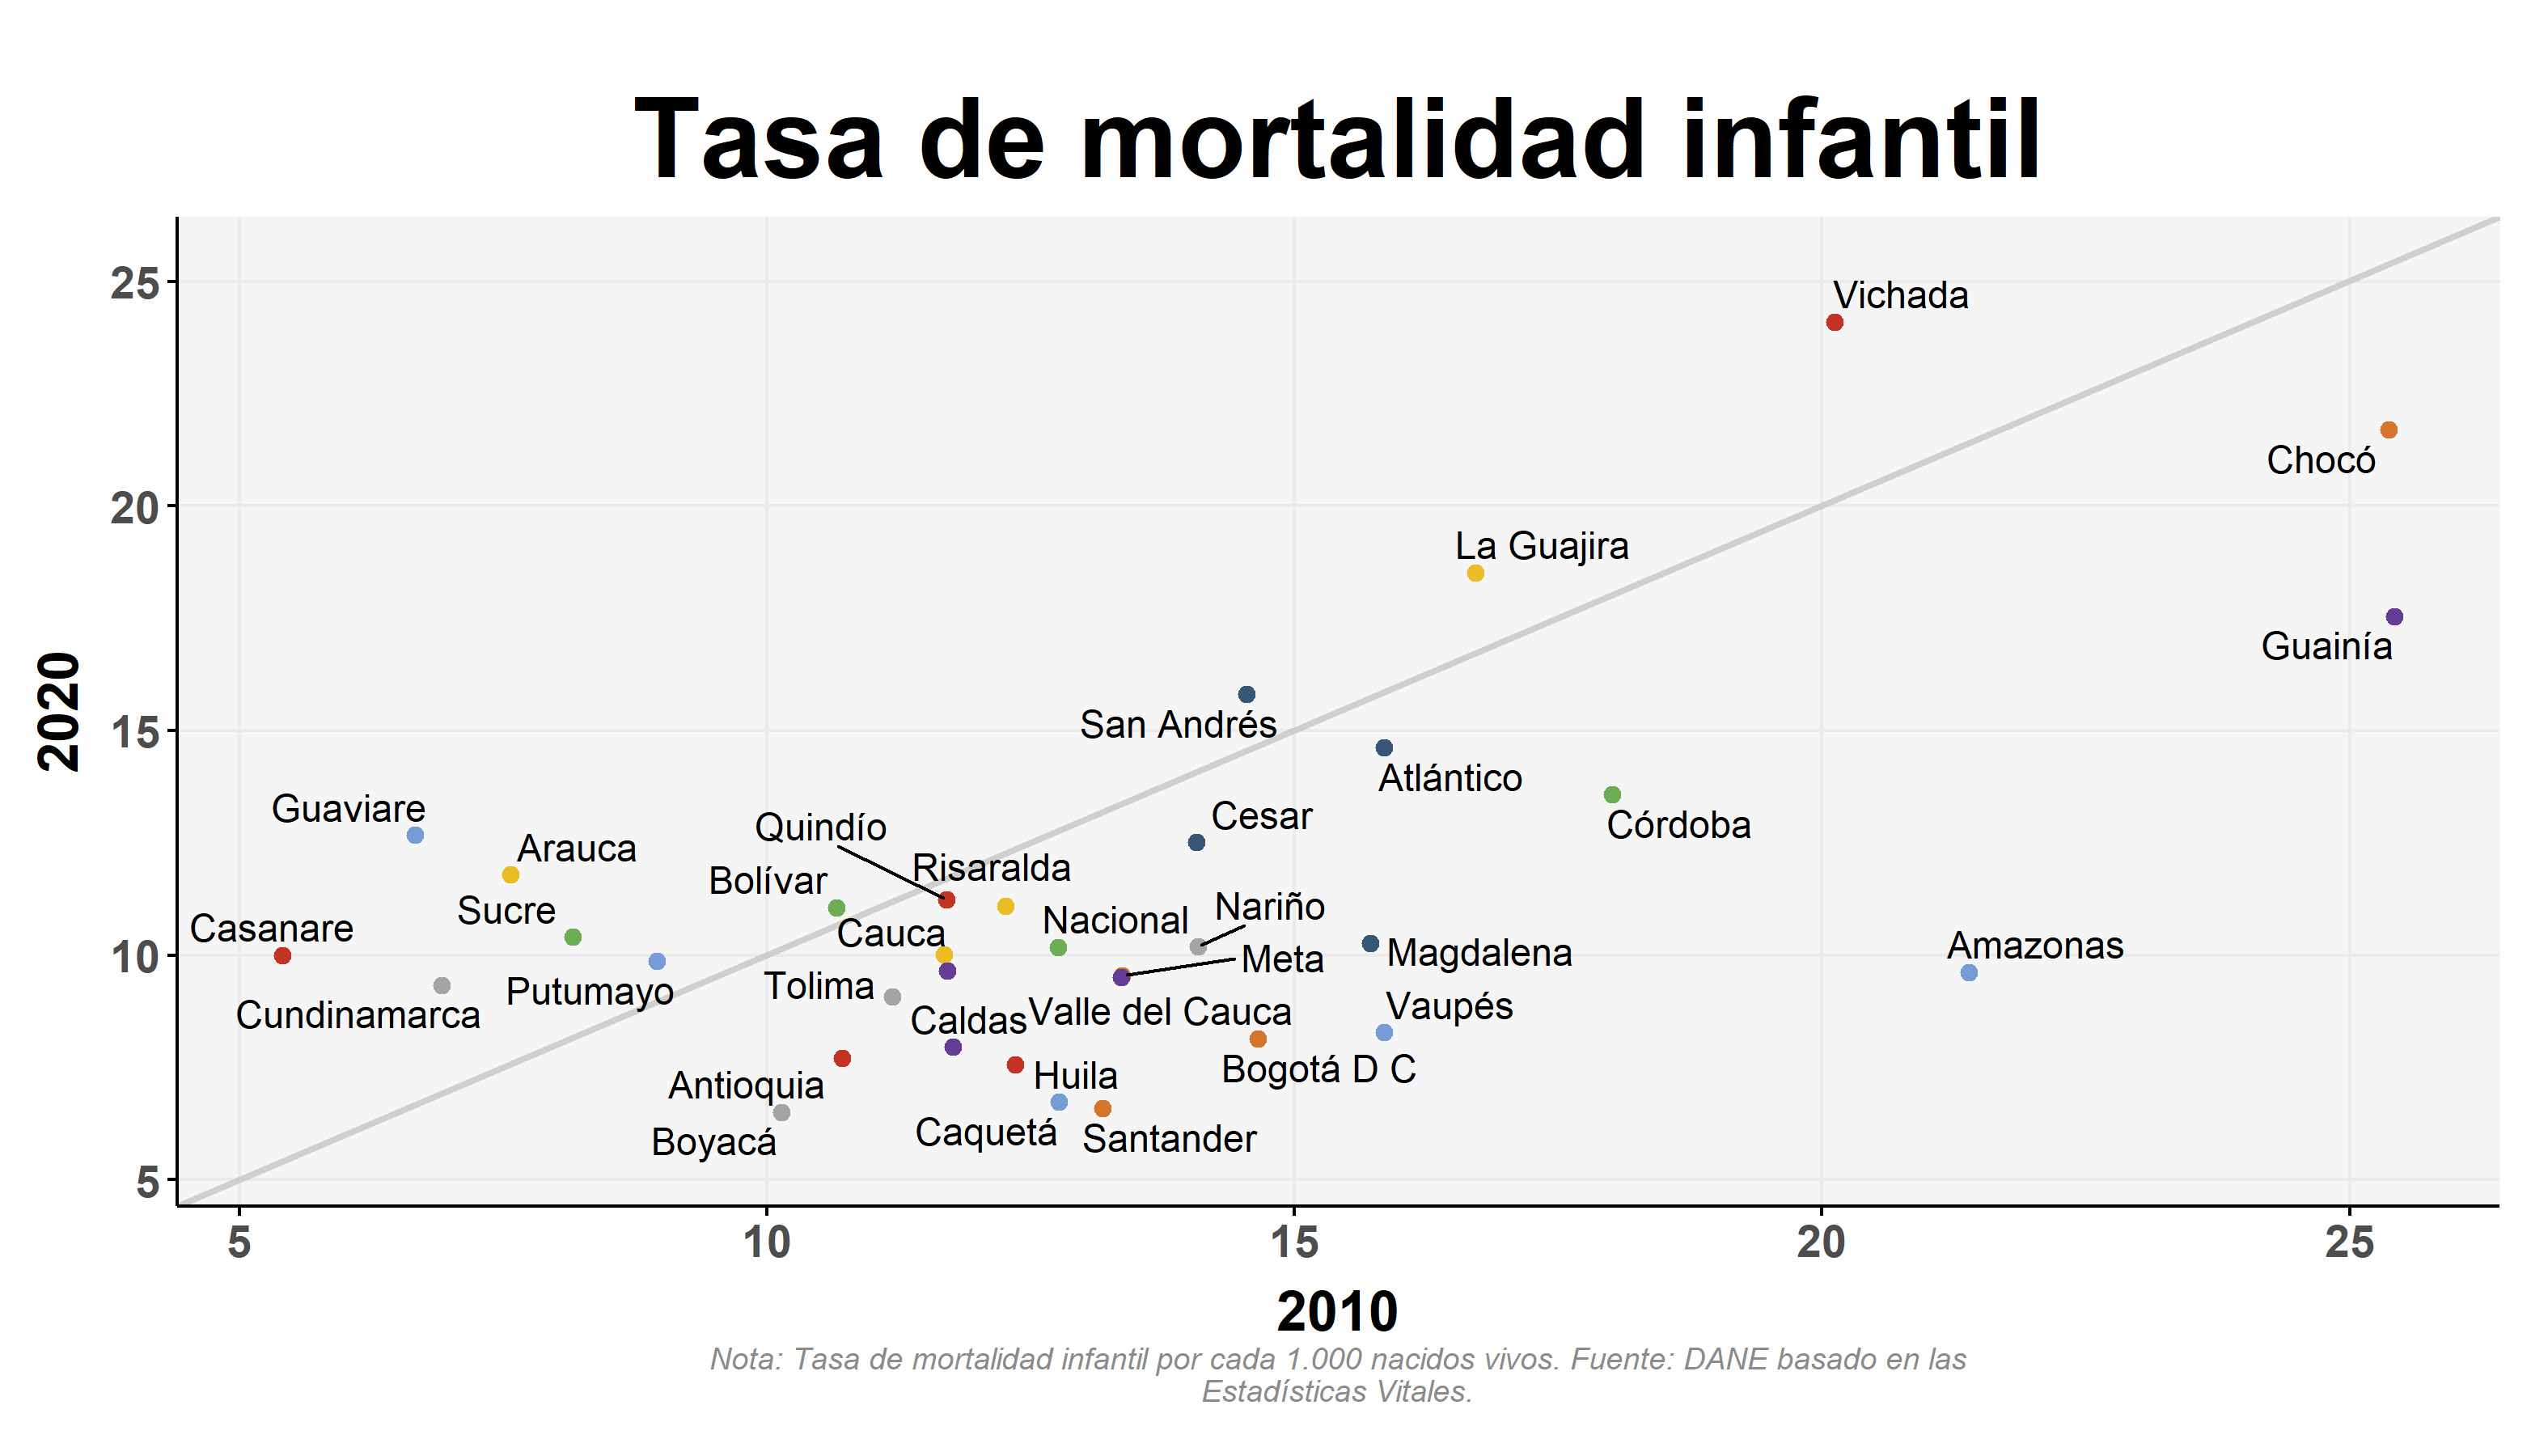
\includegraphics[width=\textwidth,keepaspectratio]{img/var_290_scatter_time.png}
        \end{center}
    \end{figure}
            \begin{itemize}
                    \item Gran parte de los dptos tienen una tasa de mortalidad menor a 15.
                    \item Vichada, Guaviare, Cundinamarca, Casanare, Arauca y La Guajira se encuentran en los dptos que aumentaron su tasa de mortalidad infantil para 2020 con respecto a la de 2010.
                    \item Vichada, Chocó, La Guajira y Guainía son los dptos con la tasa más alta para 2020, aunque Chocó y Guainía son los únicos que presentaron mejoras con respecto a 2010.
                    \item Amazonas es el que tuvo la mayor mejora, pasando de valores por encima de 20 a estar cerca de una tasa de 10 menores de un año fallecidos por cada mil nacidos vivos, pasando de ser el tercer dpto con la tasa más alta en 2010 a estar alrededor del nivel nacional.
                \end{itemize}

%%%% Include figures
    \begin{figure}[H]
        \caption{Tasa de mortalidad infantil por departamentos para 2020 \label{map_result_2} }
        \begin{center}
        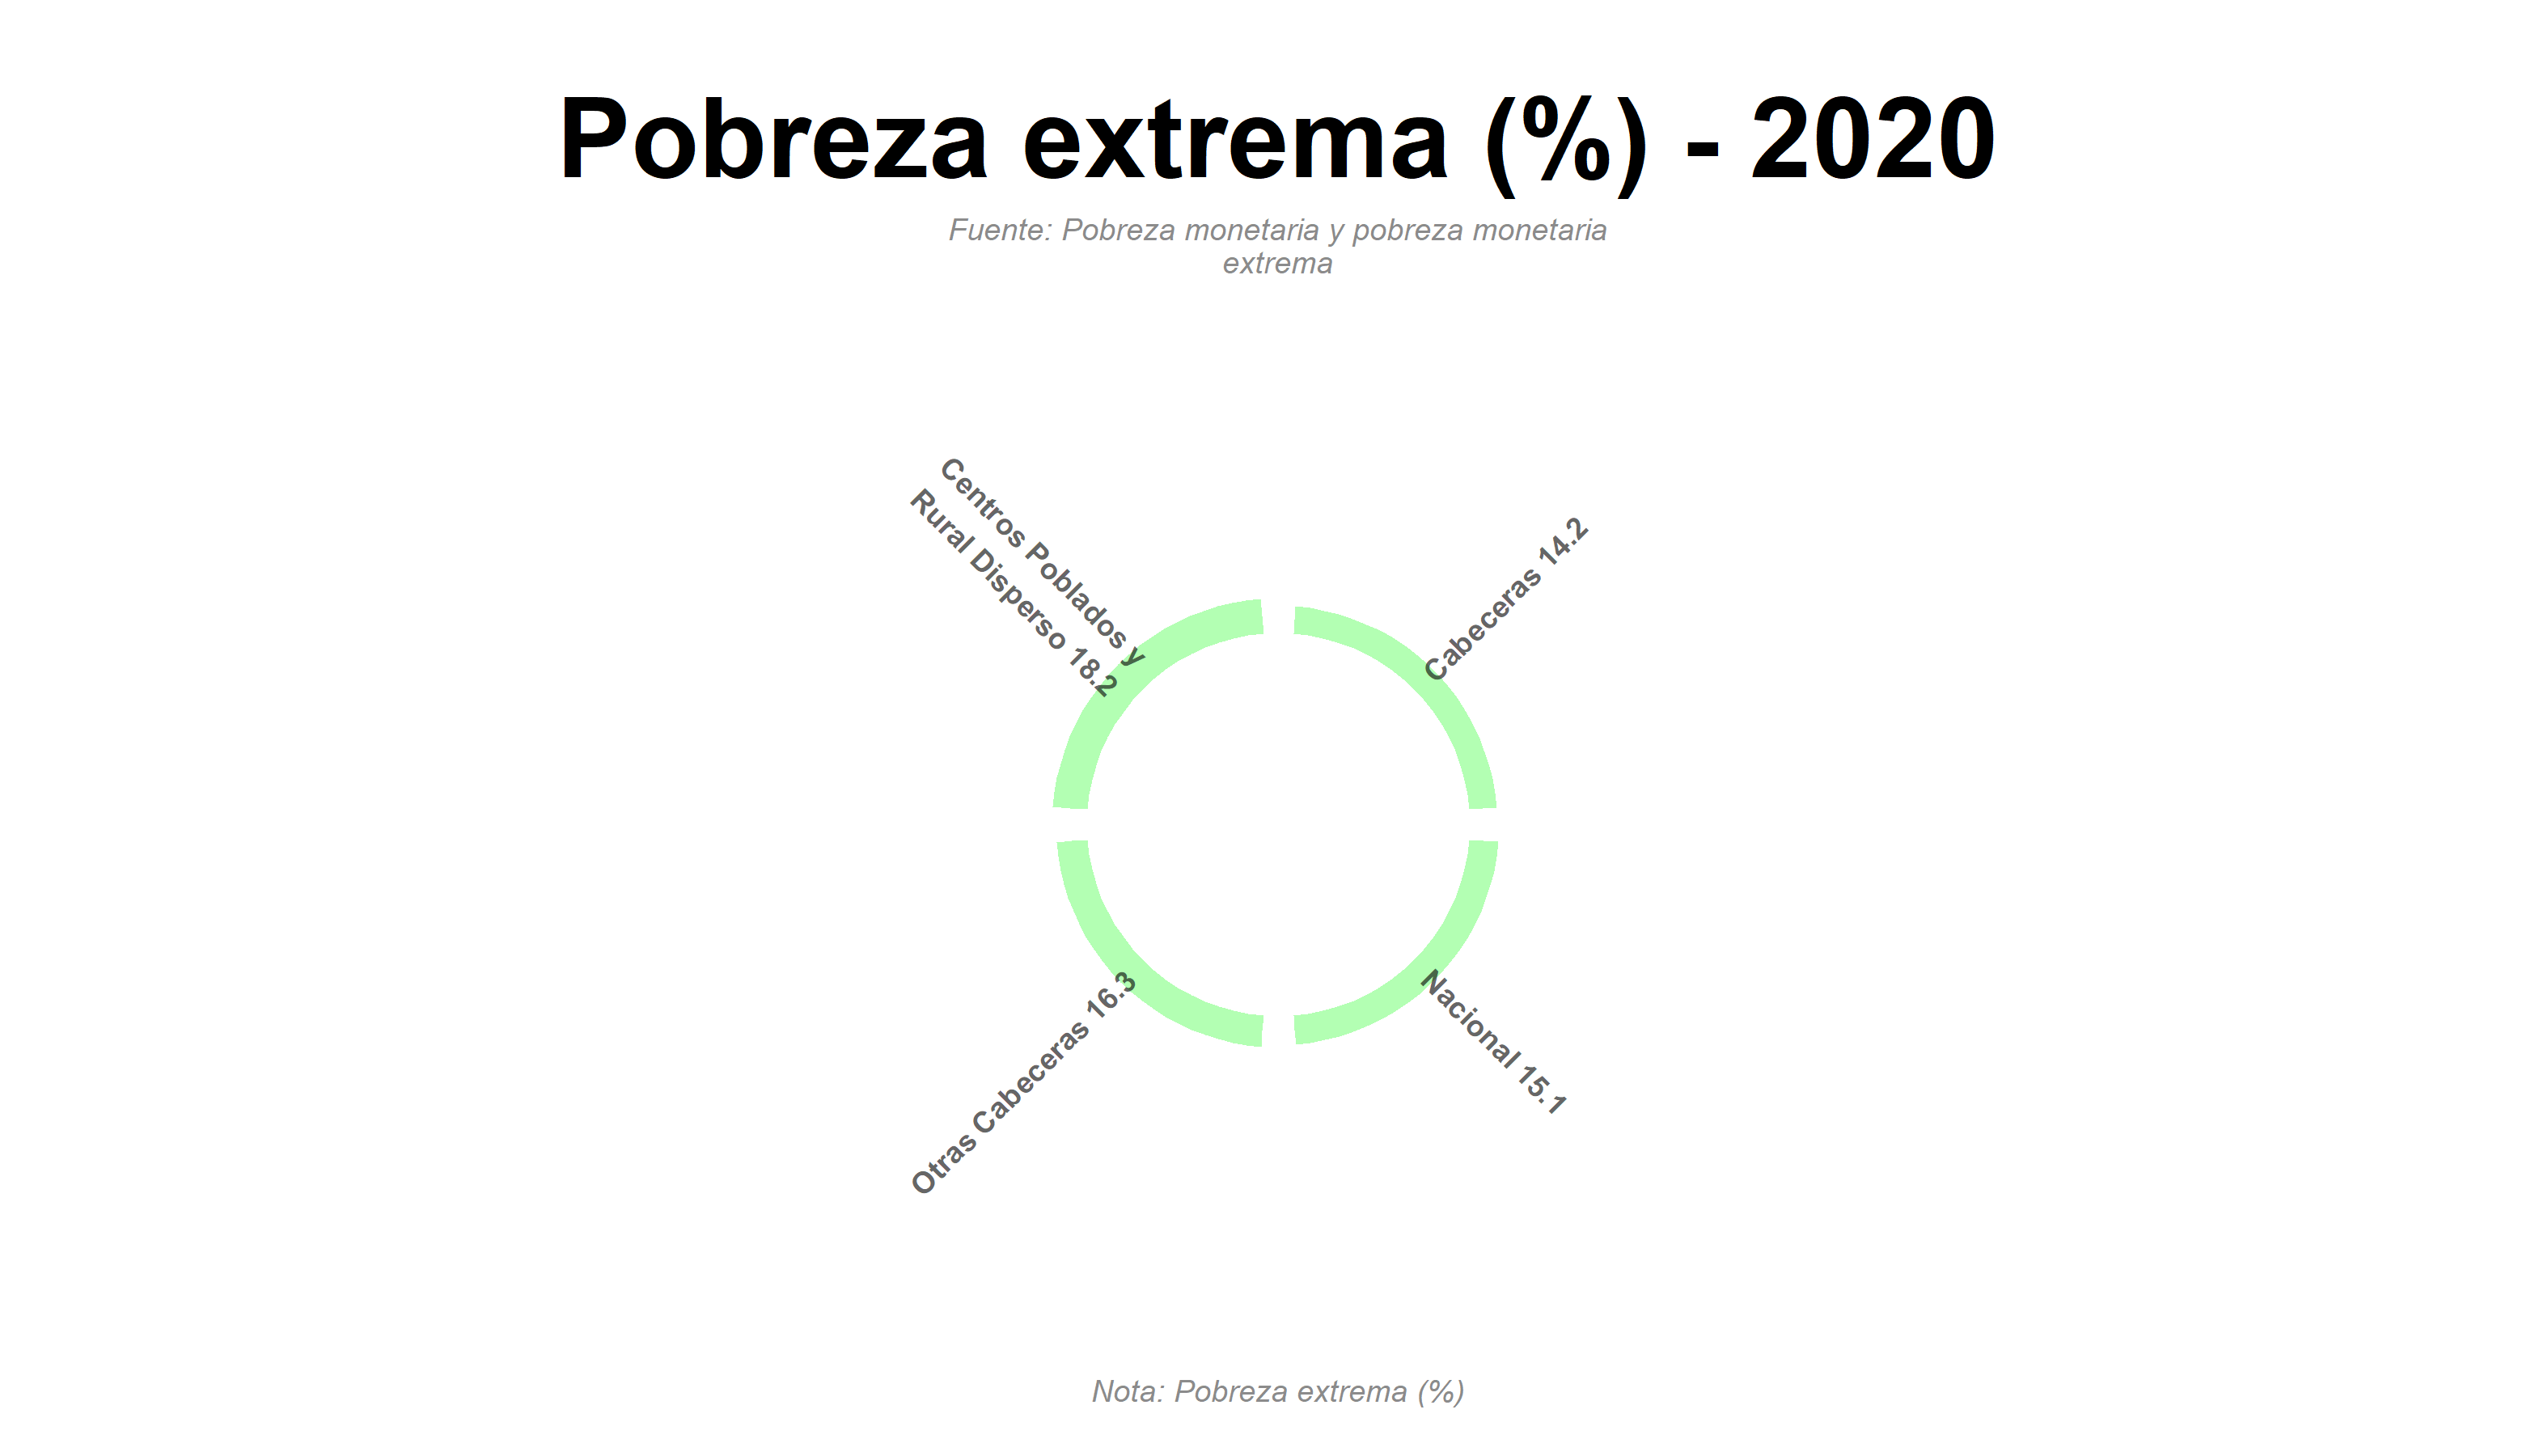
\includegraphics[width=\textwidth,keepaspectratio]{img/var_290_static.png}
        \end{center}
    \end{figure}
            \begin{itemize}
                    \item Los países con menor tasa de mortalidad infantil se concentran en el centro del país, mientras que los de mayor son aquellos históricamente vulnerables en la periferia.
                    \item En Boyacá fallecen 6.5 niños menores de 1 año por cada mil nacidos vivos, siendo el dpto con menor tasa, por otro lado Vichada es el de mayor, siendo casi 4 veces Boyacá (24.1\%).
                    \end{itemize}

%%%% Include figures
    \begin{figure}[H]
        \caption{Tasa de mortalidad infantil a nivel nacional \label{map_result_2} }
        \begin{center}
        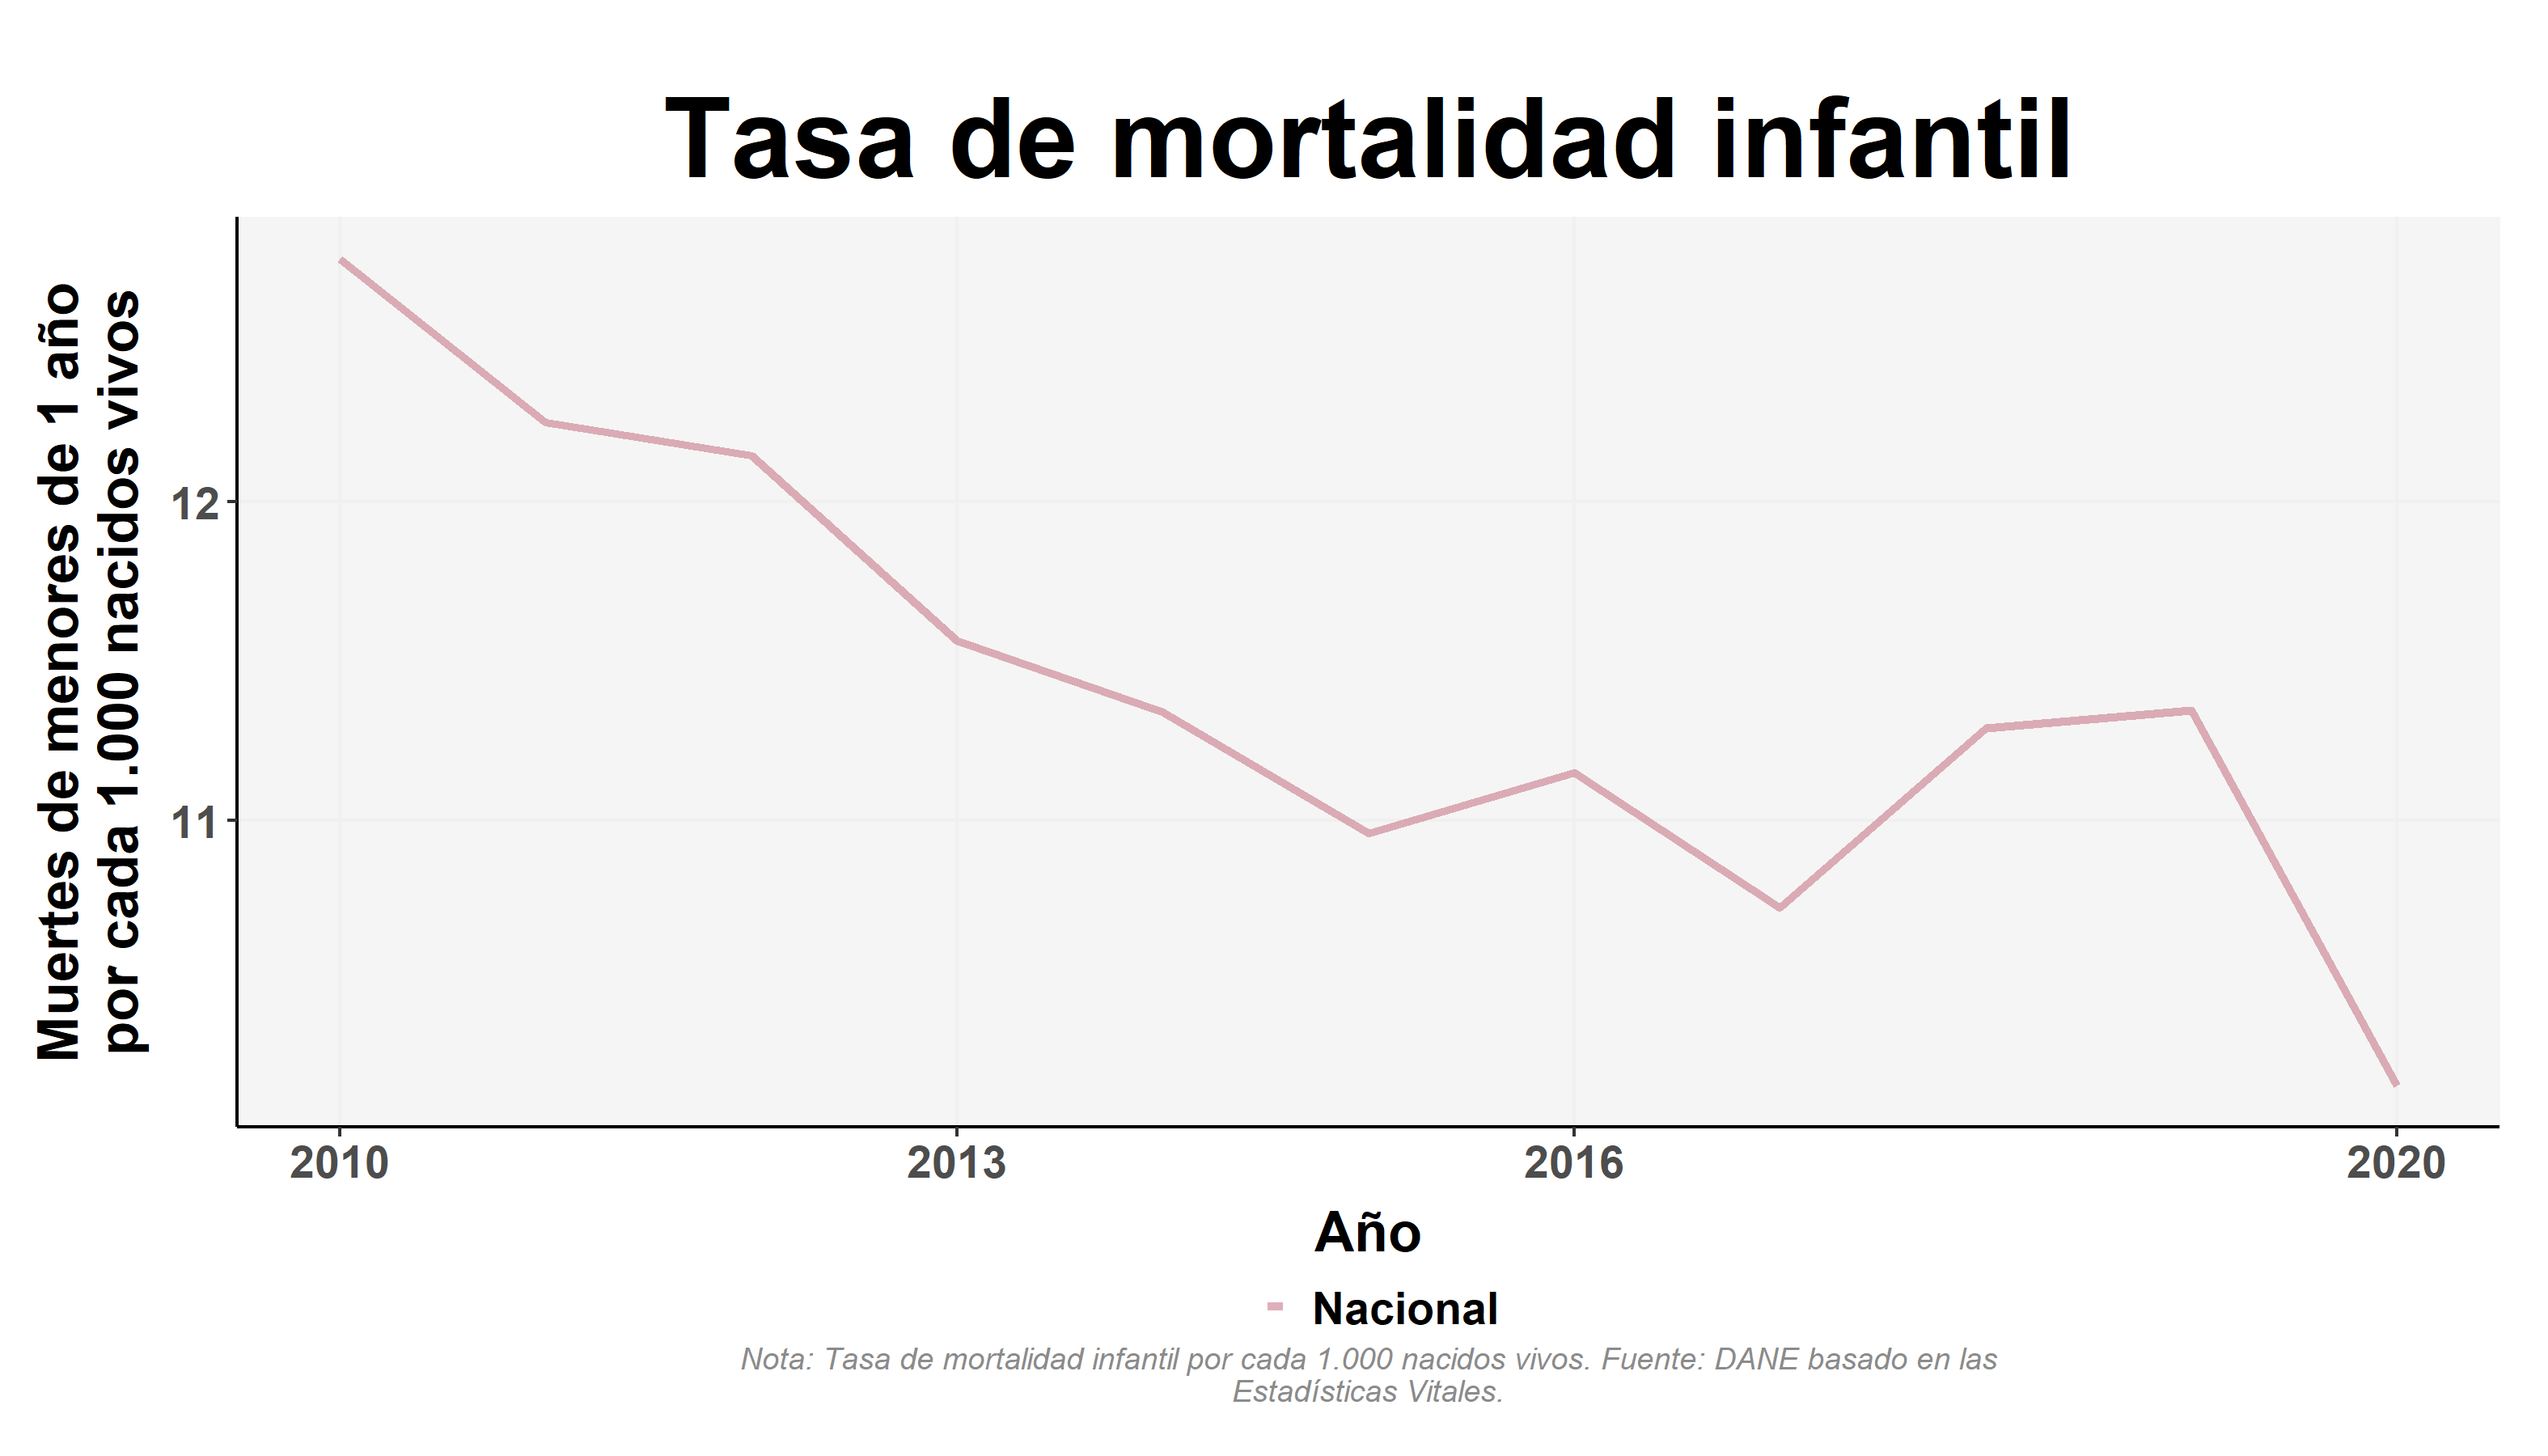
\includegraphics[width=\textwidth,keepaspectratio]{img/var_291_trend.png}
        \end{center}
    \end{figure}
            \begin{itemize}
                    \item La tasa a nivel nacional ha ido disminuyendo en los últimos 10 años.
                    \item Vemos dos picos leves en 2016 y 2018-2019, pero para 2020 se evidencia una caída abrupta compensando el retroceso del 2018-2019.
                \end{itemize}

    \subsection{Asistencia escolar, preescolar y primaria}
        \subsubsection{PENDIENTE - Asistencia escolar de menores de 5 años}

%%%% Include figures
    \begin{figure}[H]
        \caption{Asistencia escolar de menores de 5 años por departamentos - 2010 VS 2020 \label{map_result_2} }
        \begin{center}
        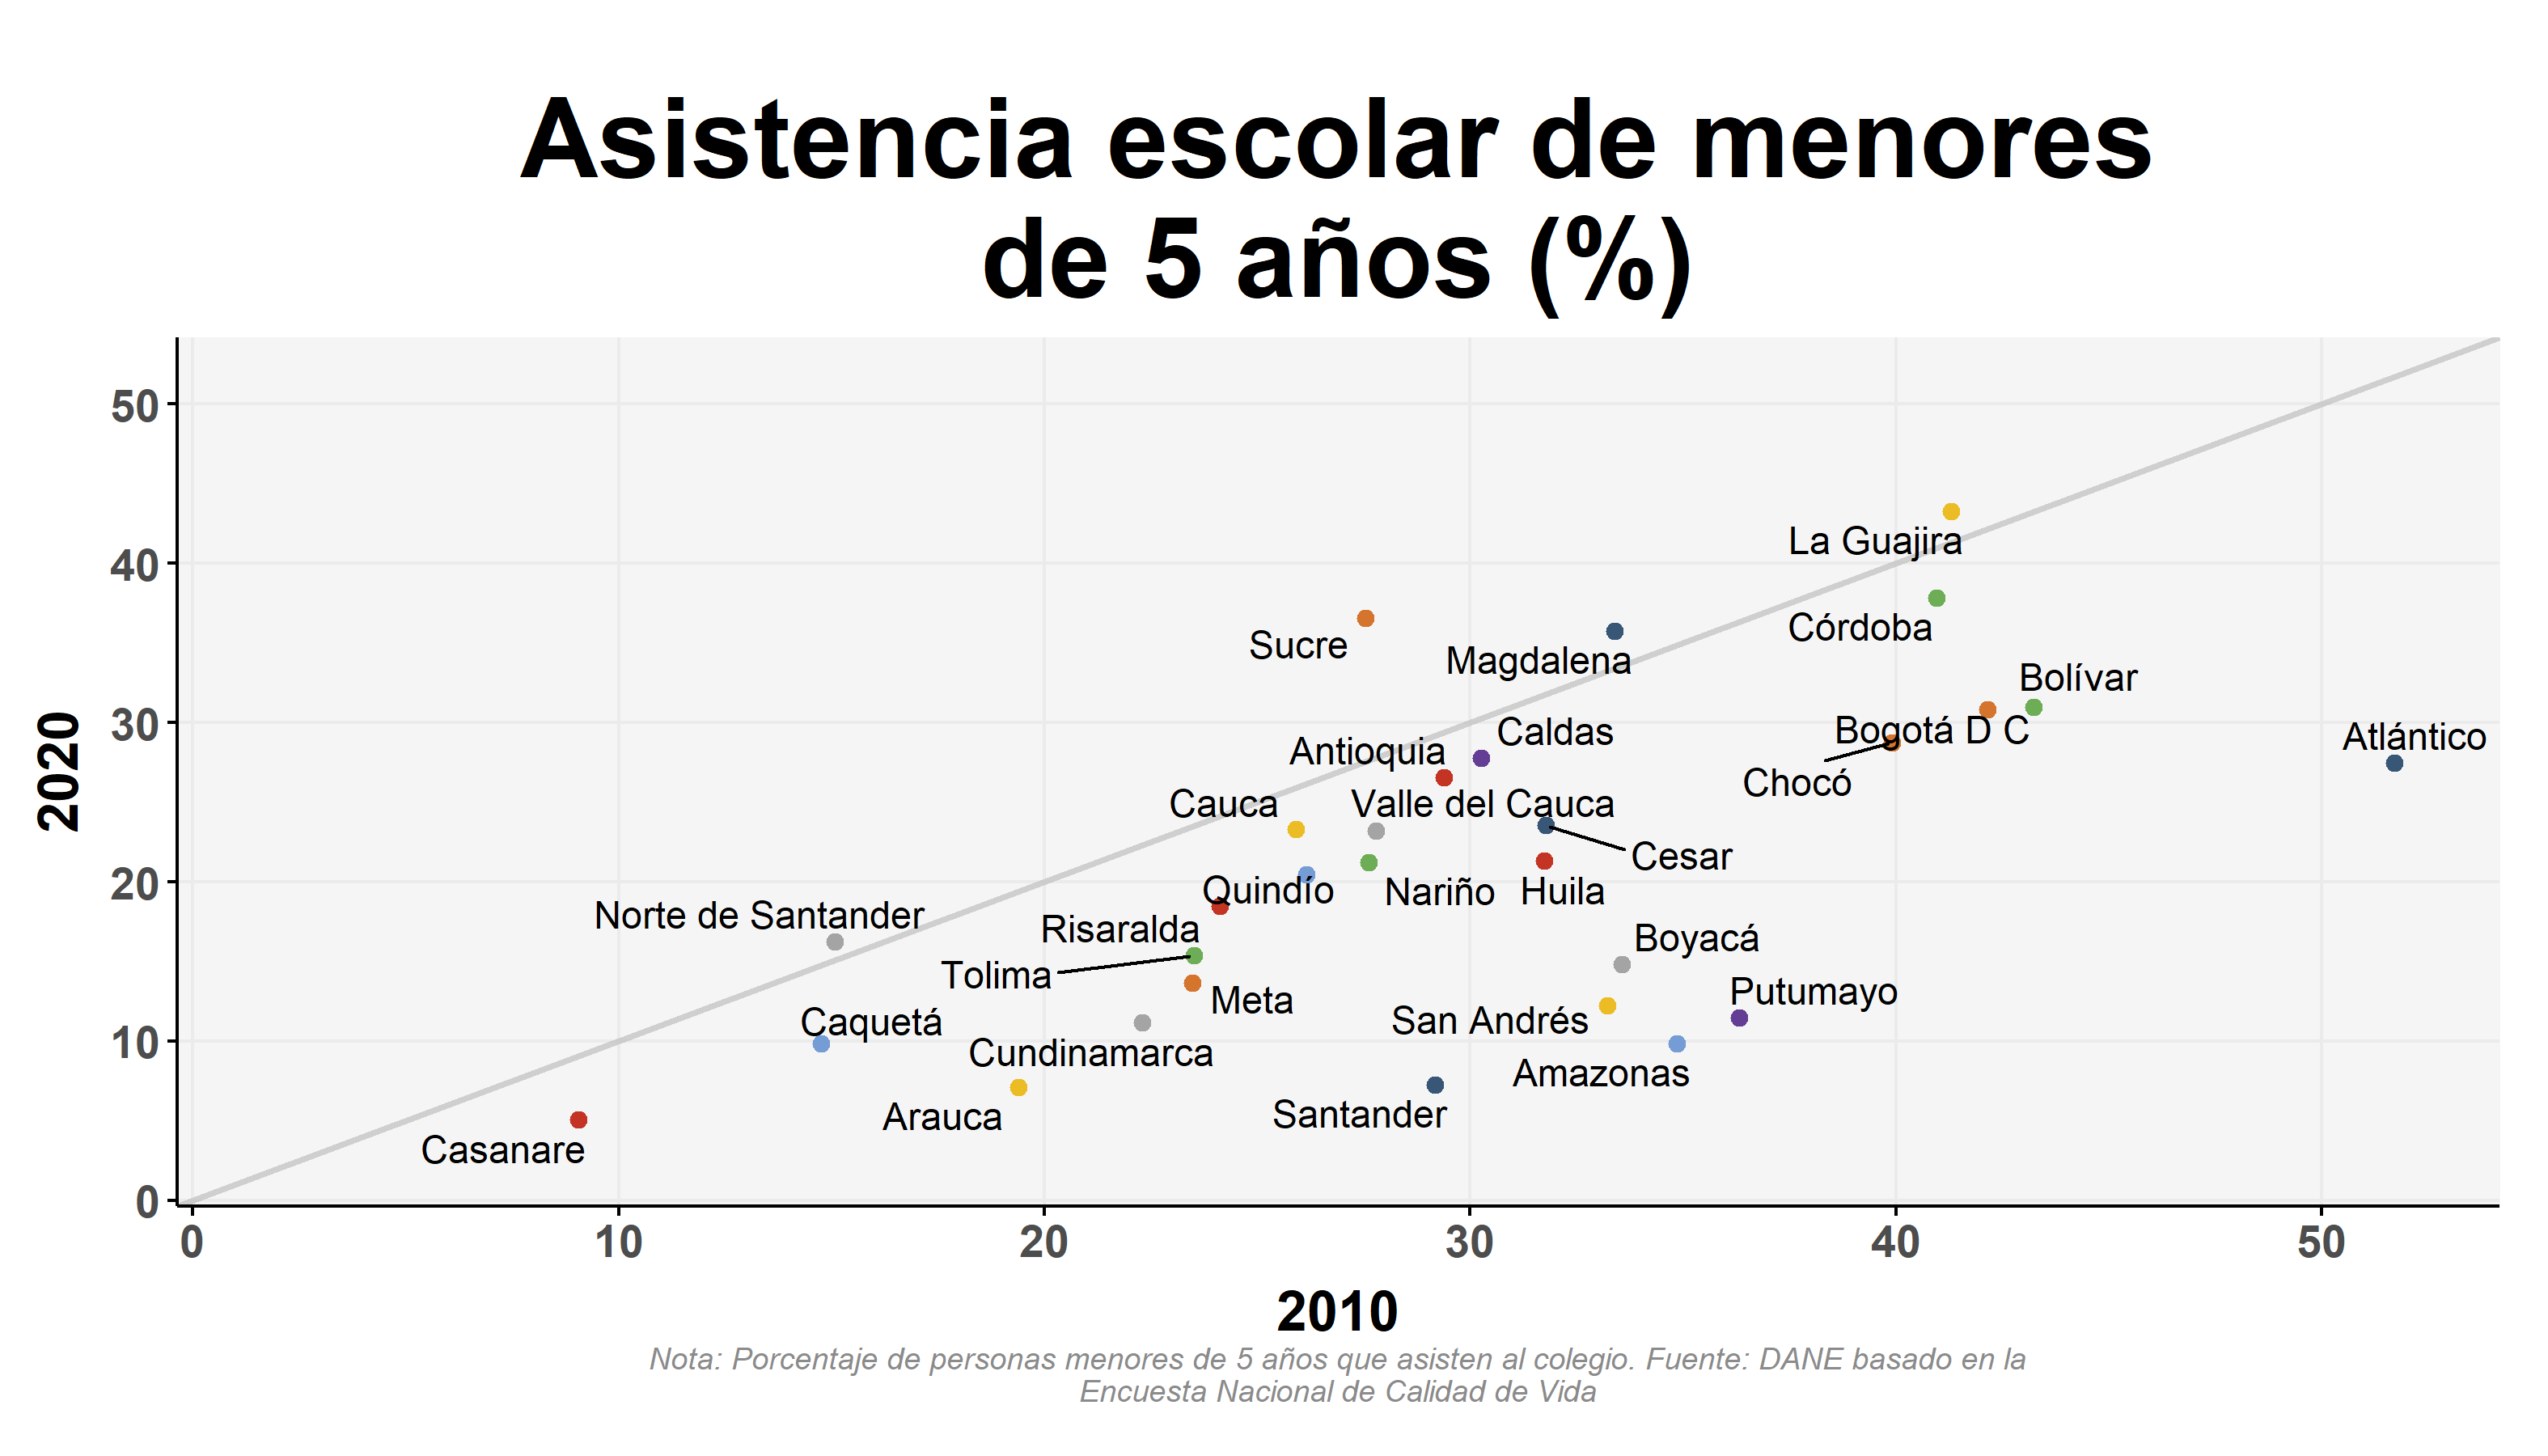
\includegraphics[width=\textwidth,keepaspectratio]{img/var_99_scatter_time.png}
        \end{center}
    \end{figure}
            \begin{itemize}
                \item Solo Sucre, Magdalena, La Guajira y Norte tienen niveles superiores para 2020 comparados con los del 2010, el resto de dptos desmejoraron en estos diez años.
                \item Atlántico, Santander, Boyacá, Putumayo y Amazonas son los dptos que tuvieron la mayor desmejora (disminución del más del 52\% según la gráfica map change 99)
                \item Atlántico pasó de ser el de mayor cobertura en 2010, teniendo una diferencia cercana a 10\% con el segundo mejor, con más del 50\% a estar por debajo de 30\%.
                \end{itemize}

%%%% Include figures
    \begin{figure}[H]
        \caption{Asistencia escolar de menores de 5 años por departamentos para 2020 \label{map_result_2} }
        \begin{center}
        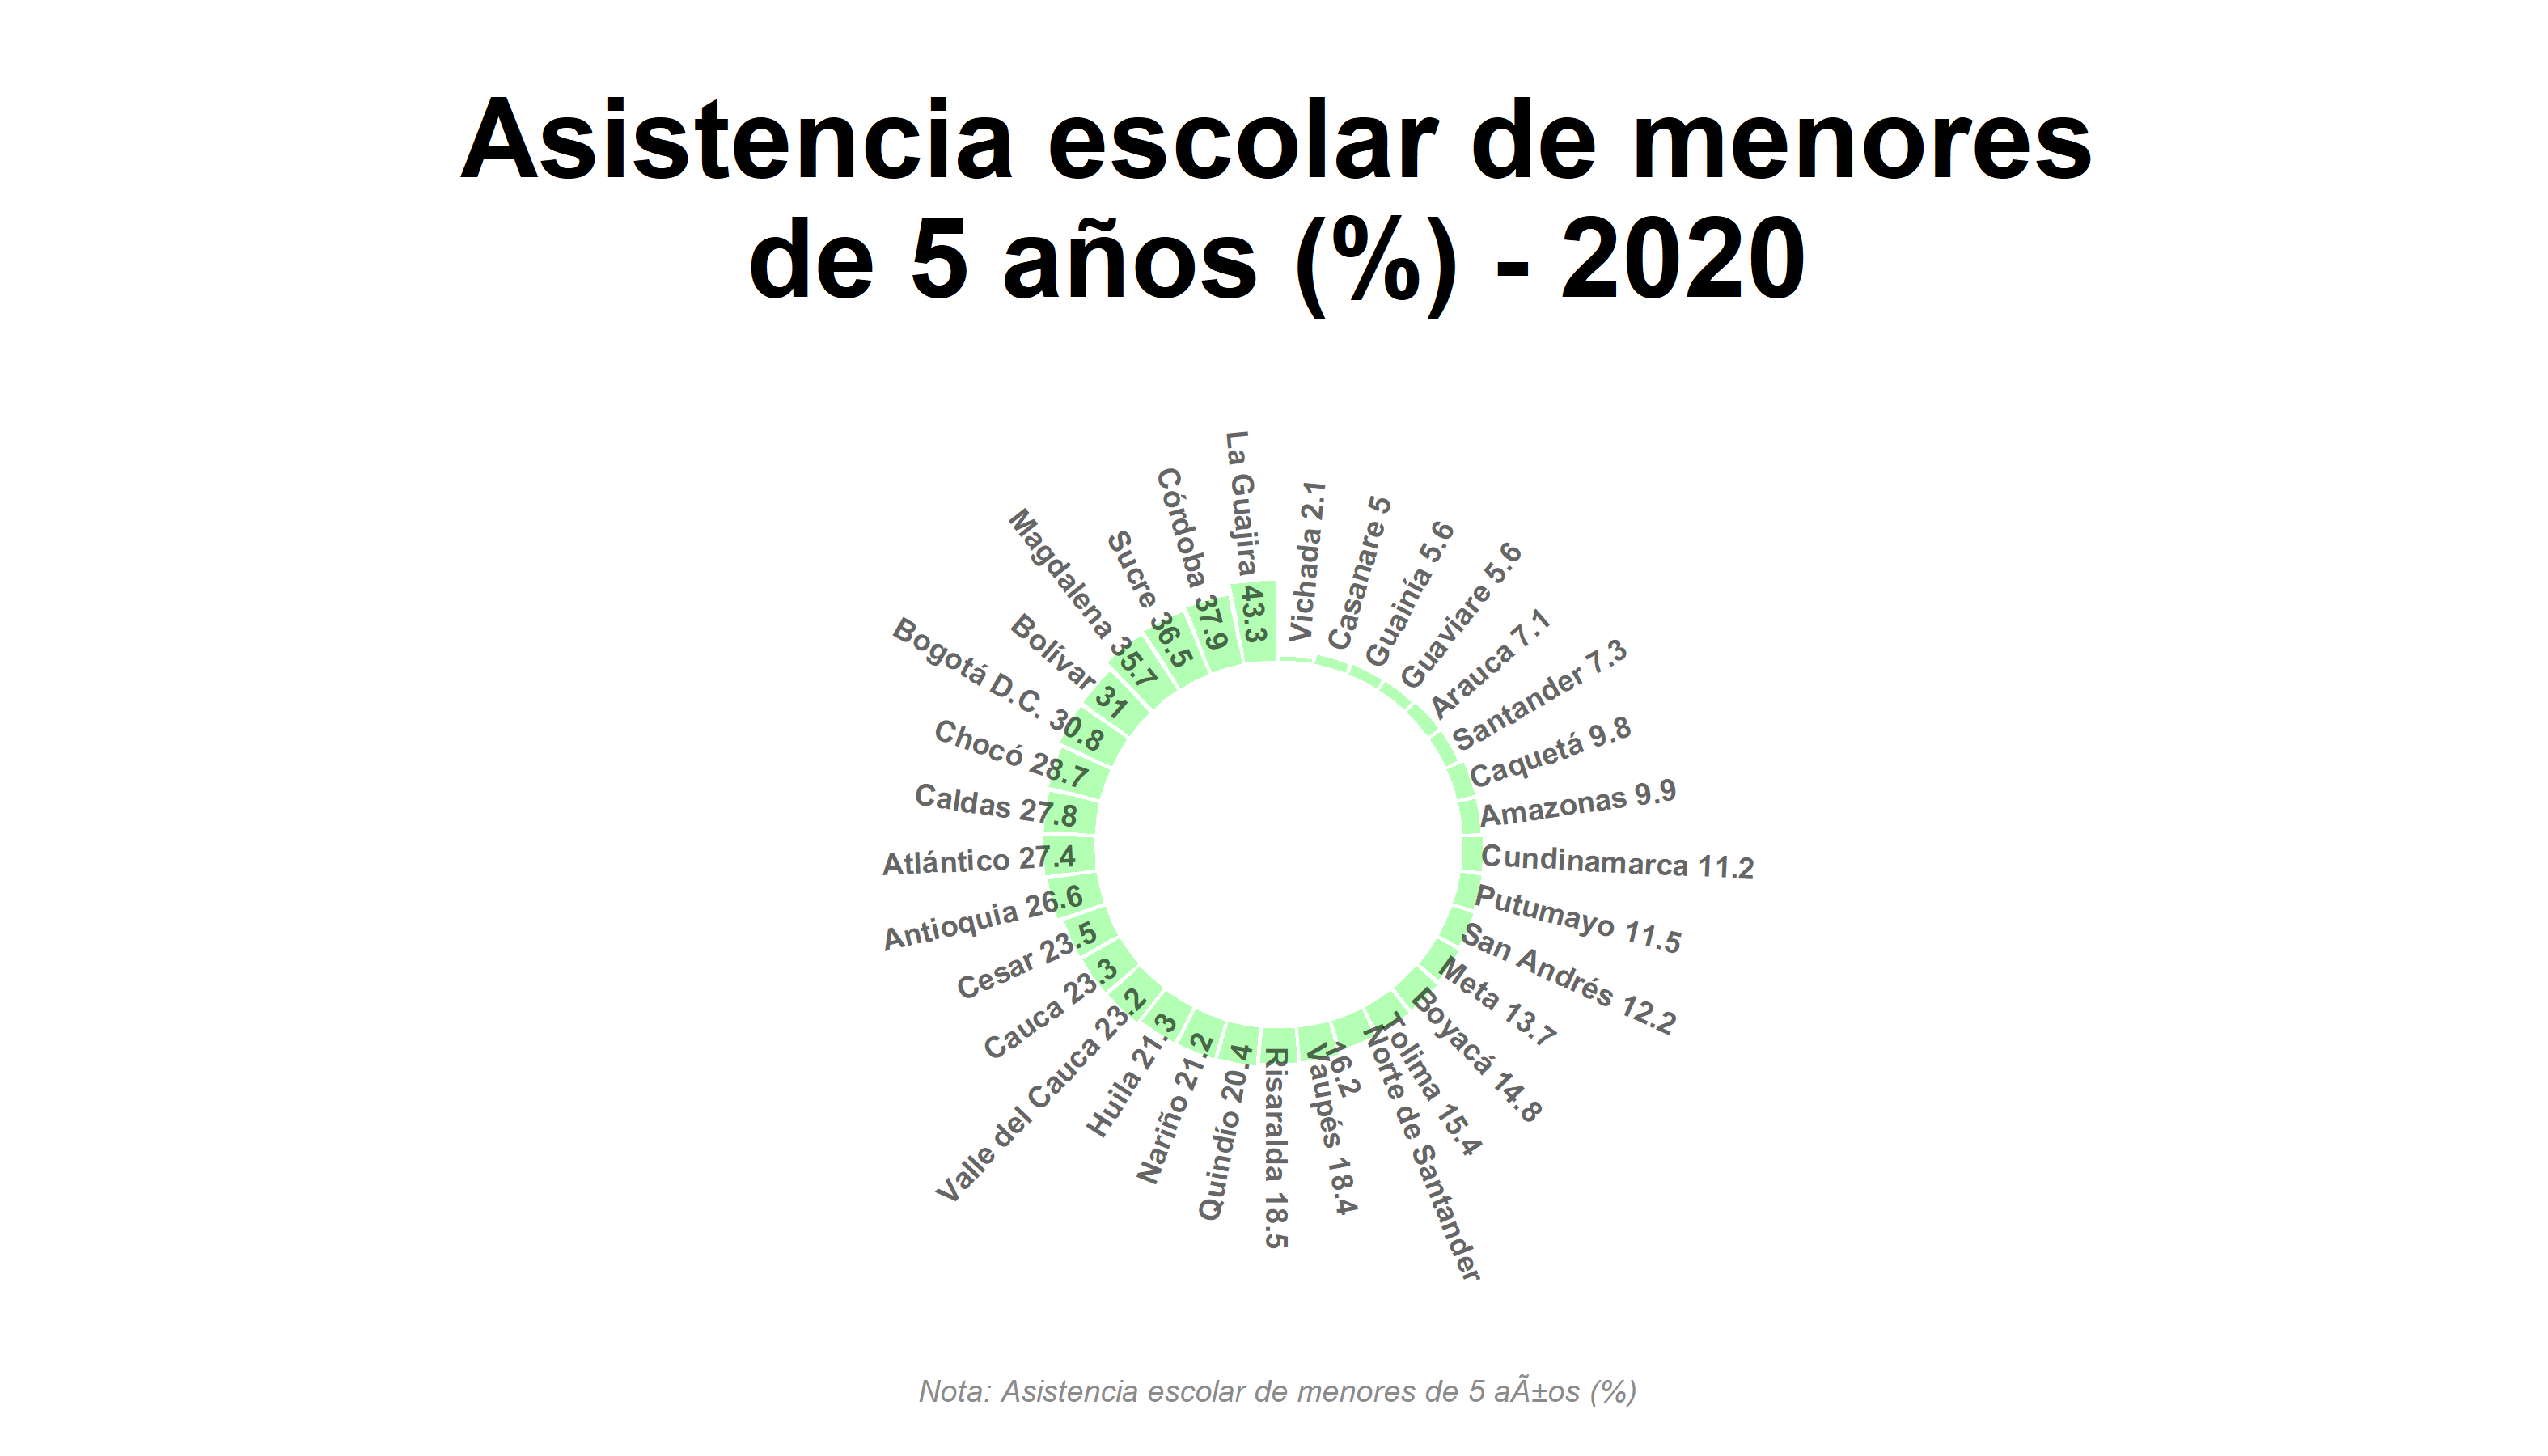
\includegraphics[width=\textwidth,keepaspectratio]{img/var_99_static.png}
        \end{center}
    \end{figure}
            \begin{itemize}
                \item Hay una gran heterogeneidad entre los territorios, yendo desde un menos de un 3\% hasta cerca del 50\%.
                \item Mientras que en Vichada solo el 2.1\% de los menores de 5 año asisten a algún centro educativo, en La Guajira son el 43.3\%, teniendo una diferencia de cerca del 40\%.
                \item La concentración de los territorios con menor cobertura en 2020 se encuentran en la zona amazónica y oriental del país (gráfica map 99).
                \end{itemize}

%%%% Include figures
    \begin{figure}[H]
        \caption{Asistencia escolar de menores de 5 años por zonas \label{map_result_2} }
        \begin{center}
        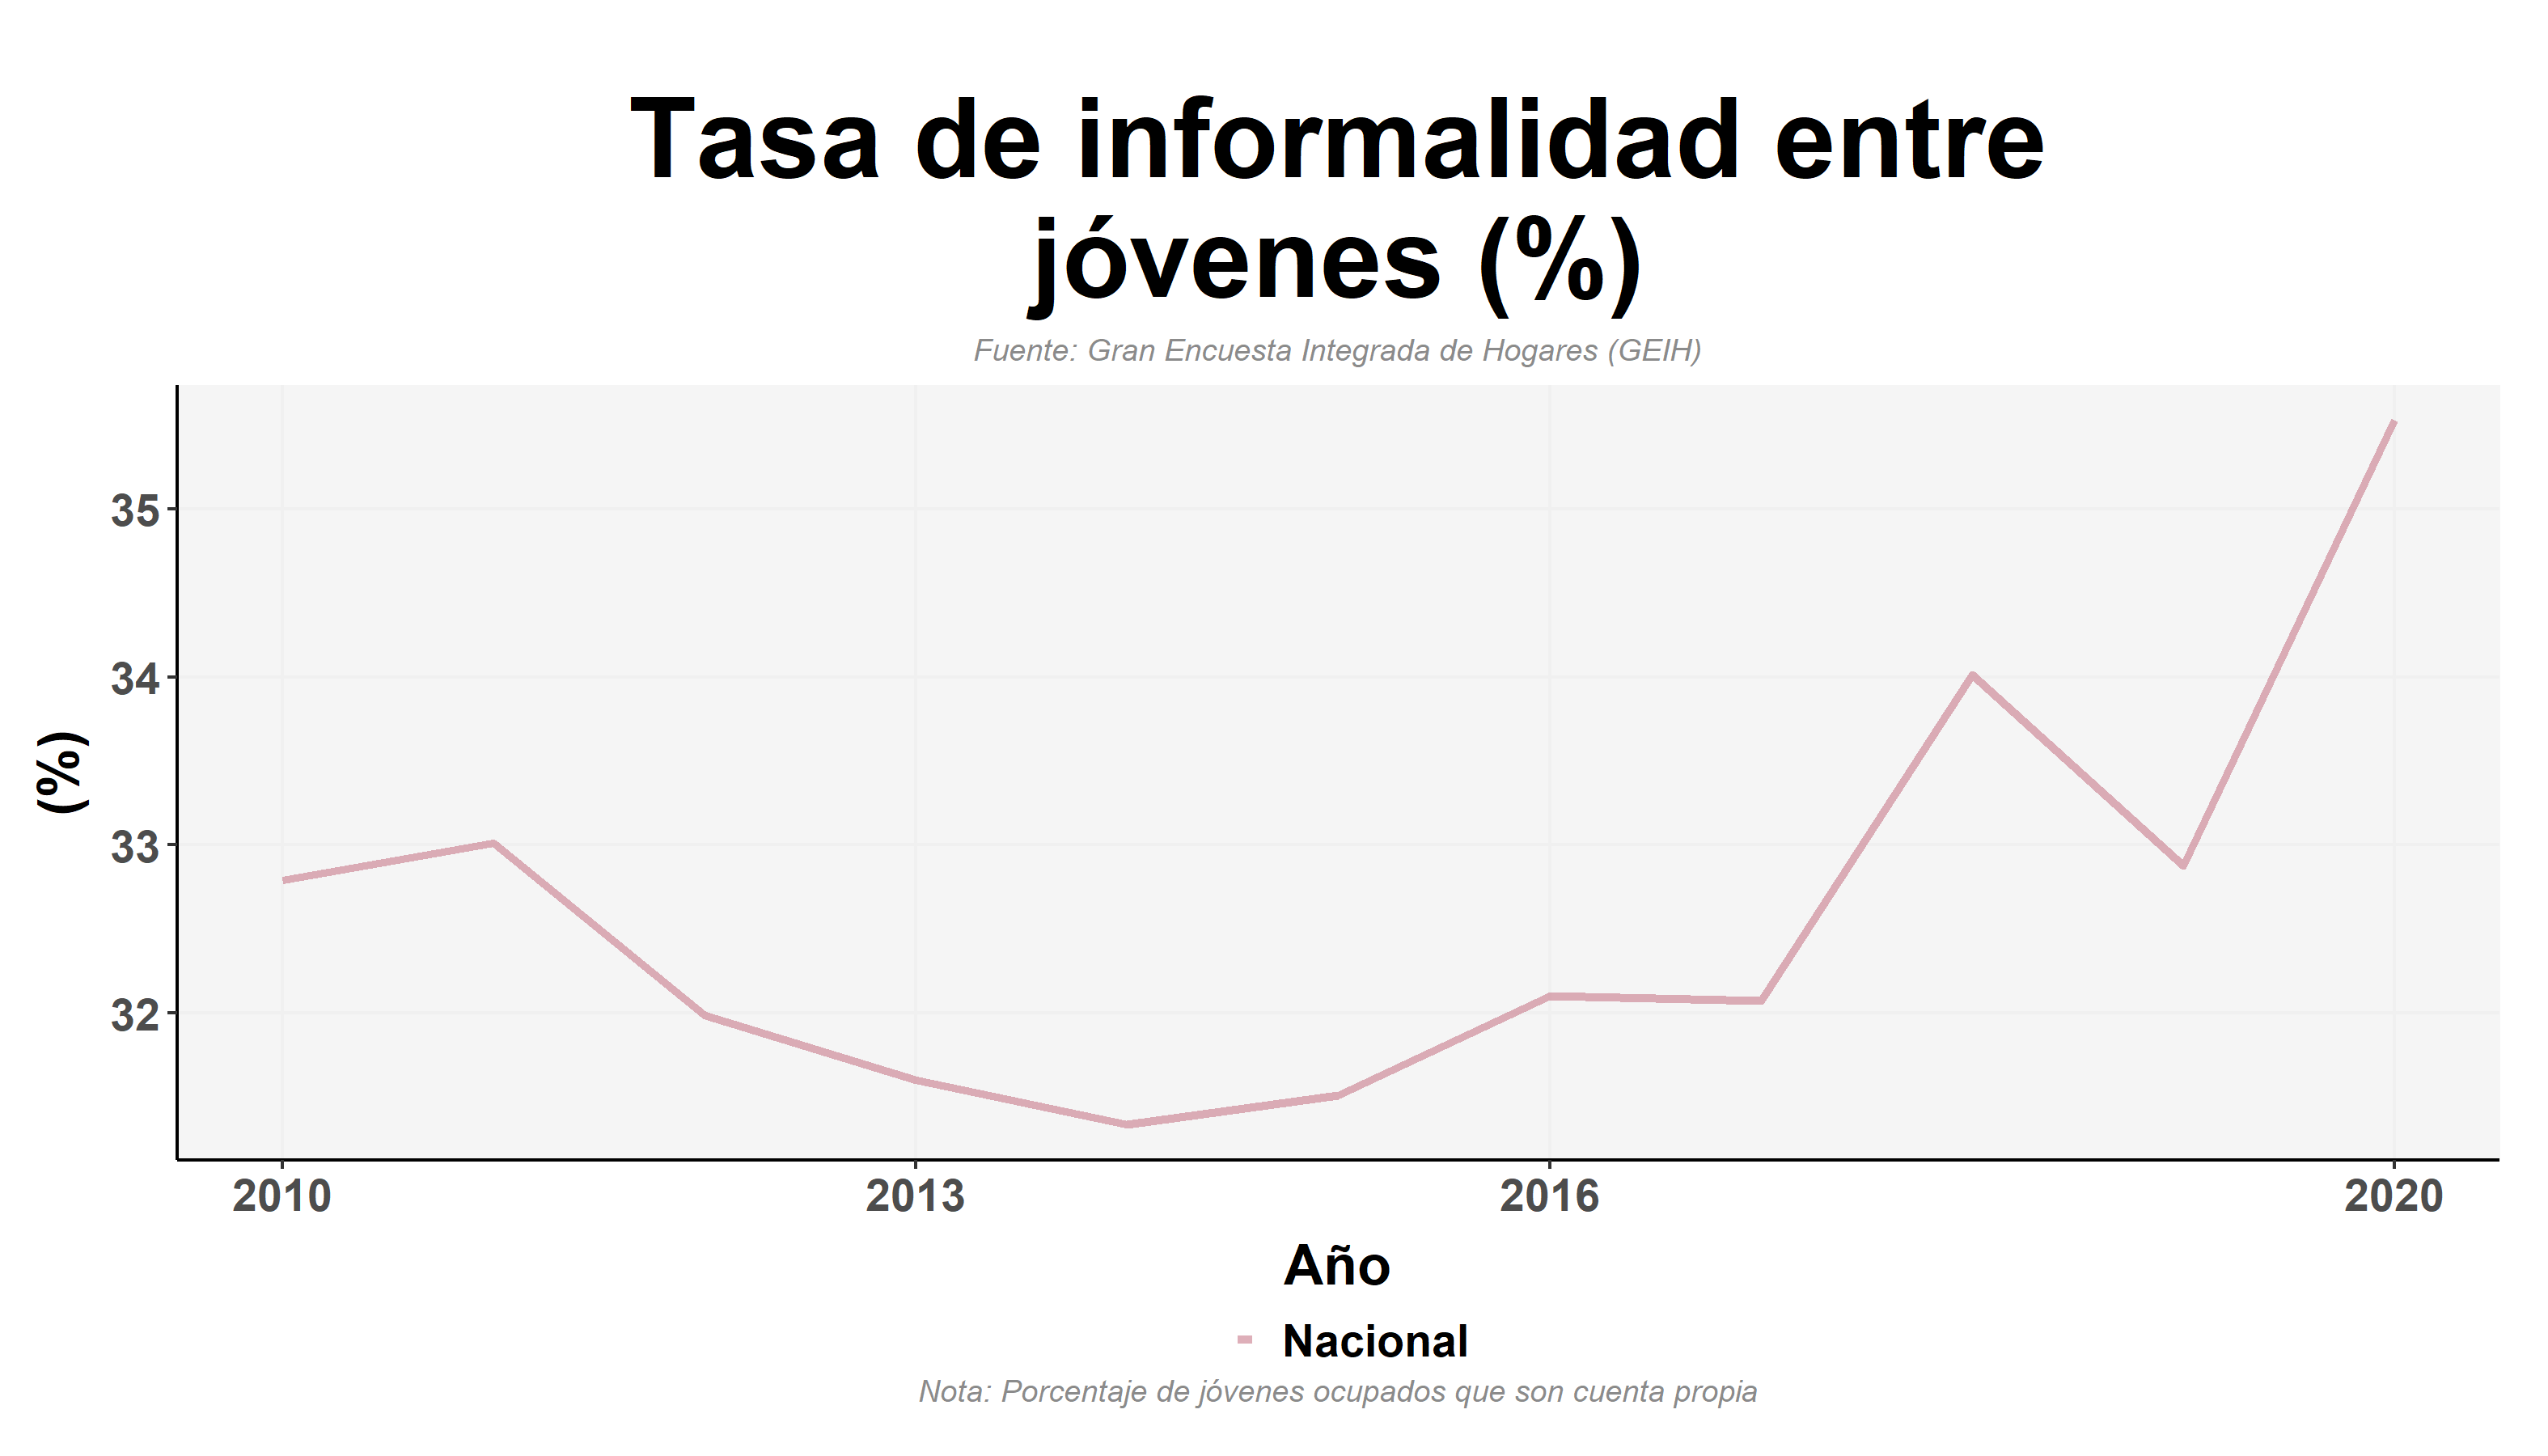
\includegraphics[width=\textwidth,keepaspectratio]{img/var_100_trend.png}
        \end{center}
    \end{figure}
            \begin{itemize}
                \item La asistencia escolar de menores de 5 años en zonas urbanas es casi el doble que en las rurales.
                \item La brecha se había mantenido en el tiempo hasta el 2020, donde disminuyó significativamente.
                \item En 2020 se observó una caída en la asistencia en la zonas urbanas, llevando a presentar valores cercanos a los rurales en el año anterior. La zona rural también presentó una disminución pero no tan abrupta.
                \item Ambas zonas presentan porcentajes de asistencia menores para 2020 que los presentados en 2010, siendo aún más la diferencia en la zona urbana.
                \end{itemize}

%%%% Include figures
    \begin{figure}[H]
        \caption{Asistencia escolar de menores de 5 años para el primer quintil de ingreso por departamentos - 2010 VS 2020 \label{map_result_2} }
        \begin{center}
        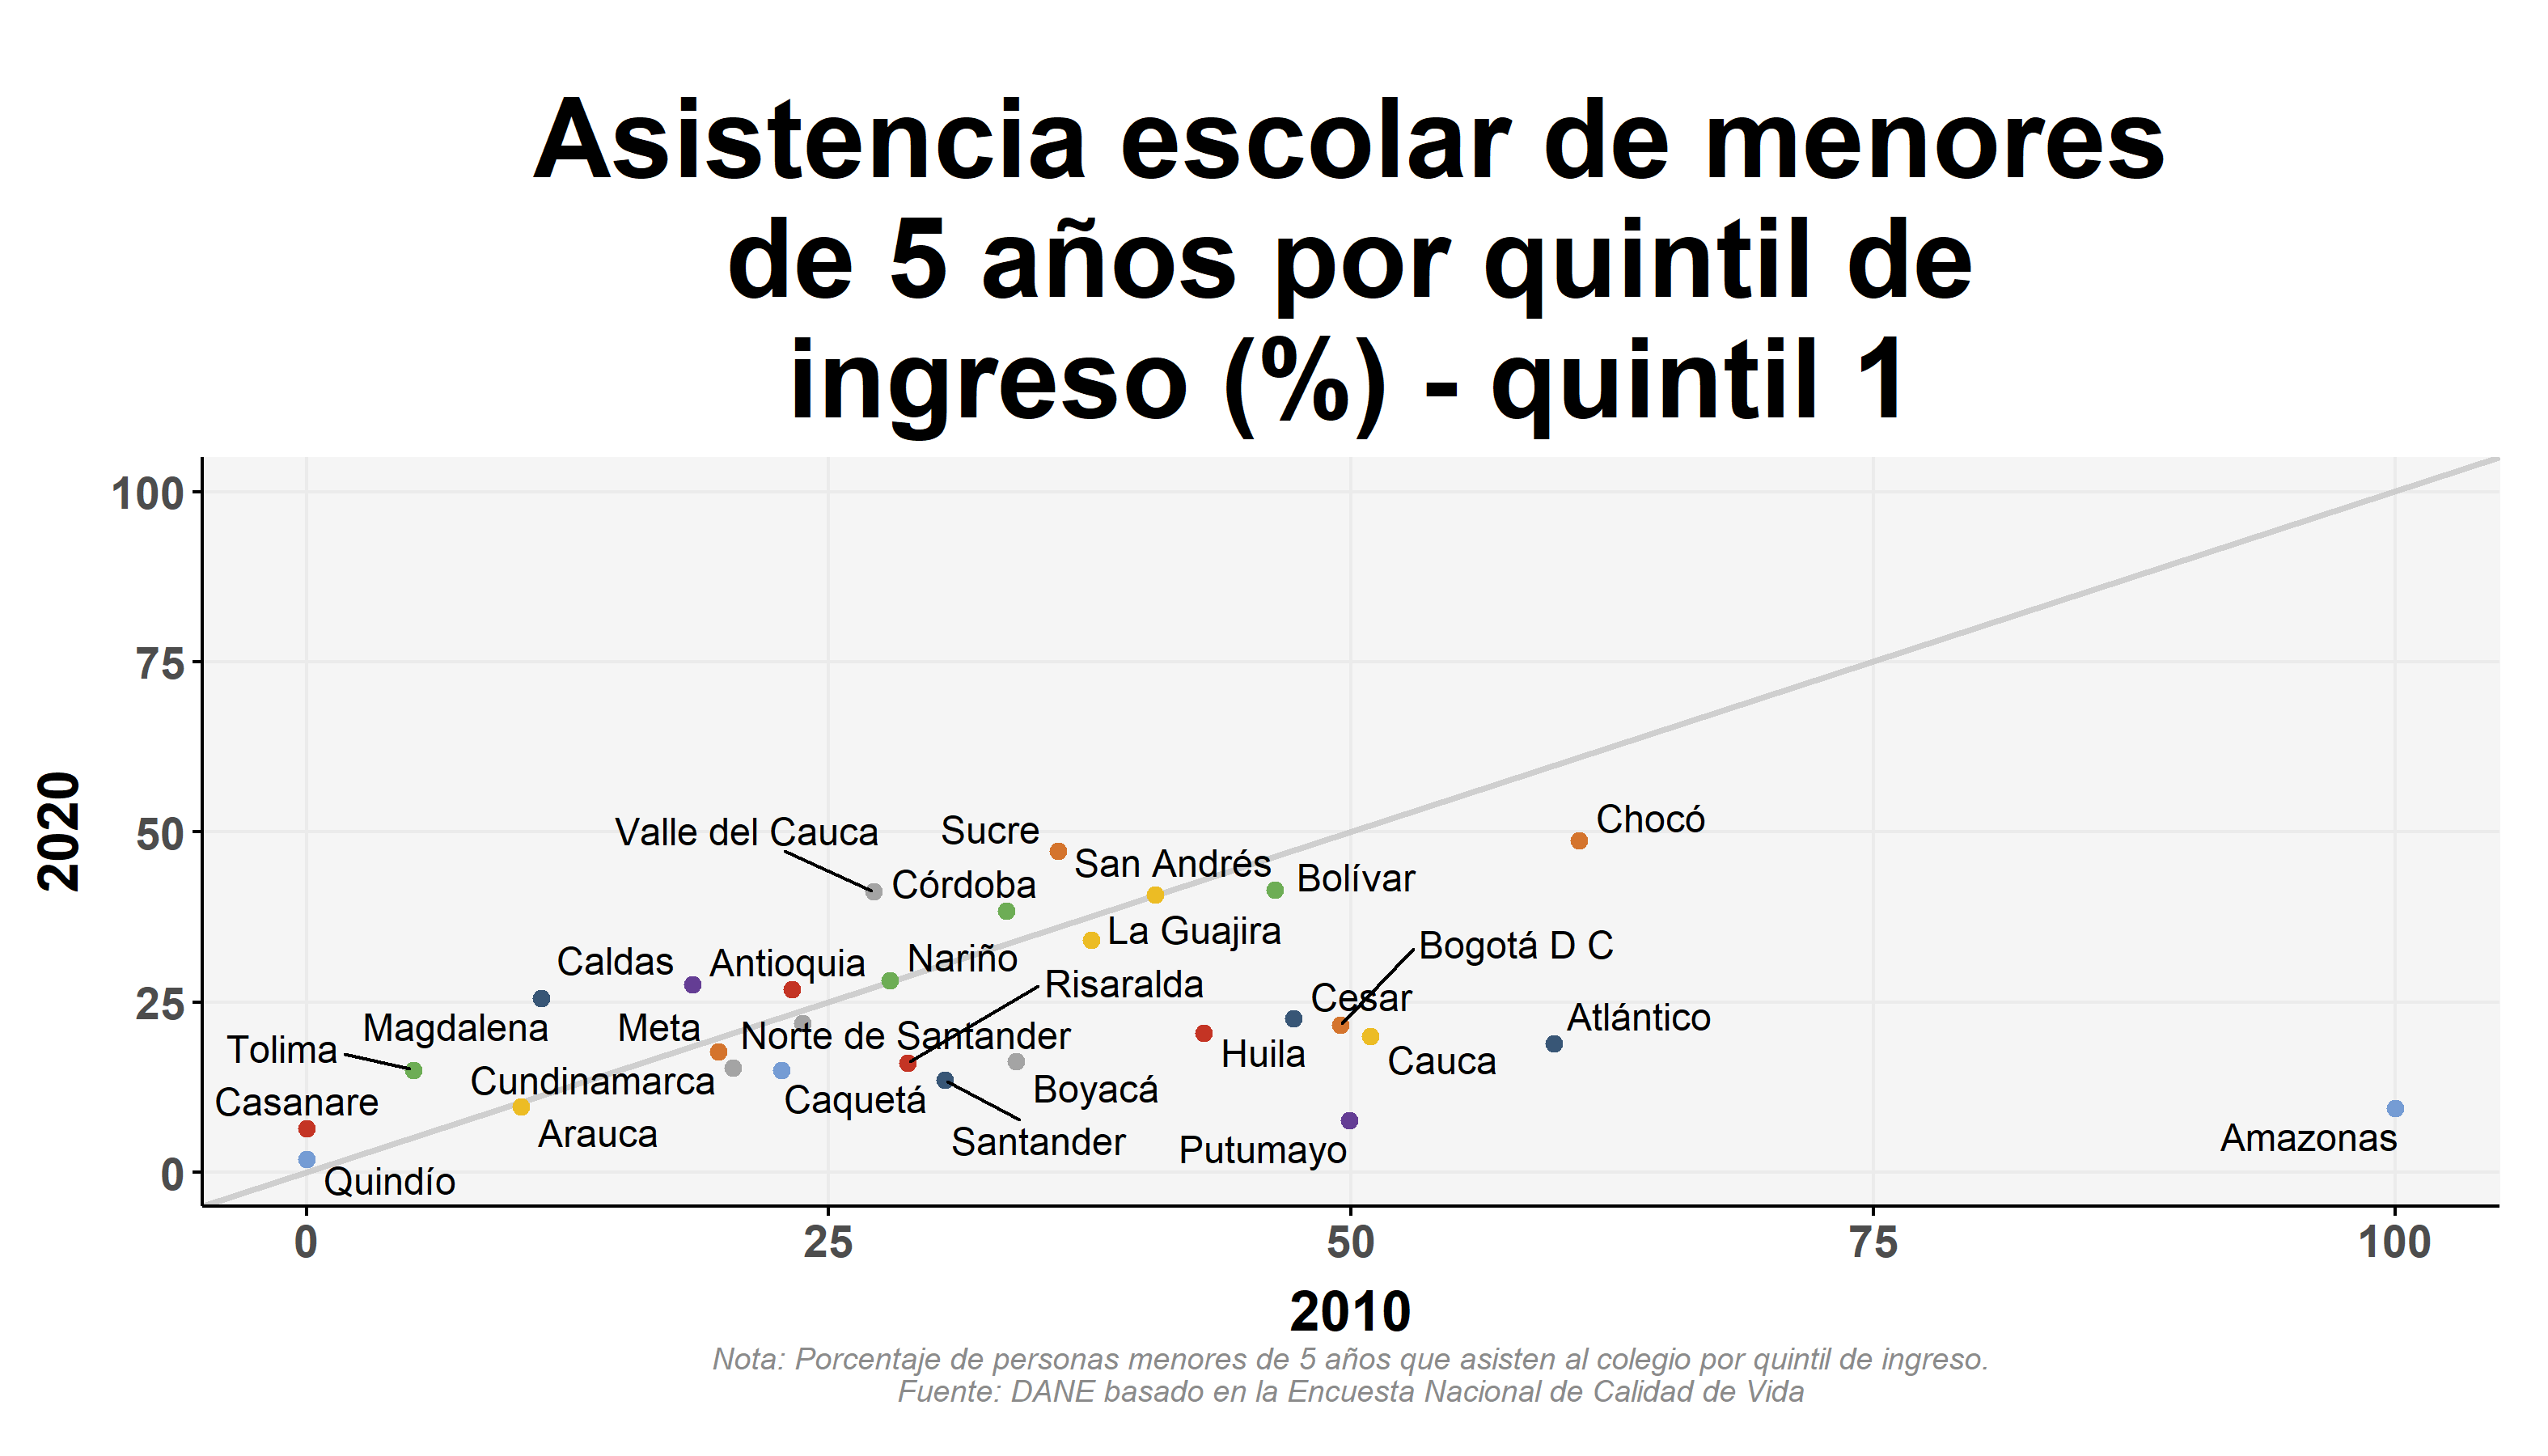
\includegraphics[width=\textwidth,keepaspectratio]{img/var_101_scatter_time.png}
        \end{center}
    \end{figure}
            \begin{itemize}
                \item Los dptos se concentran especialmente por debajo del 30\% de niños menores de 5 años asistiendo a un centro educativo en el primel quintil de ingresos.
                \item Gran parte de los dptos desmejoraron para 2020 la asistencia escolar de menores de 5 comparados con la información registrada para 2010.
                \item Valle, Tolima y Magdalena presentan son de los pocos dptos que presentaron mejoras en estos 10 años en el grupo de menor ingreso.
                \item Amazonas pasó de haber presentado una asistencia del 100\% en 2010 y ser el de mayor asistencia, a ser de los de menor asistencia con alrededor de un 10\%.
                \item San Andrés, Nariño, Meta y Cundinamarca se han mantenido en los niveles similares de hace 10 años.
                \end{itemize}

%%%% Include figures
    \begin{figure}[H]
        \caption{Asistencia escolar de menores de 5 años para el primer quintil de ingreso por departamentos para 2020 \label{map_result_2} }
        \begin{center}
        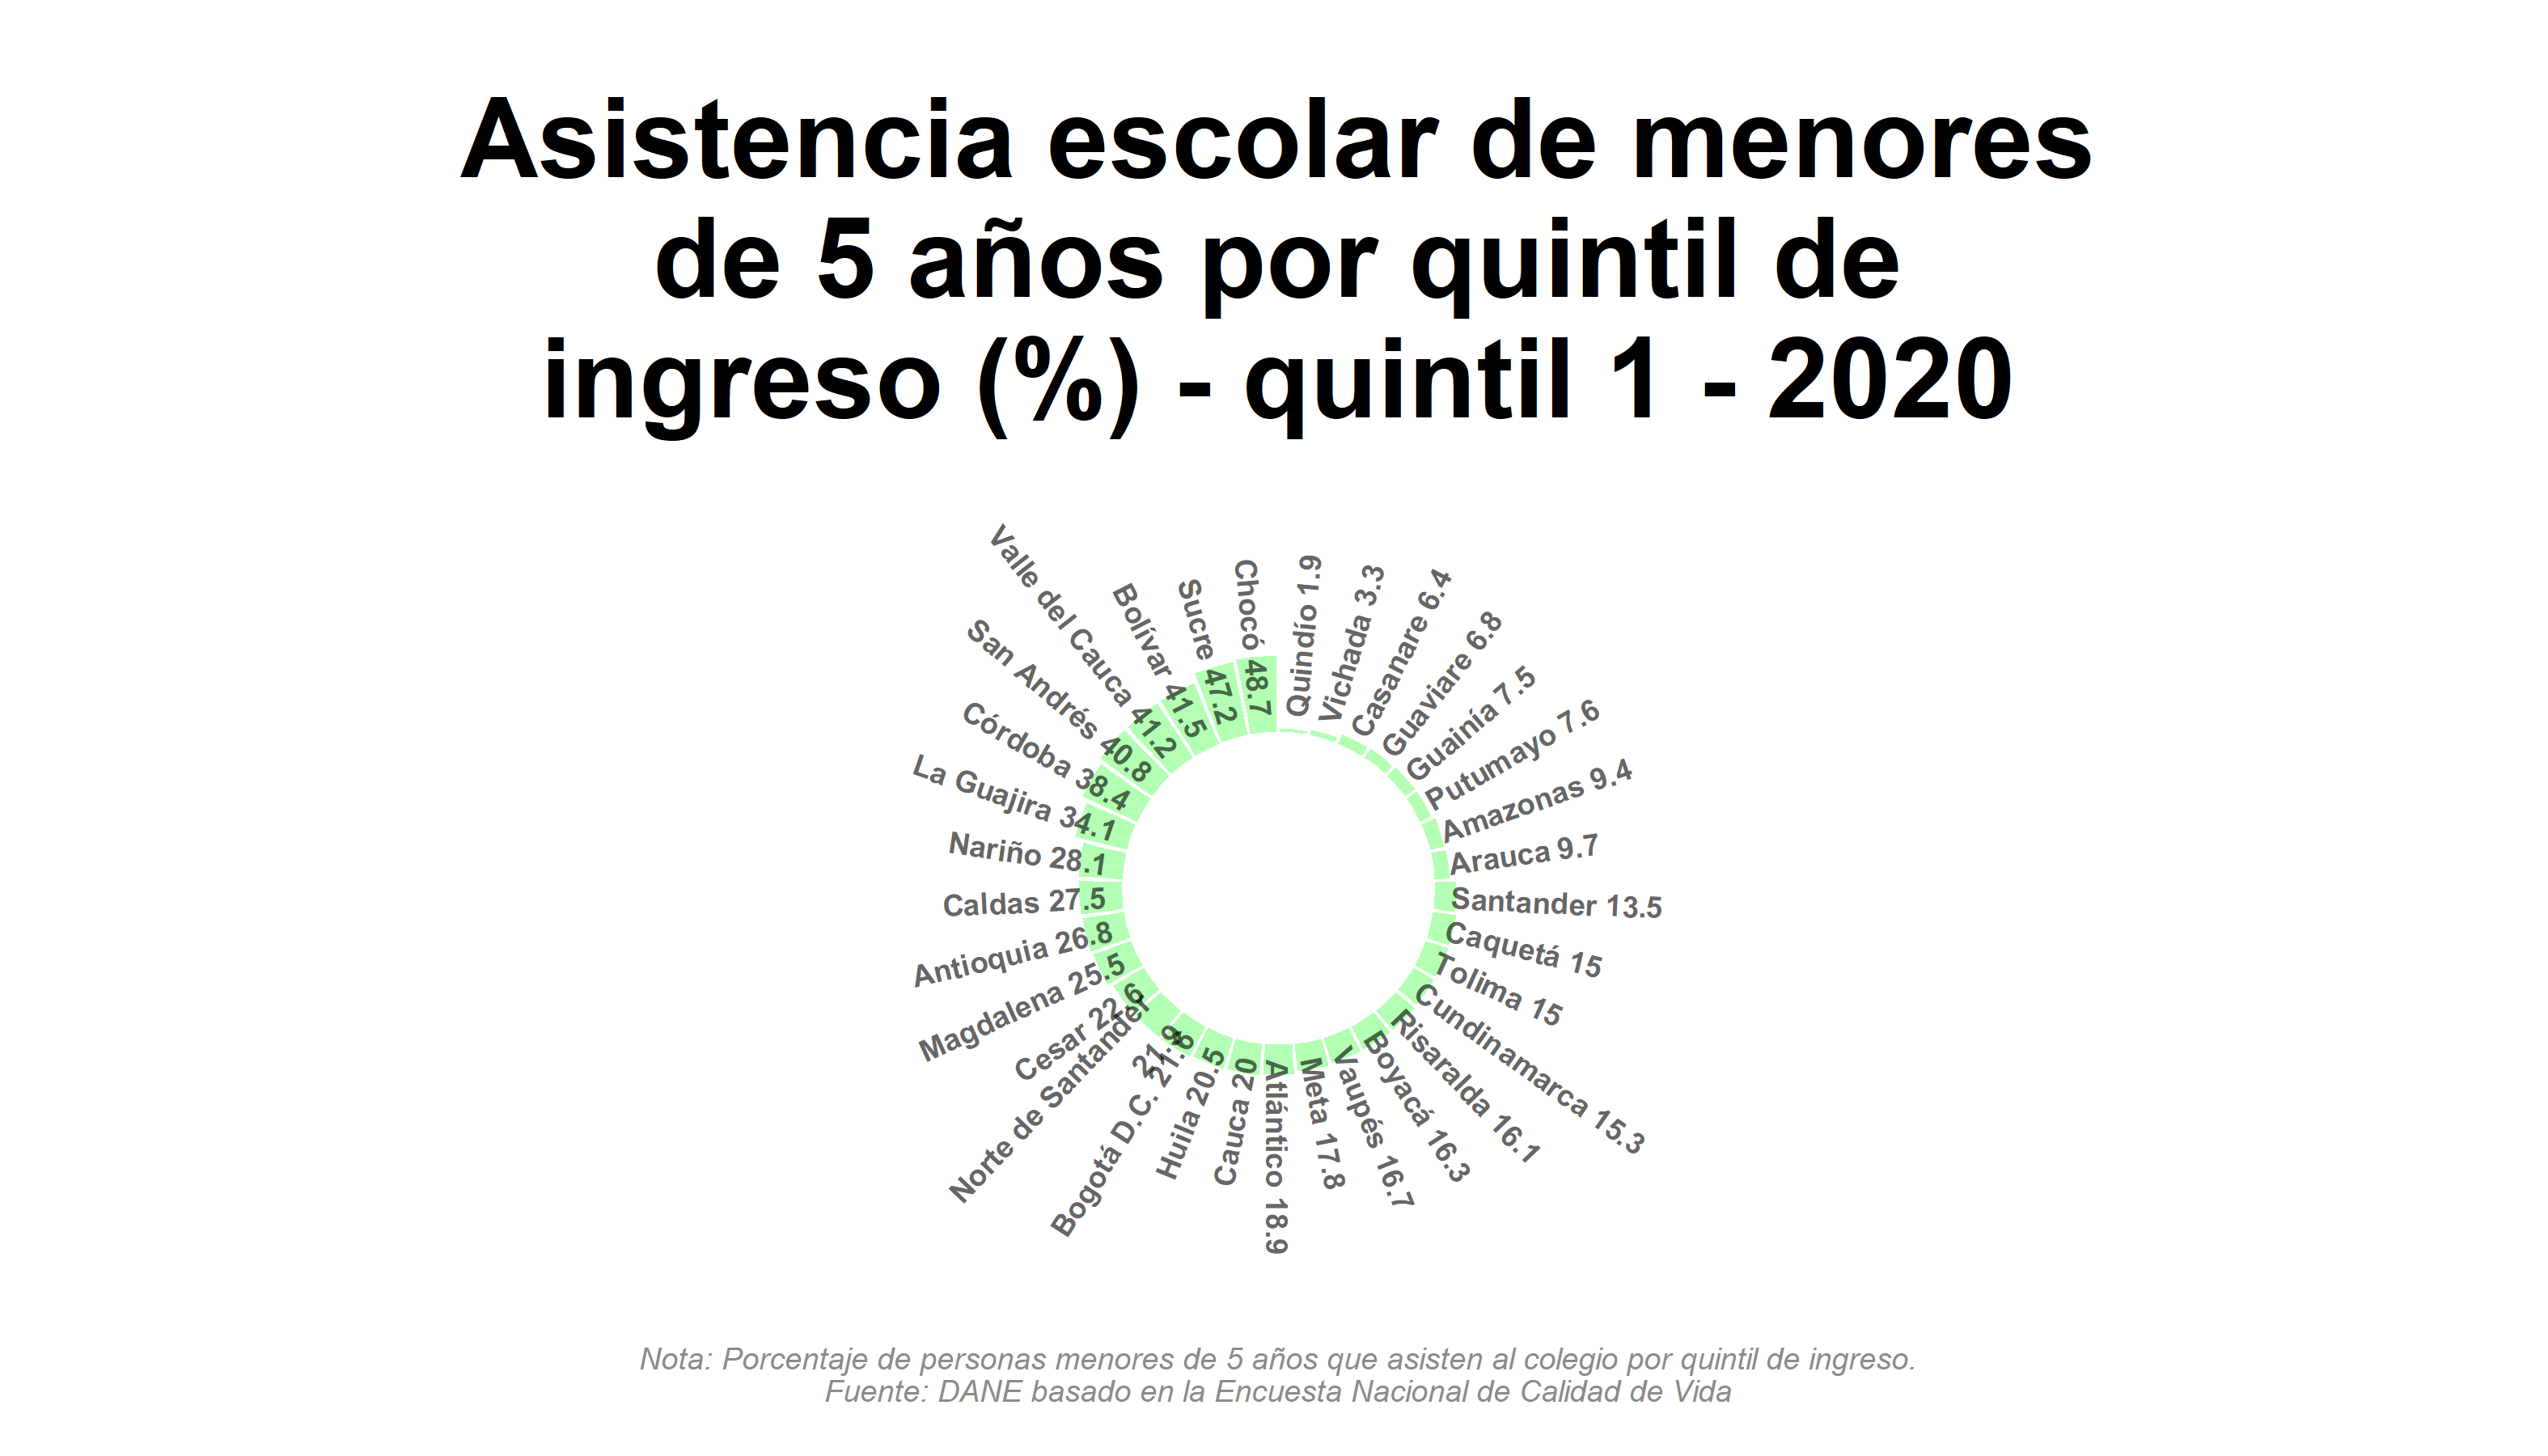
\includegraphics[width=\textwidth,keepaspectratio]{img/var_101_static.png}
        \end{center}
    \end{figure}
            \begin{itemize}
                \item Distribución heterogénea de los valores, abarcando desde el 3\% hasta cerca del 40\%.
                \item Mientras en el Quindío el porcentaje de menores de 5 que asisten a un centro educativo es de 1.9\%, el Chocó es de 48.7\% para el quintil de menor ingreso.
                \item Los dptos con menor asistencia escolar de menores de 5 se encuentran en la zona amazónica y oriental.
                \end{itemize}

%%%% Include figures
    \begin{figure}[H]
        \caption{Asistencia escolar de menores de 5 años para el primer quintil de ingreso por zonas \label{map_result_2} }
        \begin{center}
        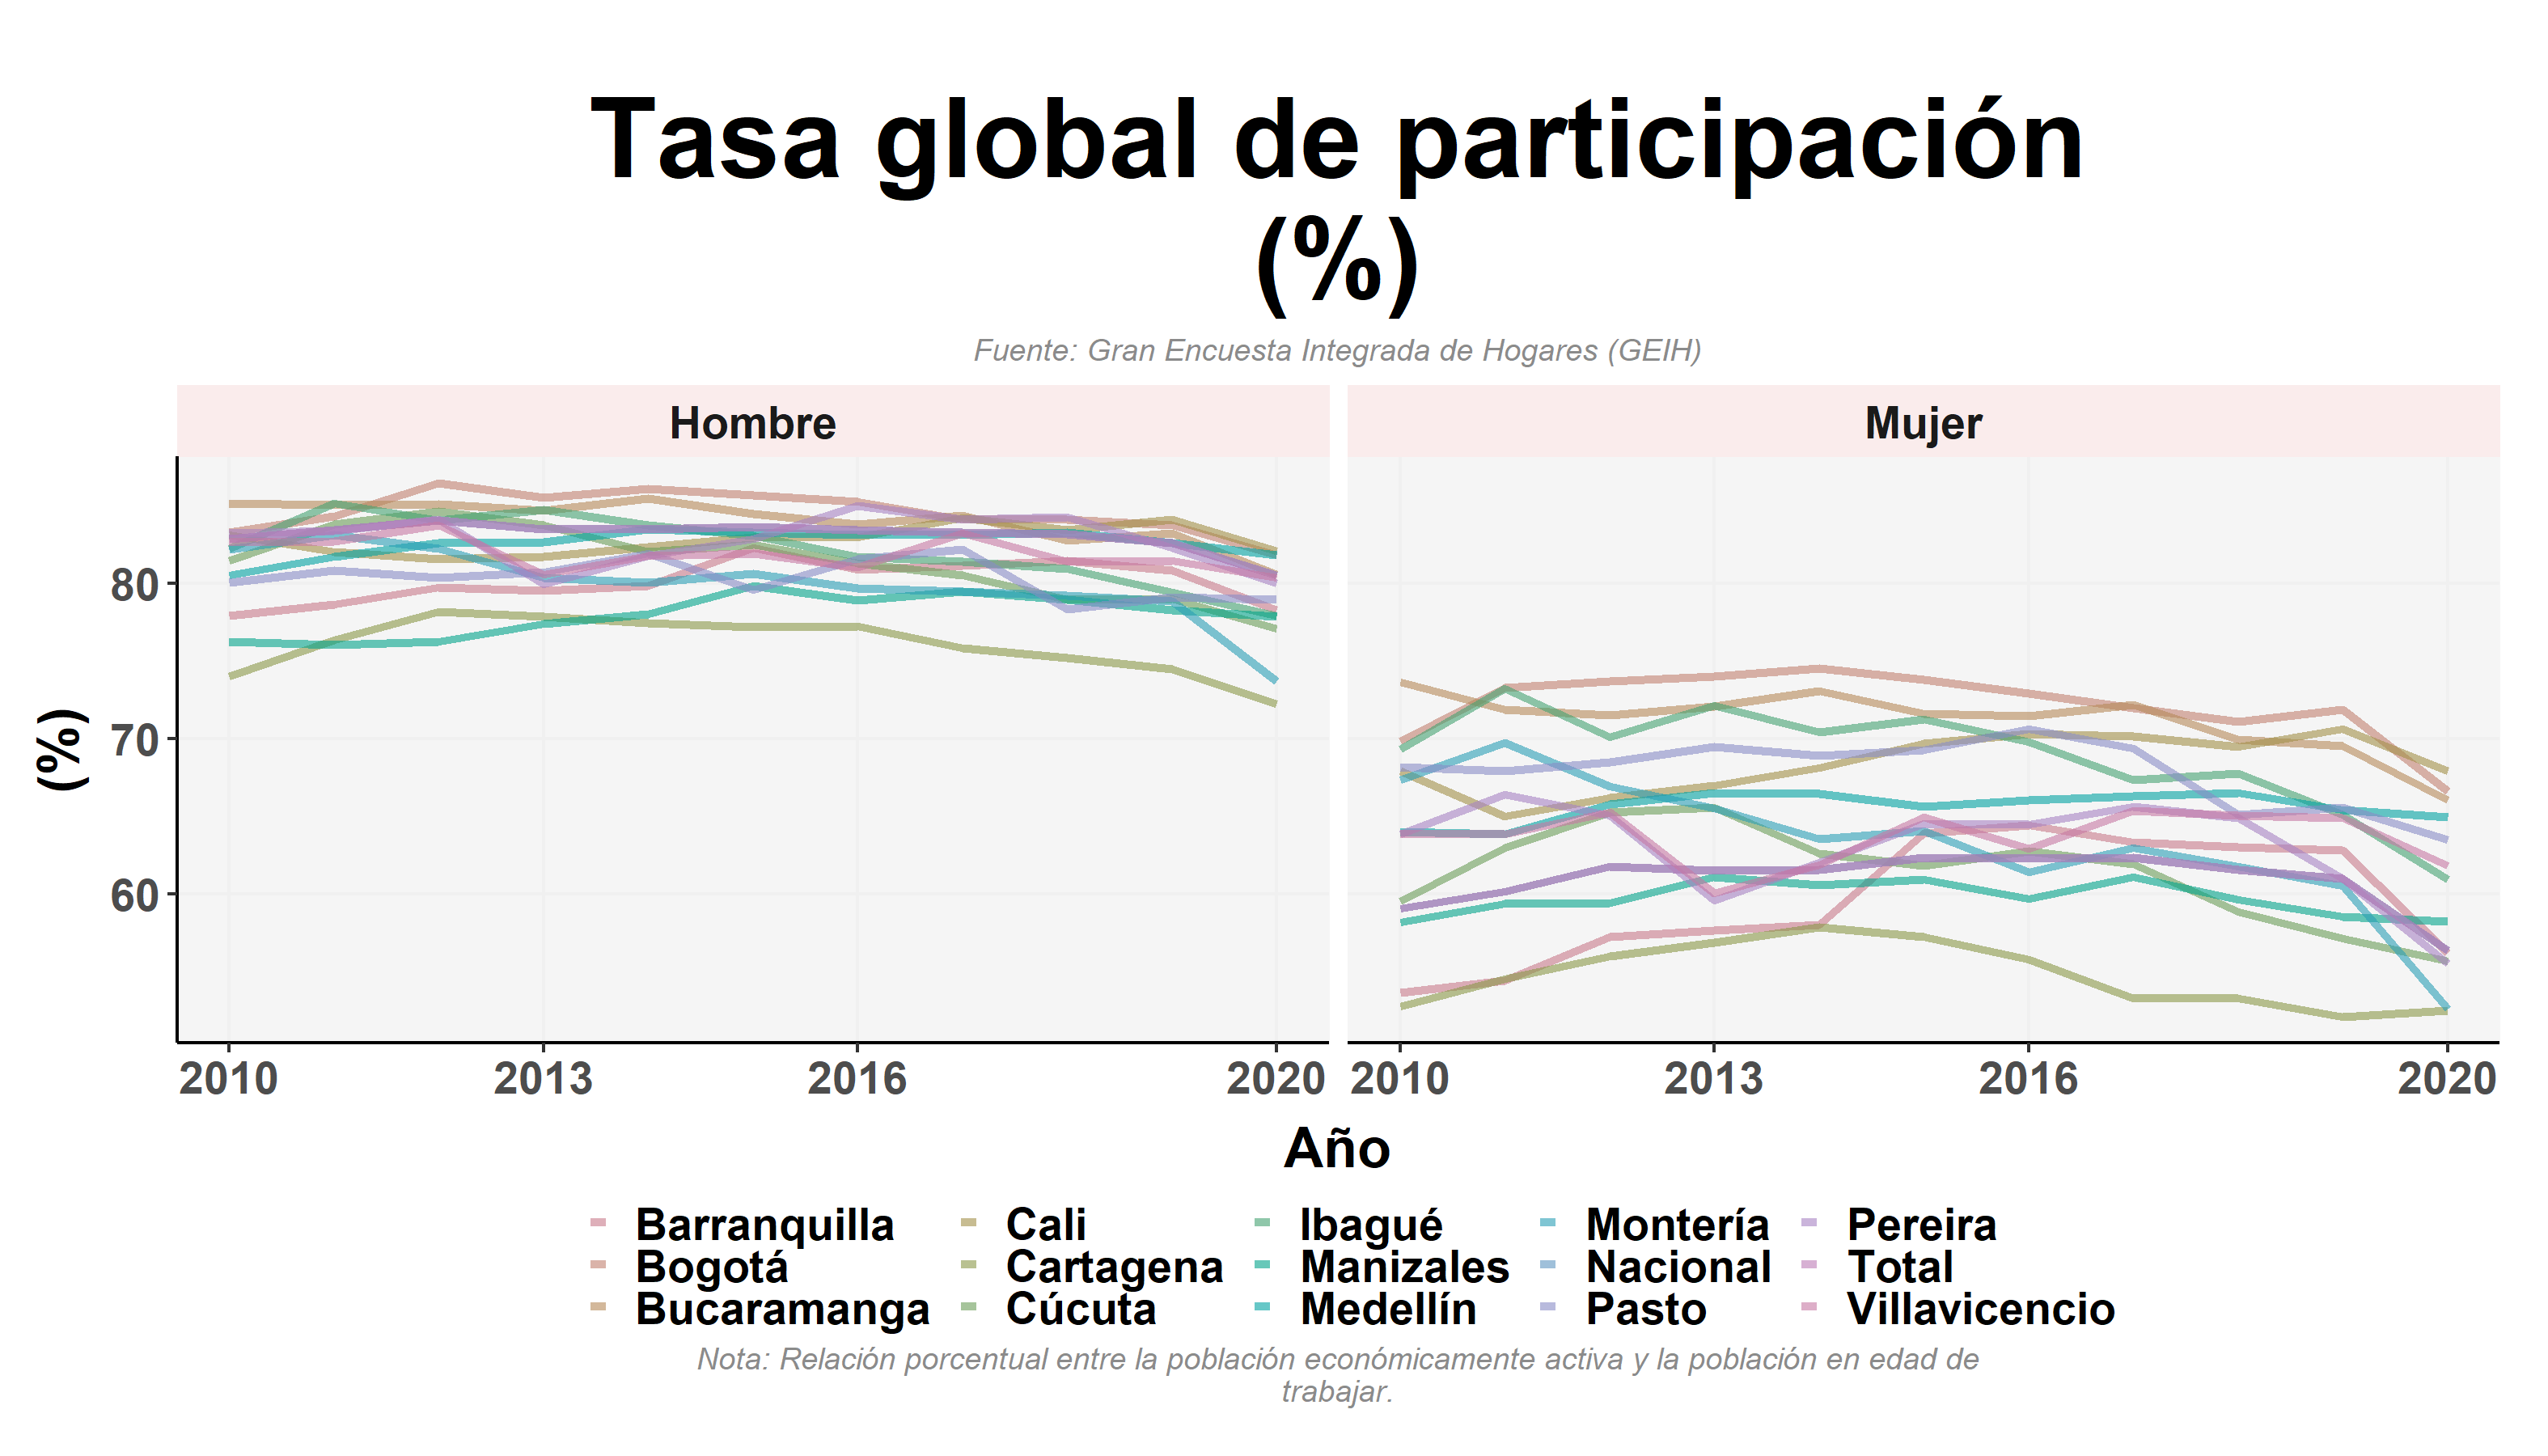
\includegraphics[width=\textwidth,keepaspectratio]{img/var_102_trend.png}
        \end{center}
    \end{figure}
            \begin{itemize}
                \item En el primer quintil de ingreso se ve que la asistencia escolar en menores de 5 años es mayor en las cabeceras, casi siendo el doble de las zonas rurales.
                \item En las cabeceras se evidenciaba un aumento en la asistencia escolar hasta el 2017, donde inicia a decaer, especialmente en 2020 donde es bastante pronunciada, estando en los niveles más bajos desde el 2010.
                \item En el caso de las zonas rurales esta se mantuvo estables entre 2016 y 2019 decayendo para 2020 y teniendo menor asistencia a la registrada en 2010.
                \item La brecha entre las zonas se mantuvo hasta 2020, donde esta disminuyó a una diferencias alrededor del 10\%.
                \end{itemize}

        \subsubsection{PENDIENTE - Asistencia escolar a educación primaria}
        
    \subsection{Calidad de la educación}
        \subsubsection{Tamaño de clase en primaria}

%%%% Include figures
    \begin{figure}[H]
        \caption{Tamaño de clase en primaria por departamentos - 2010 VS 2020 \label{map_result_2} }
        \begin{center}
        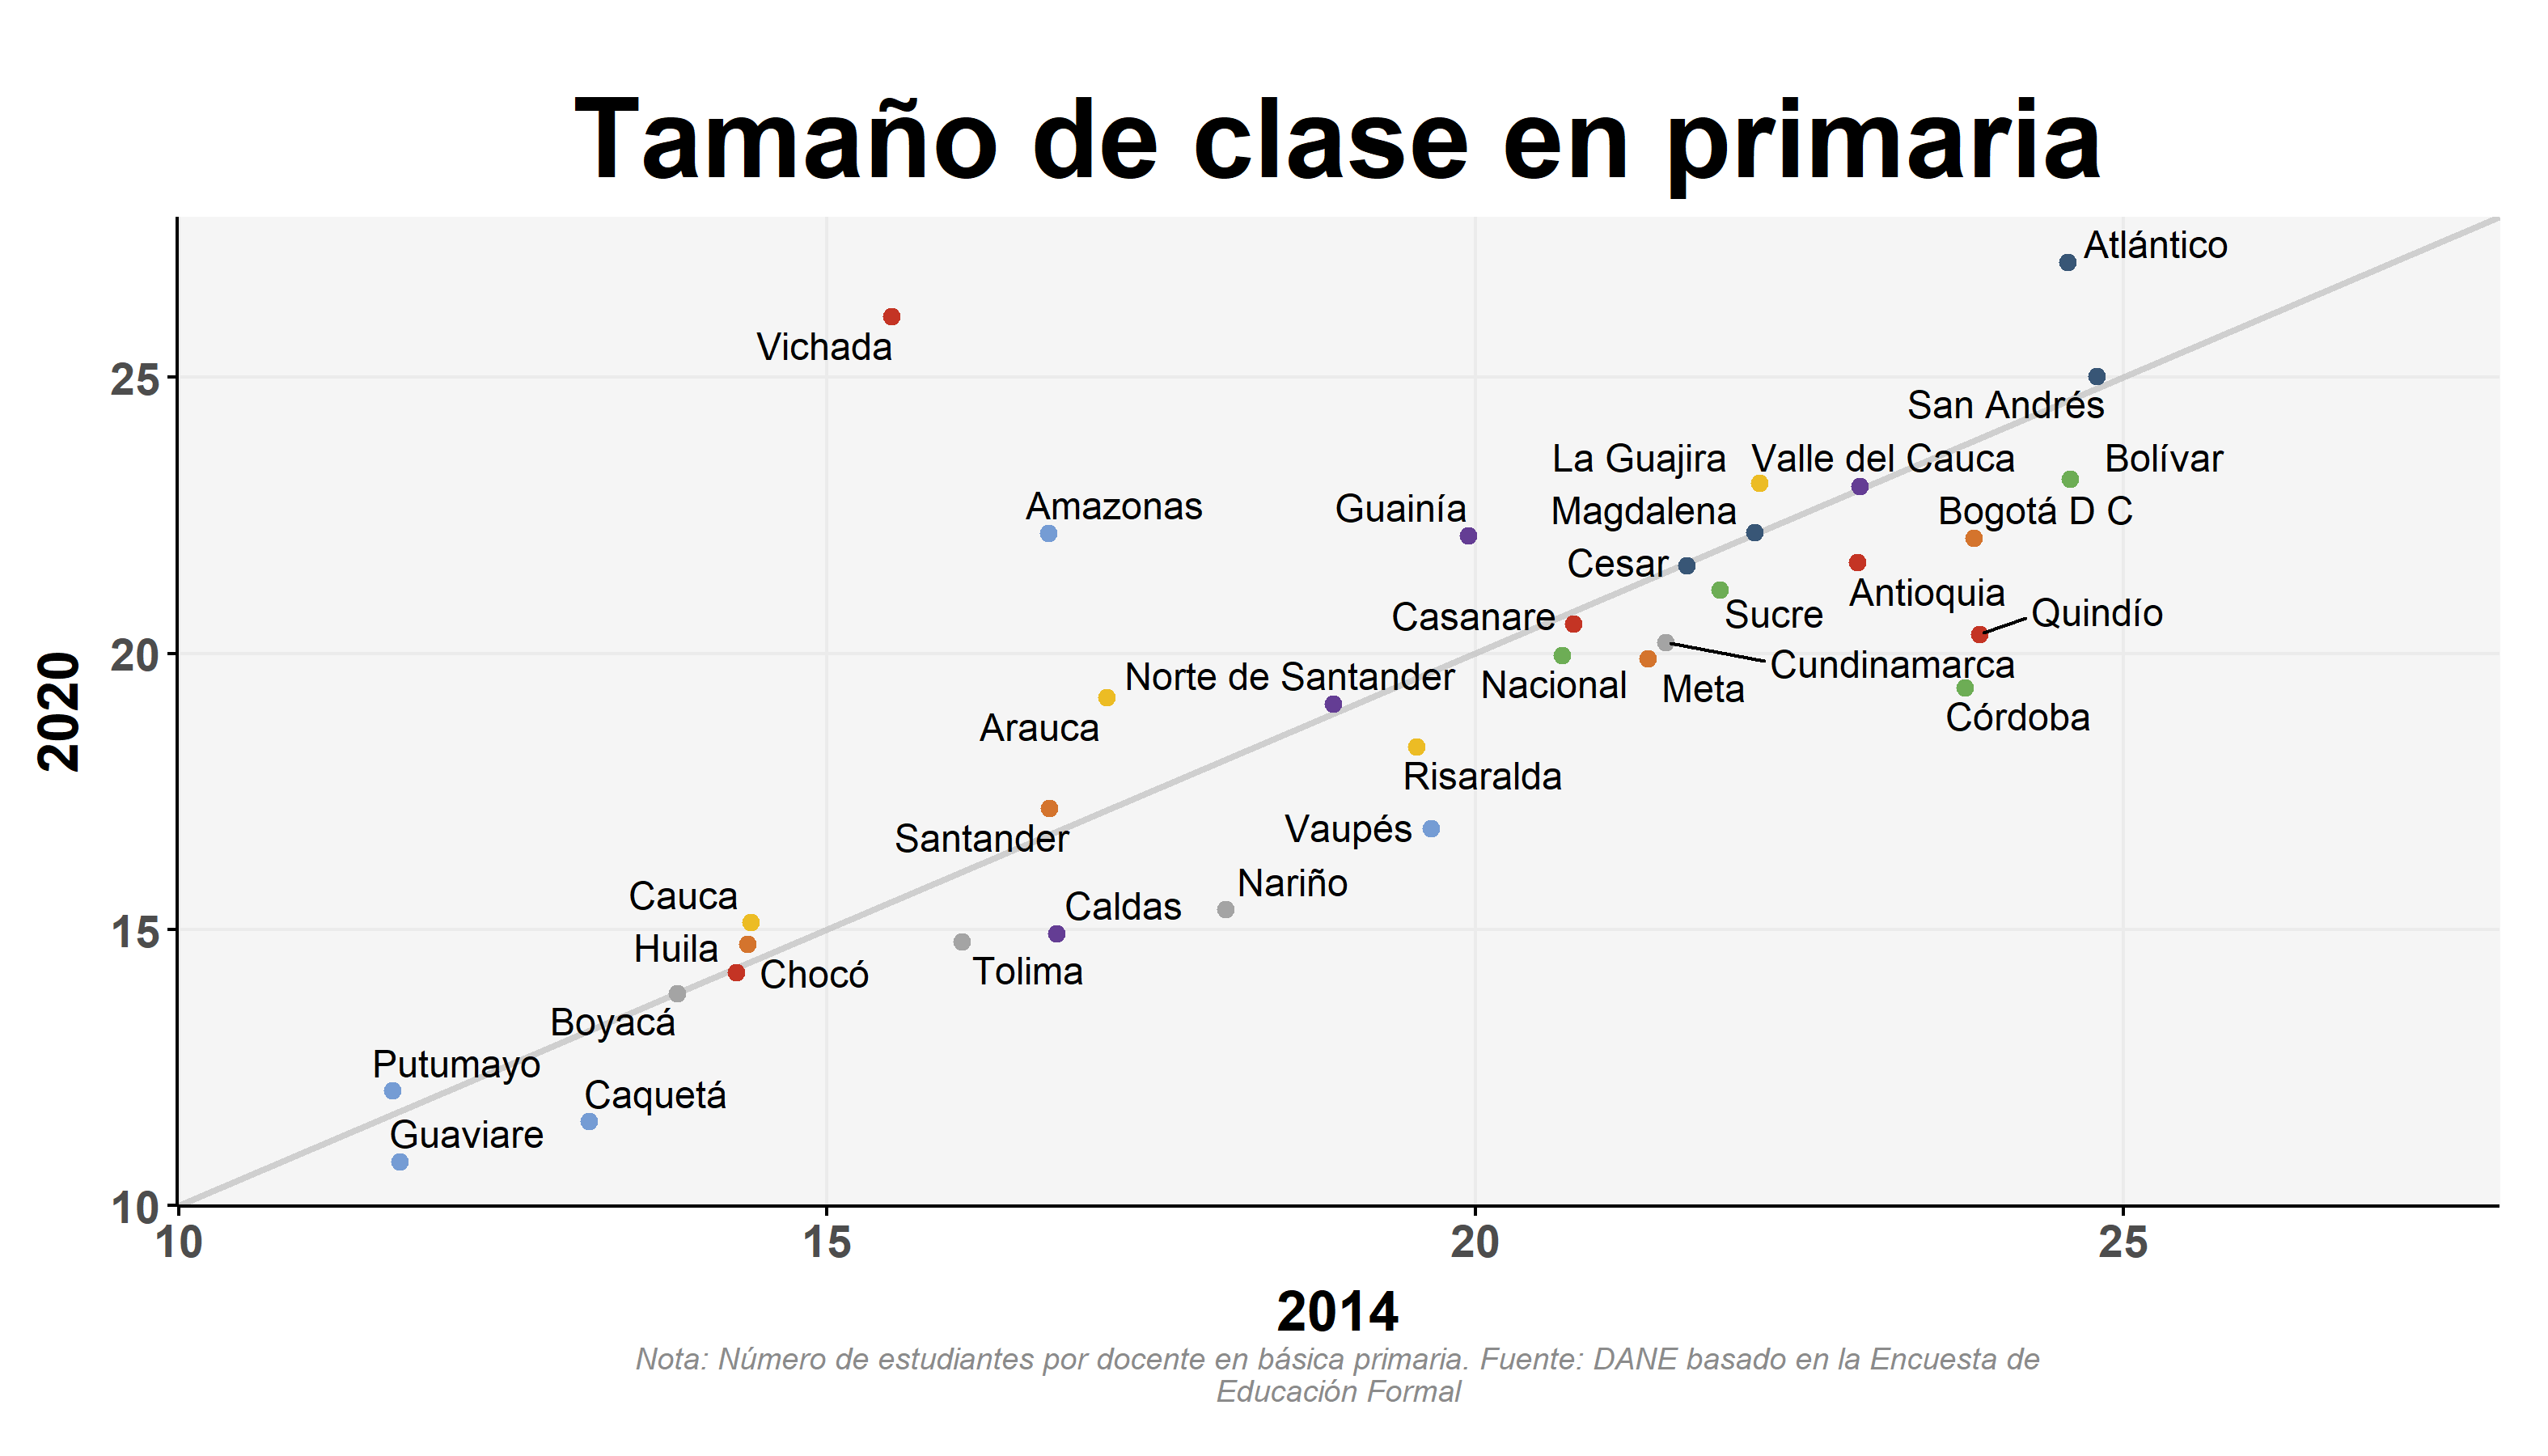
\includegraphics[width=\textwidth,keepaspectratio]{img/var_228_scatter_time.png}
        \end{center}
    \end{figure}
            \begin{itemize}
                \item En general los departamentos han disminuido o mantenido levemente el número de estudiantes por docente en primaria entre 2014 y 2020.
                \item Vichada ha sido de los que presentó un mayor aumento, pasando de estar cerca de 15 estudiantes por docente a 25, de igual manera Amazonas paso de aproximadamente 17 a 22 estudiantes por docente.
                \item Vichada pasó de estar entre los diez con menor tamaño de clase en primaria, a ser el segundo con más estudiantes por docente.
                \end{itemize}

%%%% Include figures
    \begin{figure}[H]
        \caption{Tamaño de clase en primaria por departamentos para 2020 \label{map_result_2} }
        \begin{center}
        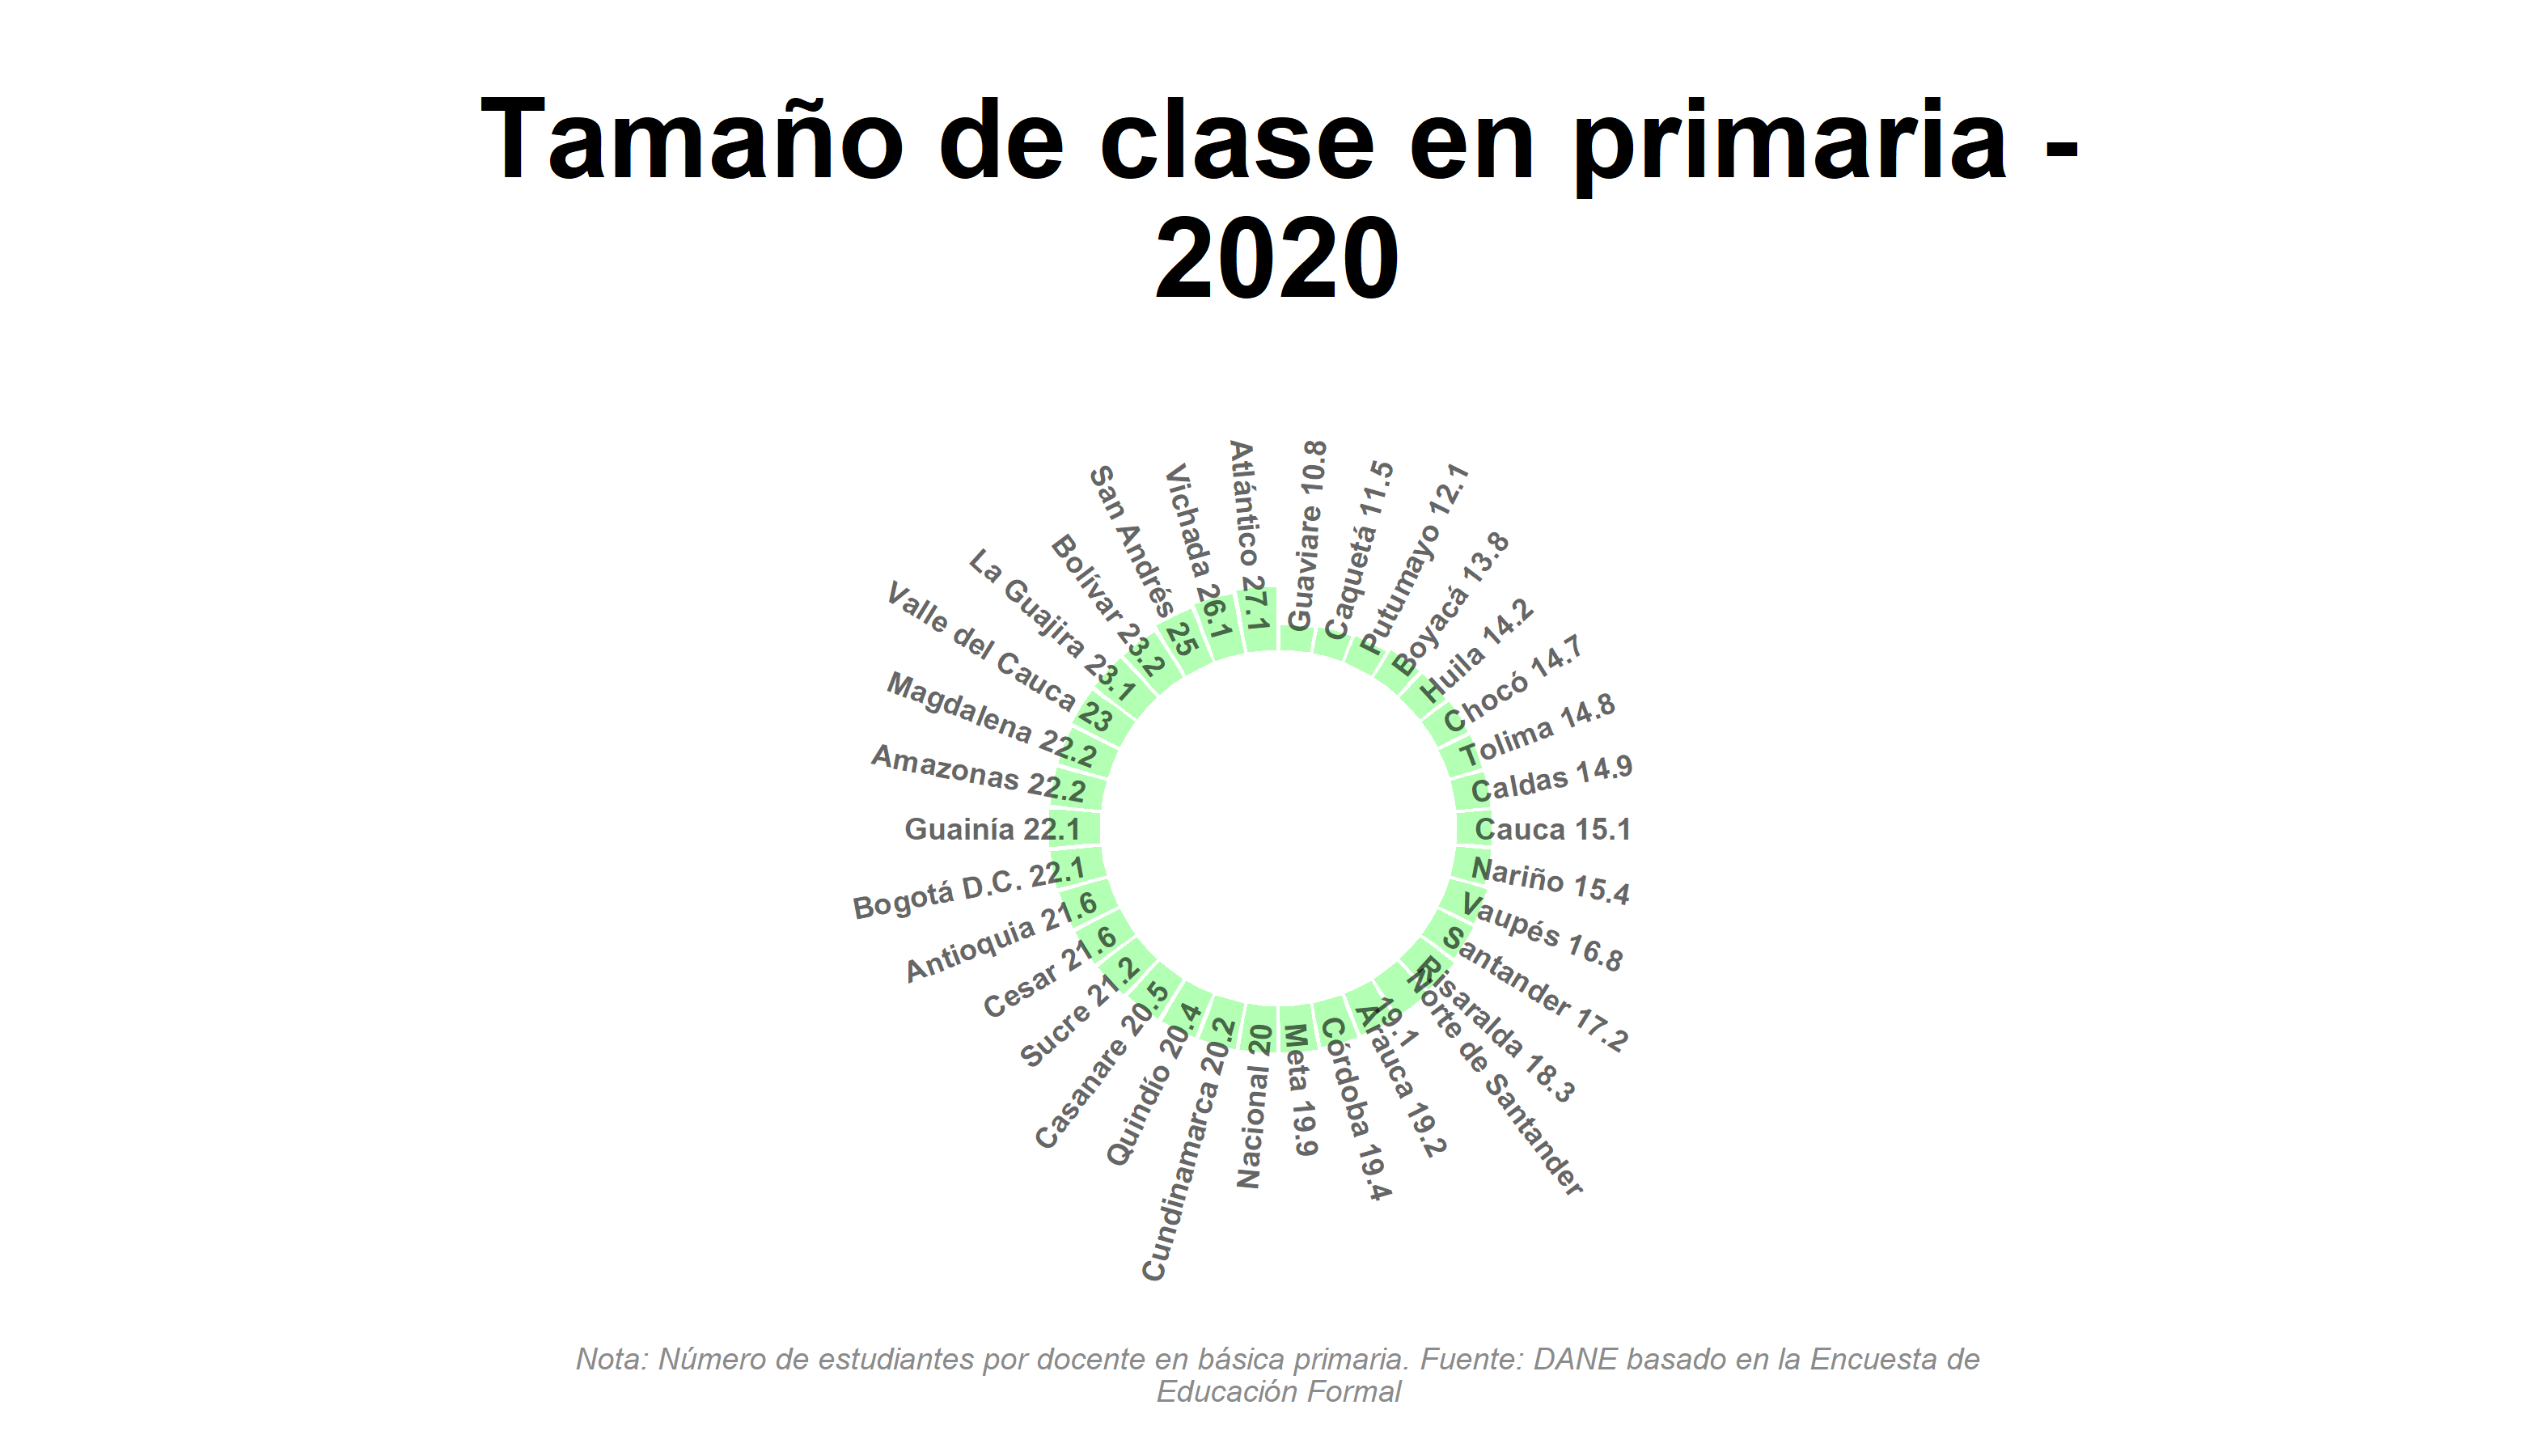
\includegraphics[width=\textwidth,keepaspectratio]{img/var_228_static.png}
        \end{center}
    \end{figure}
            \begin{itemize}
                \item Hay una diferencia de aproximadamente 17 estudiantes entre el tamaño de clase en Atlántico y Vichada, siendo el de mayor y menor tamaño en promedio respectivamente.
                \item Los dptos con mayor tamaño en las clases en primario se concentran especialmente en la costa Caribe colombiana.
                \item En el centro-sur del país se concentran los dptos con menor tamaño de clase (228 map 2020).
                \end{itemize}

%%%% Include figures
    \begin{figure}[H]
        \caption{Tamaño de clase en primaria a nivel nacional \label{map_result_2} }
        \begin{center}
        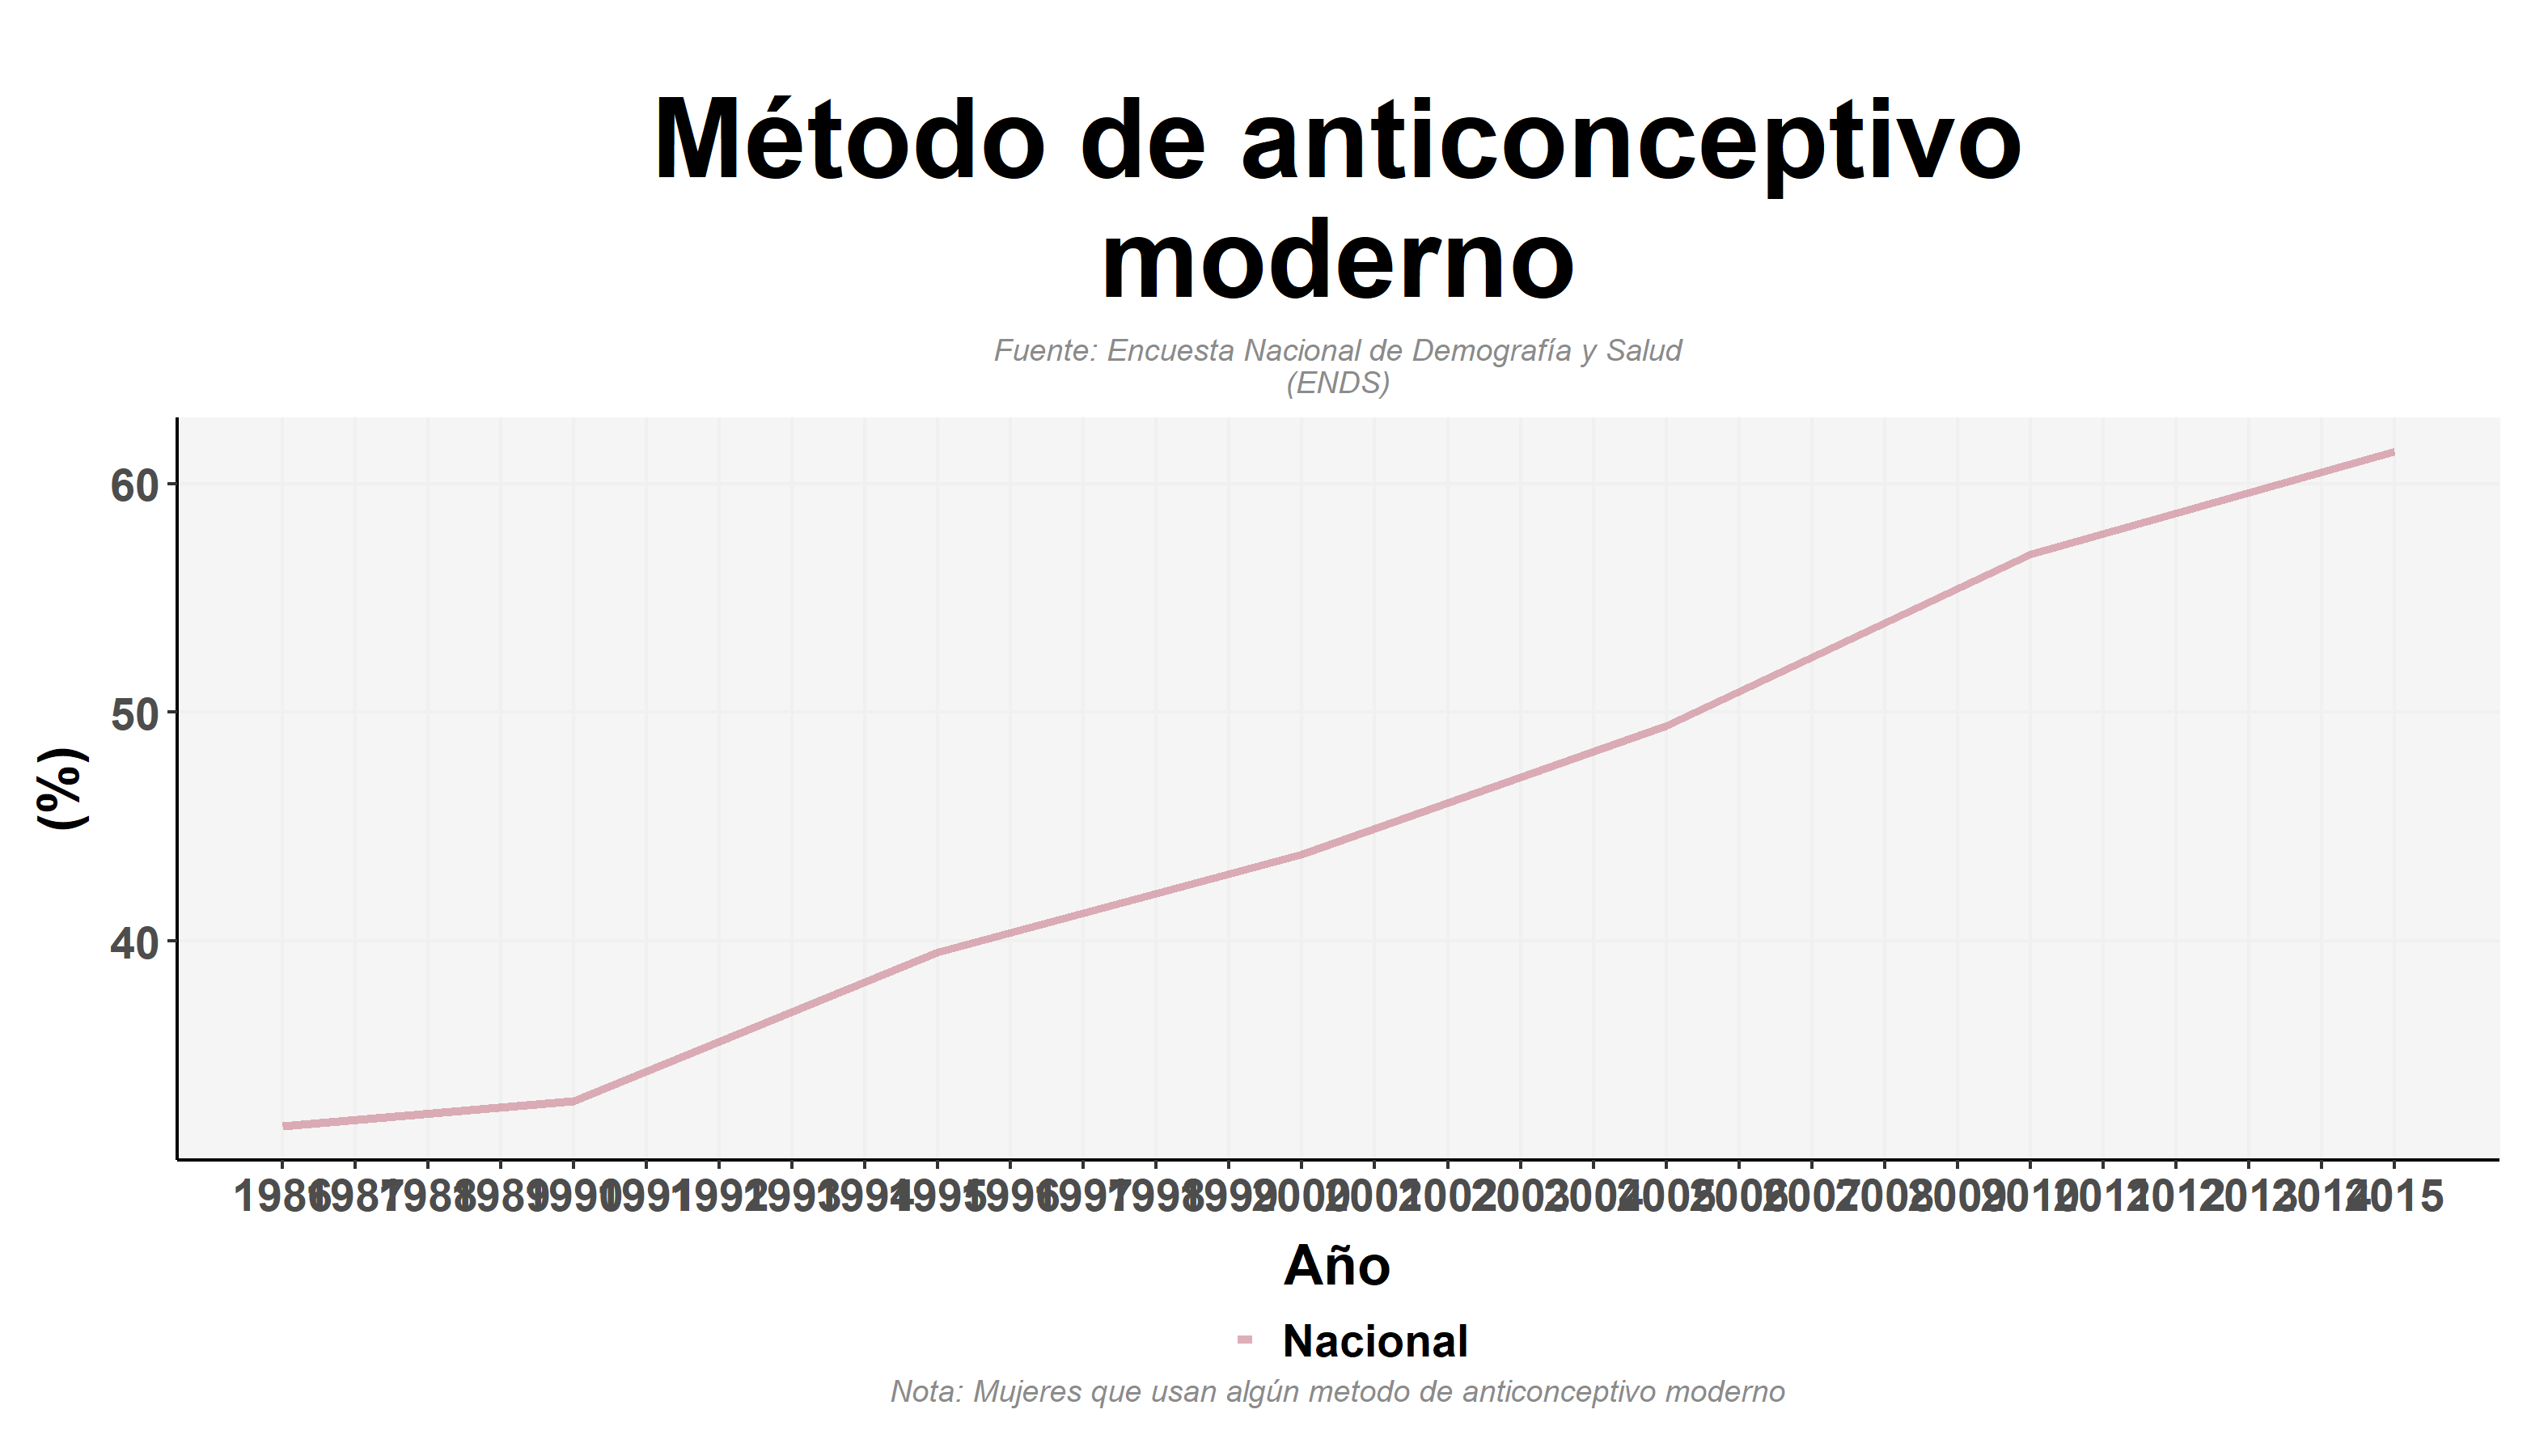
\includegraphics[width=\textwidth,keepaspectratio]{img/var_229_trend.png}
        \end{center}
    \end{figure}
            \begin{itemize}
                \item El tamaño de clase ha venido disminuyendo significativamente desde el 2014.
                \item En 2016 hubo un aumento en el tamaño de la clase, pero se compensó al año siguiente.
                \item Los últimos tres años a mantenido niveles del 20 estudiantes por docente.
                \end{itemize}

\section{Juventud}
    \subsection{Educación superior}

%%%% Include figures
    \begin{figure}[H]
        \caption{Jóvenes de 18 a 28 años que han asistido a una institución de educación superior por departamentos - 2010 VS 2020 \label{map_result_2} }
        \begin{center}
        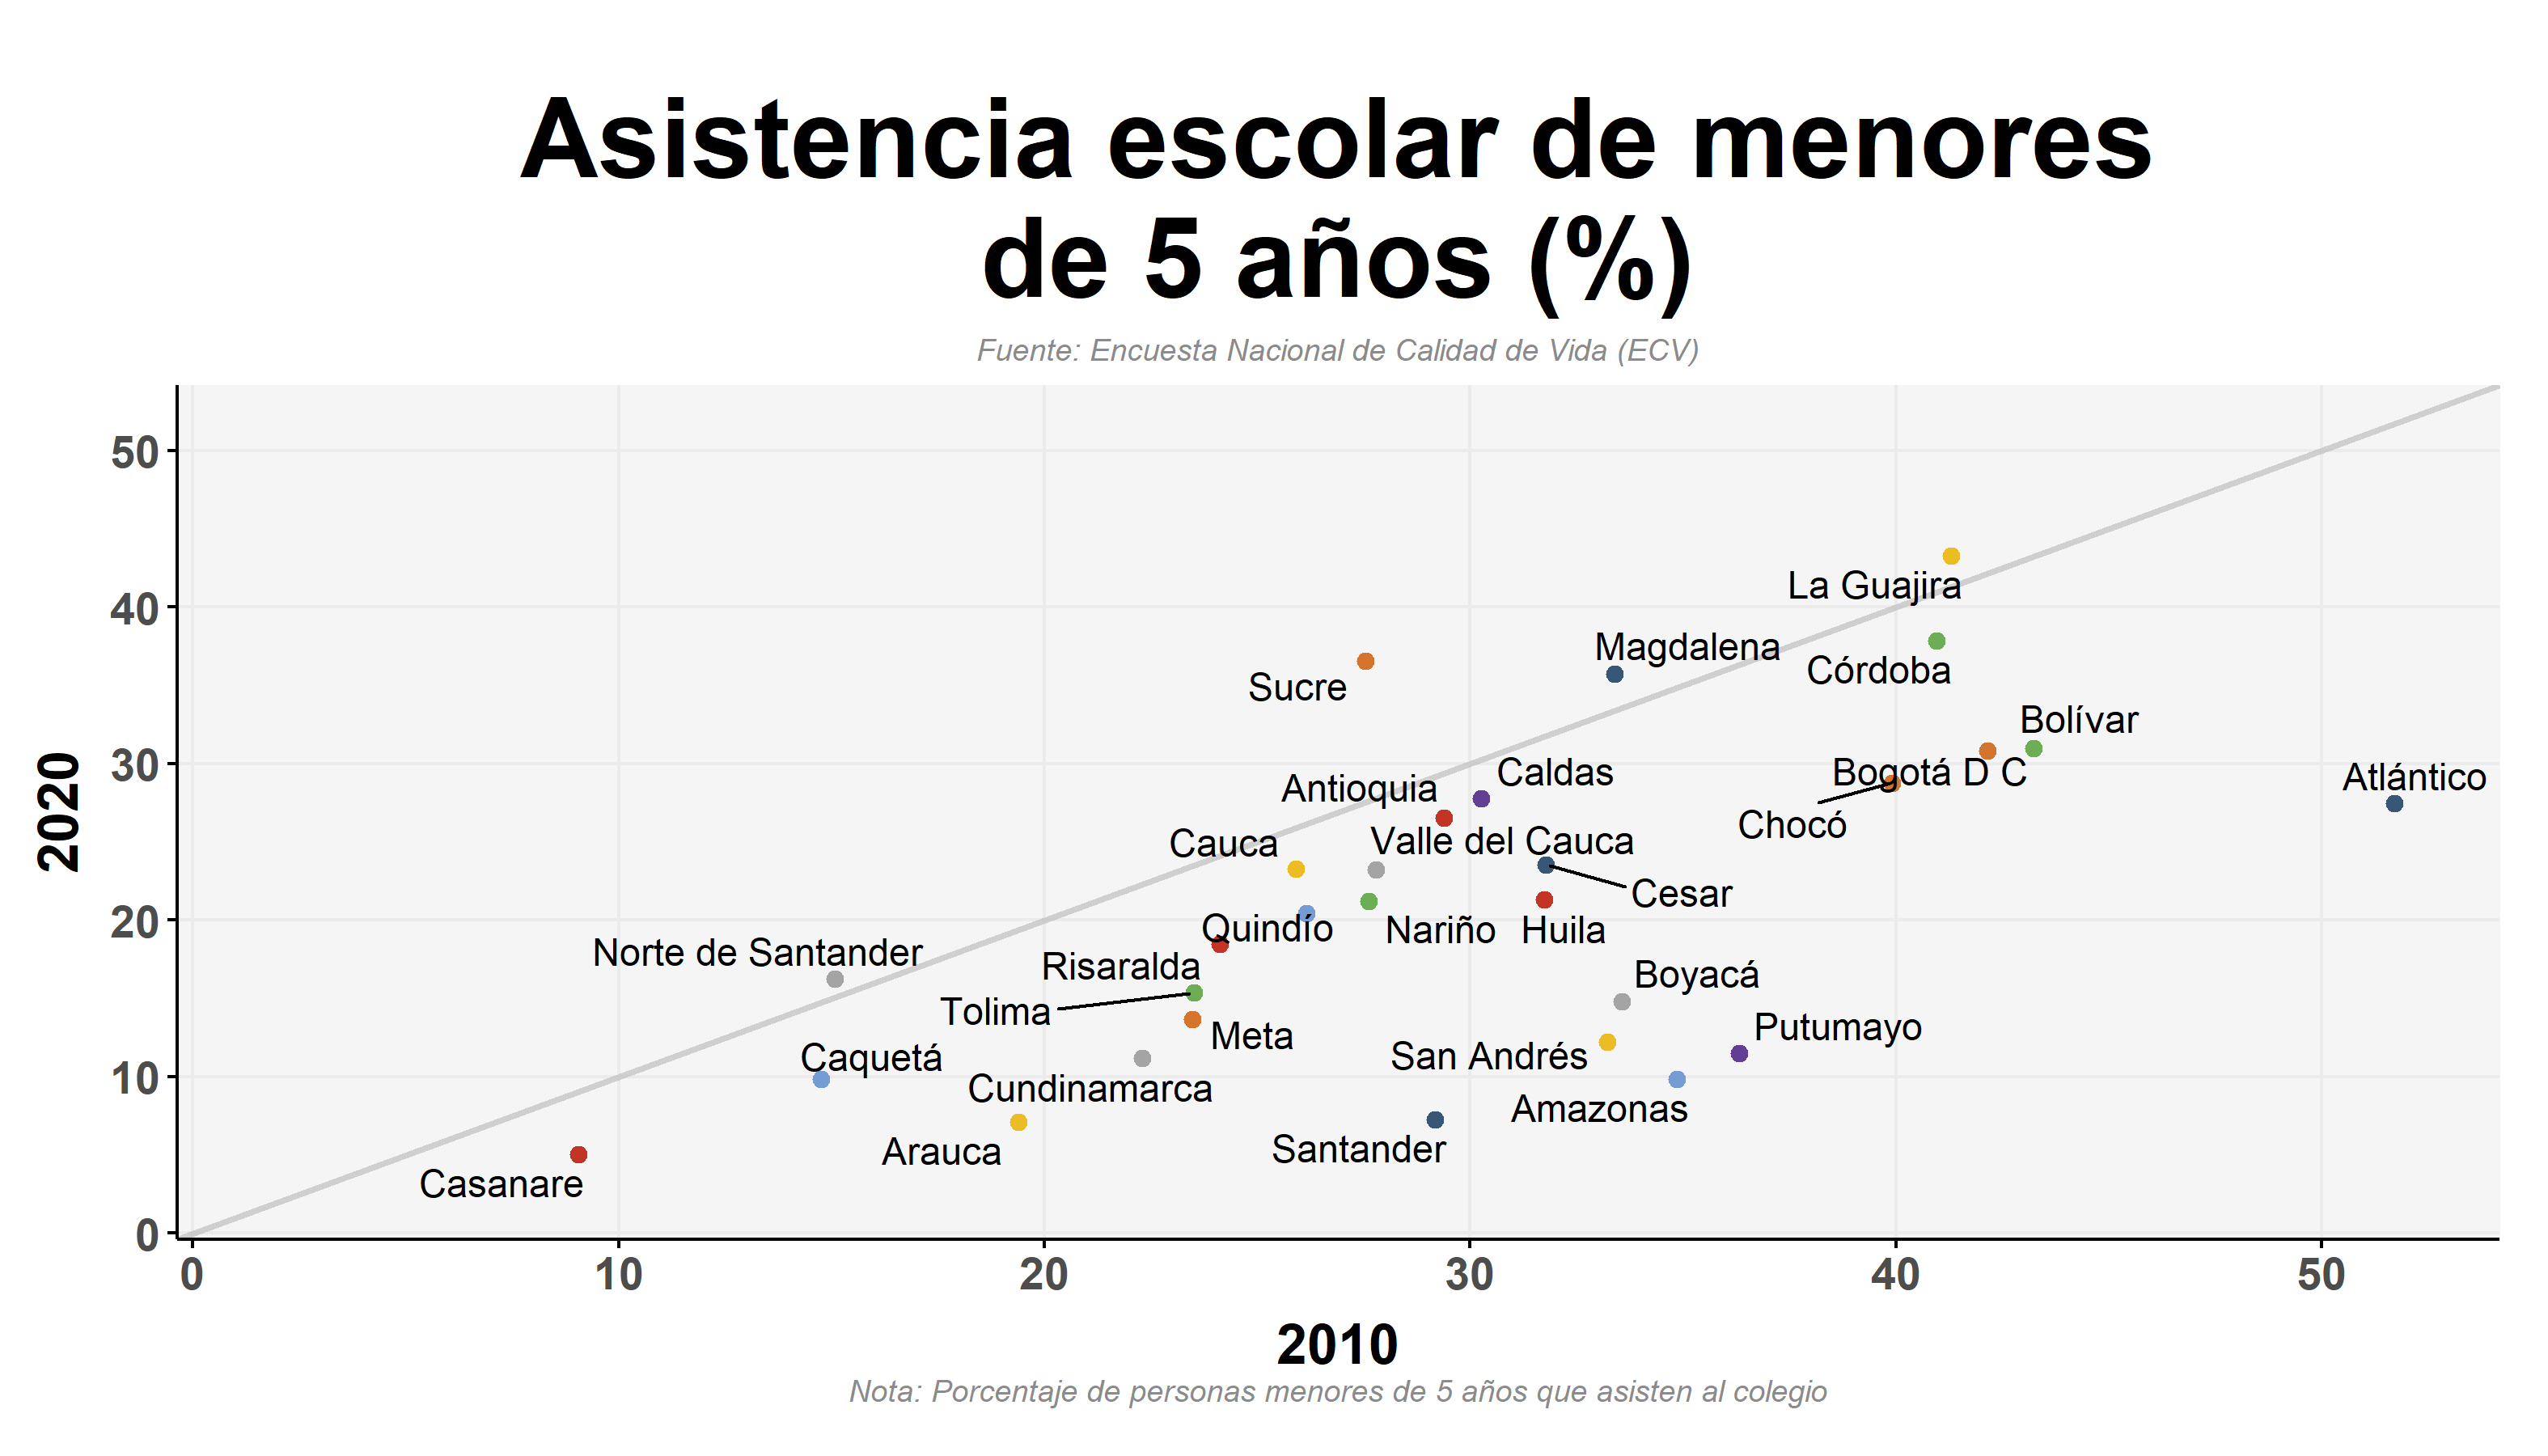
\includegraphics[width=\textwidth,keepaspectratio]{img/var_127_scatter_time.png}
        \end{center}
    \end{figure}
            \begin{itemize}
                \item Boyacá, Arauca y Amazonas presentaron una disminución fuerte en el \% de jóvenes que han asistido a la educación superior, siendo el primero el de mayor disminución pasando de estar cerca del 50\% a estar debajo del 30\%. Los otros dos pasaron de estar cerca al 30\% a valores cercanos a 15 y 10\% respectivamente.
                \item Caquetá, Risaralda, Caldas, Cundinamarca, Córdoba y Magdalena presentan el mayor aumento, alrededor del doble para 2020, comparado con lo reportado en 2010 (gráfica map change 127).
                \end{itemize}

%%%% Include figures
    \begin{figure}[H]
        \caption{Jóvenes de 18 a 28 años que han asistido a una institución de educación superior por departamentos para 2020 \label{map_result_2} }
        \begin{center}
        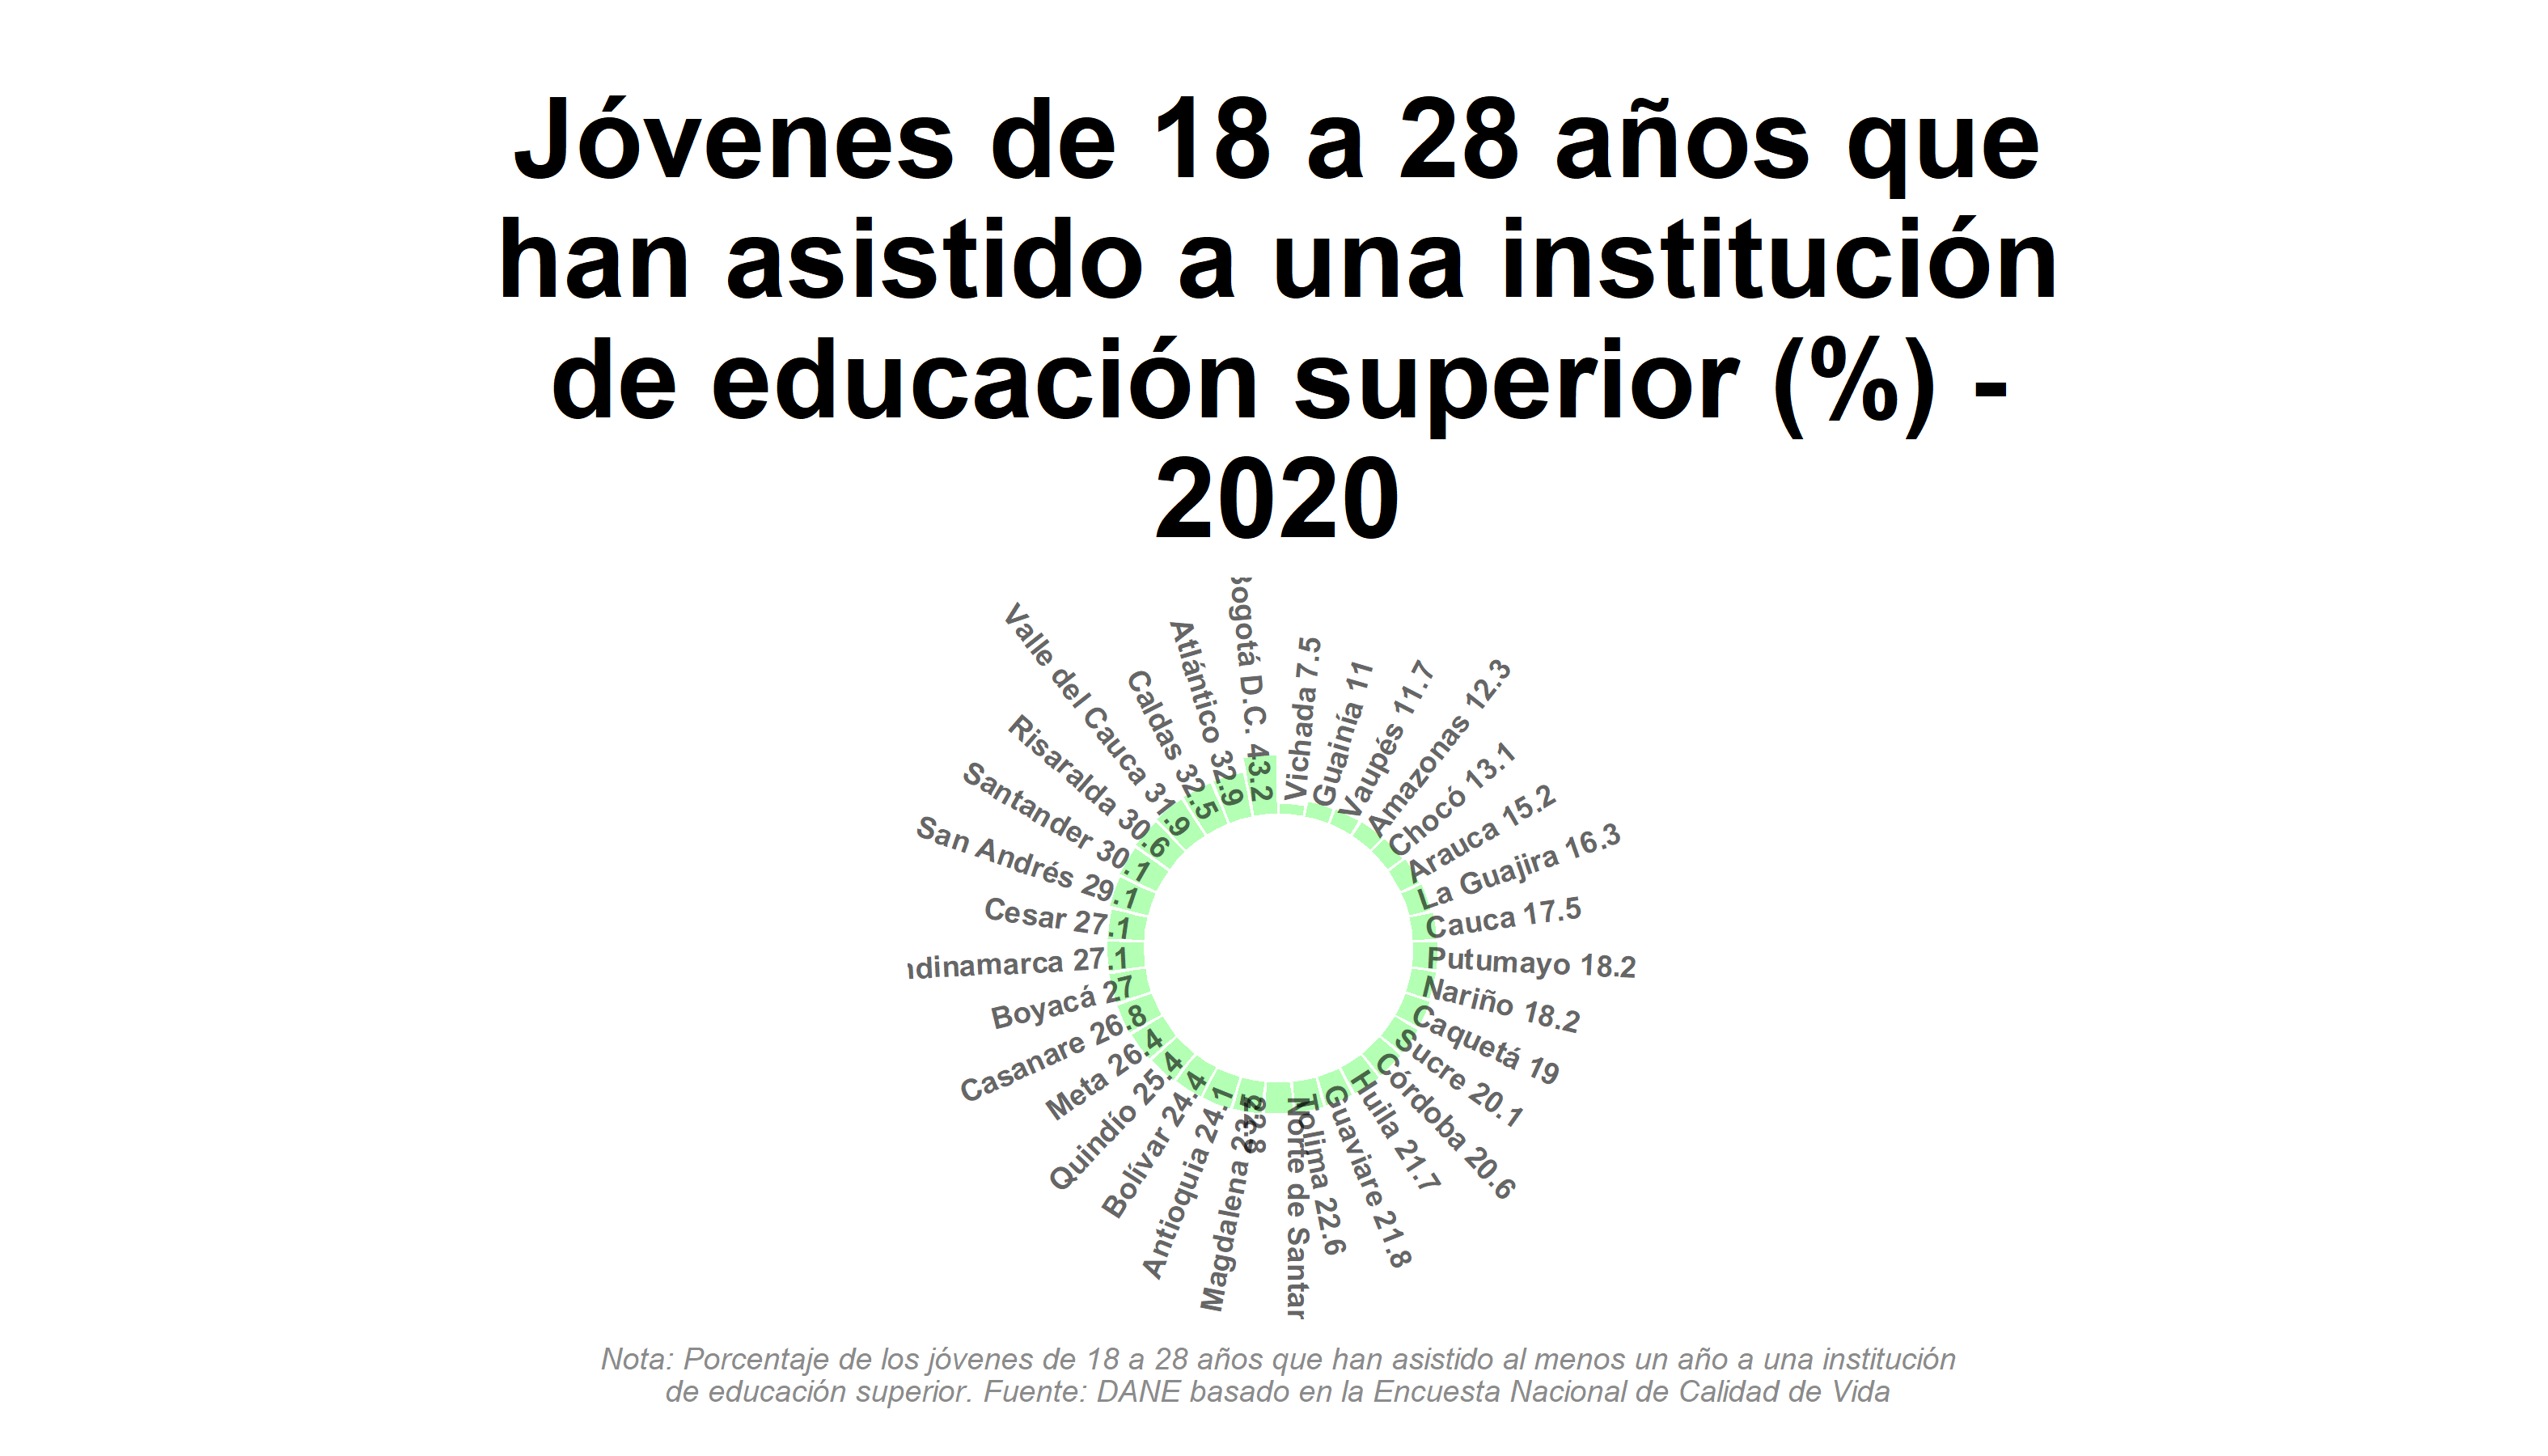
\includegraphics[width=\textwidth,keepaspectratio]{img/var_127_static.png}
        \end{center}
    \end{figure}
            \begin{itemize}
                \item Vichada es el territorio con menor porcentaje de jóvenes que han asistido a la educación superior con un 7.5\%, mientras que Bogotá es el de mayor asistencia con un 43.3\%, mostrando la desigualdad y heterogeneidad.
                \item Se resalta que la diferencia entre Bogotá y Atlántico, el segundo territorio con mayor asistencias, es de aproximadamente un 10\%.
                \item Se evidencia que los territorios en el centro del país tienen más jóvenes que asisten a una institución de educación superior, mientras que en la periferia, especialmente por el oriente y la Amazonia, se encuentran los territorios con menor asistencia para el 2020 (gráfica map 127 2020).
                \end{itemize}

%%%% Include figures
    \begin{figure}[H]
        \caption{Jóvenes de 18 a 28 años que han asistido a una institución de educación superior por zonas \label{map_result_2} }
        \begin{center}
        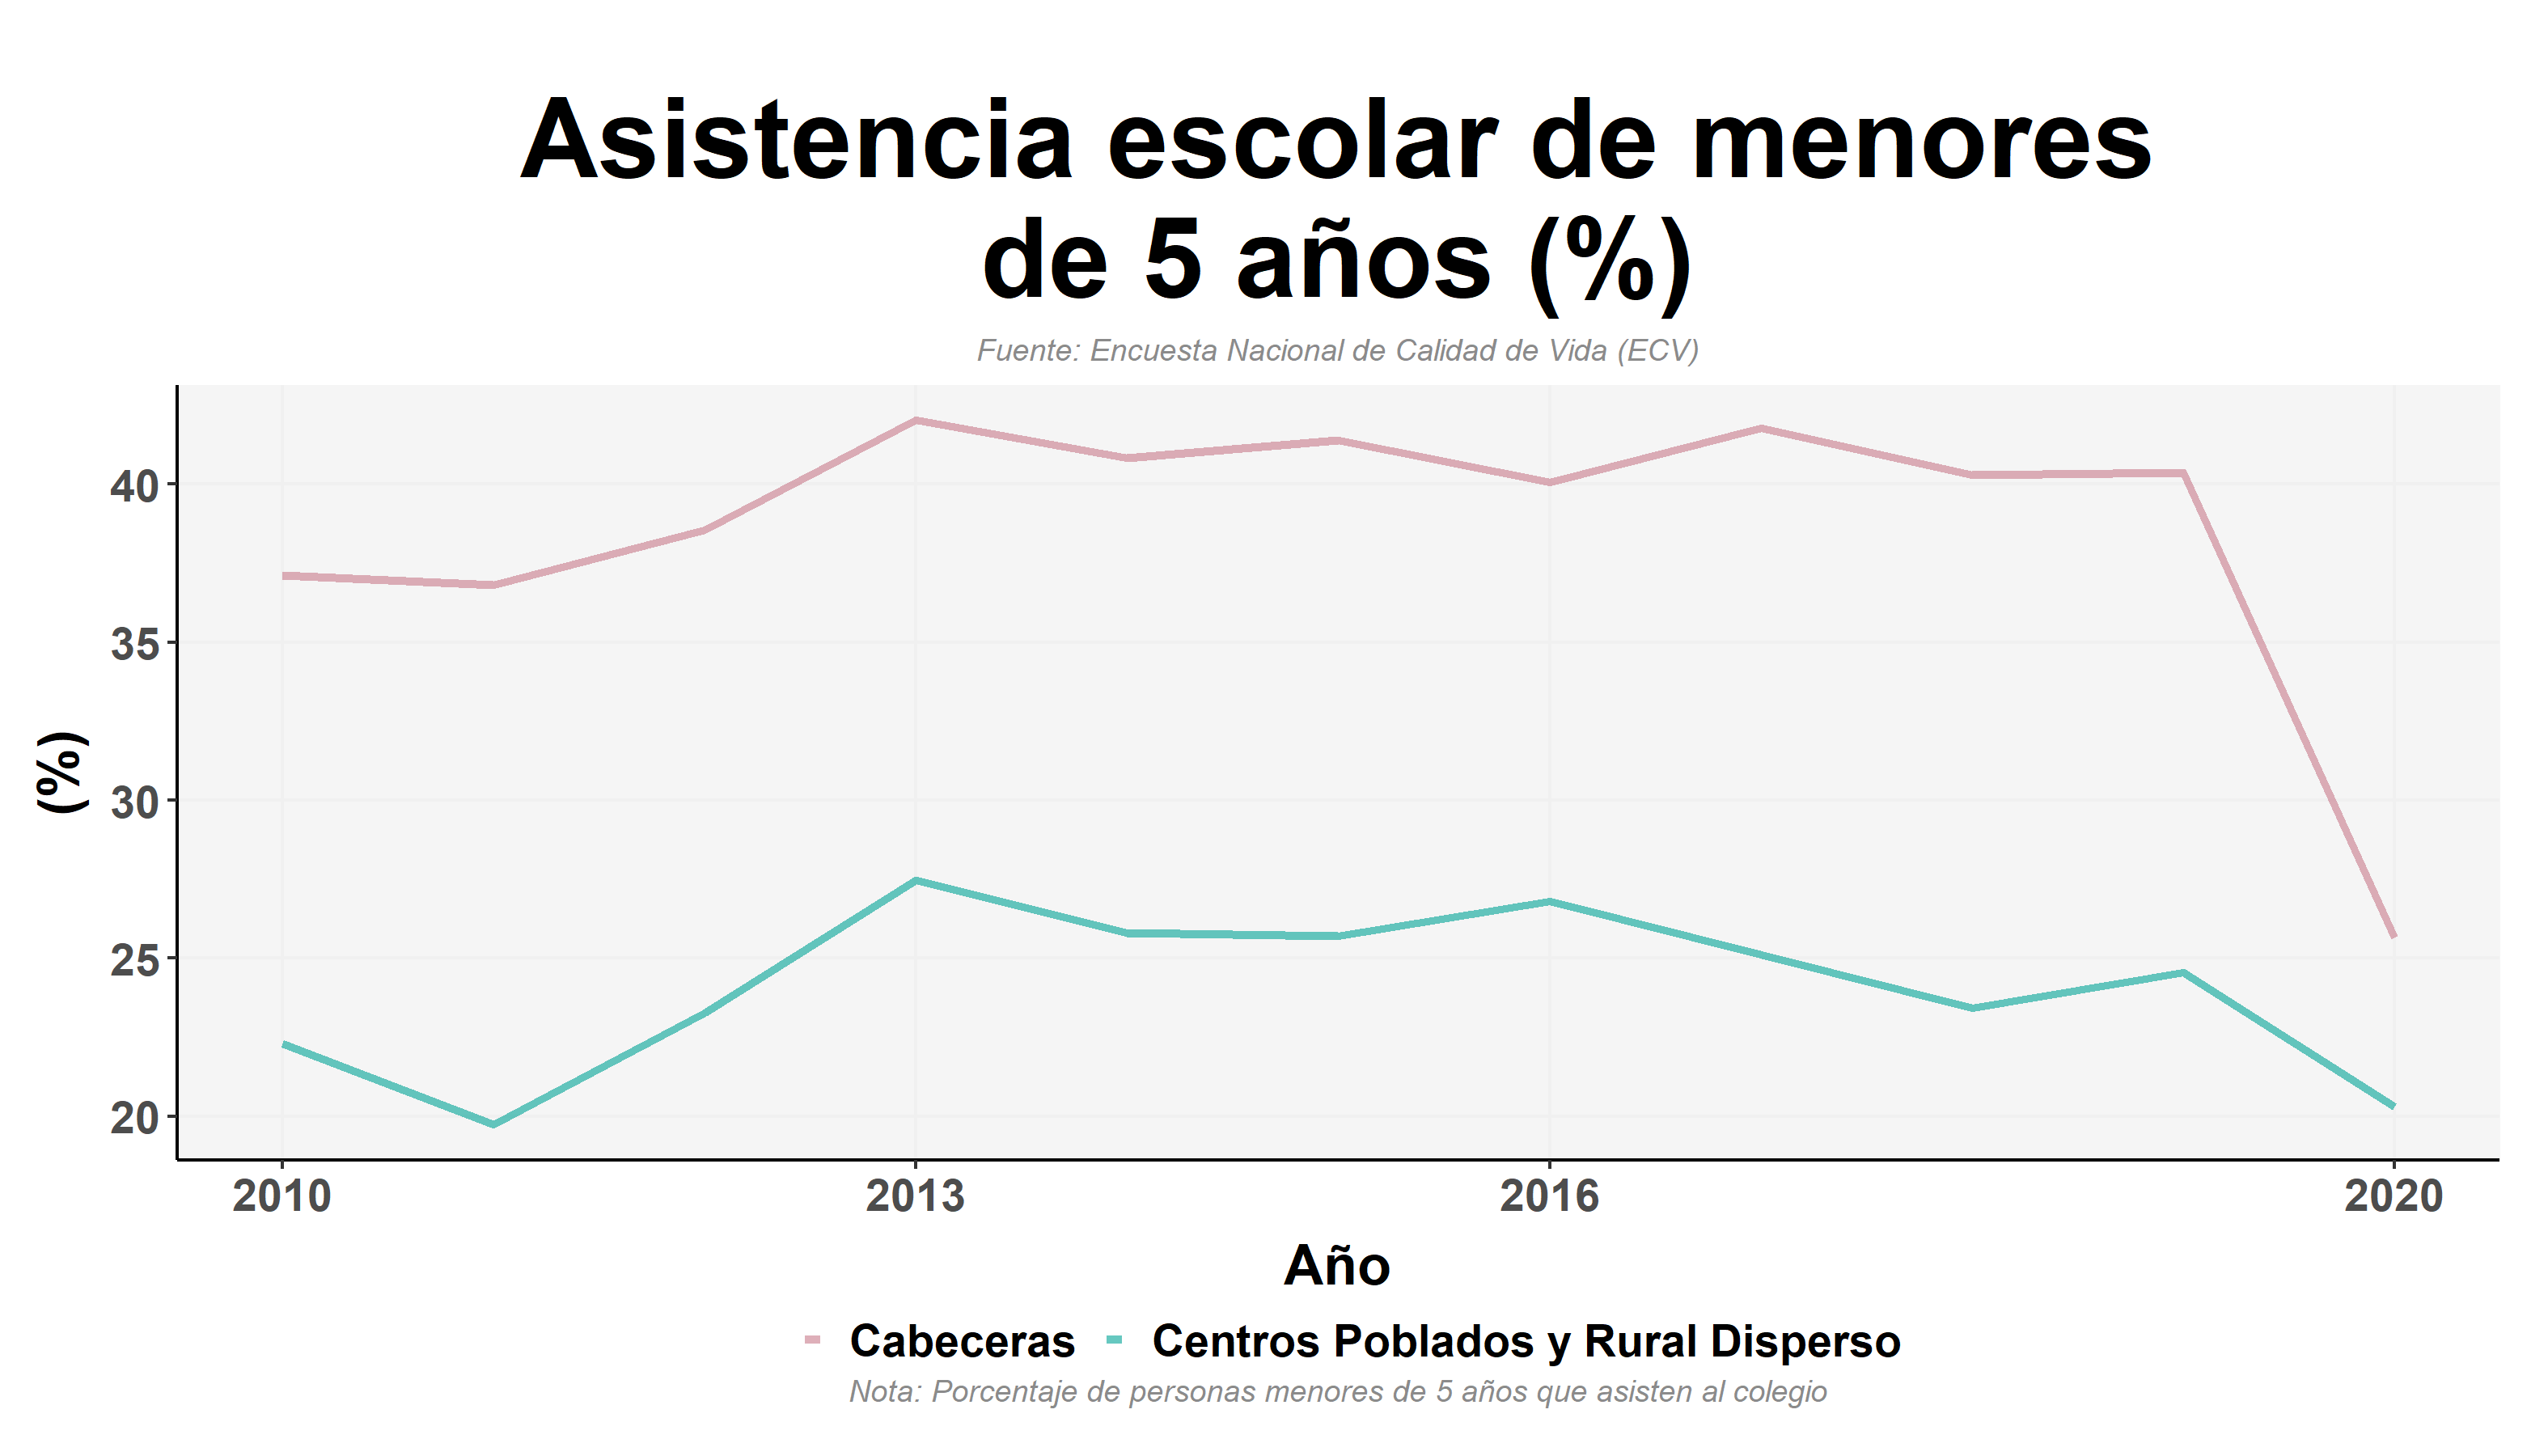
\includegraphics[width=\textwidth,keepaspectratio]{img/var_128_trend.png}
        \end{center}
    \end{figure}
            \begin{itemize}
                \item En la zona rural se ve un incremento constantes en los últimos 11 años, teniendo para 2020 un mayor porcentaje de jóvenes que han asistido a instituciones de educación superior a los registrados en 2010. Mientras que en la zona urbana se ve una leve disminución desde 2017.
                \item Encontramos que en las cabeceras el porcentaje de jóvenes es aproximadamente 3 veces los registrados en las zonas rurales.
                \item La brecha entre las zonas se ha mantenido a niveles similares a lo largo del tiempo.
                \end{itemize}

    \subsection{Calidad de la educación}
        \subsubsection{PENDIENTE - Tamaño de clase en secundaria y media}

%%%% Include figures
    \begin{figure}[H]
        \caption{Tamaño de clase en secundaria y media a nivel nacional \label{map_result_2} }
        \begin{center}
        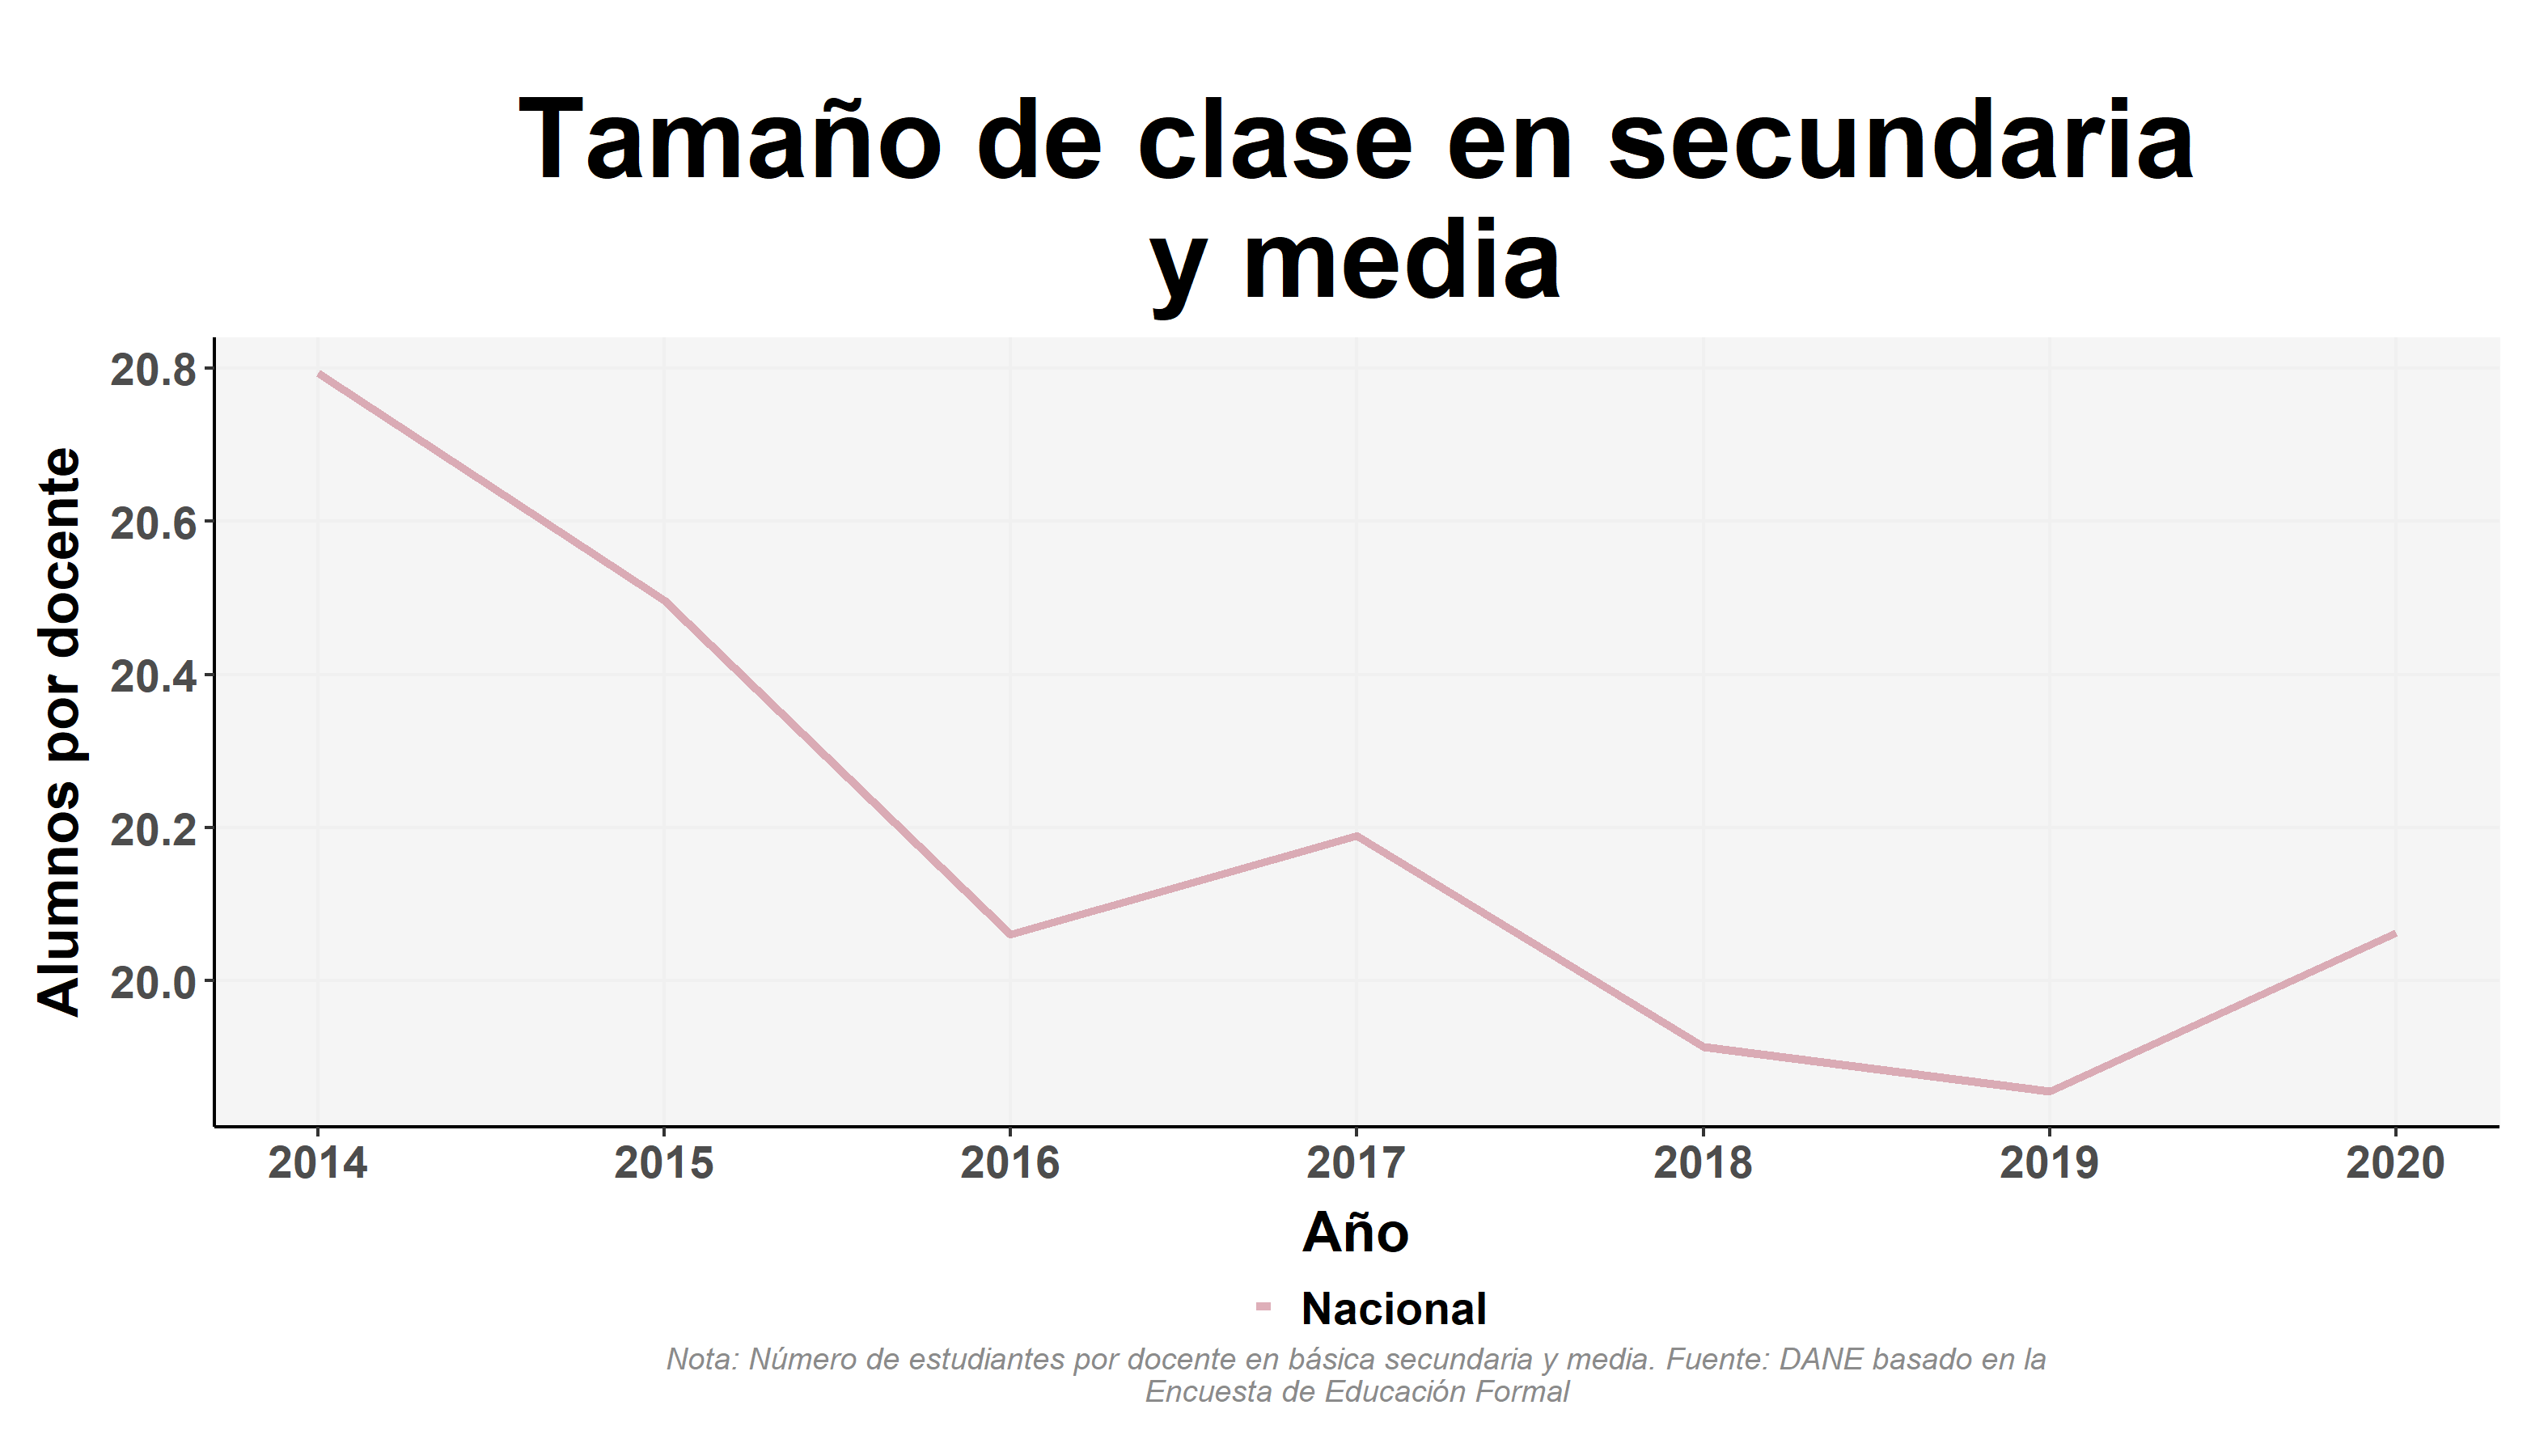
\includegraphics[width=\textwidth,keepaspectratio]{img/var_231_trend.png}
        \end{center}
    \end{figure}
            \begin{itemize}
                \item A nivel nacional el tamaño de la clase a disminuido a pesar del pico que presentó en 2017 y 2020.
                \item El aumento del tamaño de la clase para 2020 llevó a un retroceso a los niveles registrados en 2016, aunque aún continua con una mejora comparado a los del 2014.
                \end{itemize}

    \subsection{Fecundidad adolescente}

%%%% Include figures
    \begin{figure}[H]
        \caption{Tasa de fecundidad en mujeres jóvenes por departamentos - 2010 VS 2019 \label{map_result_2} }
        \begin{center}
        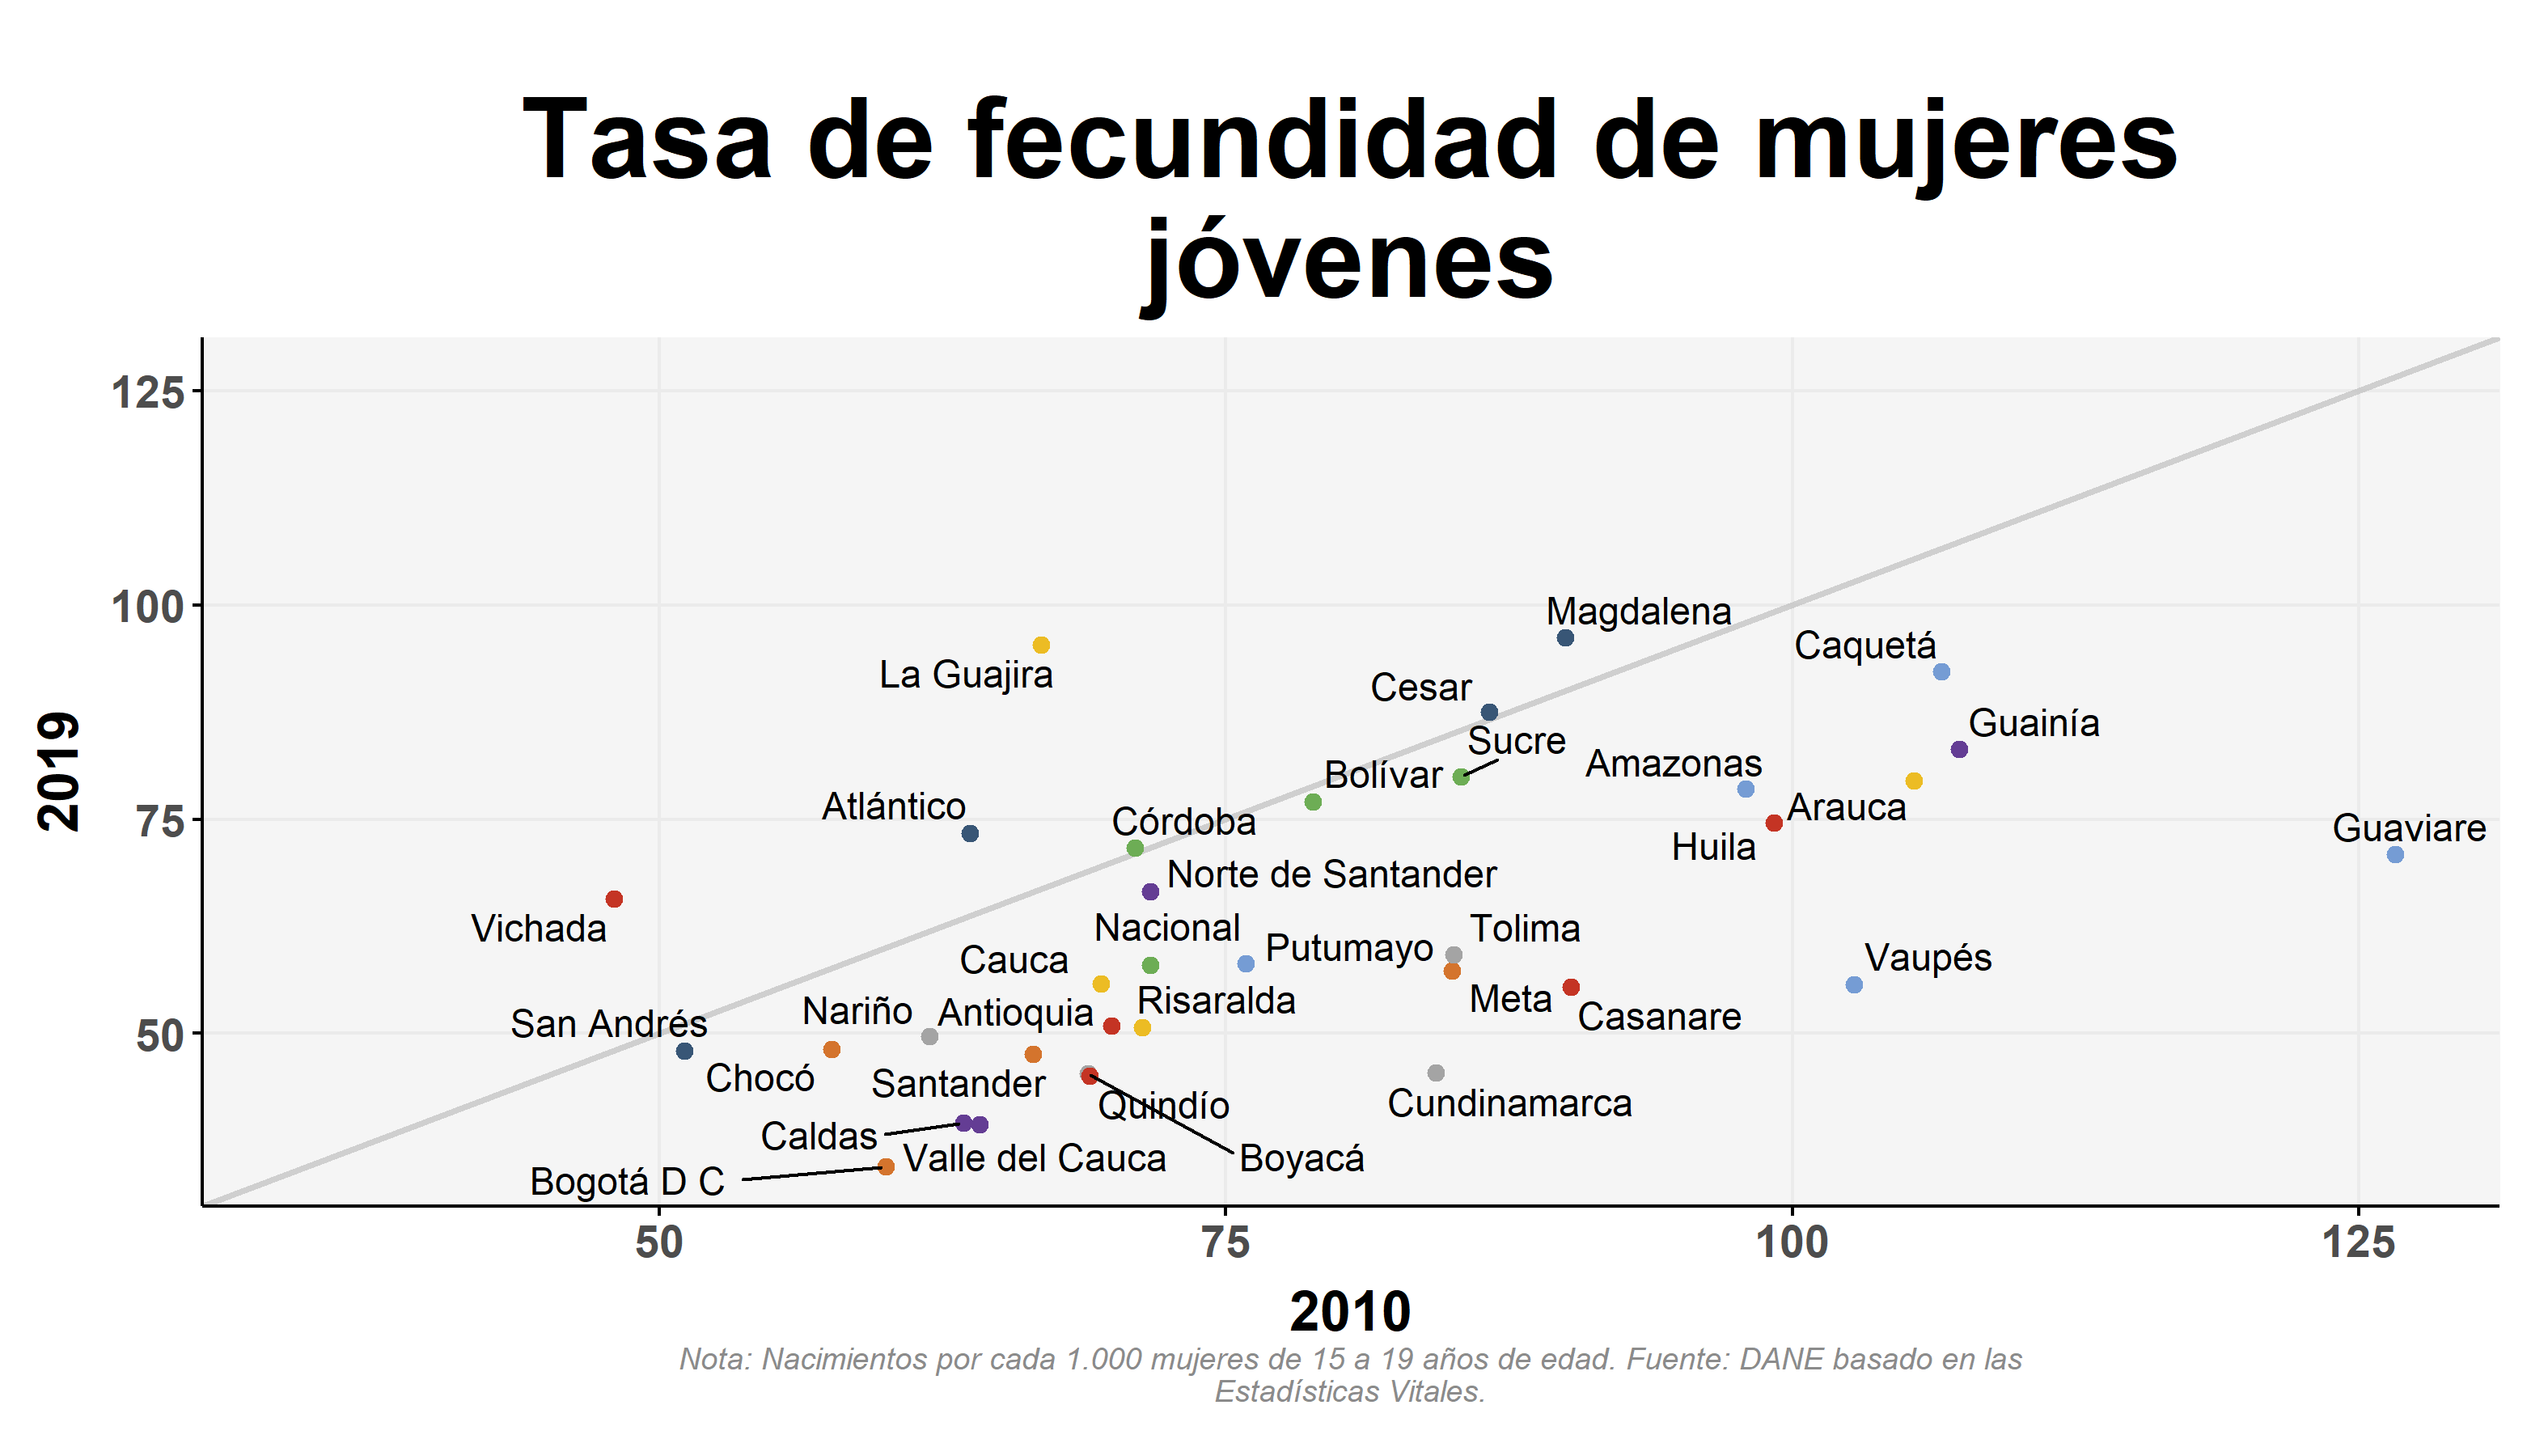
\includegraphics[width=\textwidth,keepaspectratio]{img/var_282_scatter_time.png}
        \end{center}
    \end{figure}
            \begin{itemize}
                \item En general la tasa de fecundidad en mujeres entre 15 a 19 años ha disminuido en la mayoría de los territorios.
                \item La Guajira, Vichada, Atlántico y Magdalena son los territorios donde aumentó la tasa de manera significativa, en especial el primero que pasó de estar en el promedio nacional en el promedio nacional en 2010 y pasó a ser la segunda tasa más alta en 2019.
                \item Guaviare, Vaupés, Cundinamarca y Casanare obtuvieron la mayor disminución, en especial Guaviare que pasó de tener la tasa más alta, por encima de 125 nacimientos por cada mil mujeres para 2010, a una de alrededor de 75 para 2019.
                \end{itemize}

%%%% Include figures
    \begin{figure}[H]
        \caption{Tasa de fecundidad en mujeres jóvenes por departamentos para 2019 \label{map_result_2} }
        \begin{center}
        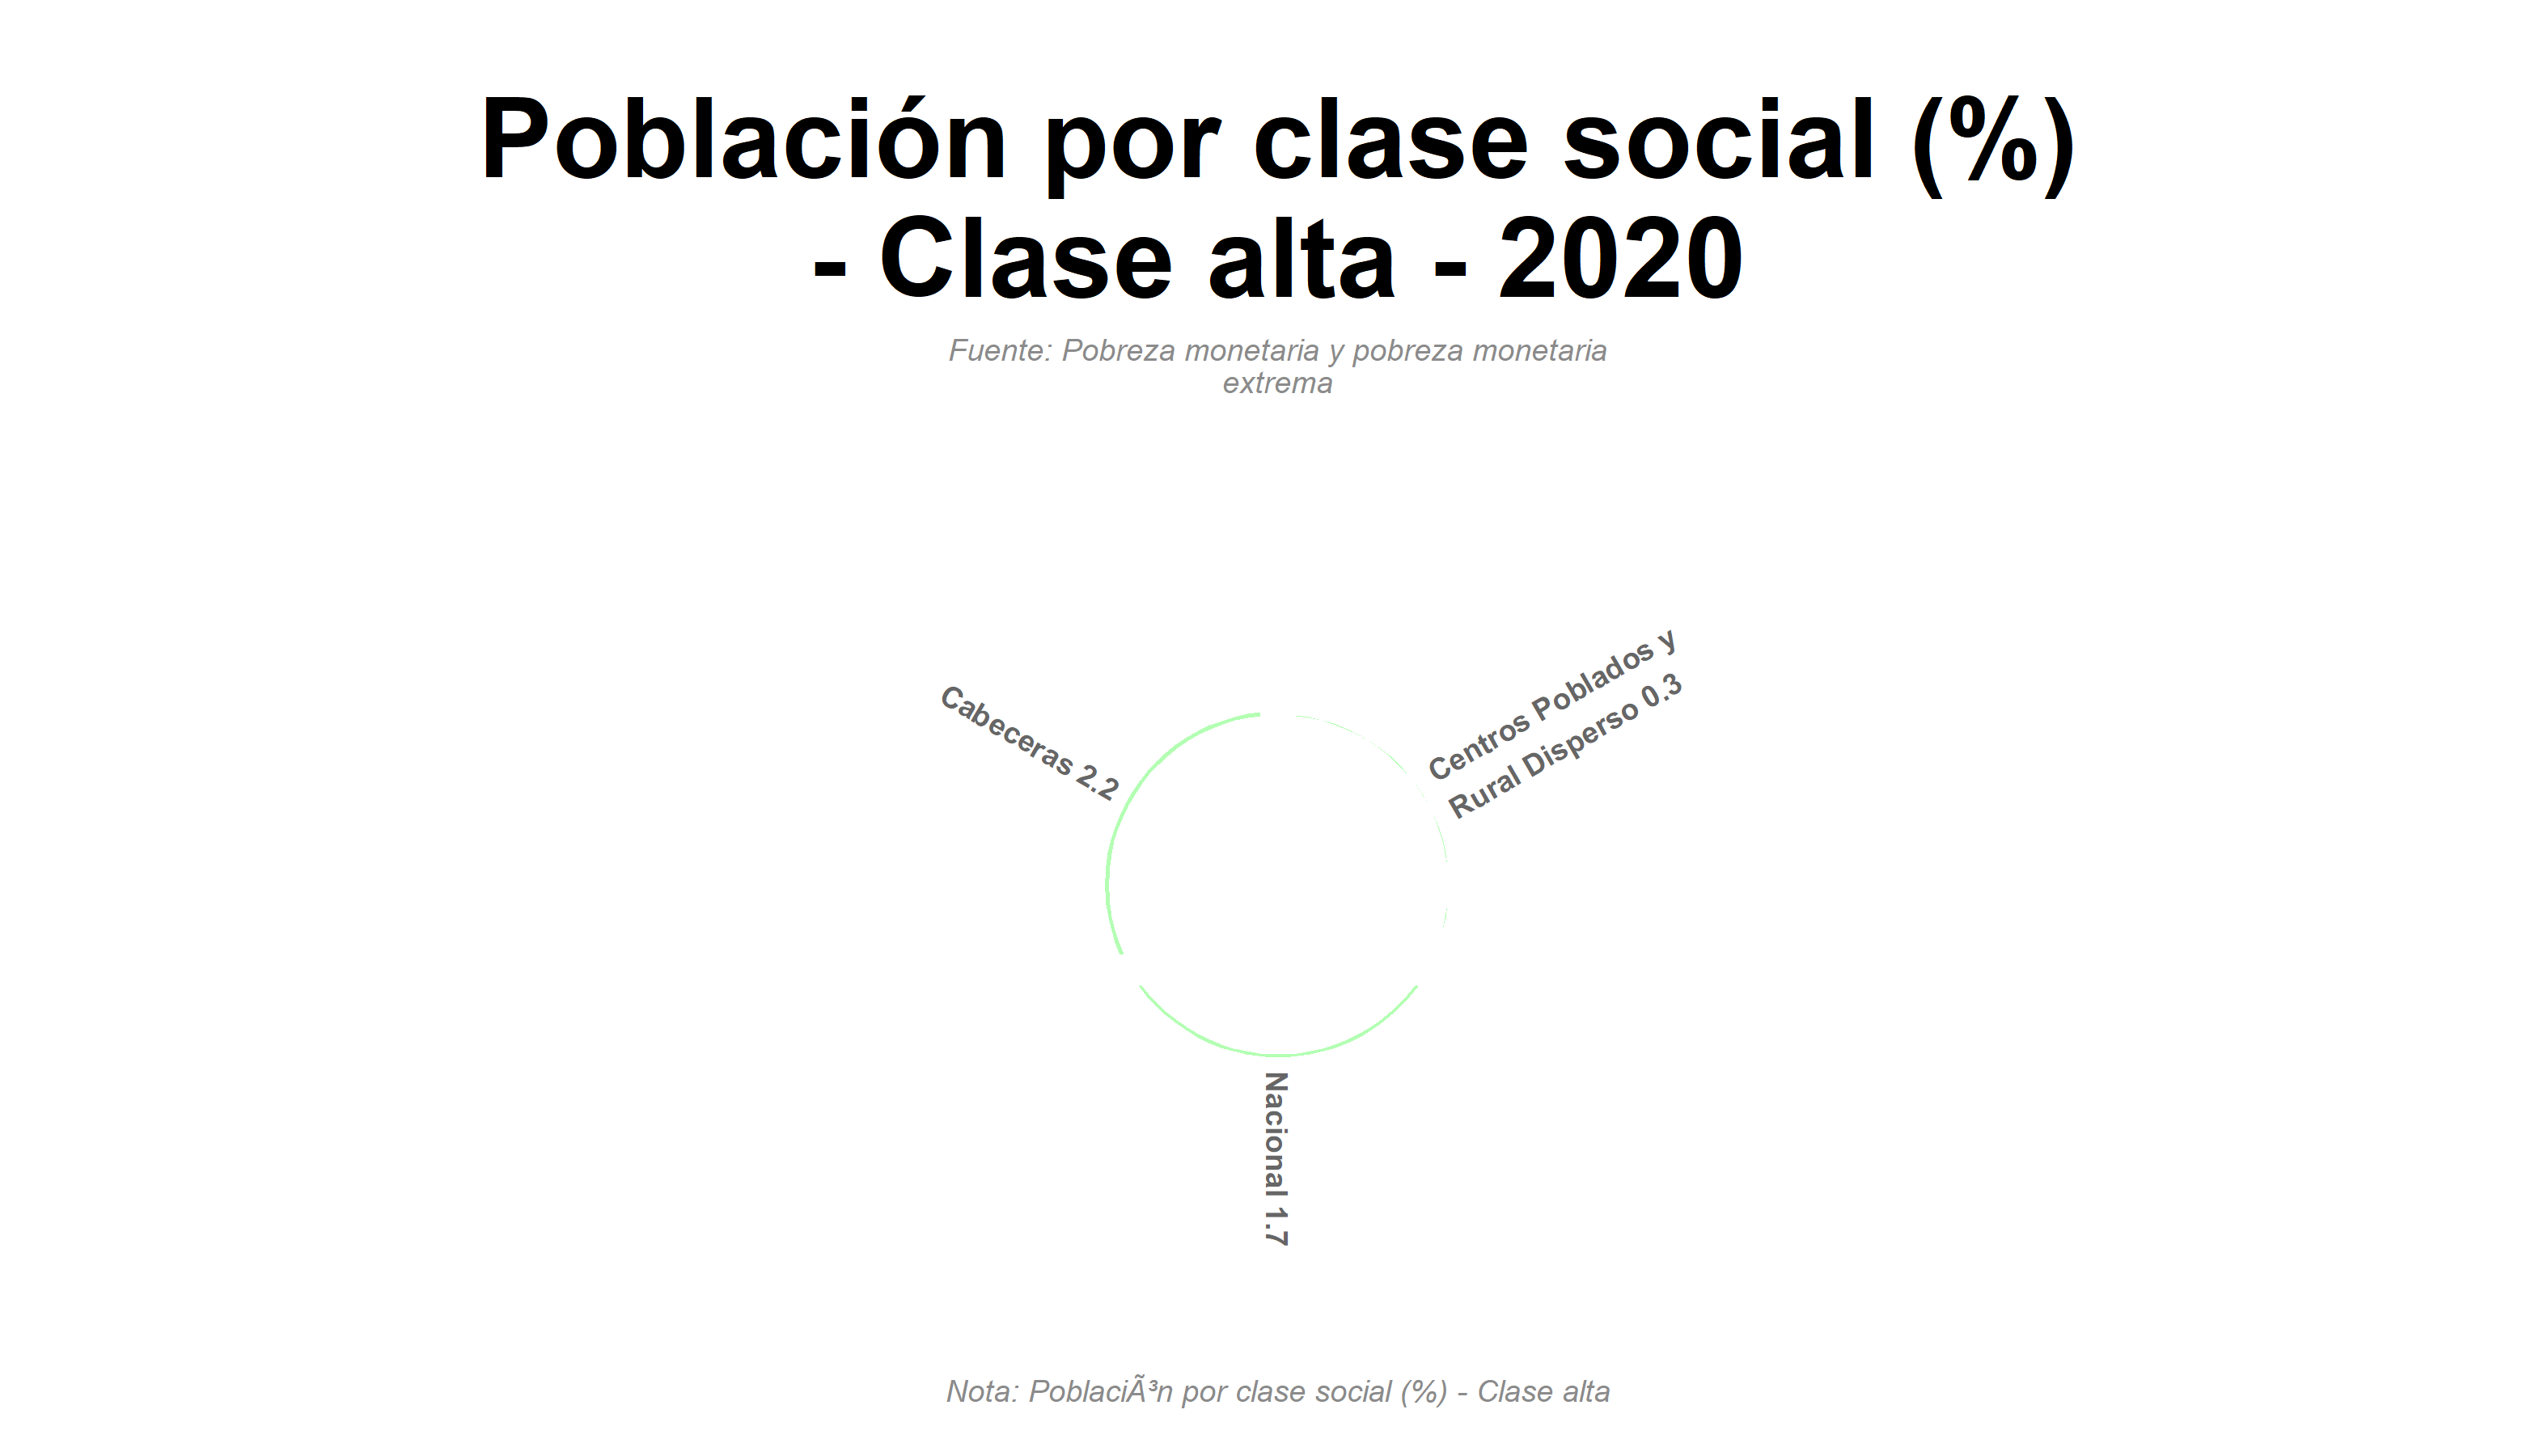
\includegraphics[width=\textwidth,keepaspectratio]{img/var_282_static.png}
        \end{center}
    \end{figure}
            \begin{itemize}
                \item La tasa de fecundidad adolescente en Bogotá es de 34.4 nacimientos por cada mil mujeres, siendo la más baja, mientras que el Magdalena tiene la tasa más alta con 96.2 nacimientos, mostrando la desigualdad.
                \item Los territorios con la tasa de fecundidad más alta se concentran en la región Caribe, mientras que los de menor tasa están en la zona central y occidental del país.
                \end{itemize}

%%%% Include figures
    \begin{figure}[H]
        \caption{Tasa de fecundidad en mujeres jóvenes a nivel nacional \label{map_result_2} }
        \begin{center}
        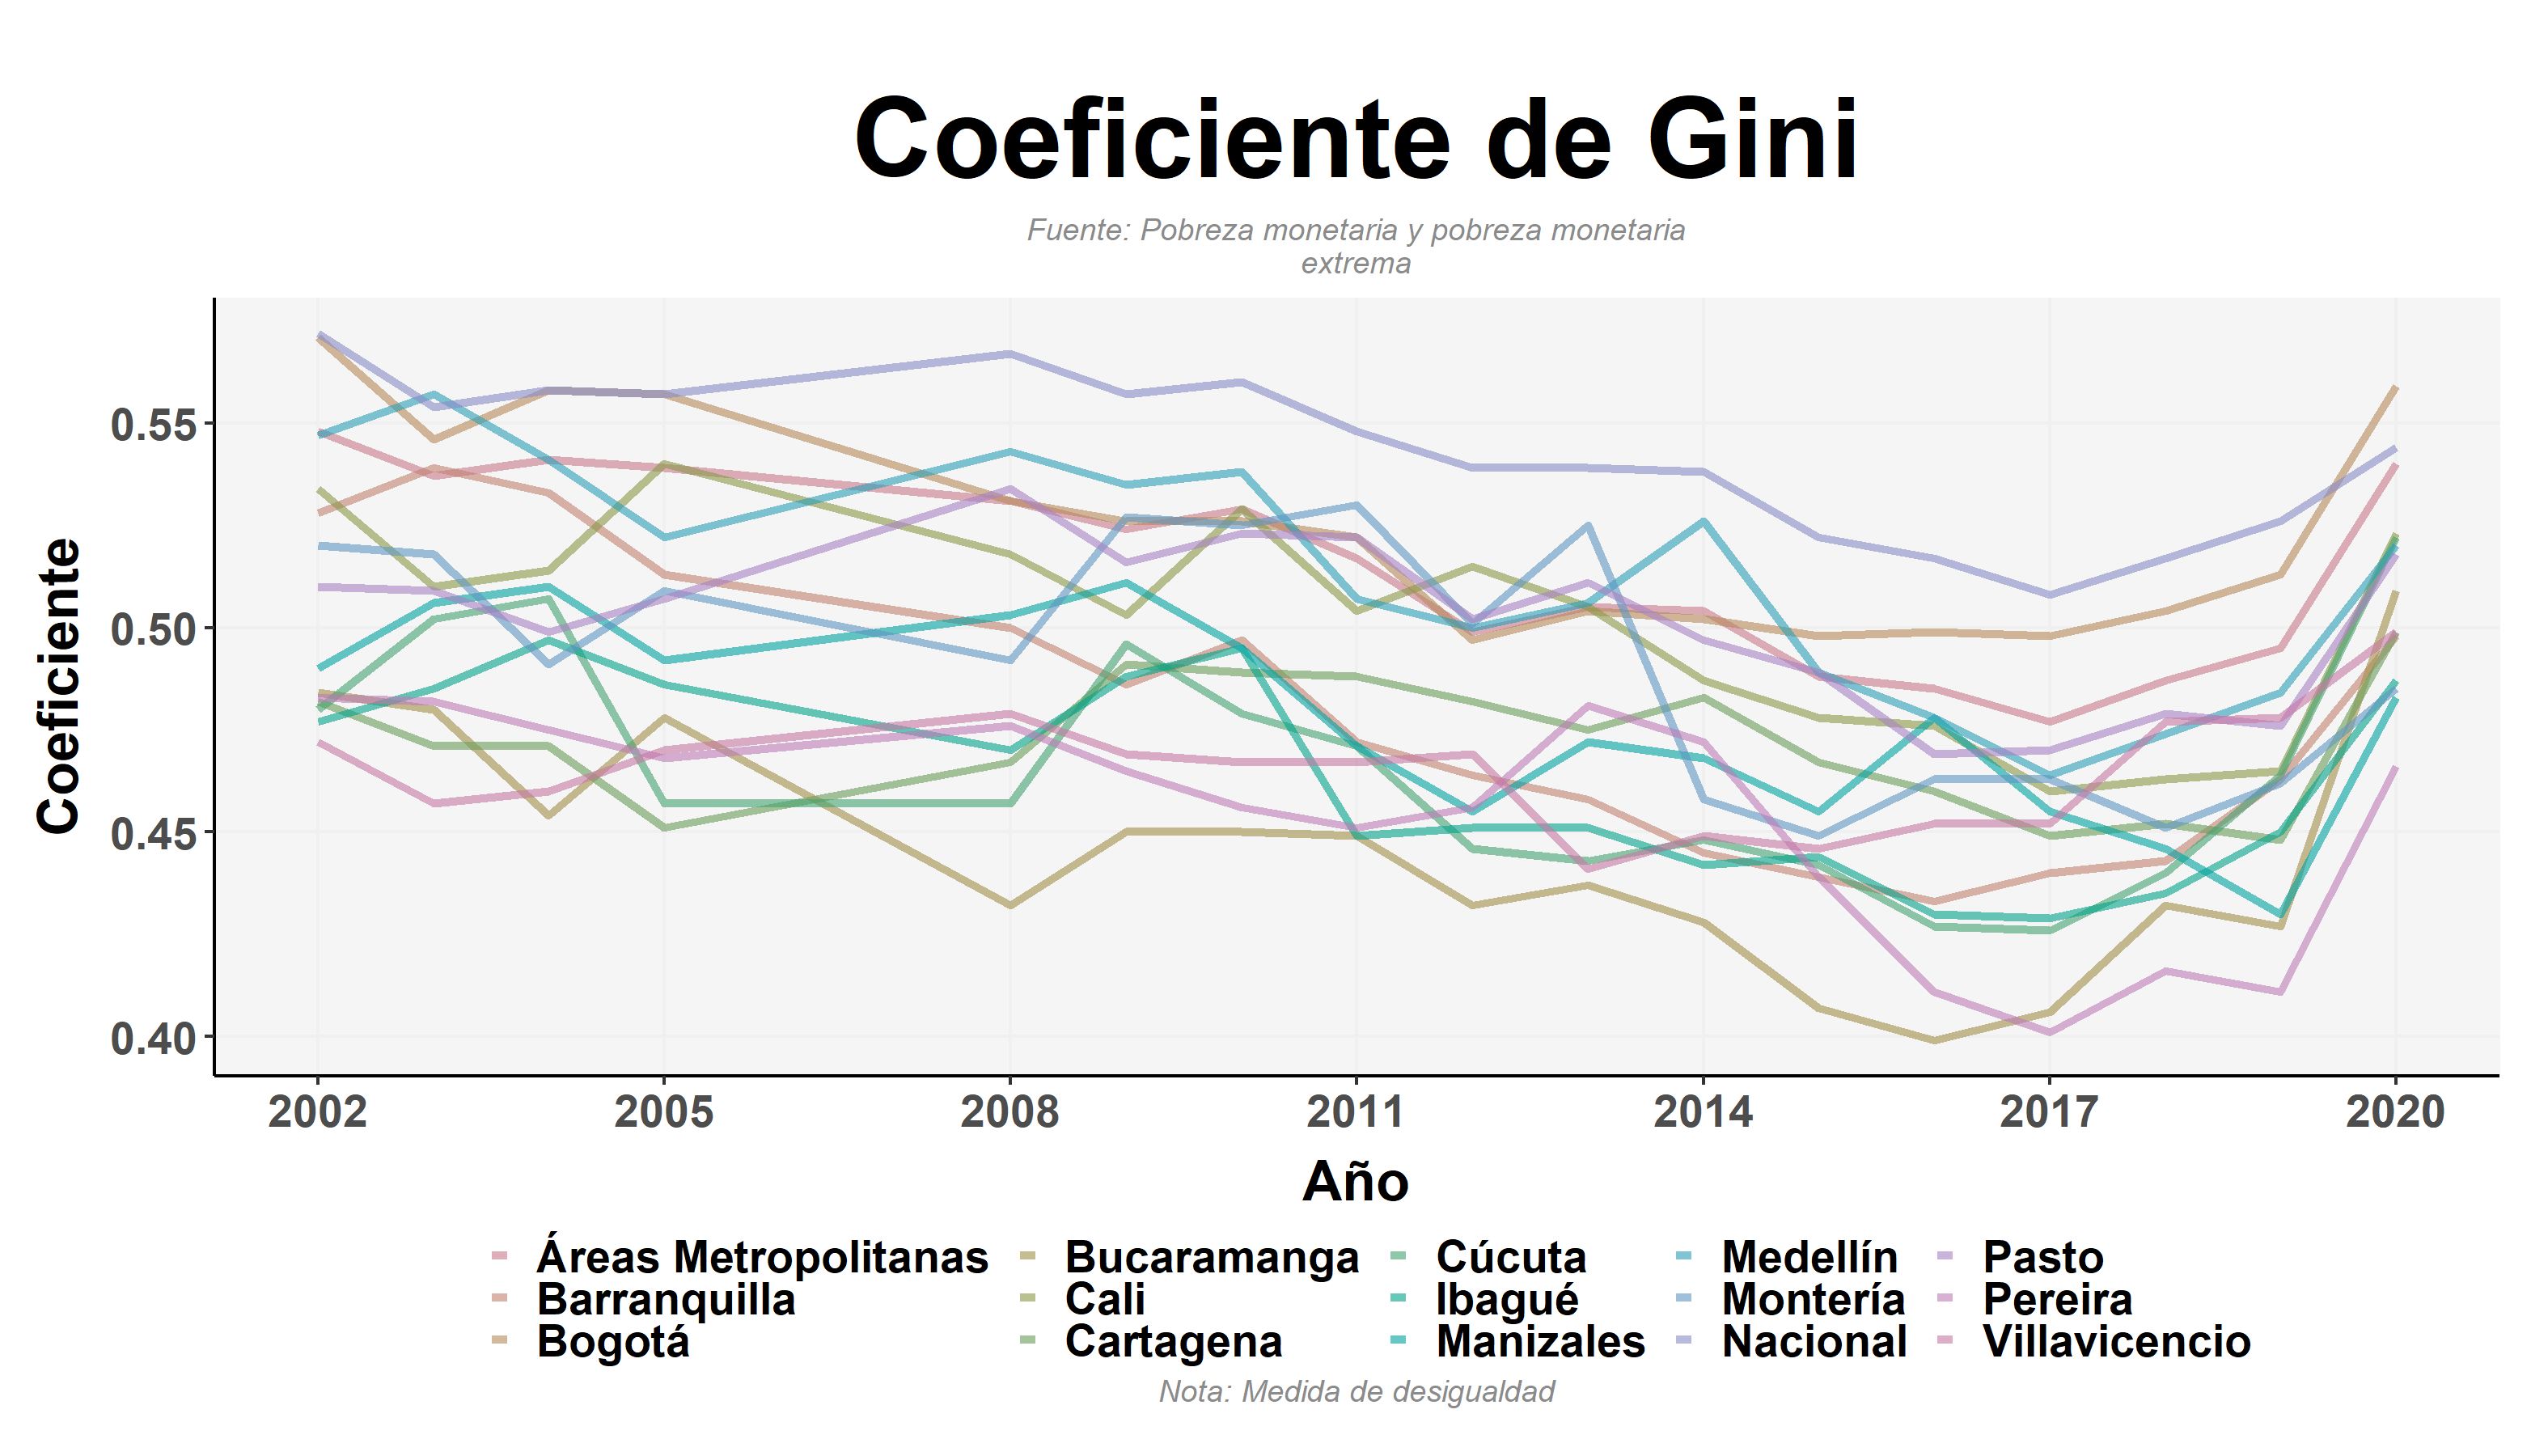
\includegraphics[width=\textwidth,keepaspectratio]{img/var_283_trend.png}
        \end{center}
    \end{figure}
            \begin{itemize}
                \item A nivel nacional se ha venido disminuyendo constantemente desde el 2012, pasando de tener valores por encima de 70 nacimientos por cada mil mujeres de 15 a 19 años, a estar por debajo de los 60 nacimientos.
                \end{itemize}

    \subsection{Desempleo e inactividad}
        \subsubsection{Jóvenes que no estudian ni trabajan}

%%%% Include figures
    \begin{figure}[H]
        \caption{Porcentaje de jóvenes que no estudian, ni trabajan a nivel nacional \label{map_result_2} }
        \begin{center}
        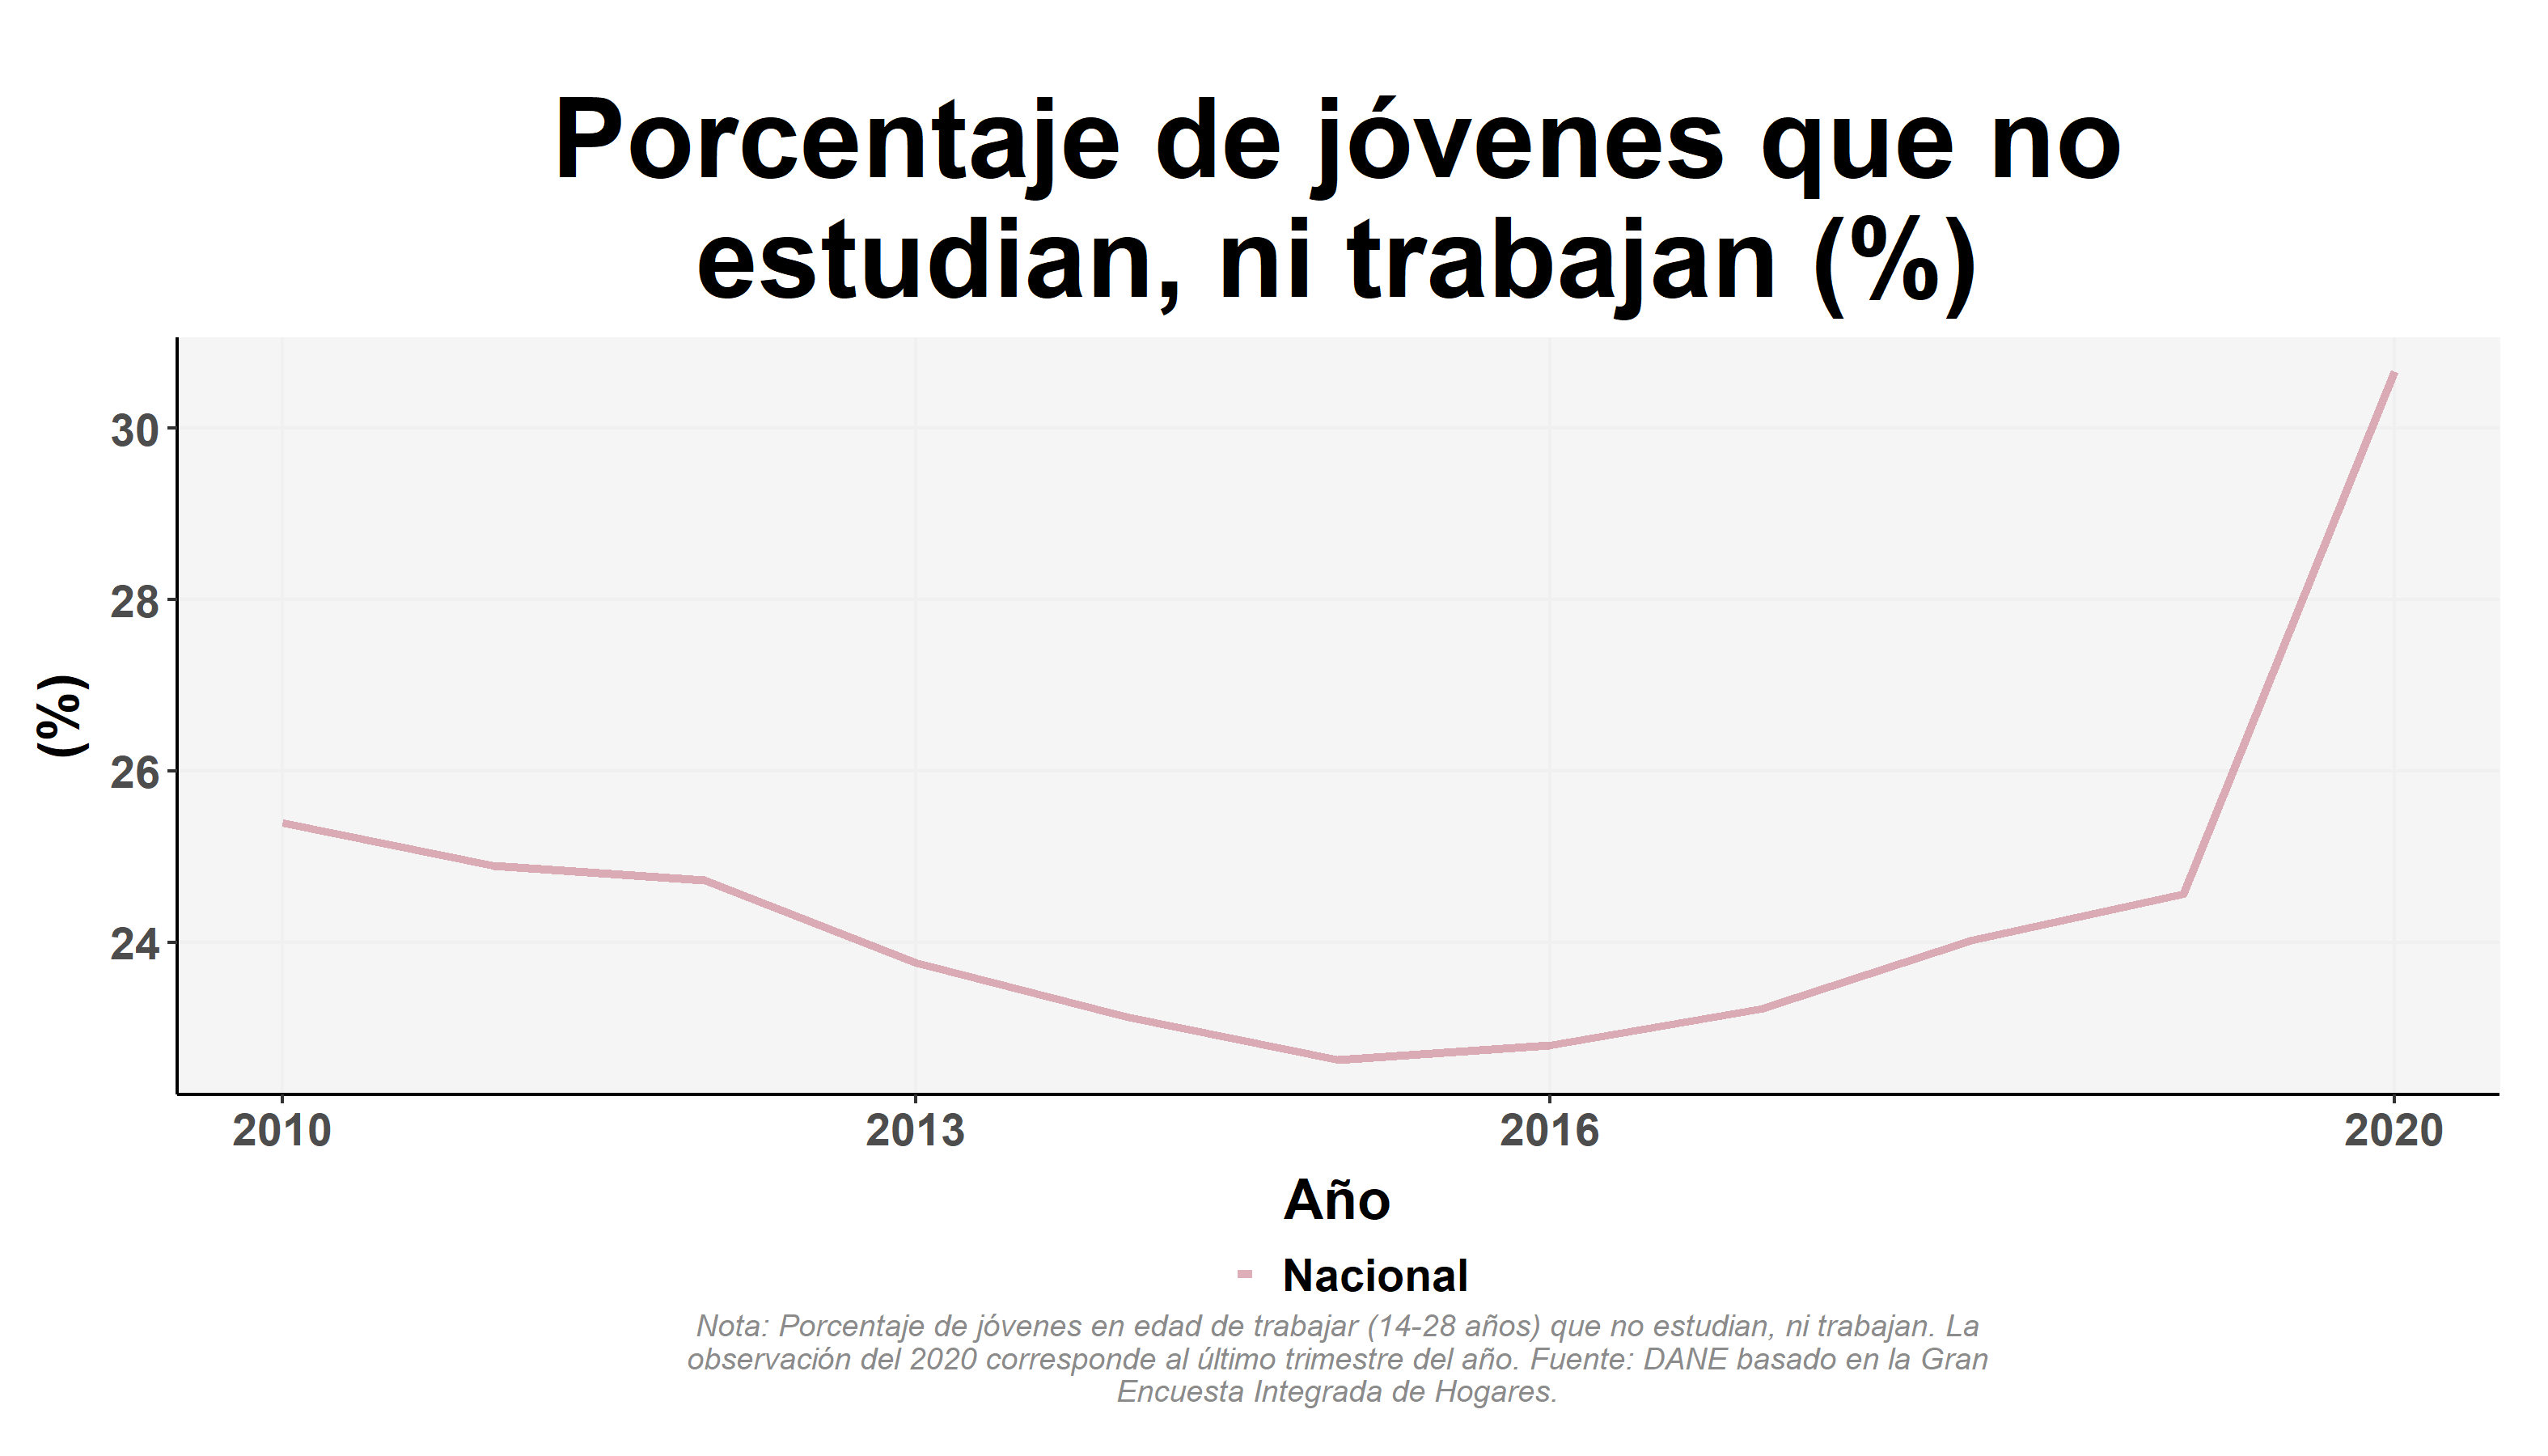
\includegraphics[width=\textwidth,keepaspectratio]{img/var_42_trend.png}
        \end{center}
    \end{figure}
            \begin{itemize}
                \item El porcentaje de jóvenes que no estudian ni trabajan estuvo disminuyendo en la primera mitad de la década pero a partir de 2016 volvió a incrementar.
                \item Aunque desde el 2016 estaba aumentando los ninis, en 2020 se evidencio un aumento pasando de ser alrededor del 25\% en 2019 a estar por encima del 30\% en 2020, estando por niveles superiores a los registrados en el 2010.
                \end{itemize}

%%%% Include figures
    \begin{figure}[H]
        \caption{Porcentaje de jóvenes que no estudian, ni trabajan por género \label{map_result_2} }
        \begin{center}
        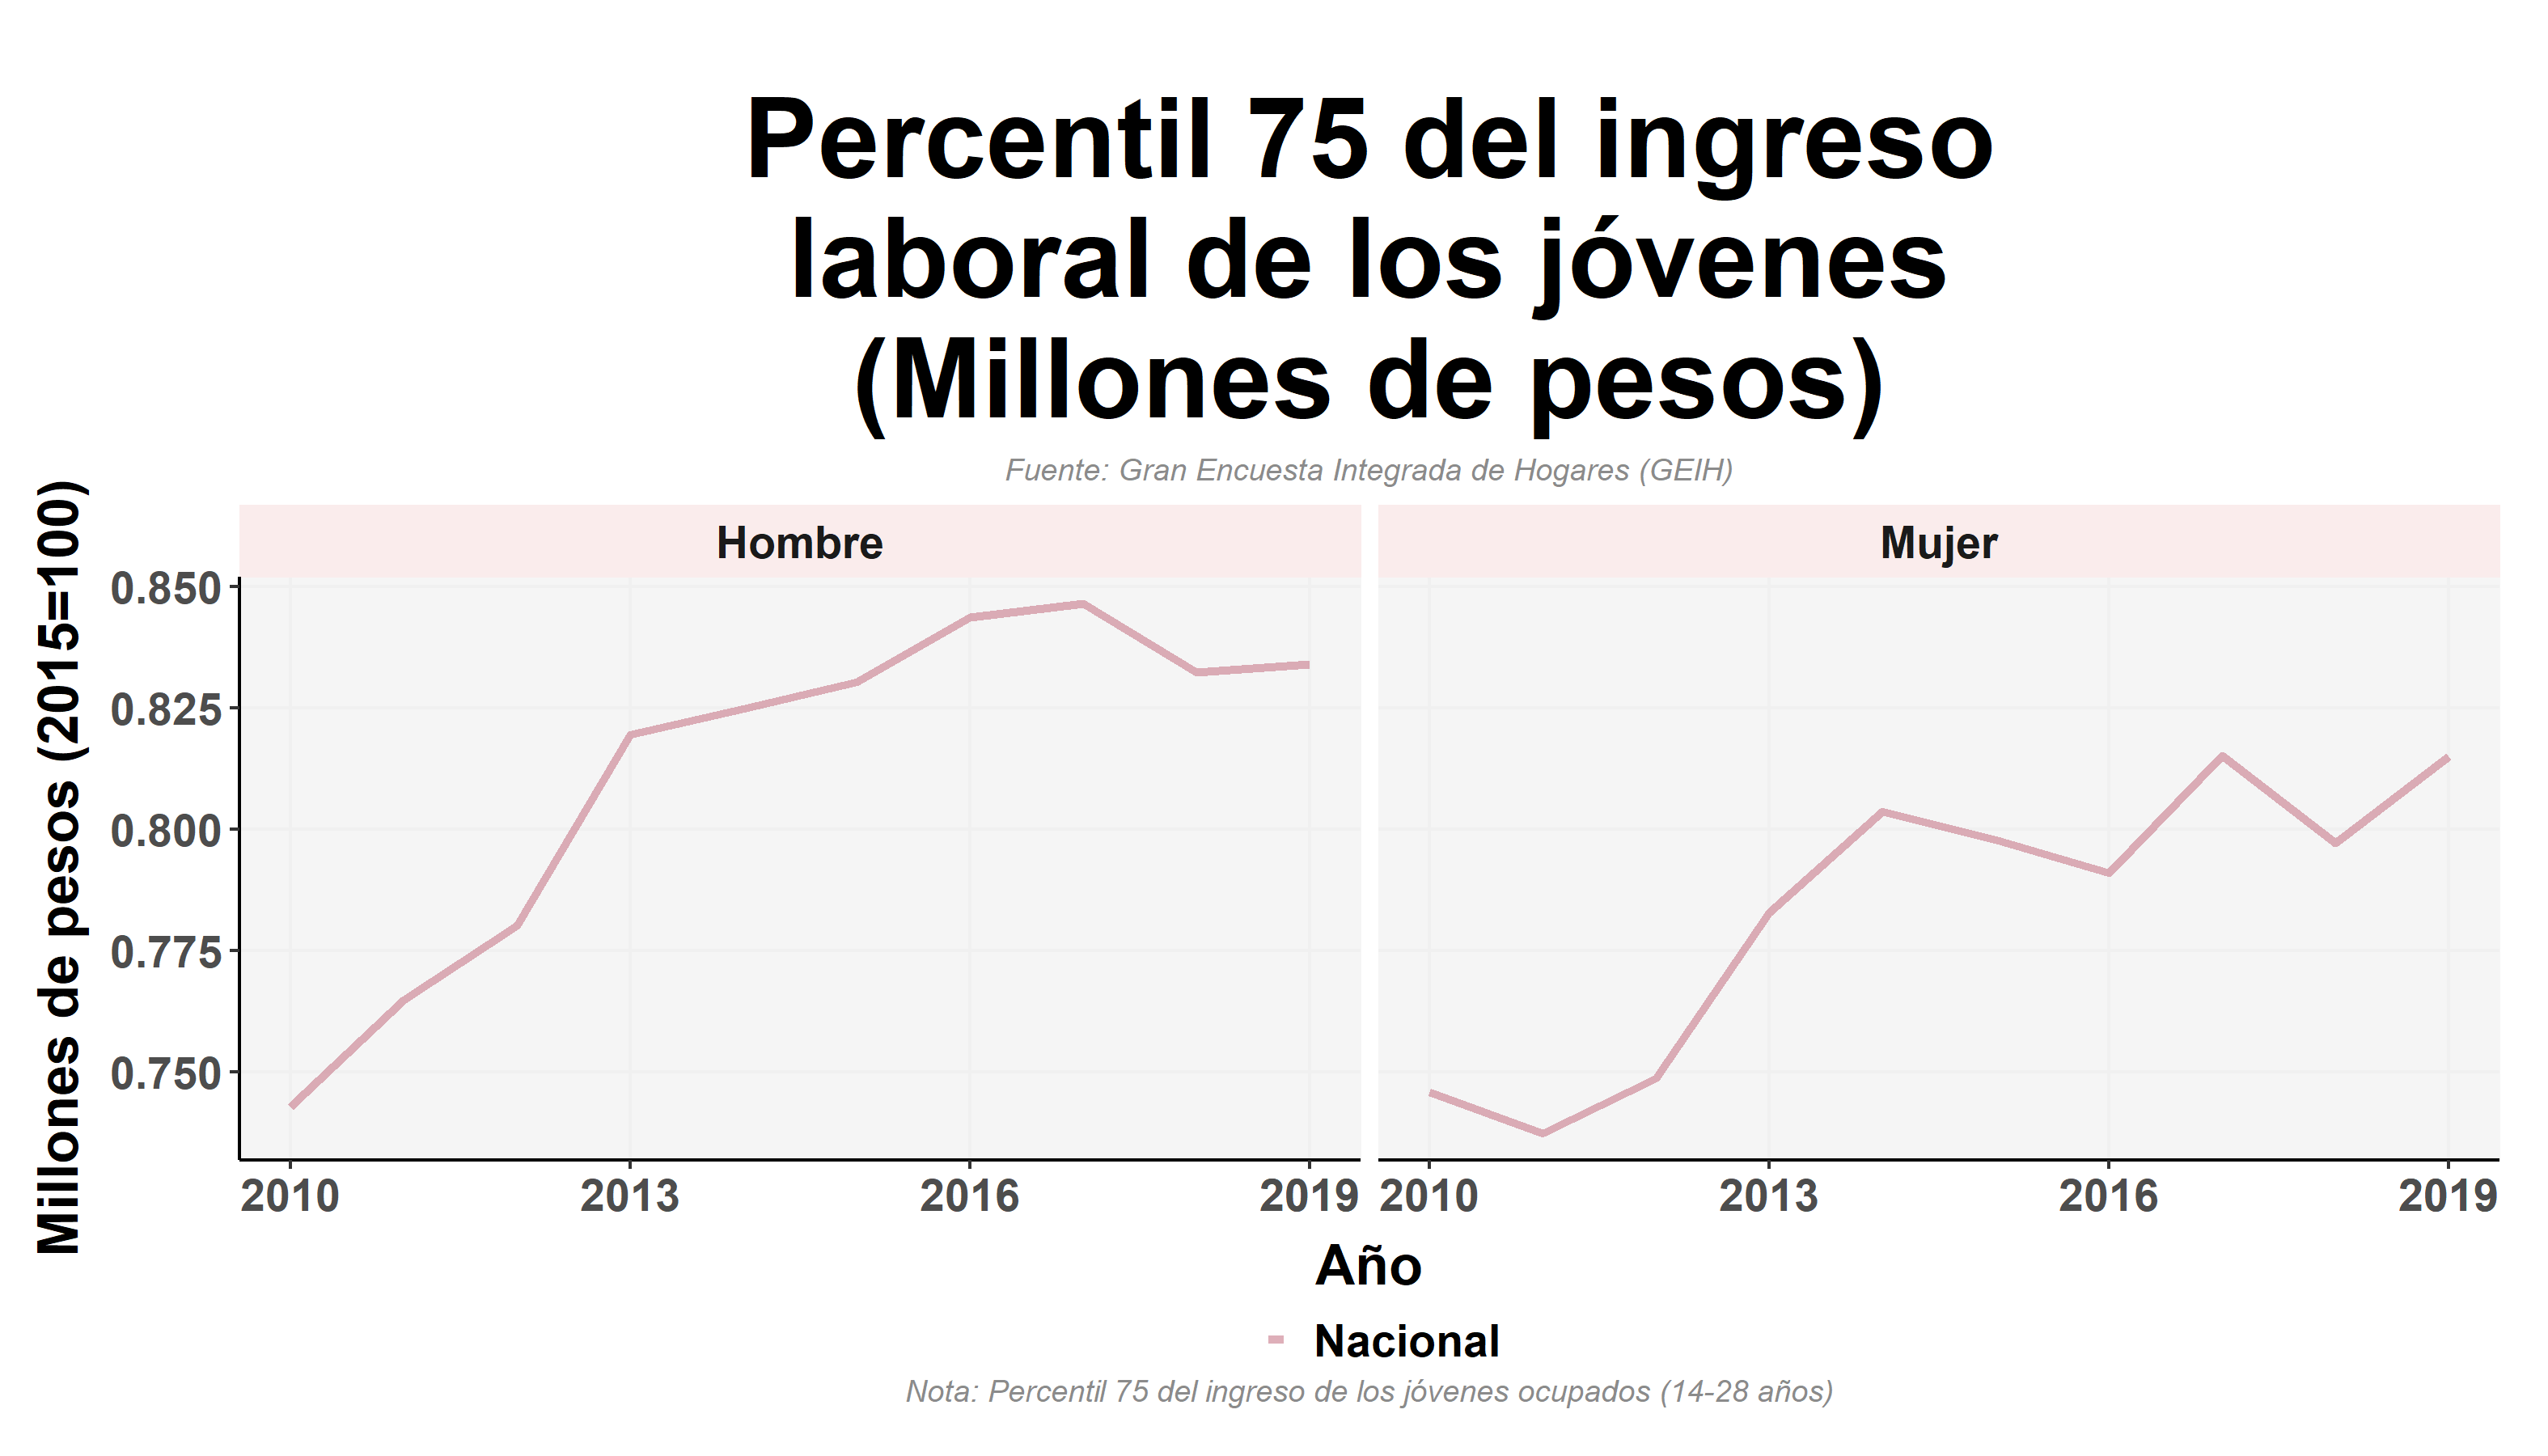
\includegraphics[width=\textwidth,keepaspectratio]{img/var_41_trend.png}
        \end{center}
    \end{figure}
            \begin{itemize}
                \item Hay una diferencia evidente entre los géneros, las mujeres jóvenes tienen el mayor porcentaje, siendo el doble que en los hombres.
                \item En ambos géneros la tendencia en los años tuvo el mismo comportamiento pero las variaciones son mayores en las mujeres.
                \item Para 2020 vemos que se presenta un aumento fuerte en ambos géneros, más pronunciado en las mujeres, que hace que lleguen a niveles mayores a los registrados hace 11 años.
                \end{itemize}

%%%% Include figures
    \begin{figure}[H]
        \caption{Porcentaje de jóvenes que no estudian, ni trabajan por minorías y no minorías para 2020 \label{map_result_2} }
        \begin{center}
        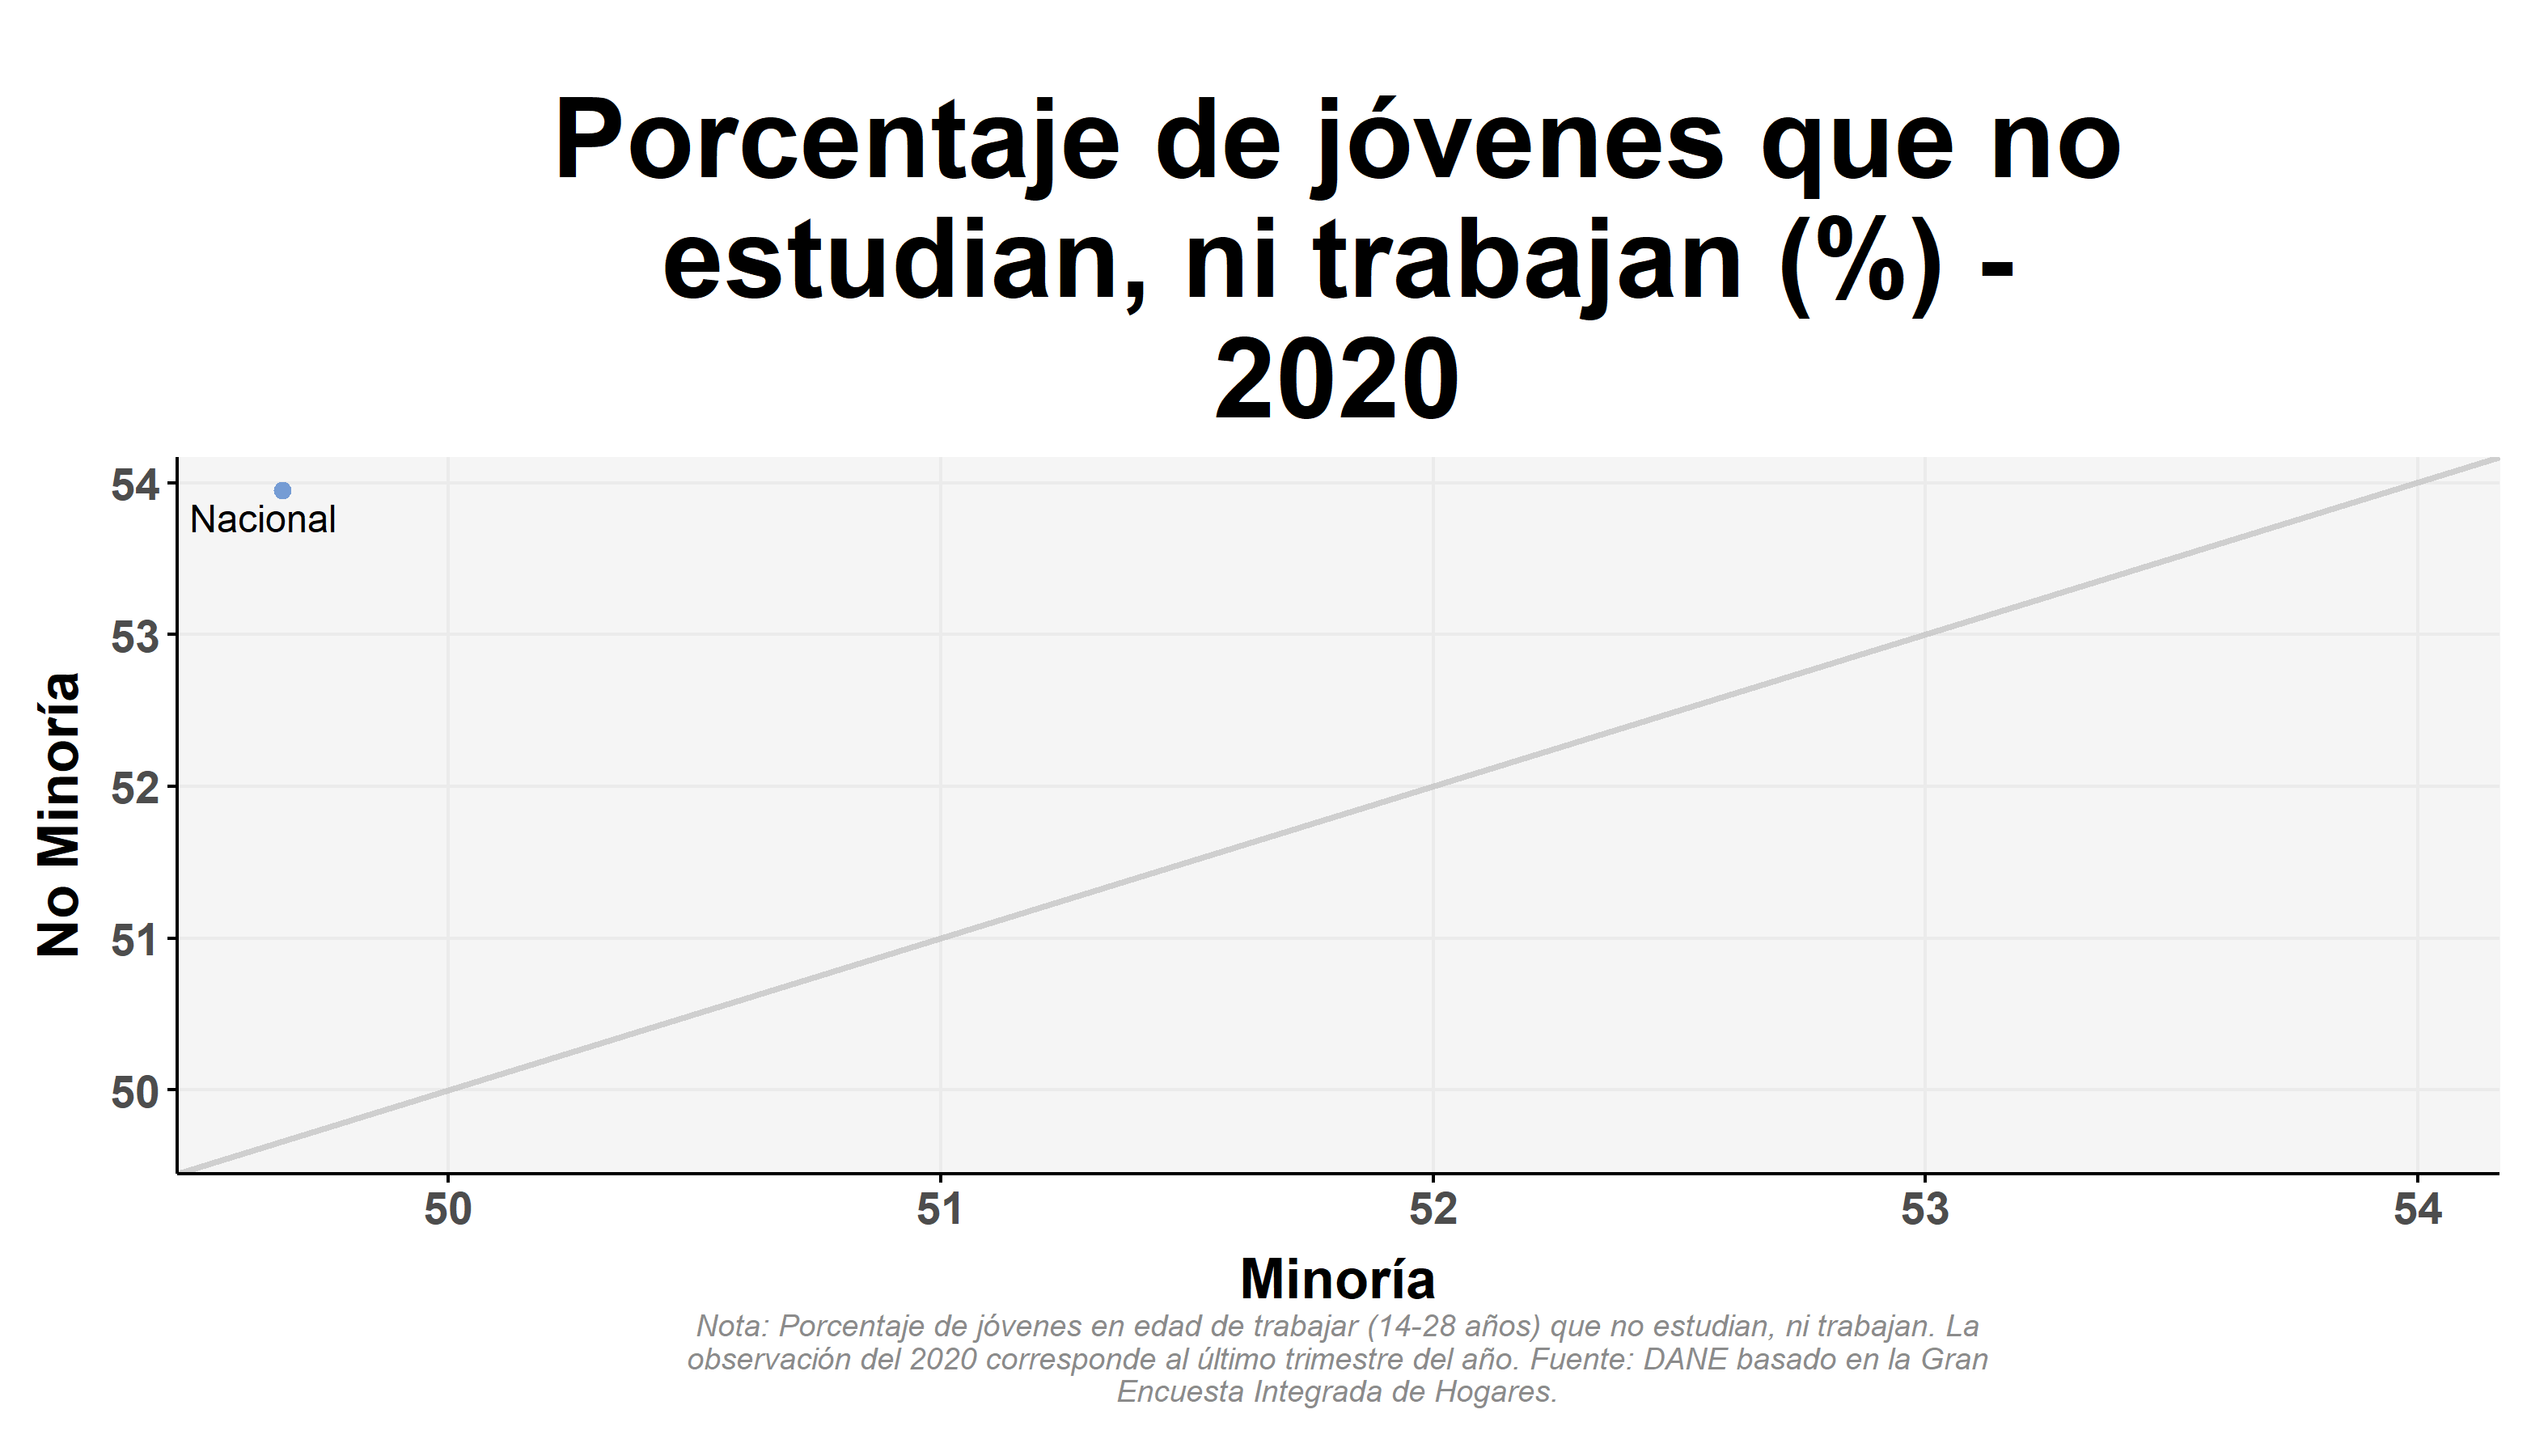
\includegraphics[width=\textwidth,keepaspectratio]{img/var_40_scatter.png}
        \end{center}
    \end{figure}
            \begin{itemize}
                \item El porcentaje de ninis jóvenes es mayor para las no minorías, aunque la diferencia es de poco más de un 4\%, siendo para las minorías un 54\% y las no minorías cerca del 50\%.
                \item En ambas desagregaciones vemos que la mitad de los jóvenes no estudian ni trabajan.
                \end{itemize}

        \subsubsection{Tasa de desempleo joven}

%%%% Include figures
    \begin{figure}[H]
        \caption{Tasa de desempleo joven a nivel nacional \label{map_result_2} }
        \begin{center}
        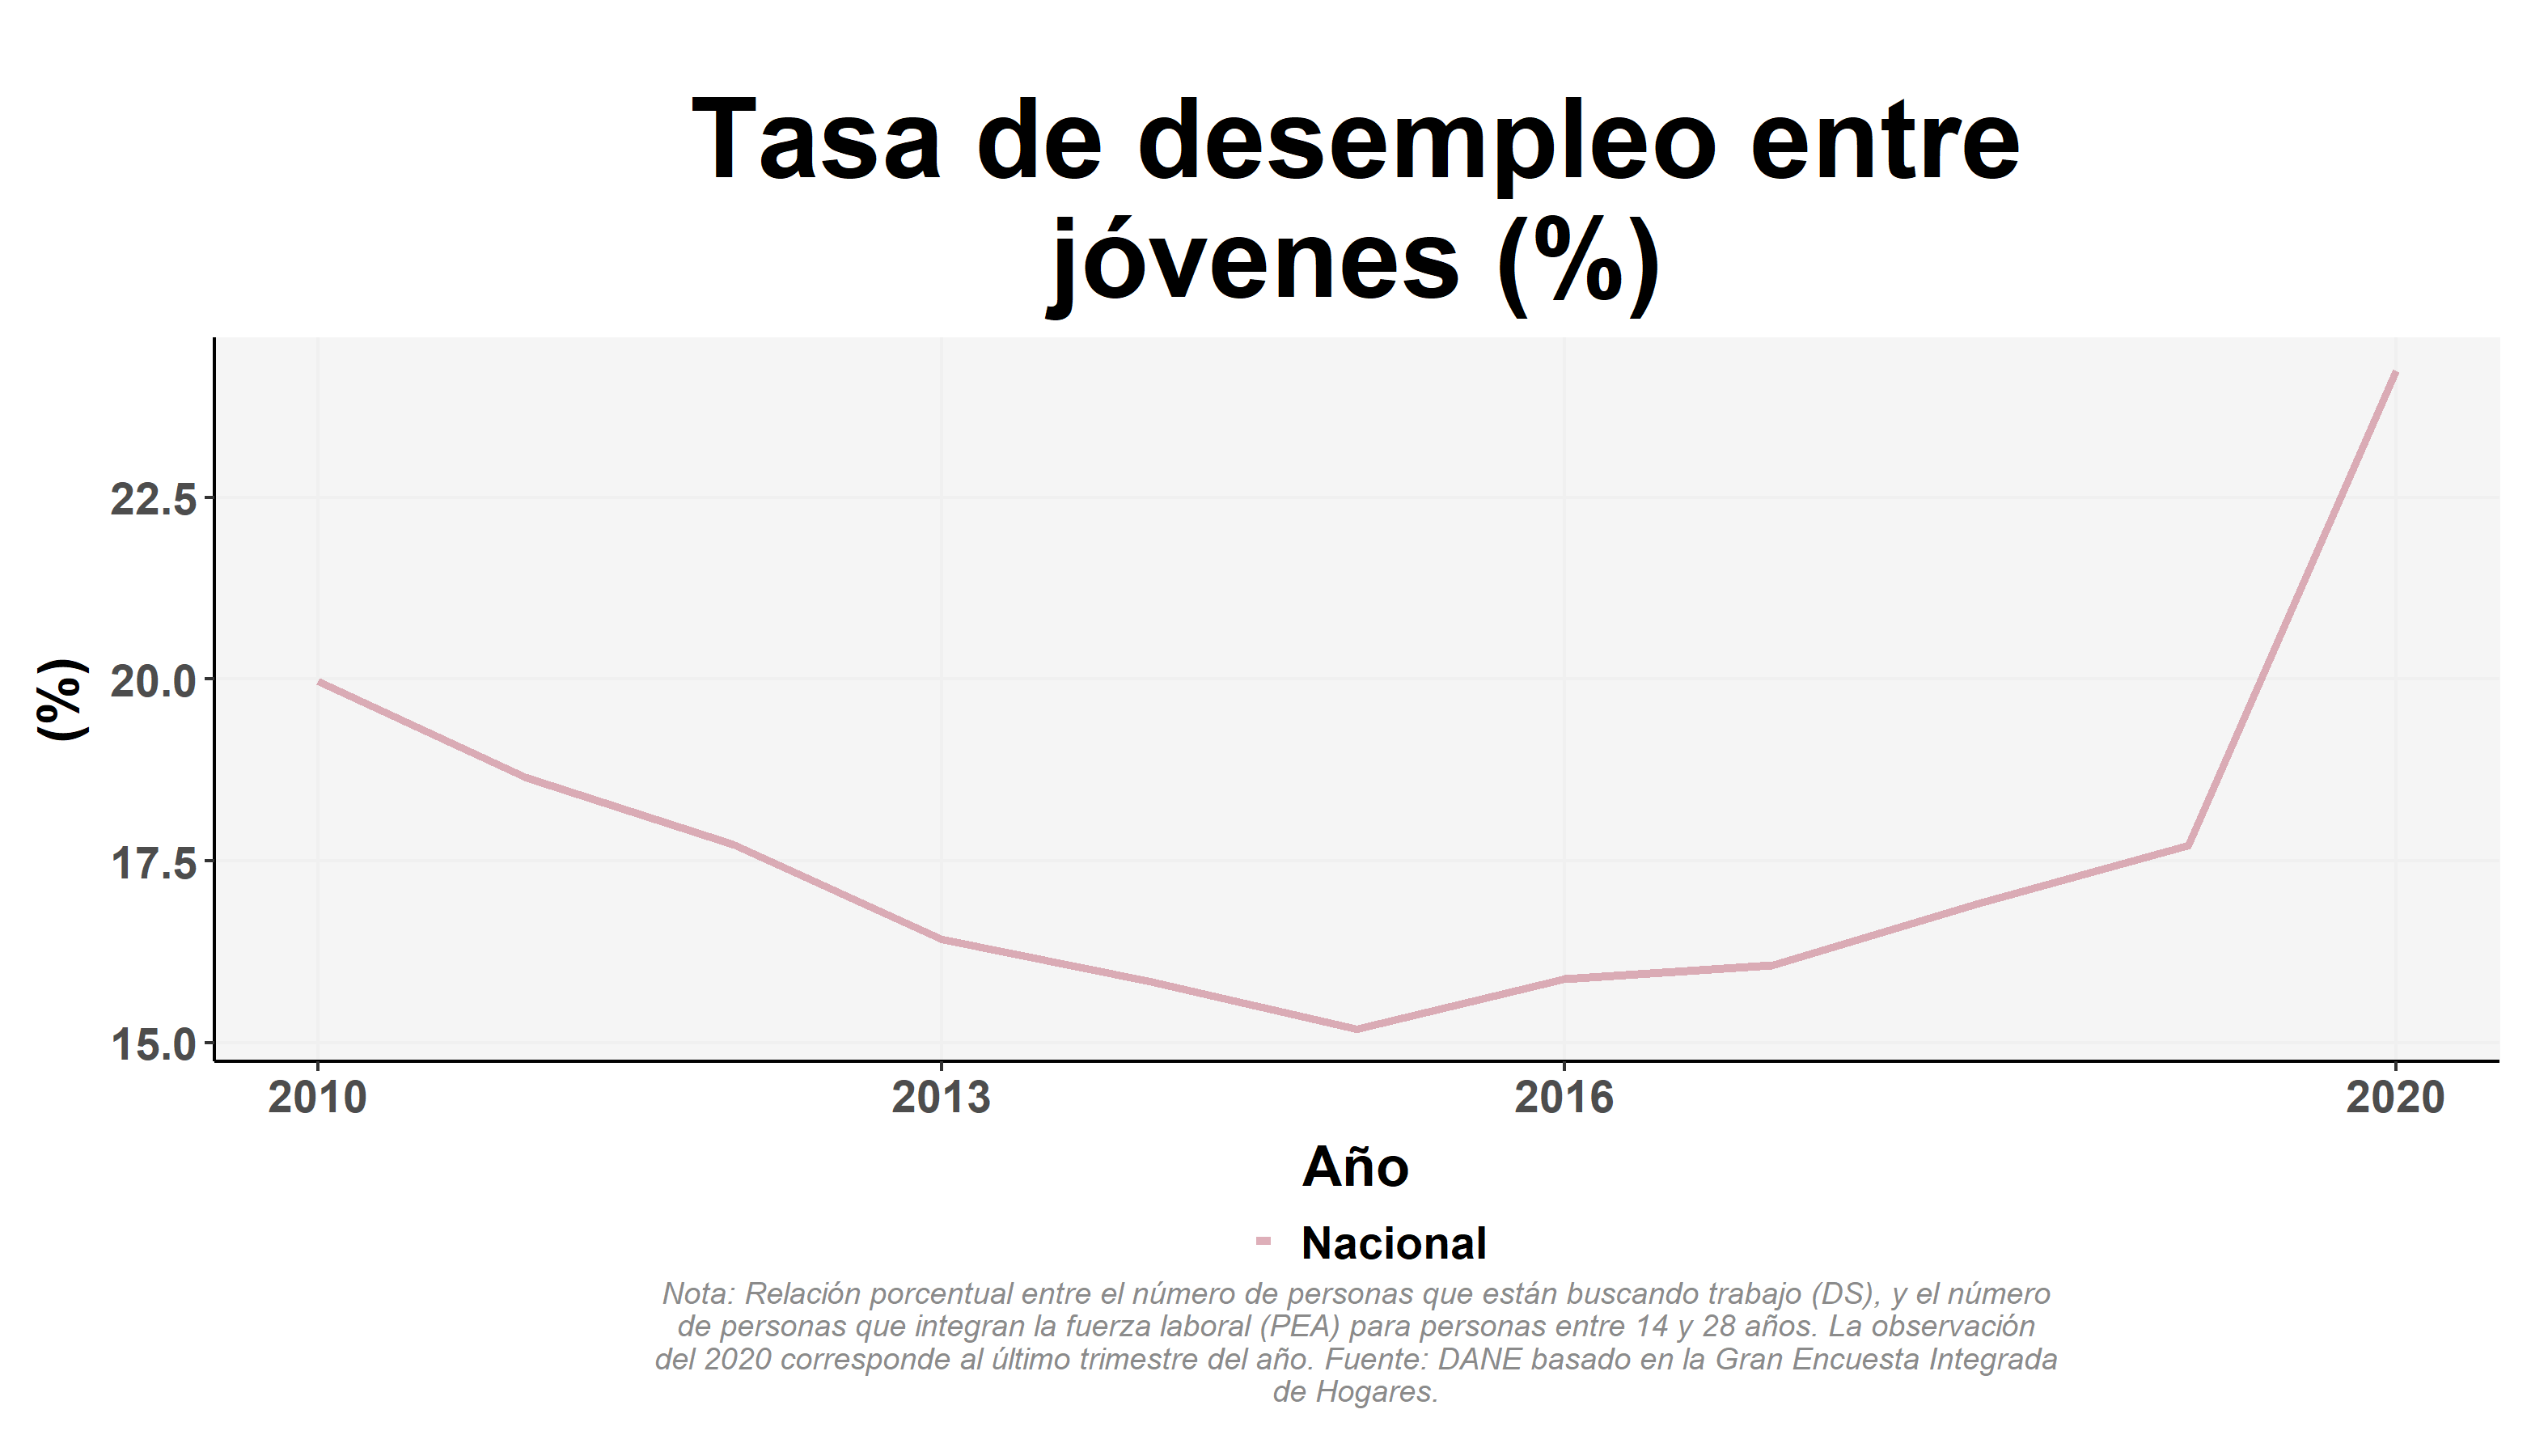
\includegraphics[width=\textwidth,keepaspectratio]{img/var_56_trend.png}
        \end{center}
    \end{figure}
            \begin{itemize}
                \item En la primera mitad de la década se evidencio una disminución de la tasa de desempleo para los jóvenes, pero a partir del 2016 esta volvió a incrementar.
                \item Para 2020 vemos que la tasa de desempleo tuvo un fuerte aumento, cambiando la tendencia que traía, que llevó a registrar una tasa superior a la de 11 años atrás.
                \end{itemize}

%%%% Include figures
    \begin{figure}[H]
        \caption{Tasa de desempleo joven por género \label{map_result_2} }
        \begin{center}
        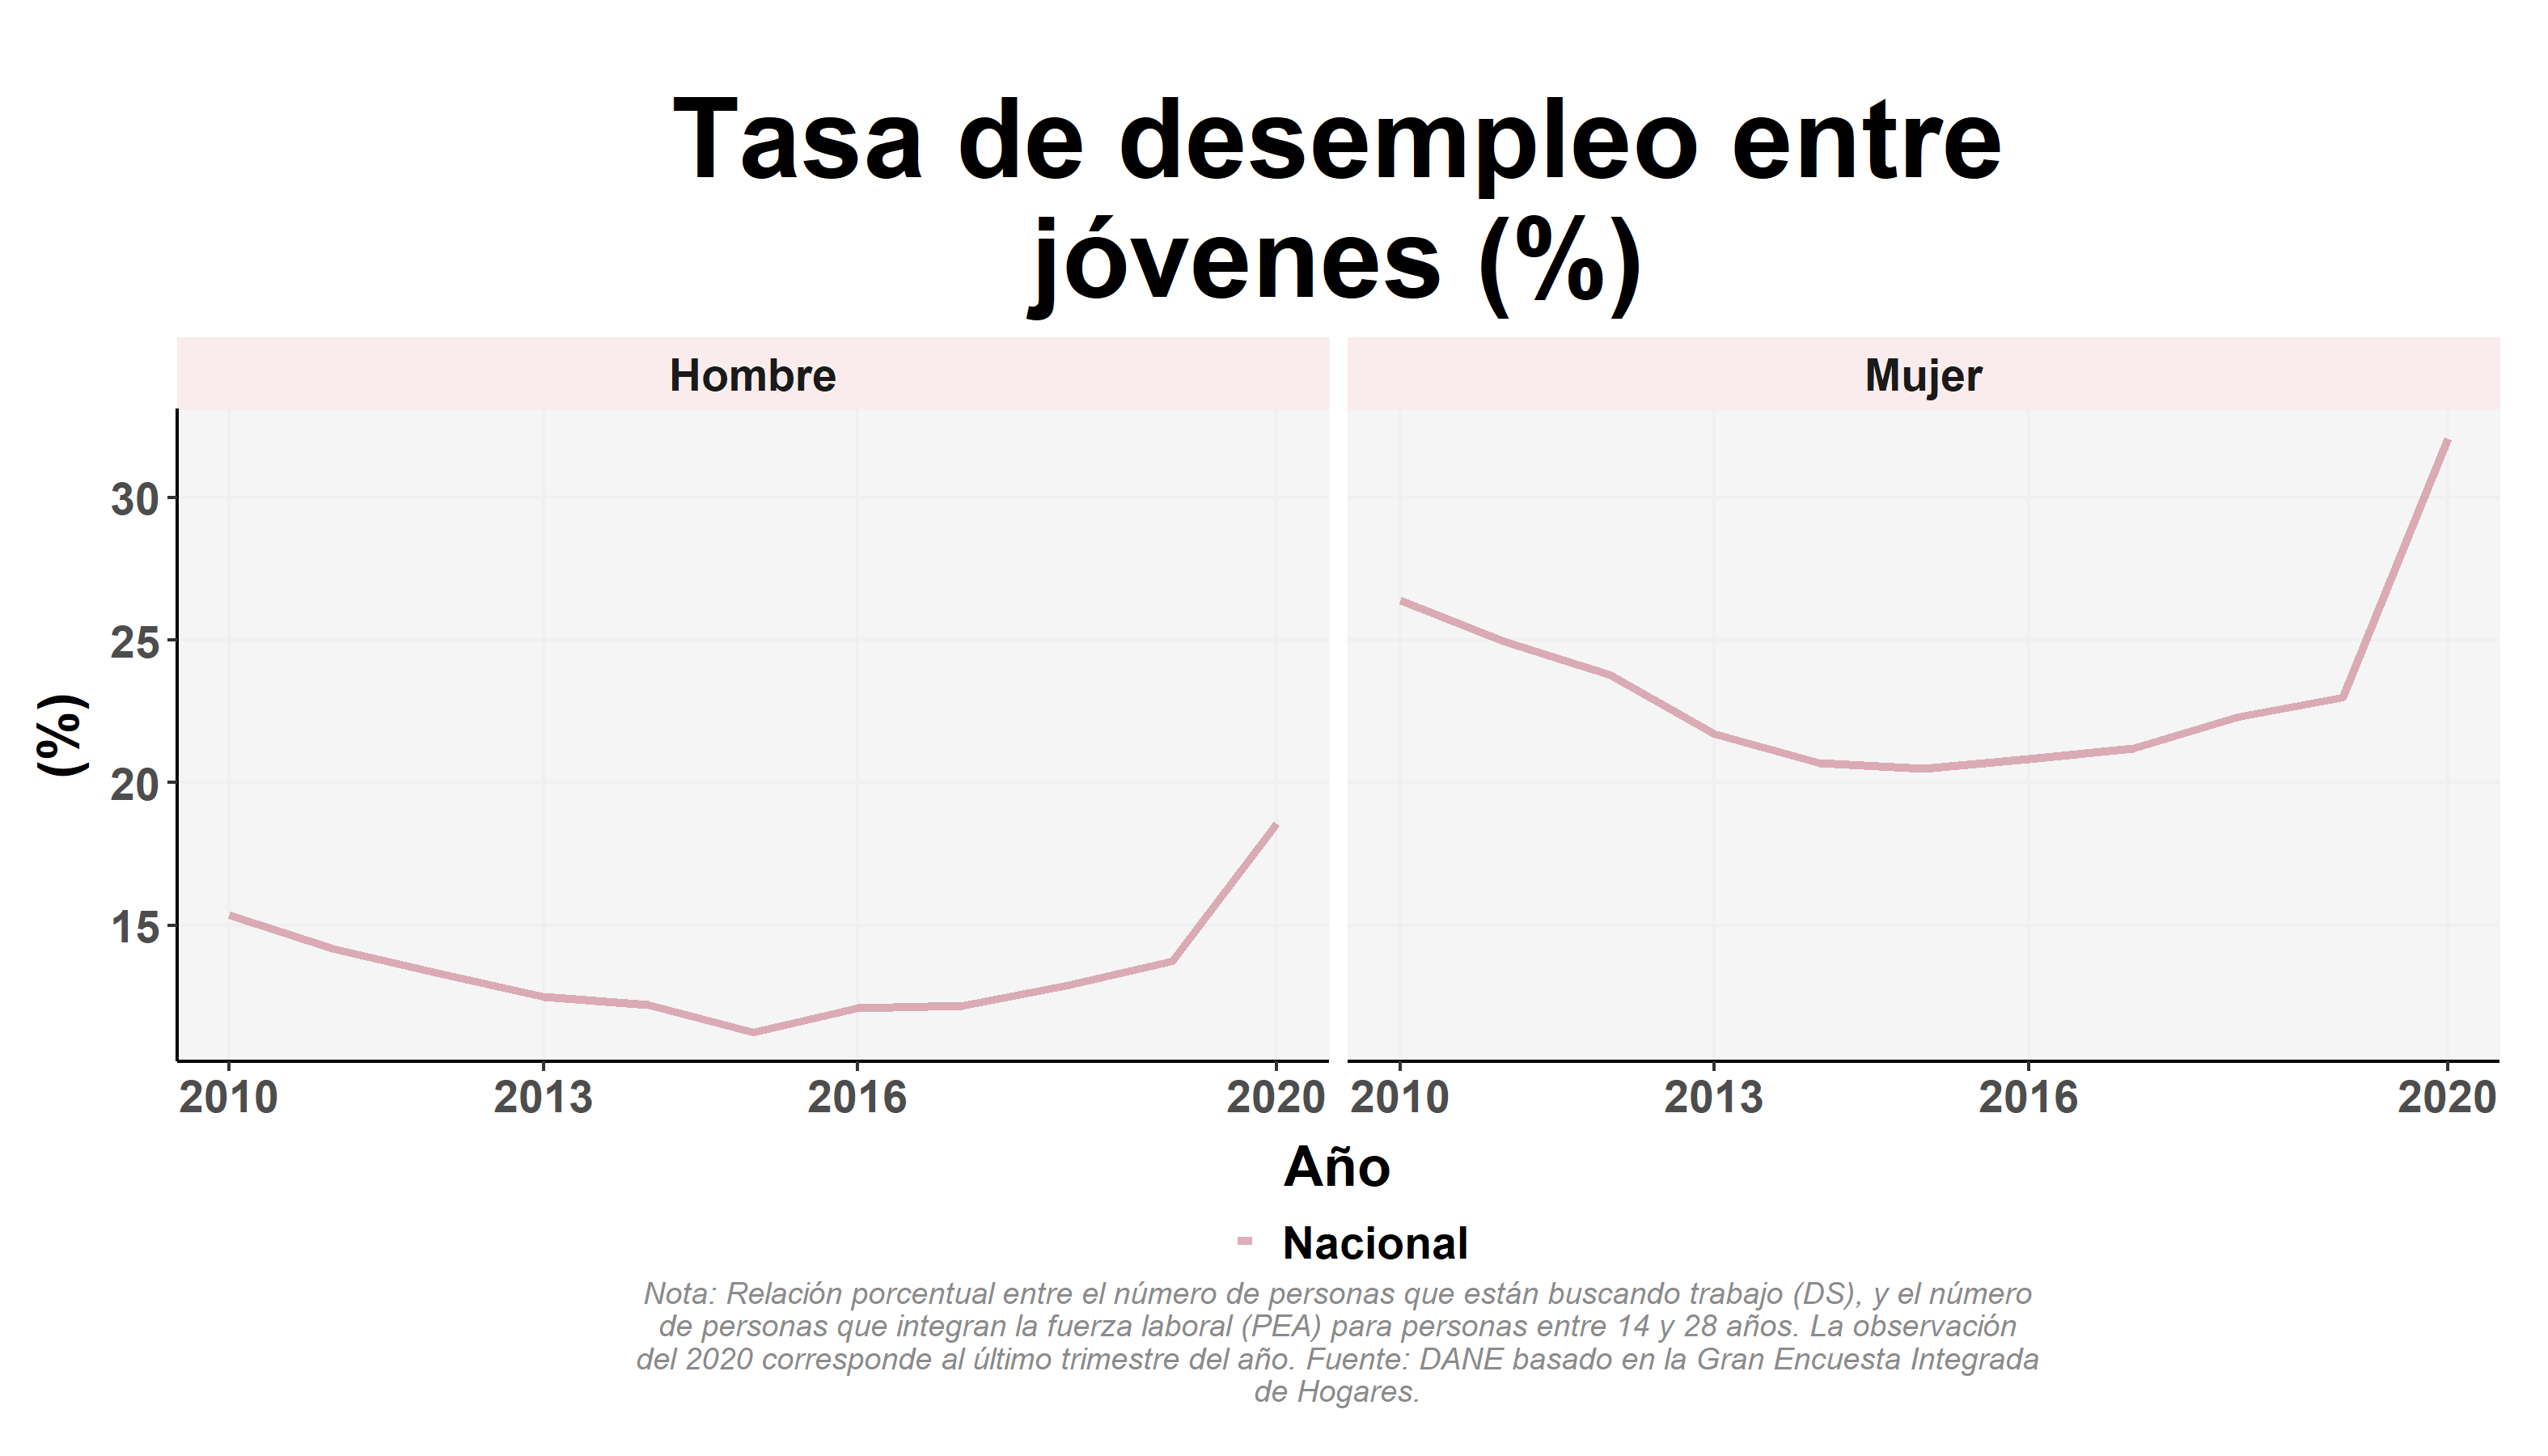
\includegraphics[width=\textwidth,keepaspectratio]{img/var_55_trend.png}
        \end{center}
    \end{figure}
            \begin{itemize}
                \item El desempleo tanto en hombre y mujeres jóvenes es mayor en 2020 de lo que era en el 2010.
                \item Existe una brecha de género, siendo la tasa de desempleo de la mujer más alta en aproximadamente un 10\% con respecto a la del hombre.
                \item Los cambios en la tendencia es mayor en la mujer, por eso aunque ambos tuvieron un aumento en 2020 por la pandemia, la tasa de la mujer fue más afectada.
                \end{itemize}

%%%% Include figures
    \begin{figure}[H]
        \caption{Tasa de desempleo joven por minorías y no minorías para 2020 \label{map_result_2} }
        \begin{center}
        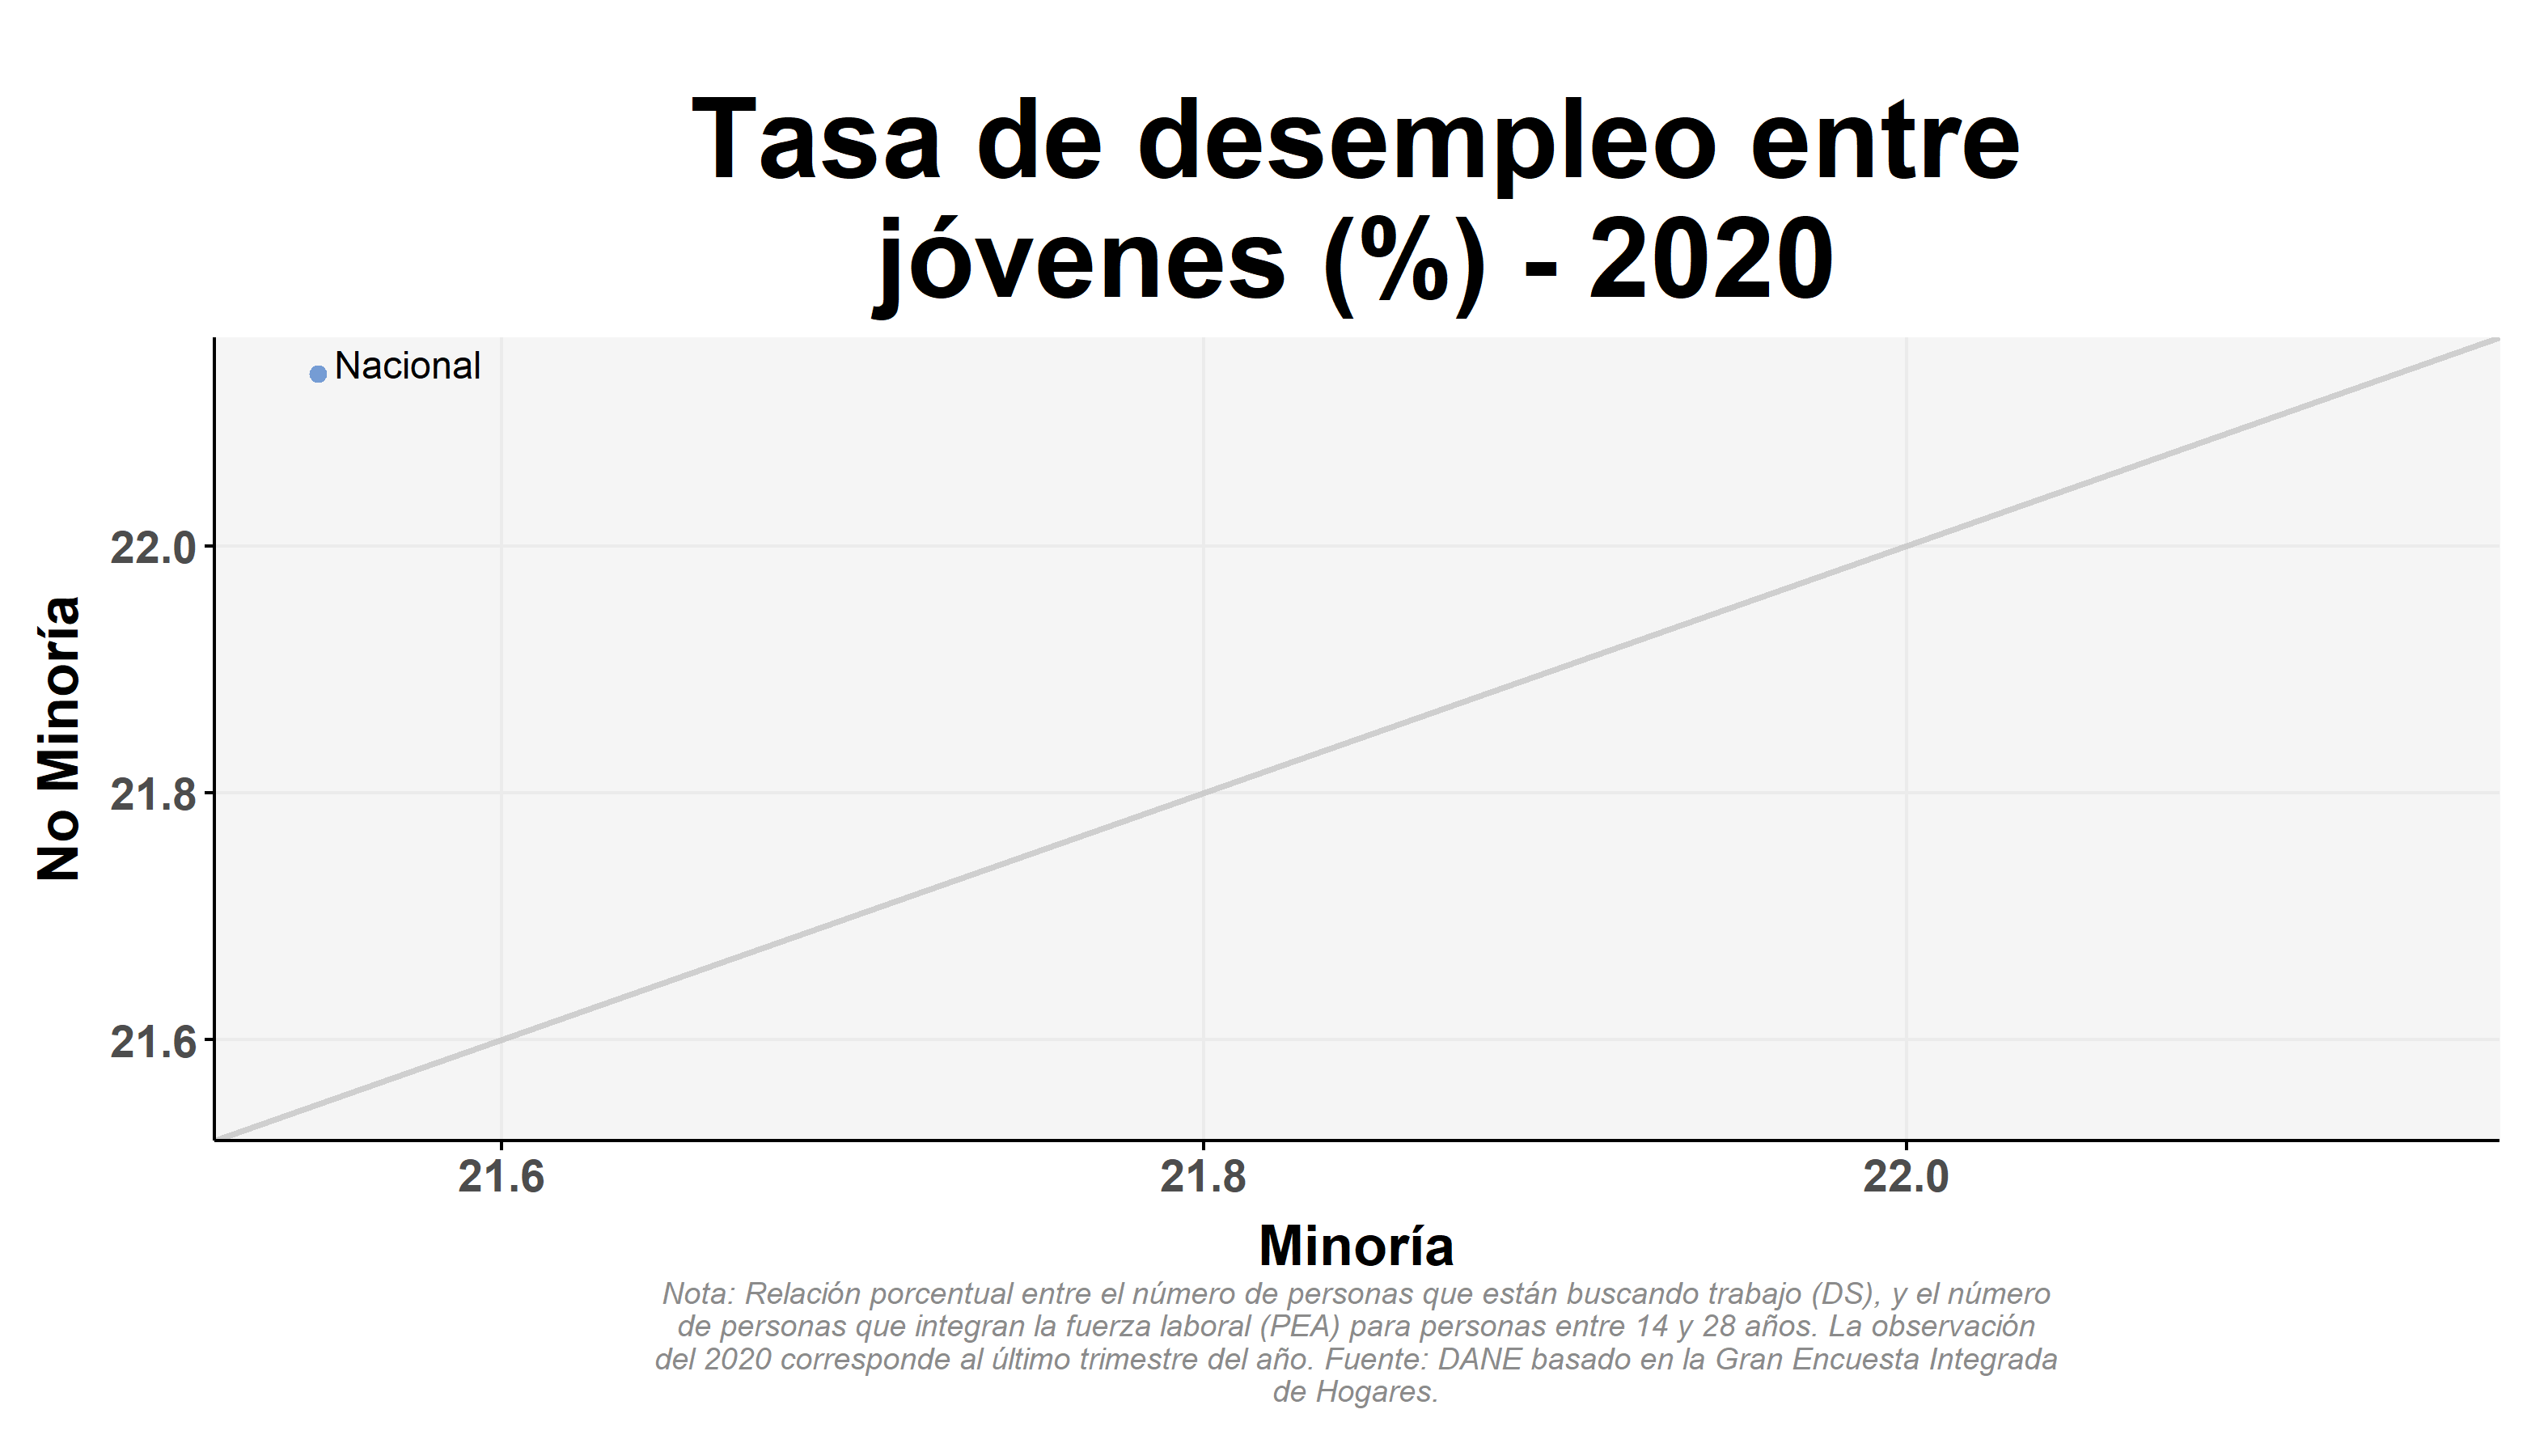
\includegraphics[width=\textwidth,keepaspectratio]{img/var_54_scatter.png}
        \end{center}
    \end{figure}
            \begin{itemize}
                \item Para 2020 las no minorías presentaron una mayor tasa de desempleo que las minorías, aunque la diferencia es de menos del 1\%.
                \end{itemize}

        \subsubsection{Tasa global de participación de los jóvenes}

%%%% Include figures
    \begin{figure}[H]
        \caption{Tasa global de participación entre jóvenes a nivel nacional \label{map_result_2} }
        \begin{center}
        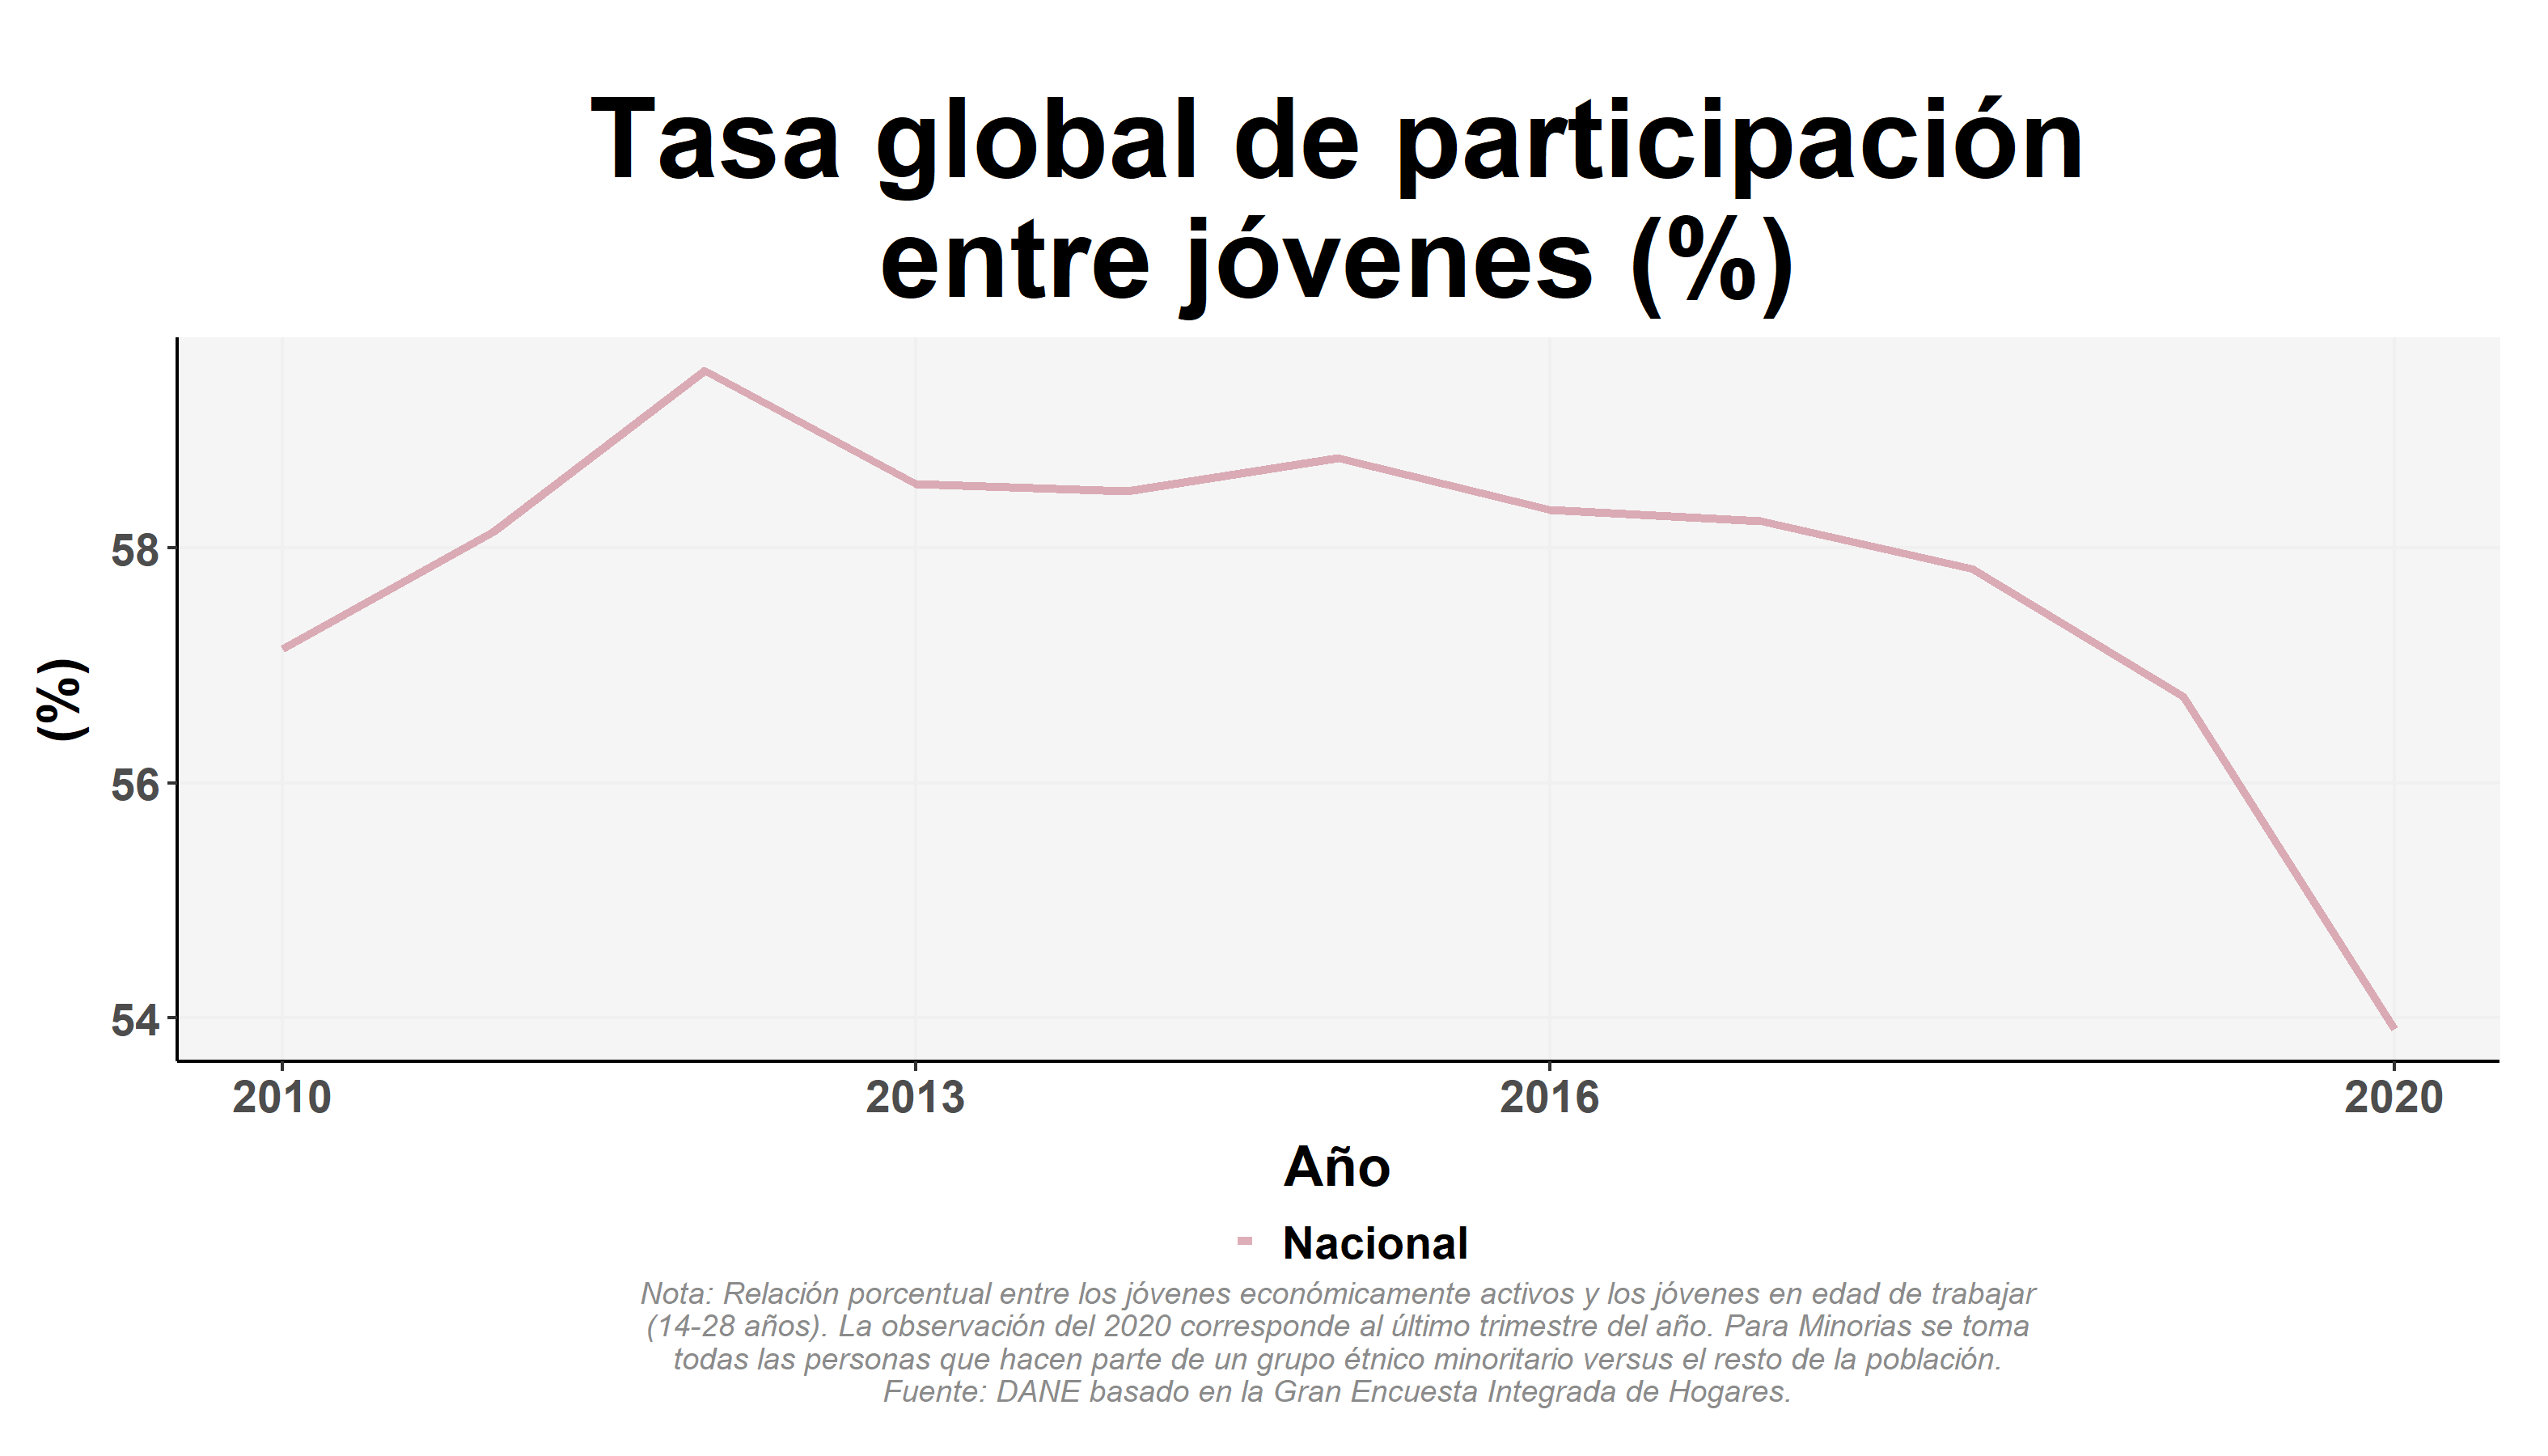
\includegraphics[width=\textwidth,keepaspectratio]{img/var_86_trend.png}
        \end{center}
    \end{figure}
            \begin{itemize}
                \item La tasa global de participación de jóvenes inició en la década con un aumento, pero desde 2013 ha venido disminuyendo de manera constante, intensificándose en 2020.
                \item En el 2020 la tasa de participación disminuyó significativamente a causa de la pandemia reportando valores menores que en el 2010, aunque cabe aclarar que desde el 2019 se había superado este valor.
                \end{itemize}

%%%% Include figures
    \begin{figure}[H]
        \caption{Tasa global de participación entre jóvenes por género \label{map_result_2} }
        \begin{center}
        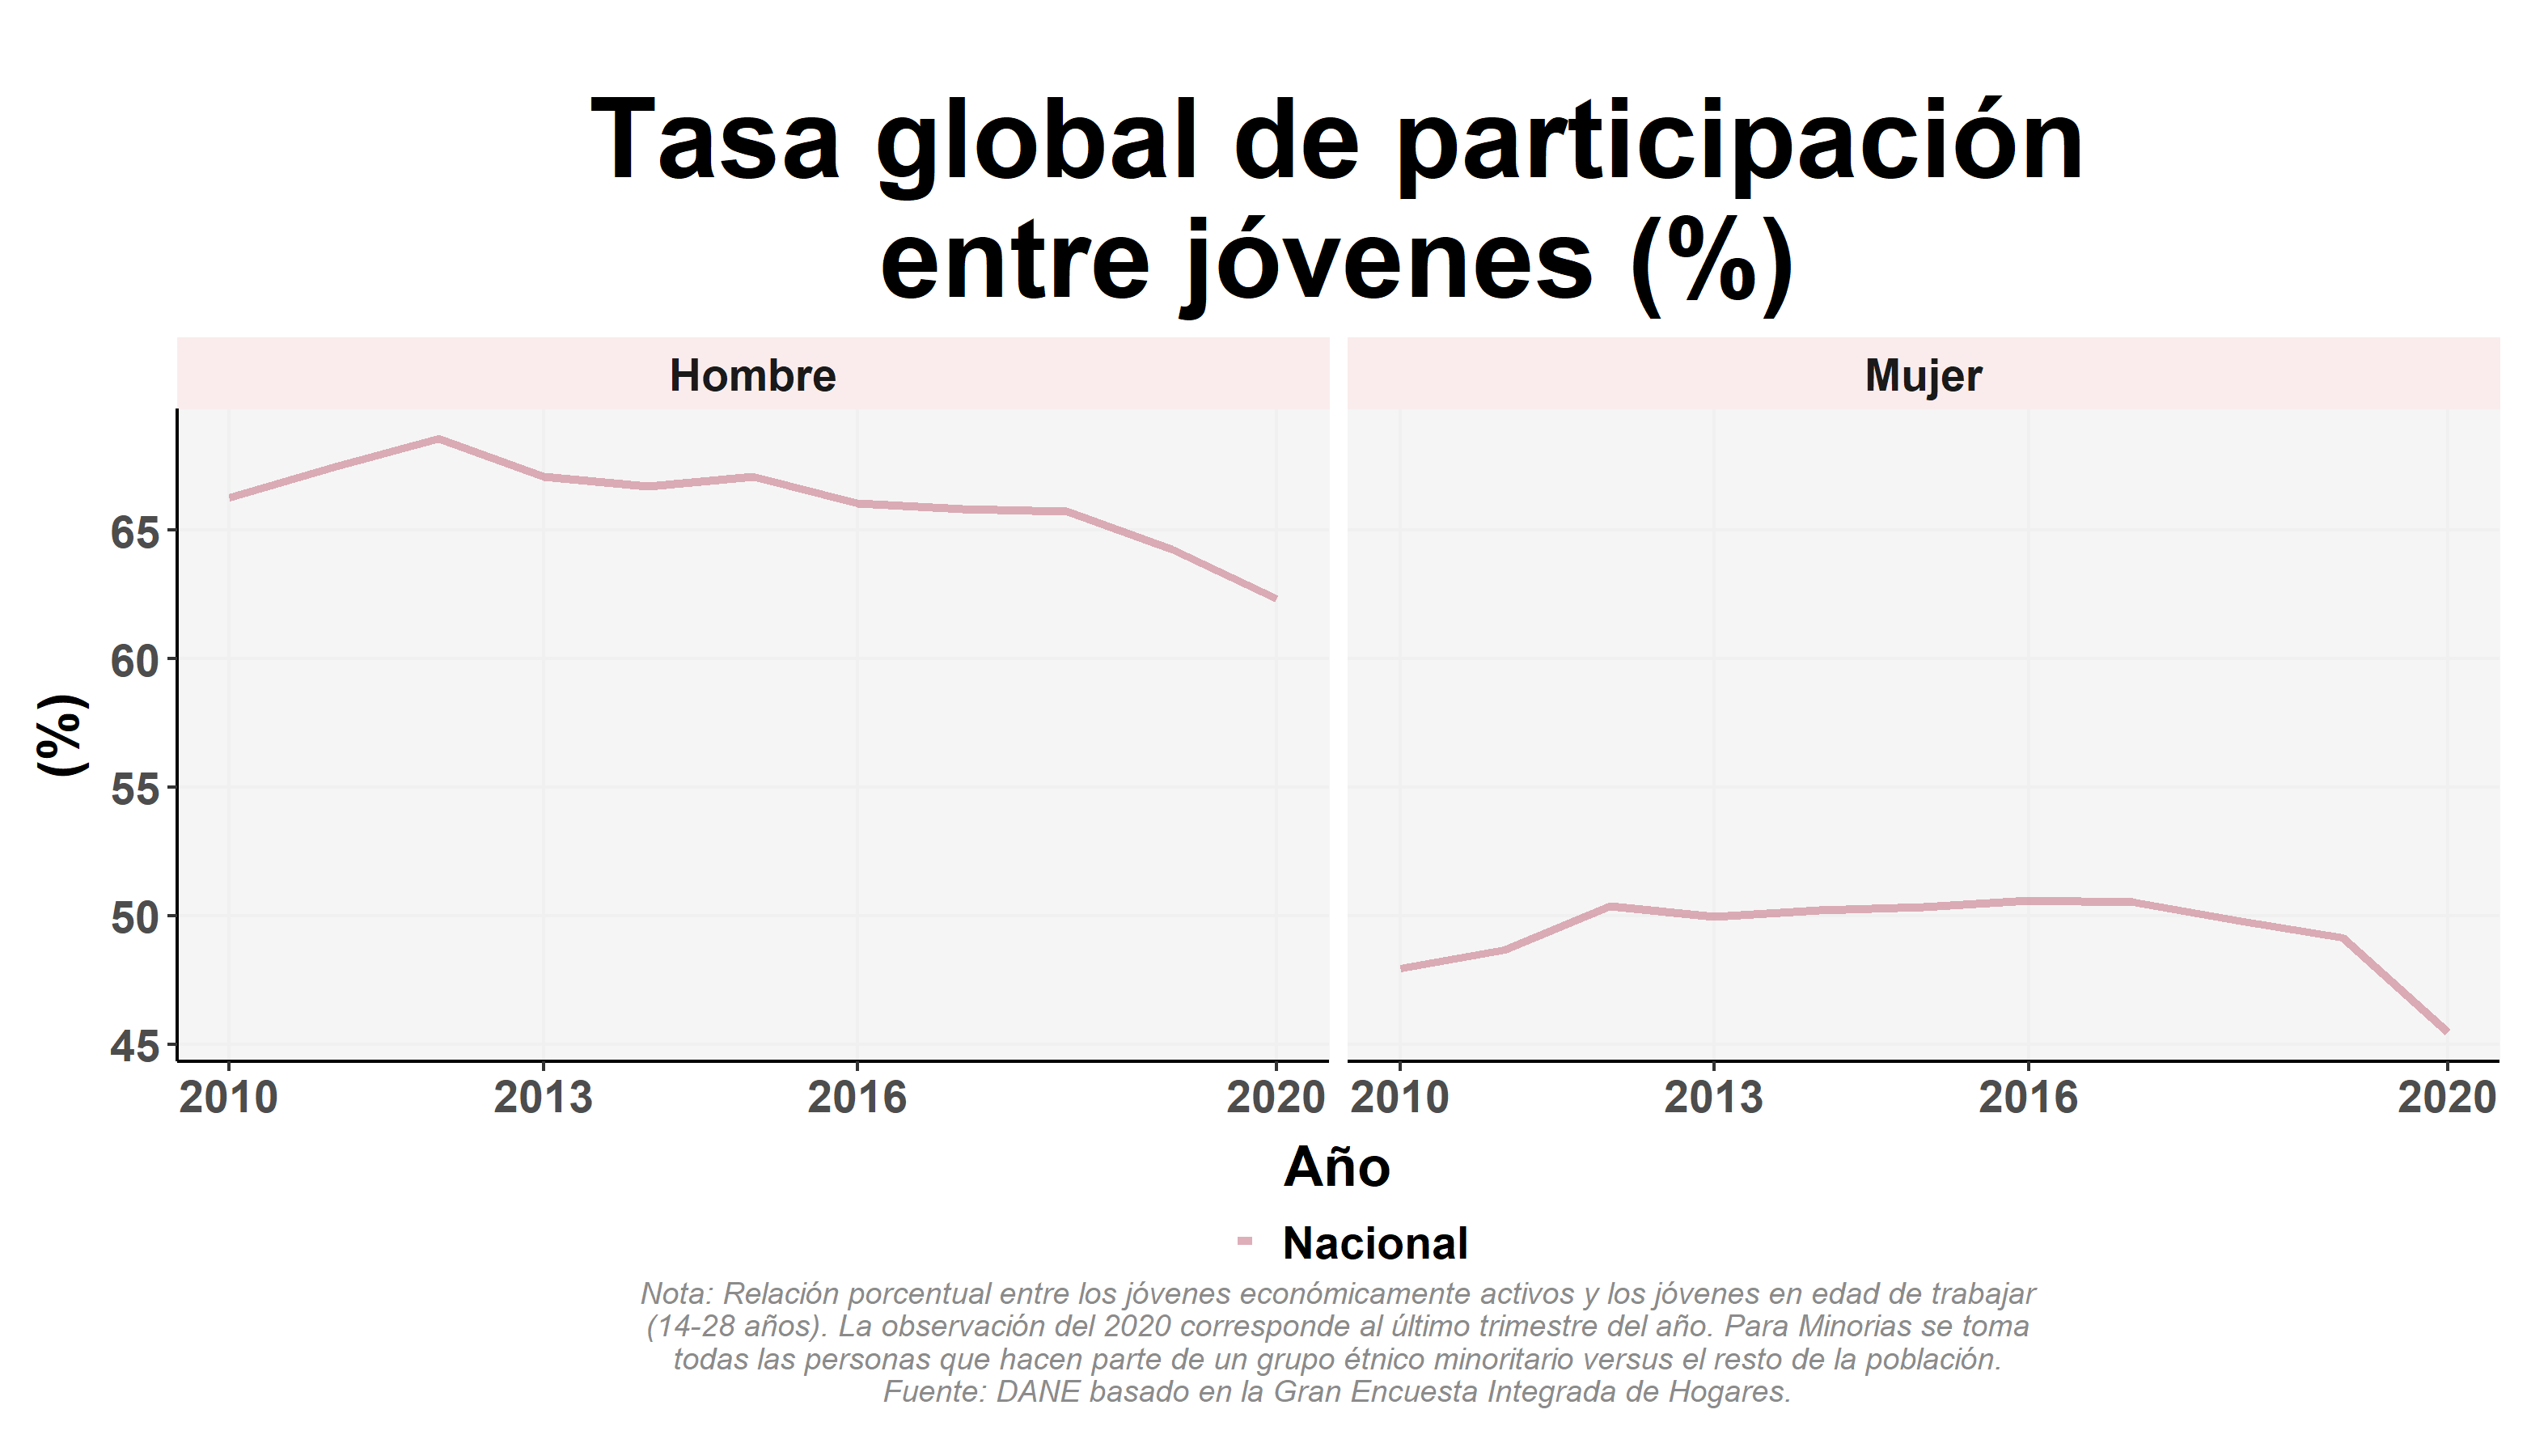
\includegraphics[width=\textwidth,keepaspectratio]{img/var_85_trend.png}
        \end{center}
    \end{figure}
            \begin{itemize}
                \item La participación laboral evidencia una brecha entre hombres y mujeres, siendo mayor la participación de los hombres.
                \item La tasa de participación en los hombres evidencia mayor variación en el tiempo, mientras que la de la mujer se ha mantenido aparentemente constante.
                \item Para 2020 aunque la tasa de participación parecía más constante, la pandemia afecto más a estas que los hombres con una mayor disminución.
                \end{itemize}

%%%% Include figures
    \begin{figure}[H]
        \caption{Tasa global de participación entre jóvenes por minorías y no minorías para 2020 \label{map_result_2} }
        \begin{center}
        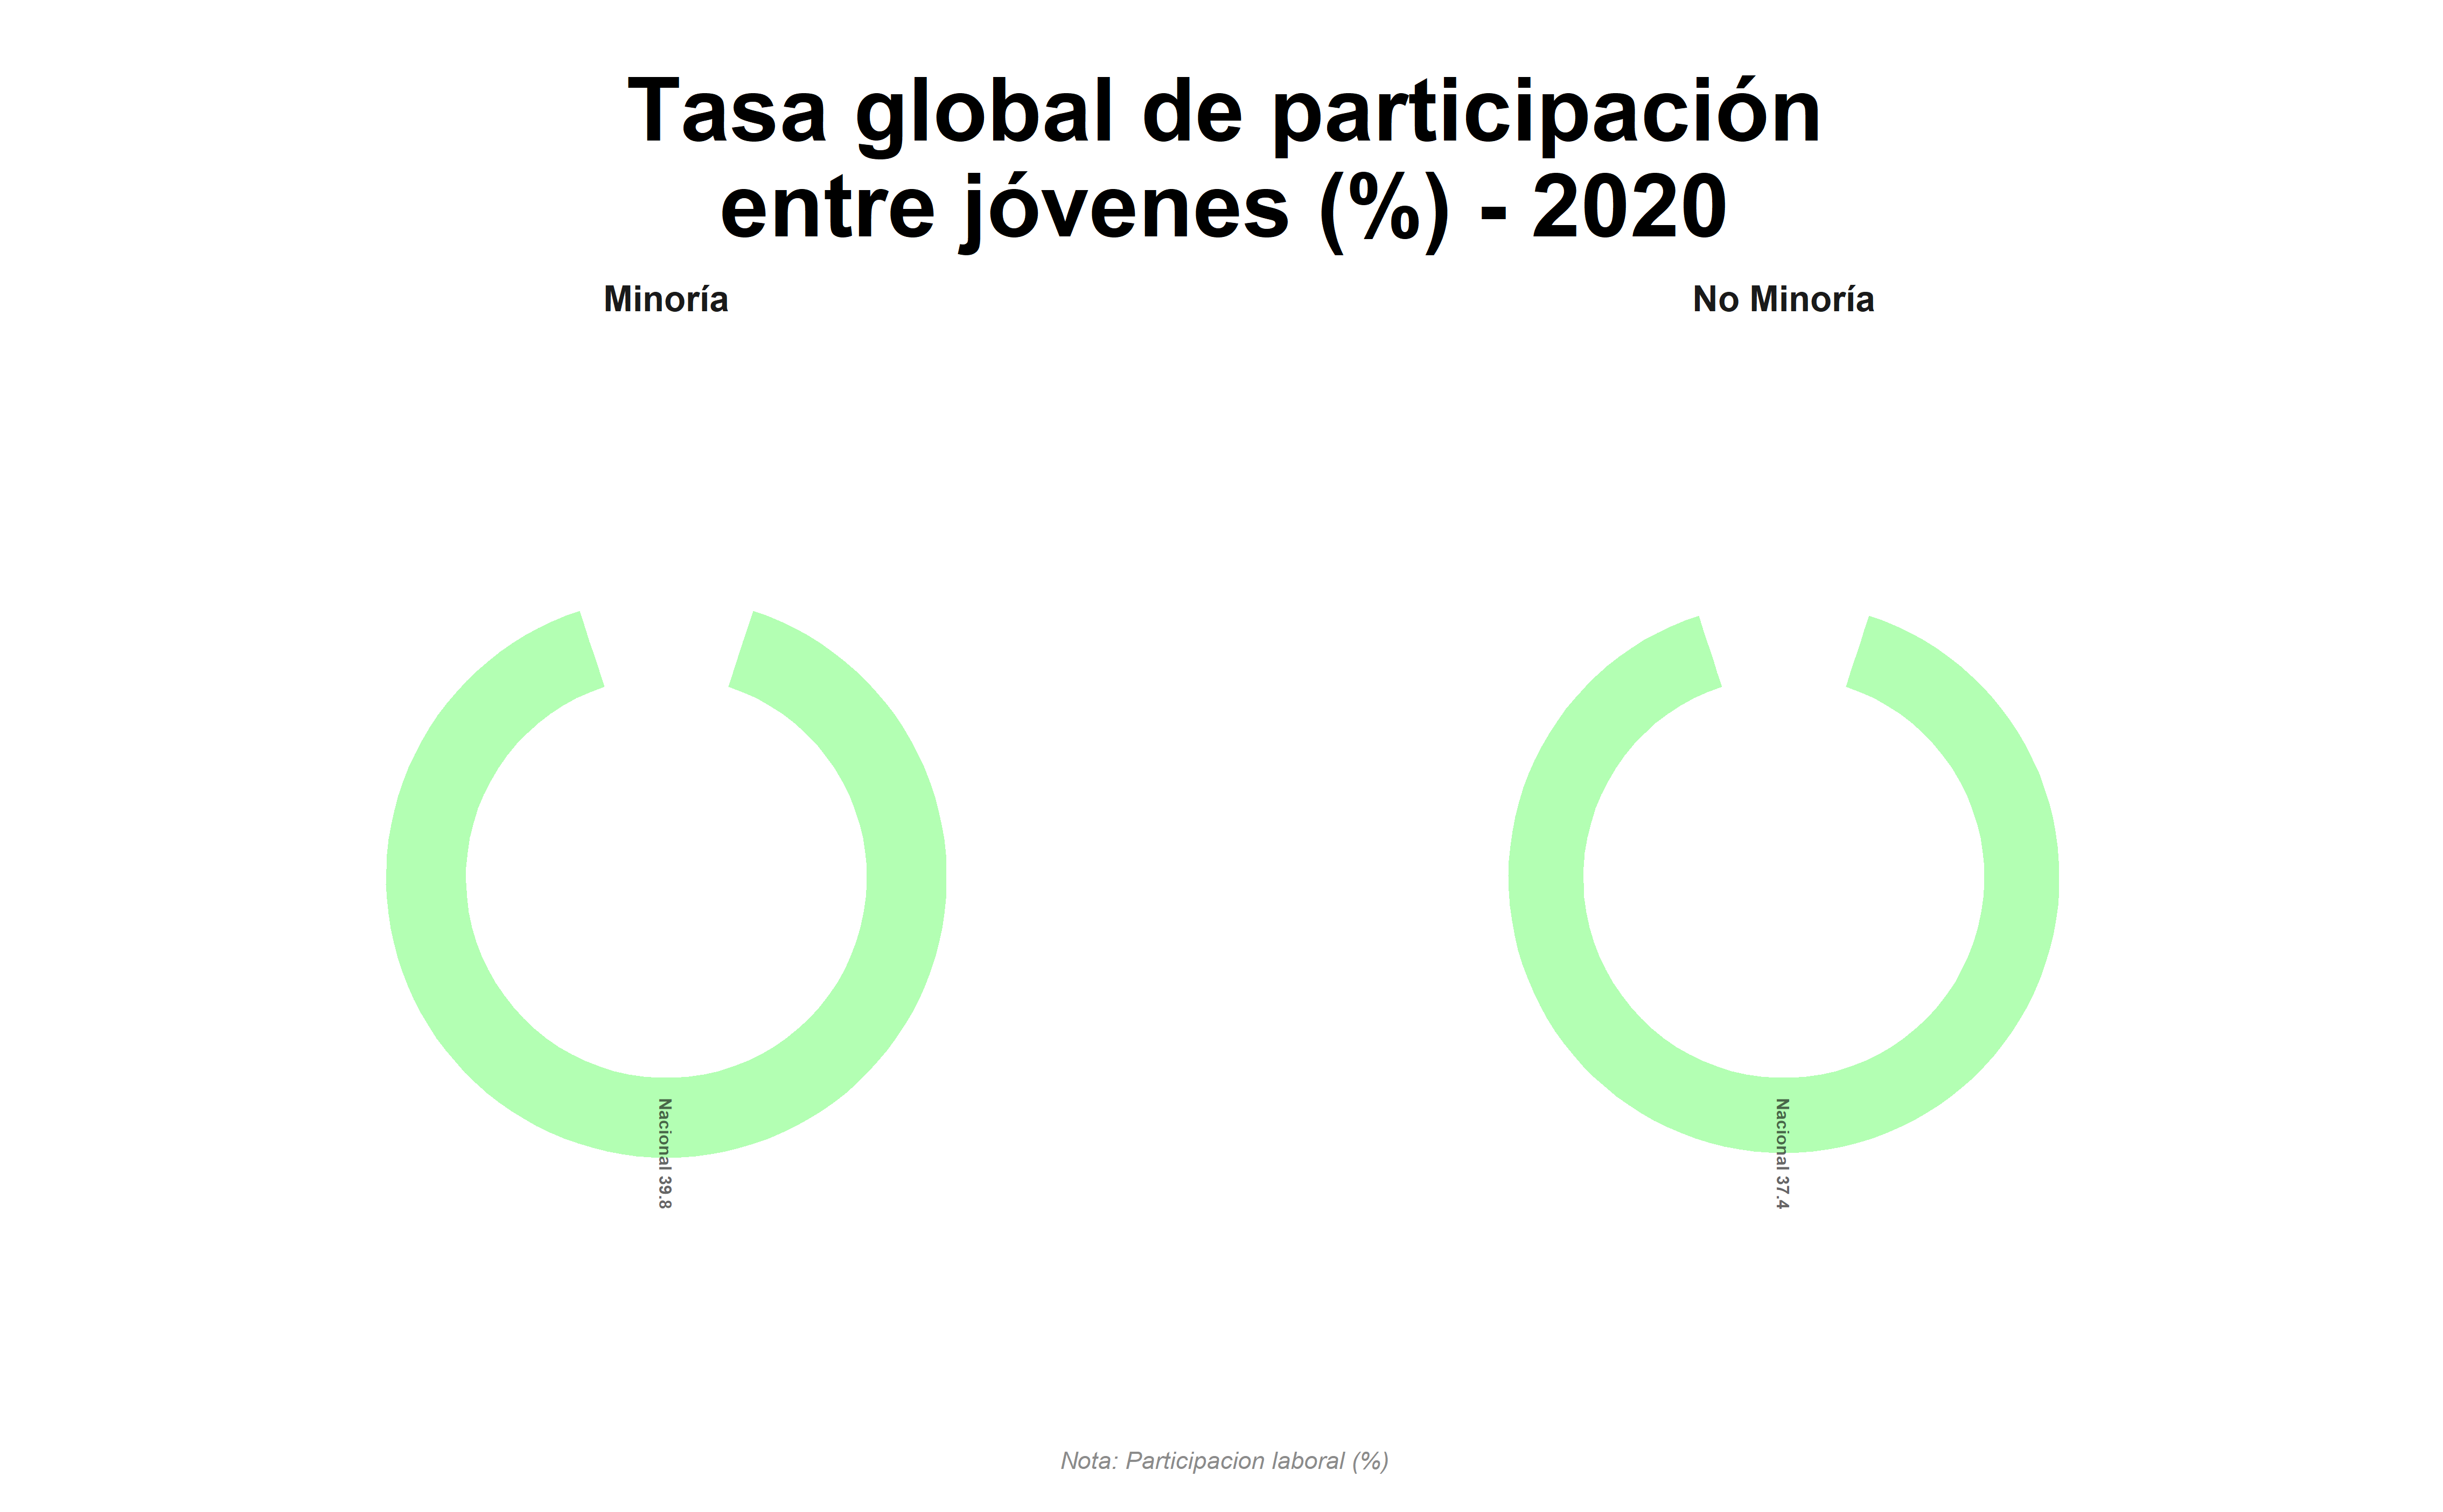
\includegraphics[width=\textwidth,keepaspectratio]{img/var_84_static.png}
        \end{center}
    \end{figure}
            \begin{itemize}
                \item La tasa global de participación es mayor para las minorías que para las no minorías.
                \item Hay una diferencia aproximadamente del 2\% entre las tasas de participación.
                \end{itemize}

    \subsection{Empleo formal}

%%%% Include figures
    \begin{figure}[H]
        \caption{Tasa de formalidad entre jóvenes a nivel nacional \label{map_result_2} }
        \begin{center}
        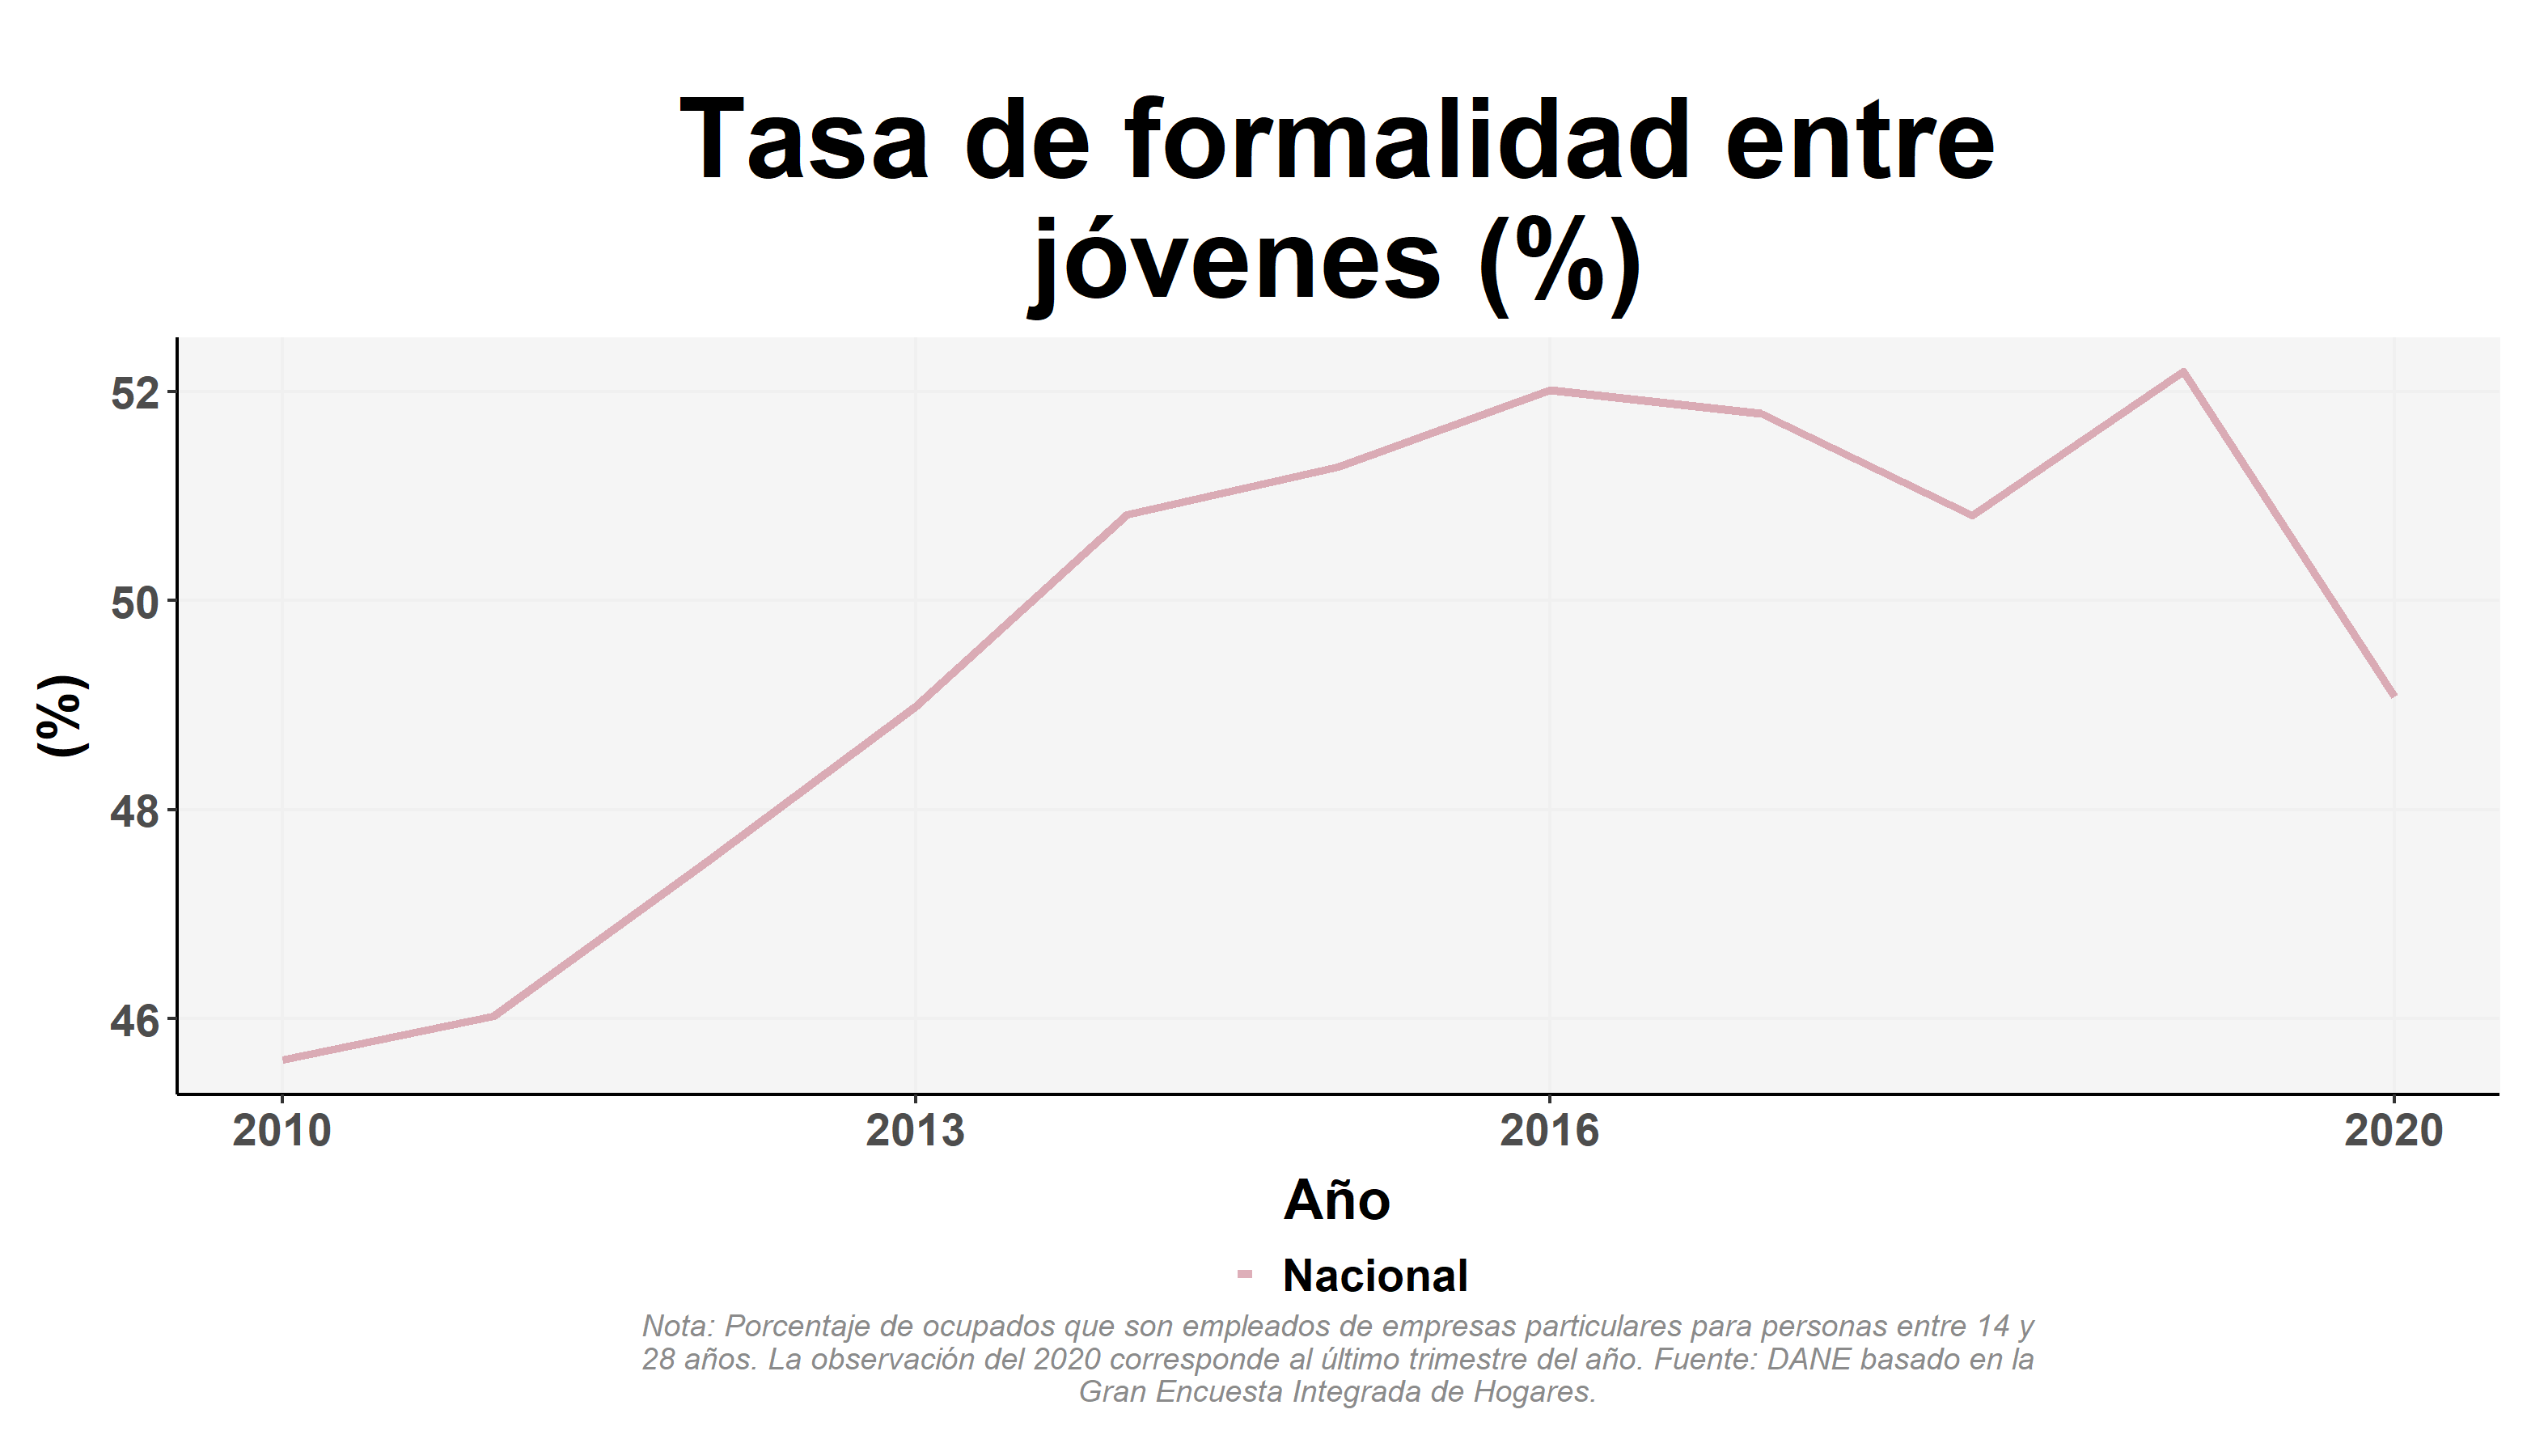
\includegraphics[width=\textwidth,keepaspectratio]{img/var_66_trend.png}
        \end{center}
    \end{figure}
            \begin{itemize}
                \item Hasta el 2016 la tasa de formalidad entre jóvenes estuvo en aumento, pero disminuyó a partir de ahí, presentando un pico en 2019 donde recuperó pero volvió a descender significativamente en 2020 a causa de la pandemia.
                \item Para 2020 la tasa de participación tuvo un retroceso de aproximadamente de 7 años, es decir que tenía niveles similares a los registrados en el 2013.
                \end{itemize}

%%%% Include figures
    \begin{figure}[H]
        \caption{Tasa de formalidad entre jóvenes por género \label{map_result_2} }
        \begin{center}
        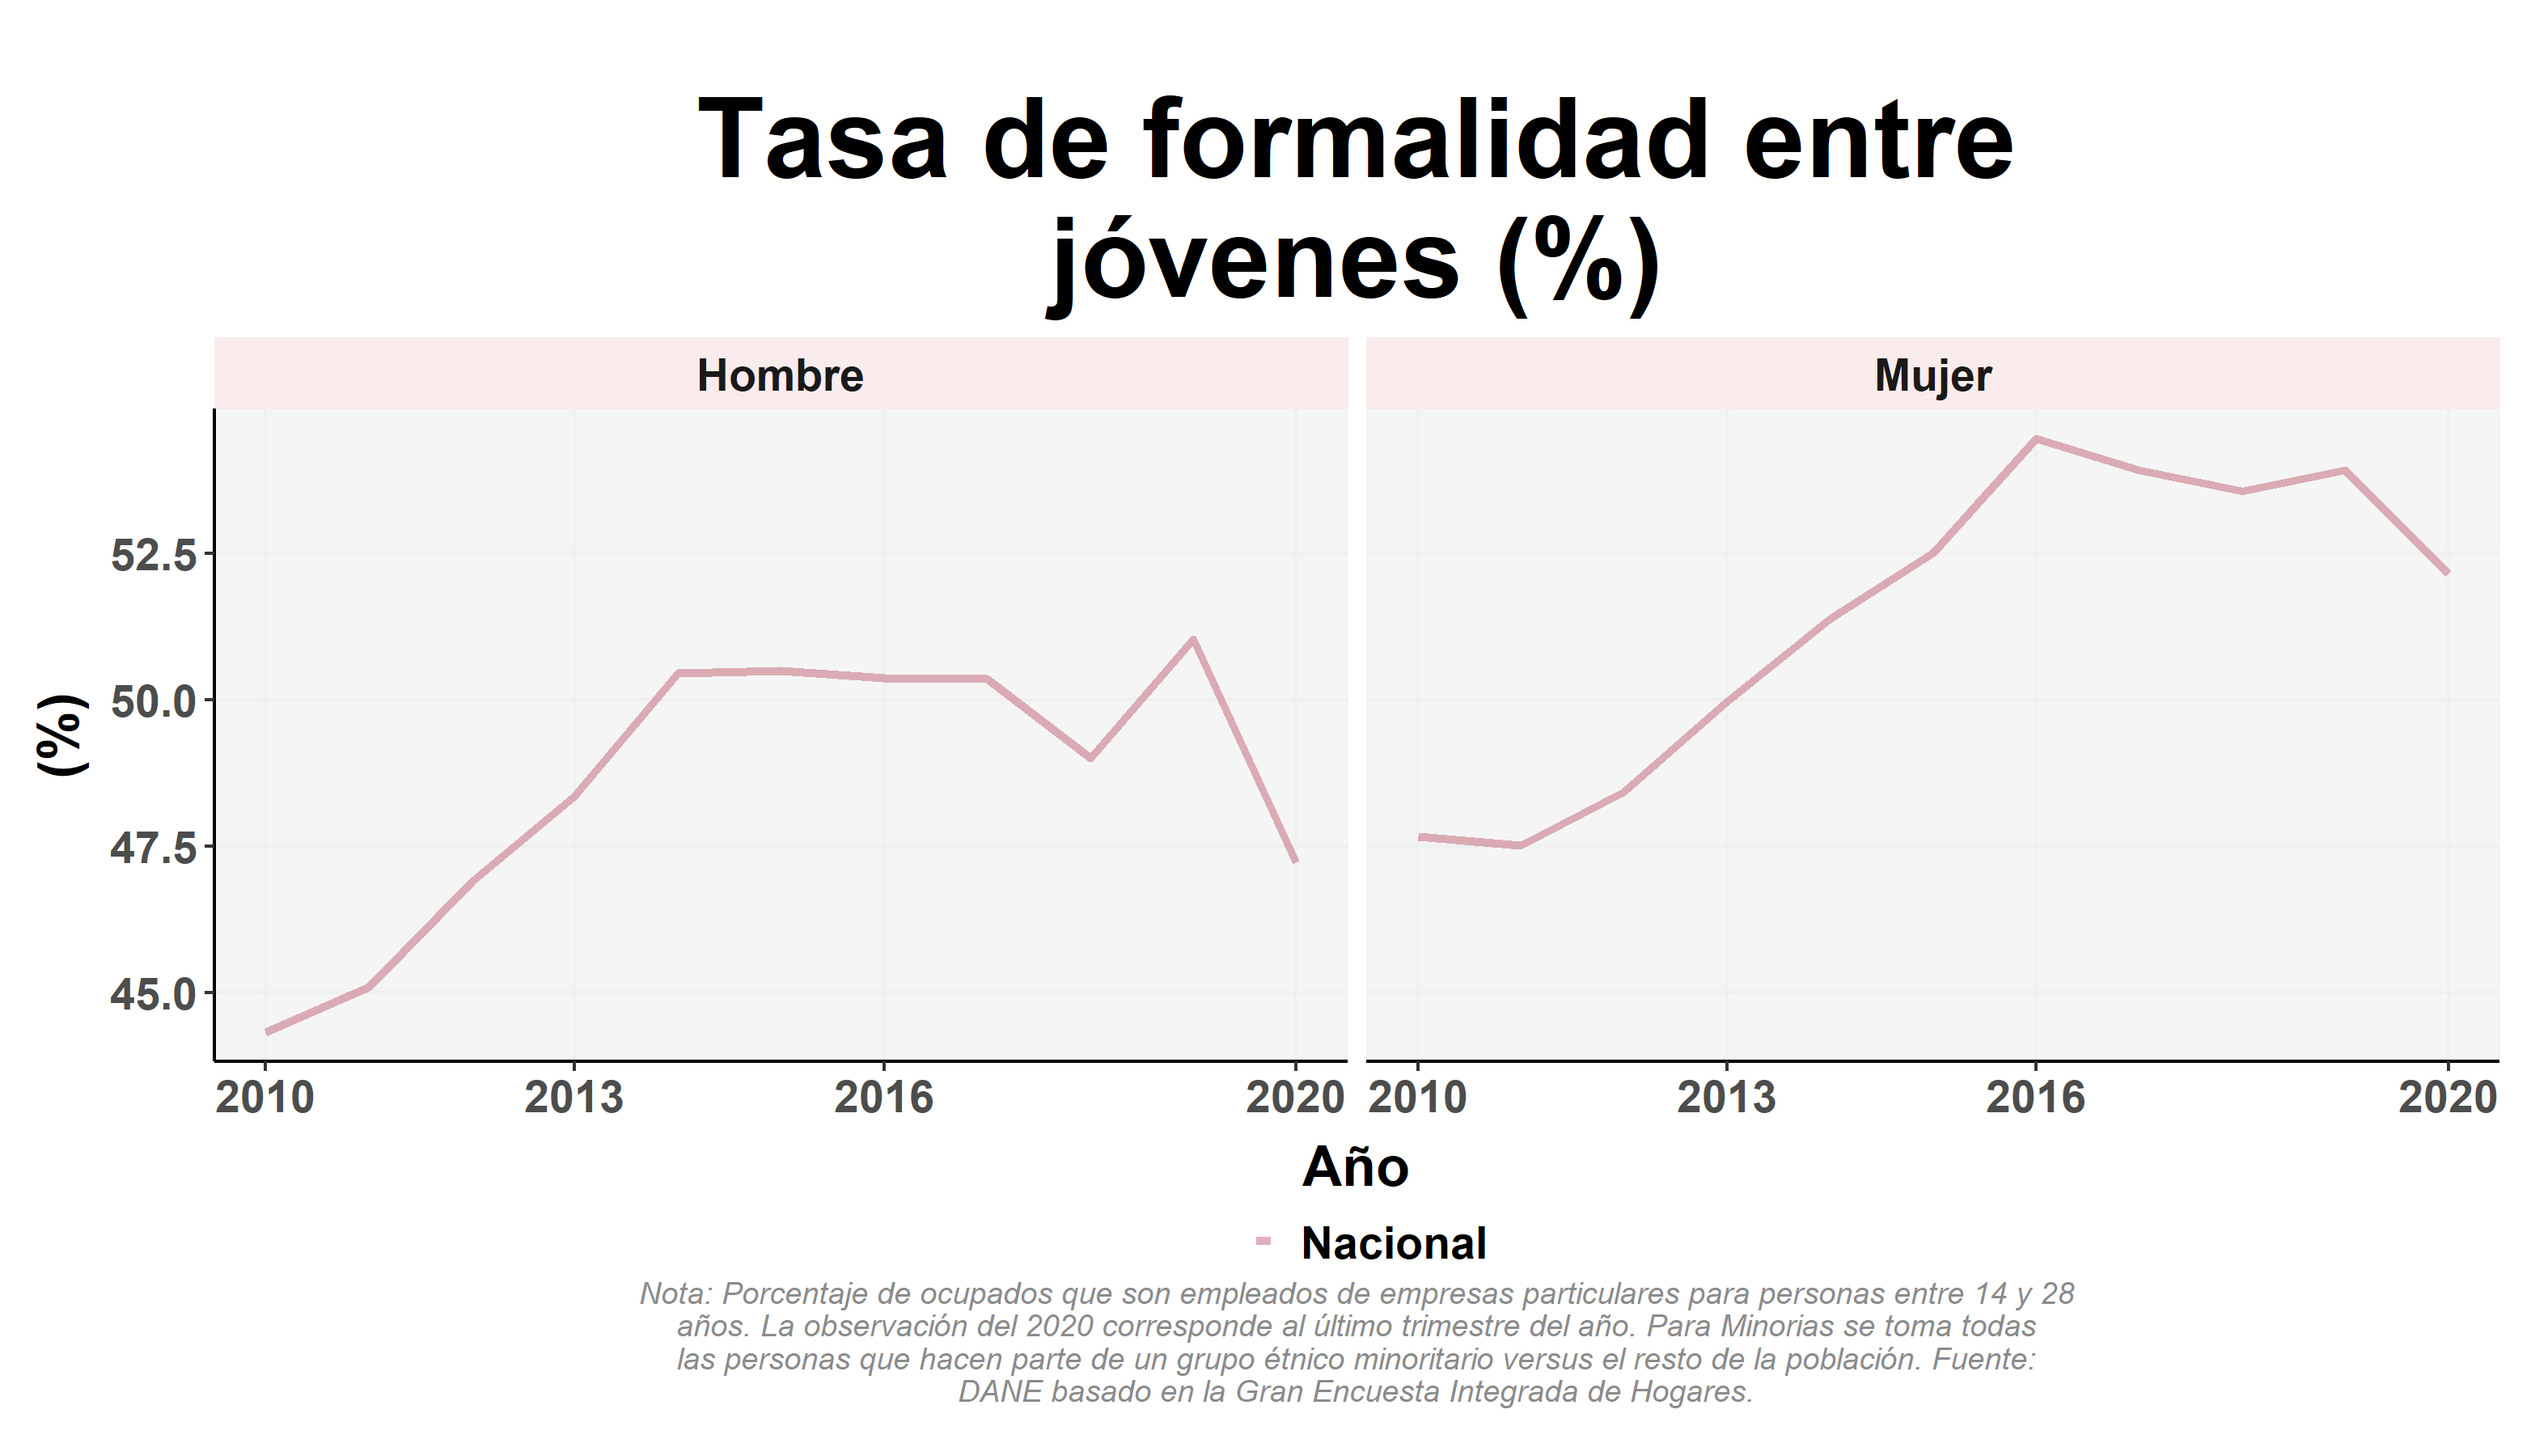
\includegraphics[width=\textwidth,keepaspectratio]{img/var_65_trend.png}
        \end{center}
    \end{figure}
            \begin{itemize}
                \item La tasa de formalidad entre géneros ha mantenido la brecha, siendo las mujeres con una tasa mayor a la de los hombres.
                \item La tasa de la mujer estuvo aumentando hasta 2016, donde se mantuvo relativamente constante hasta el 2020 donde cae a niveles cercanos a los del 2015, por otro lado la tasa para el hombre aumentó hasta el 2013, después se mantuvo constante y en 2020 decayó fuertemente, llegando a niveles cercanos del 2012.
                \item Para 2020 la tasa de formalidad masculina llegó a los niveles que tenía la de la mujer en 2010.
                \end{itemize}

%%%% Include figures
    \begin{figure}[H]
        \caption{Tasa de formalidad entre jóvenes por minorías y no minorías para 2020 \label{map_result_2} }
        \begin{center}
        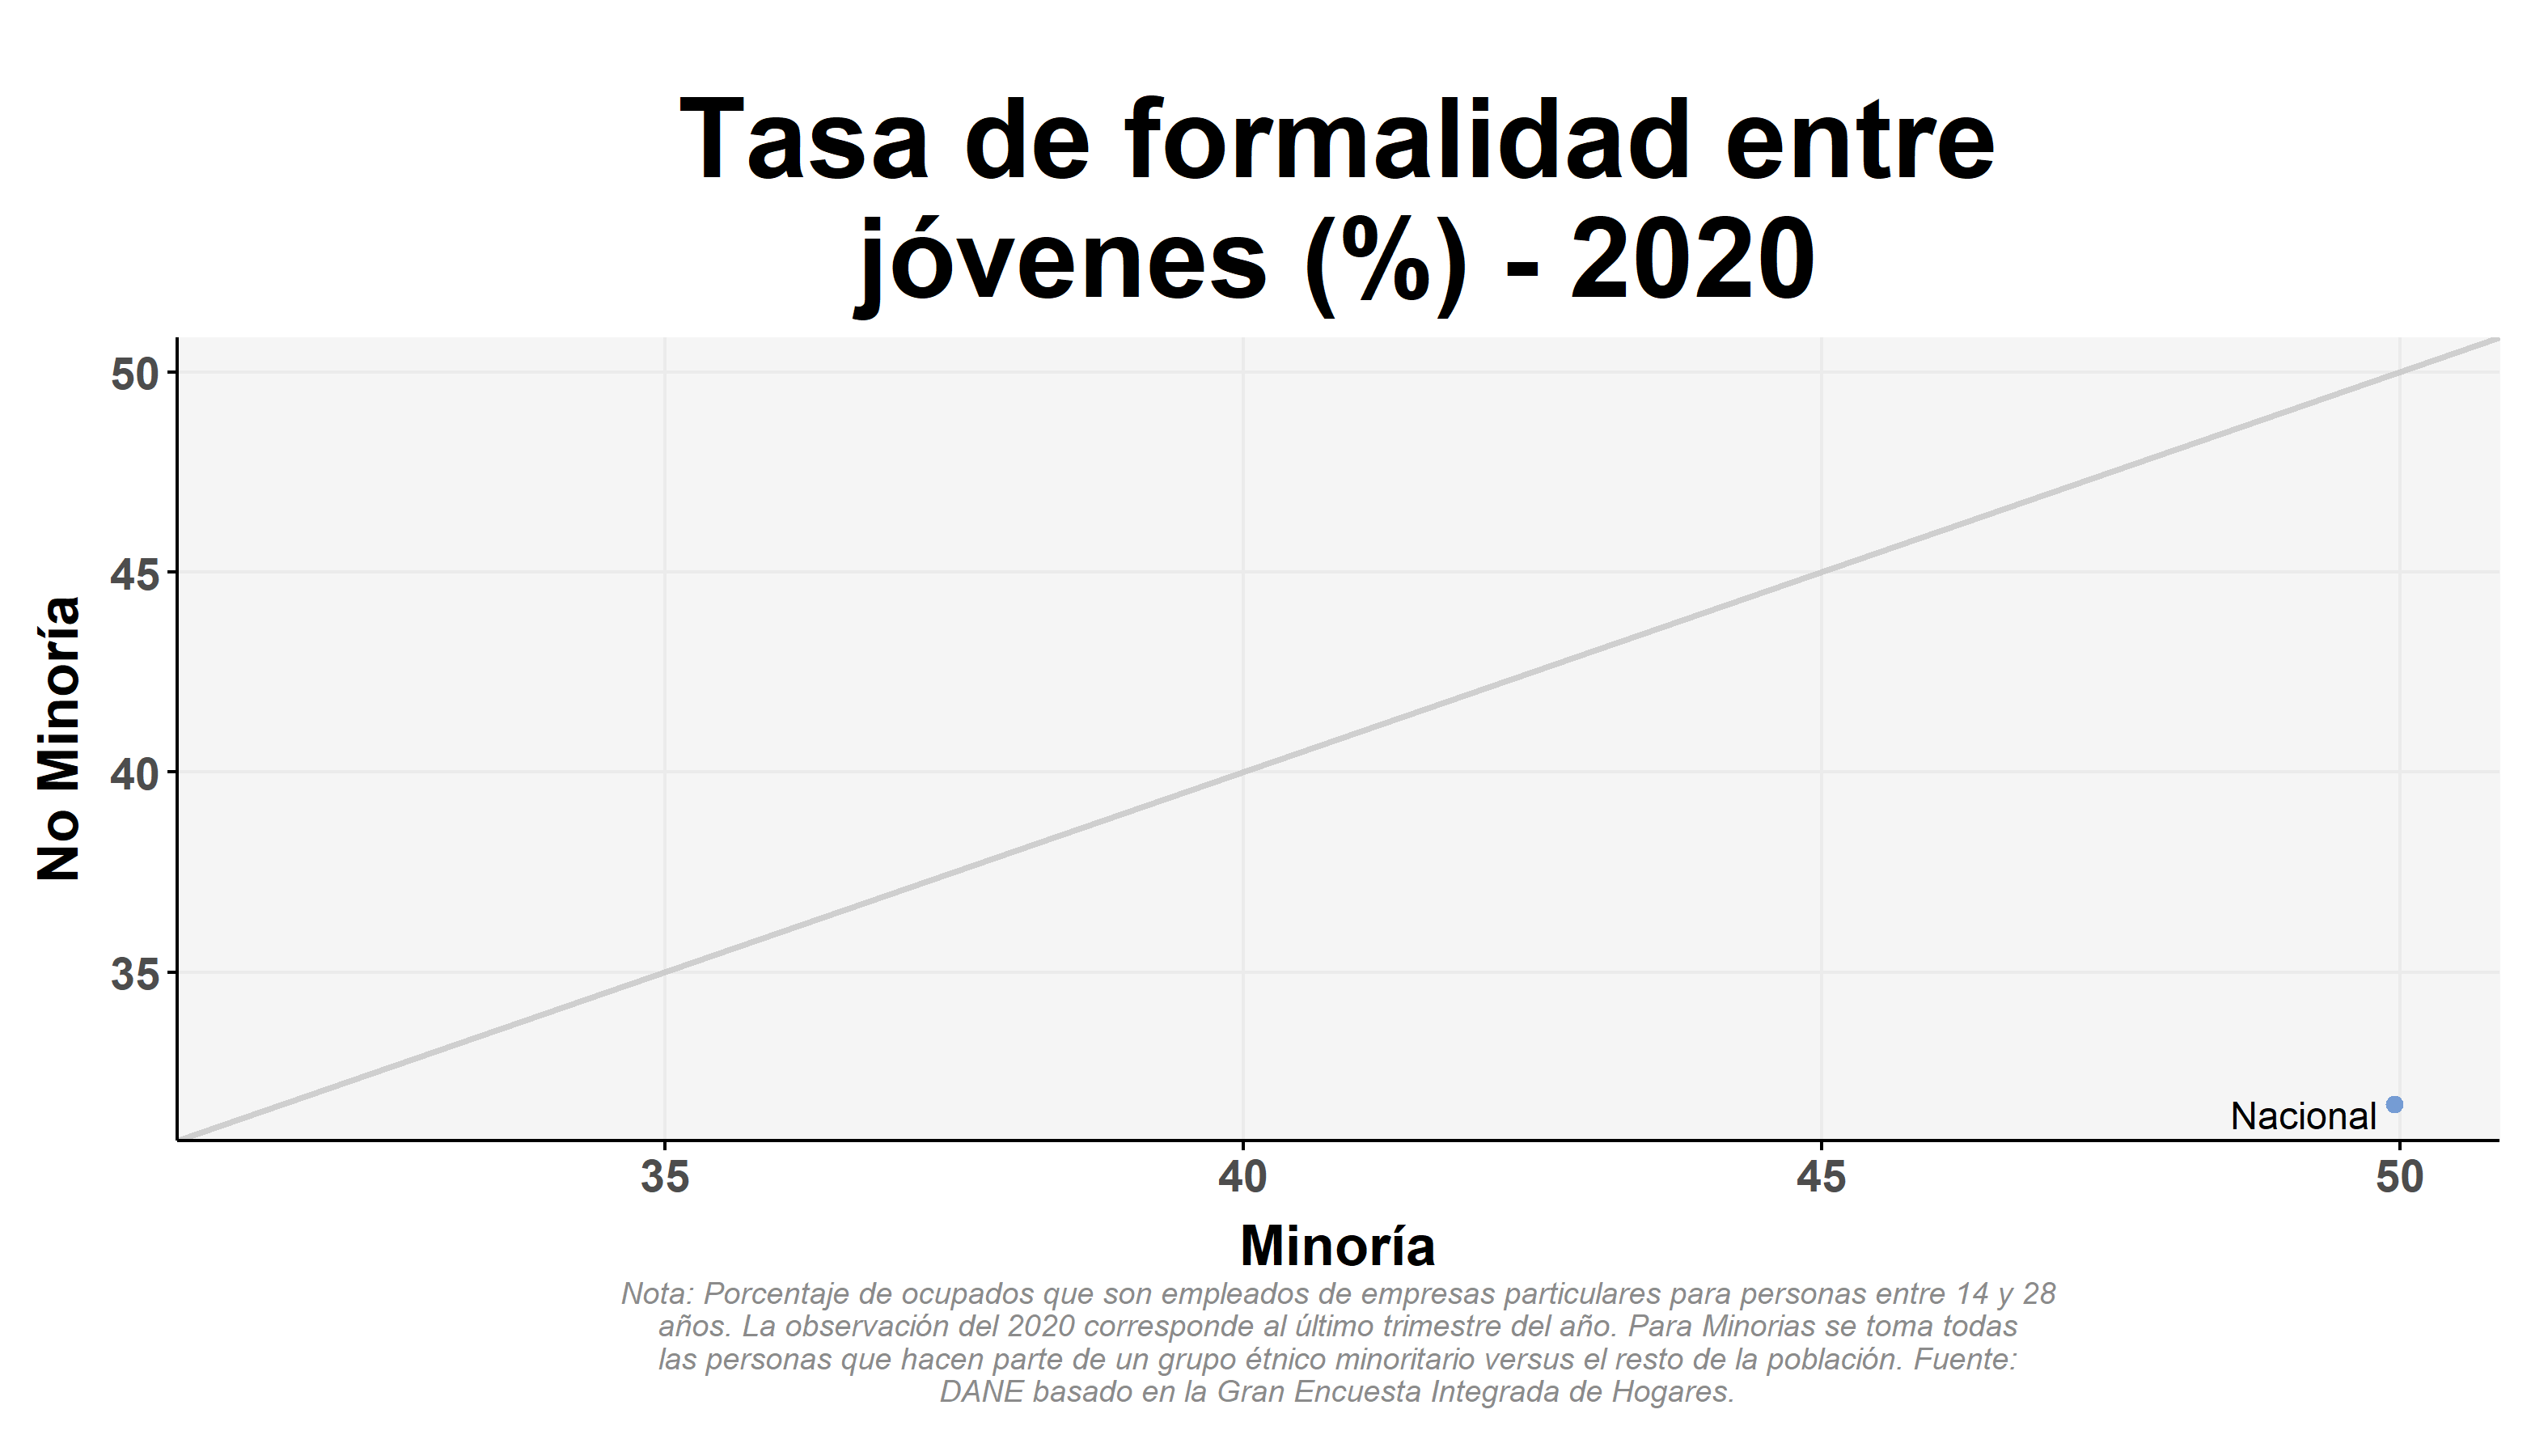
\includegraphics[width=\textwidth,keepaspectratio]{img/var_64_scatter.png}
        \end{center}
    \end{figure}
            \begin{itemize}
                \item Las minorías tienen una mayor tasa de formalidad con un 50\%, mientras que las no minorías es de poco más del 30\%.
                \end{itemize}

    \subsection{Empleo informal}

%%%% Include figures
    \begin{figure}[H]
        \caption{Tasa de informalidad entre jóvenes a nivel nacional \label{map_result_2} }
        \begin{center}
        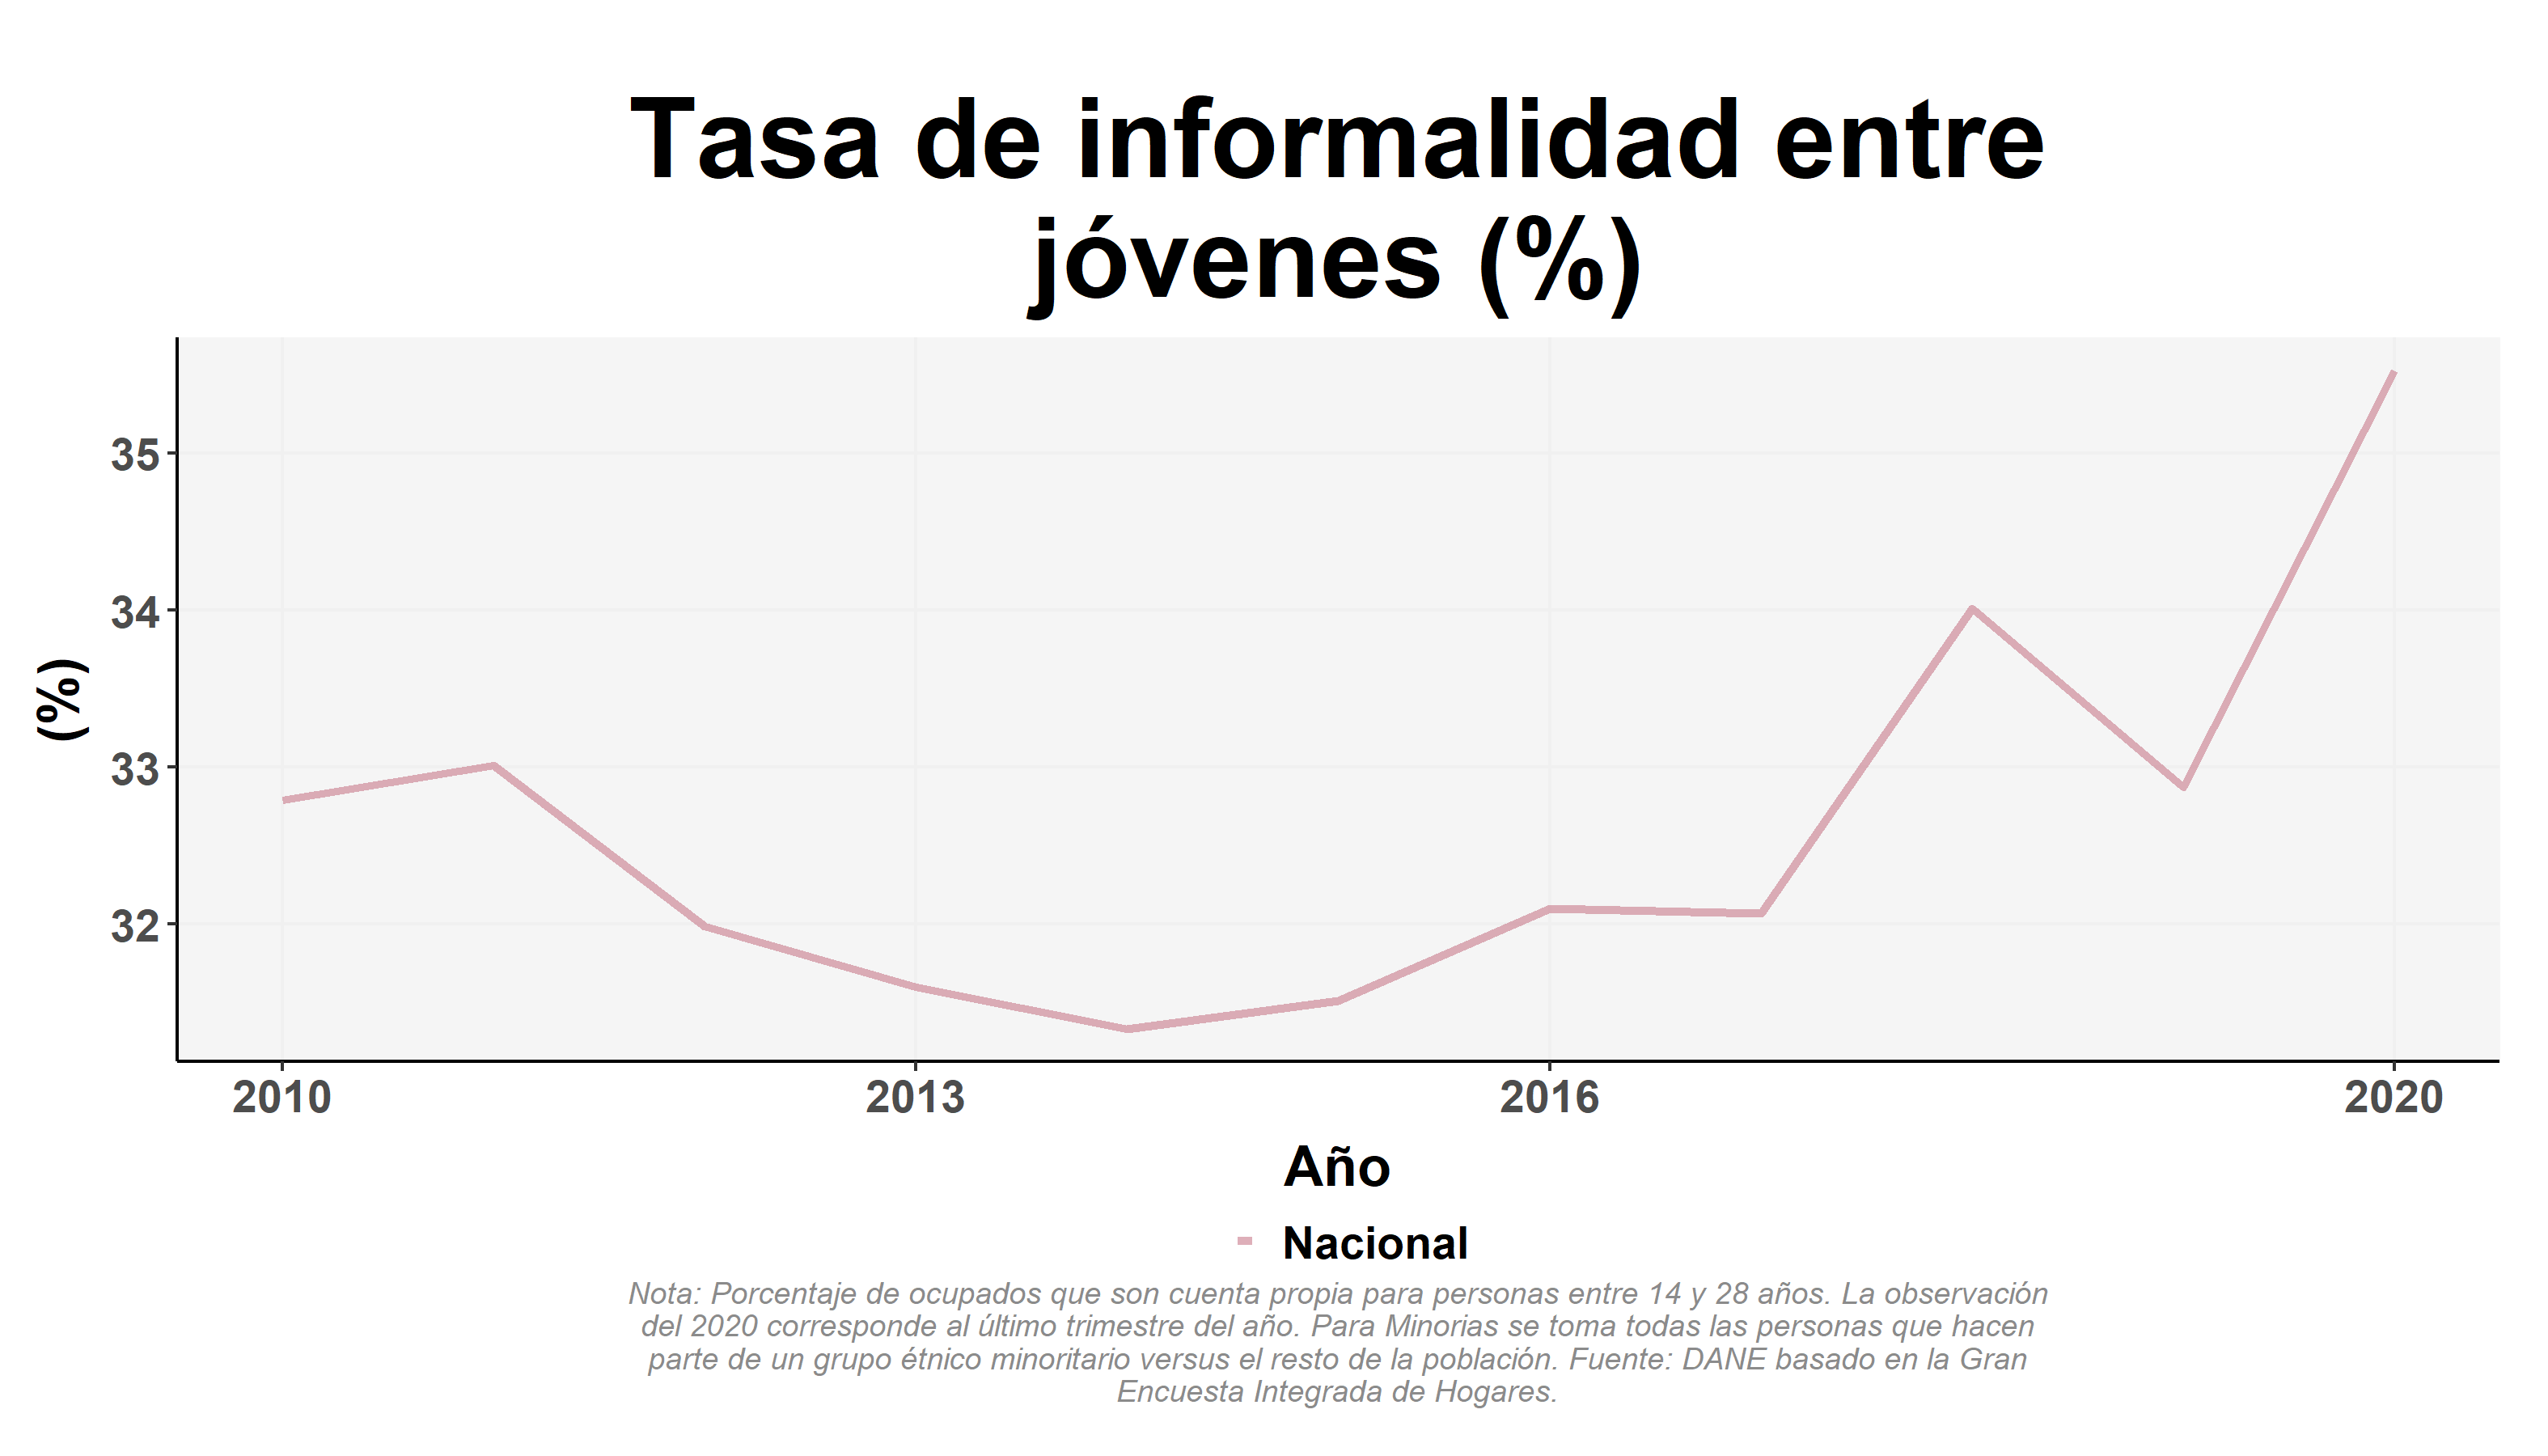
\includegraphics[width=\textwidth,keepaspectratio]{img/var_76_trend.png}
        \end{center}
    \end{figure}
            \begin{itemize}
                \item En la primera mitad de la década la tasa de informalidad para jóvenes estaba disminuyendo, pero desde el 2018 ha aumentado significativamente, superando los niveles registrado para el 2010, en especial para 2020.
                \item El 2020 registró un aumento significativo dada la emergencia sanitaria.
                \end{itemize}

%%%% Include figures
    \begin{figure}[H]
        \caption{Tasa de informalidad entre jóvenes por género \label{map_result_2} }
        \begin{center}
        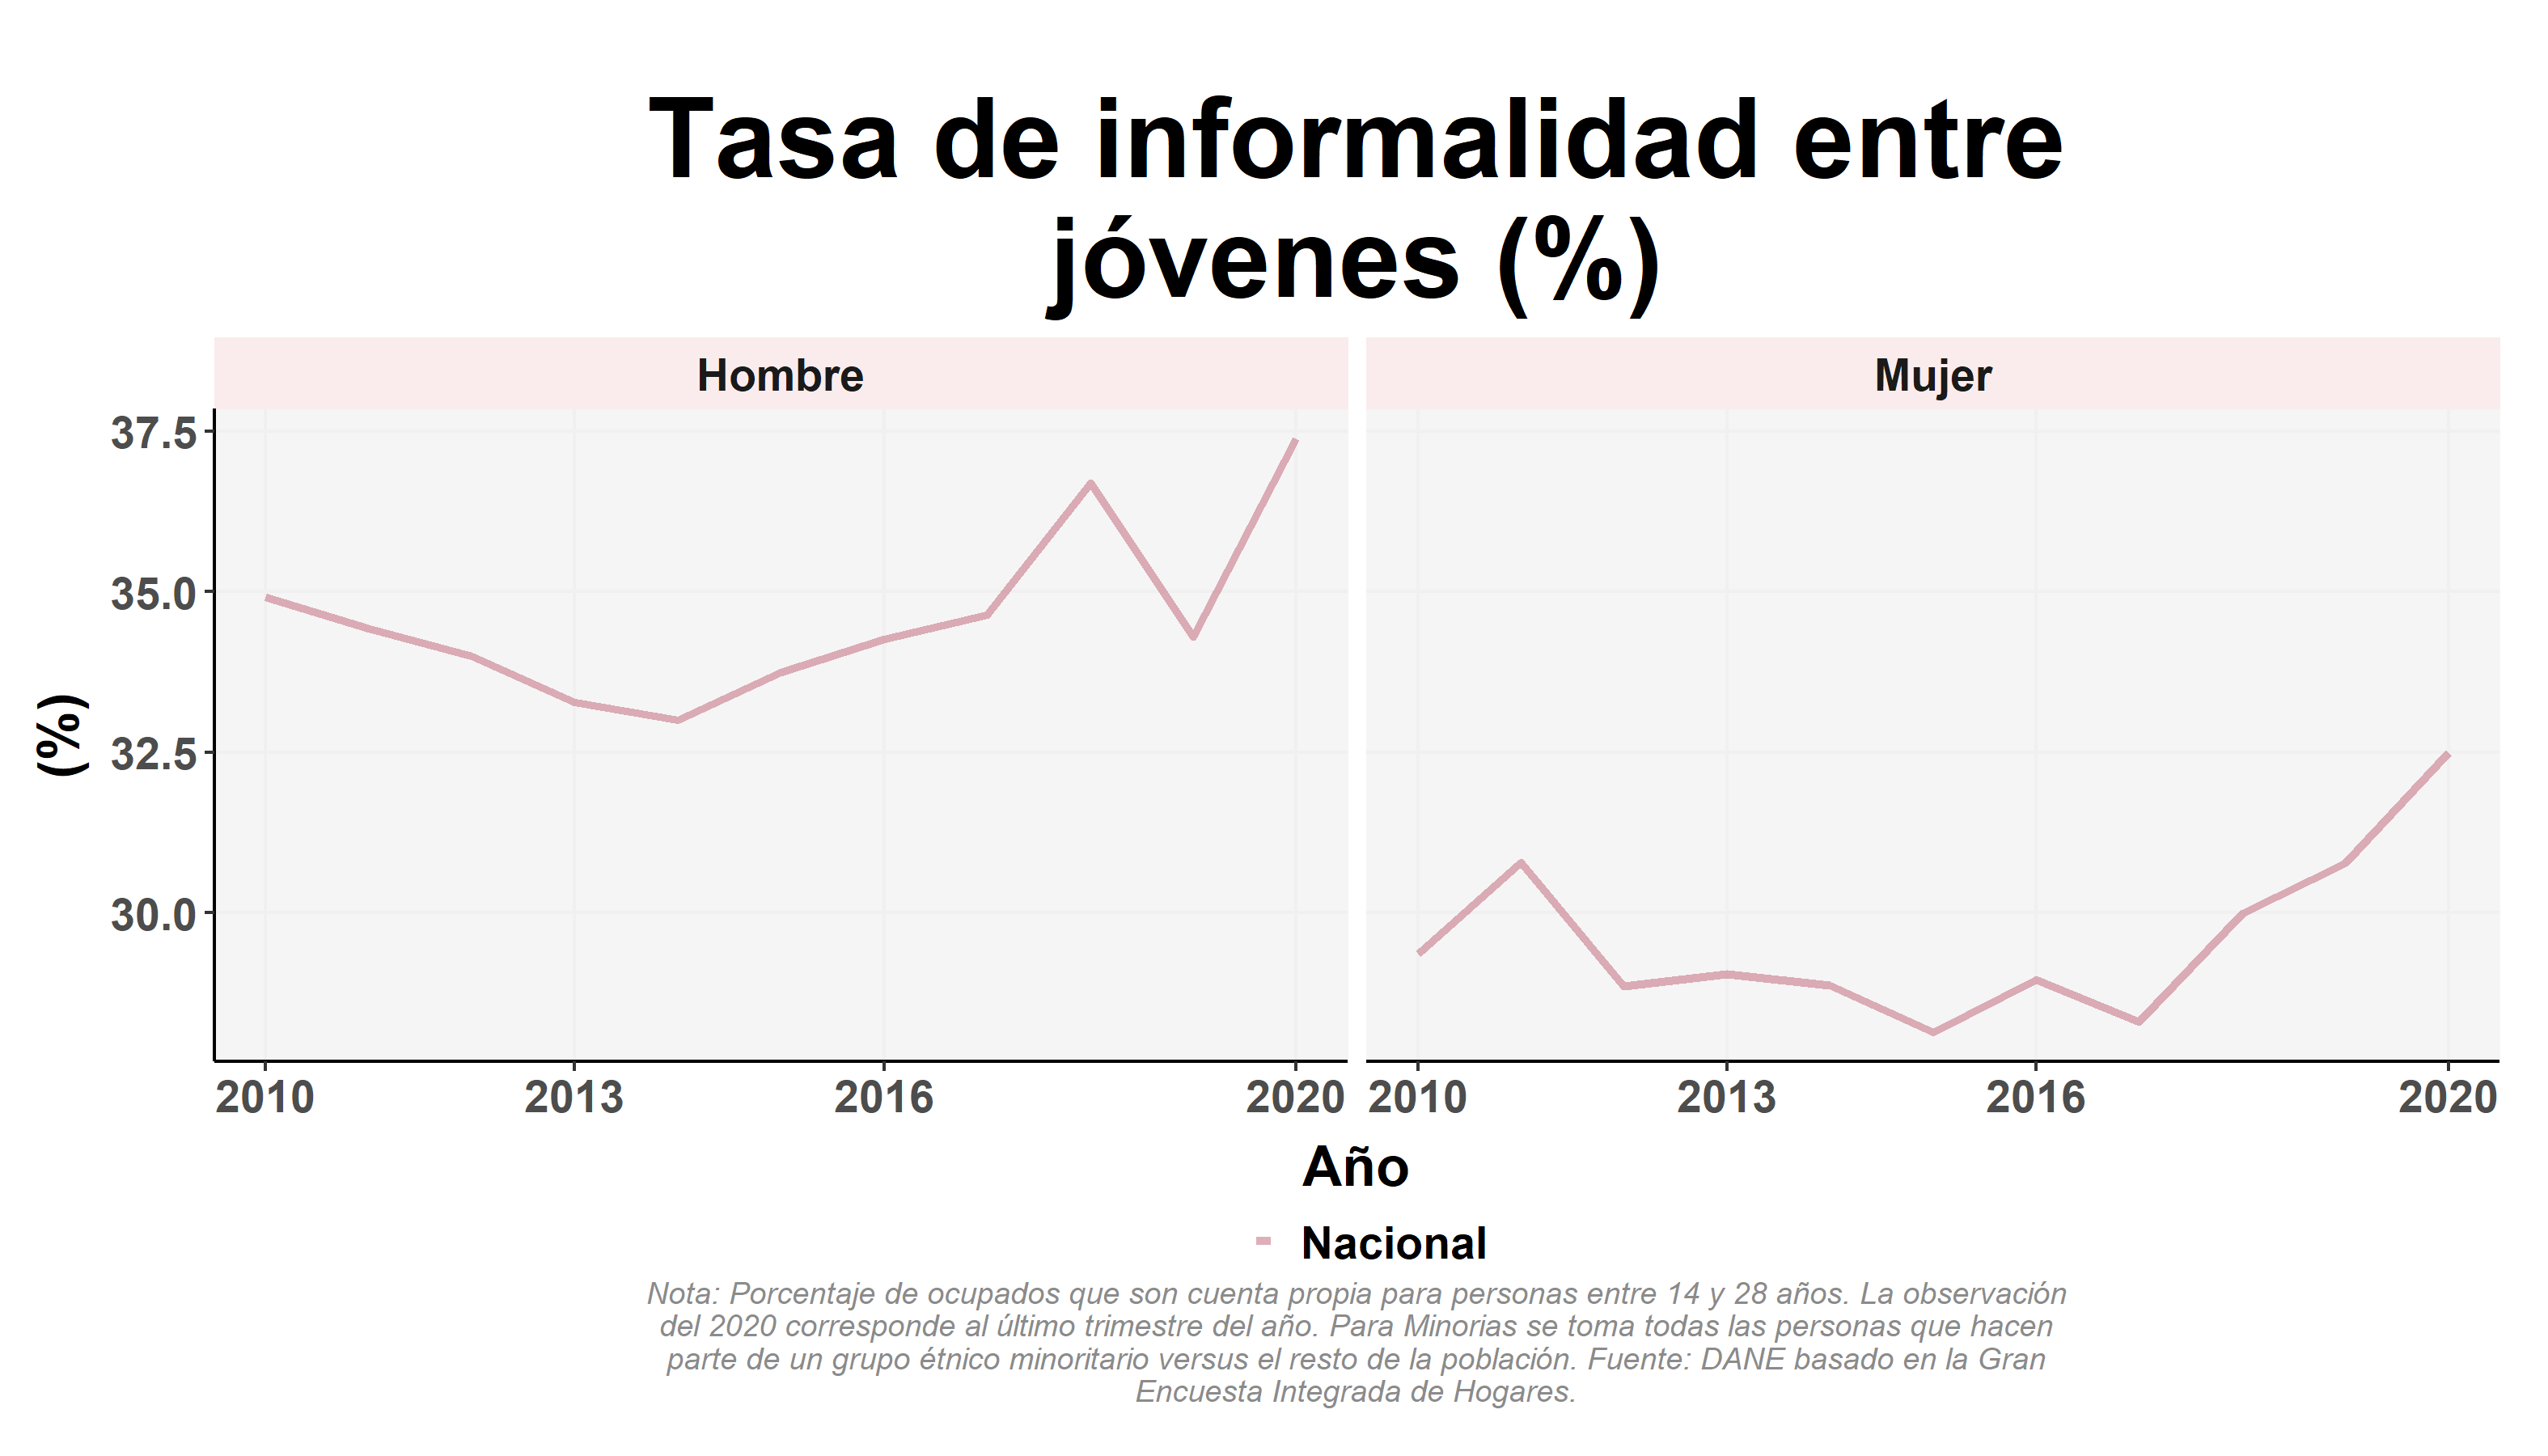
\includegraphics[width=\textwidth,keepaspectratio]{img/var_75_trend.png}
        \end{center}
    \end{figure}
            \begin{itemize}
                \item La brecha entre hombre y mujeres se ha mantenido, siendo la tasa de informalidad del hombre más alta a la de la mujer.
                \item Desde 2014 ambas tasas de informalidad del hombre ha estado aumentando, mientras que la de la mujer se mantuvo casi estable hasta 2017 donde inició a aumentar de manera constante.
                \end{itemize}

%%%% Include figures
    \begin{figure}[H]
        \caption{Tasa de informalidad entre jóvenes por minorías y no minorías para 2020 \label{map_result_2} }
        \begin{center}
        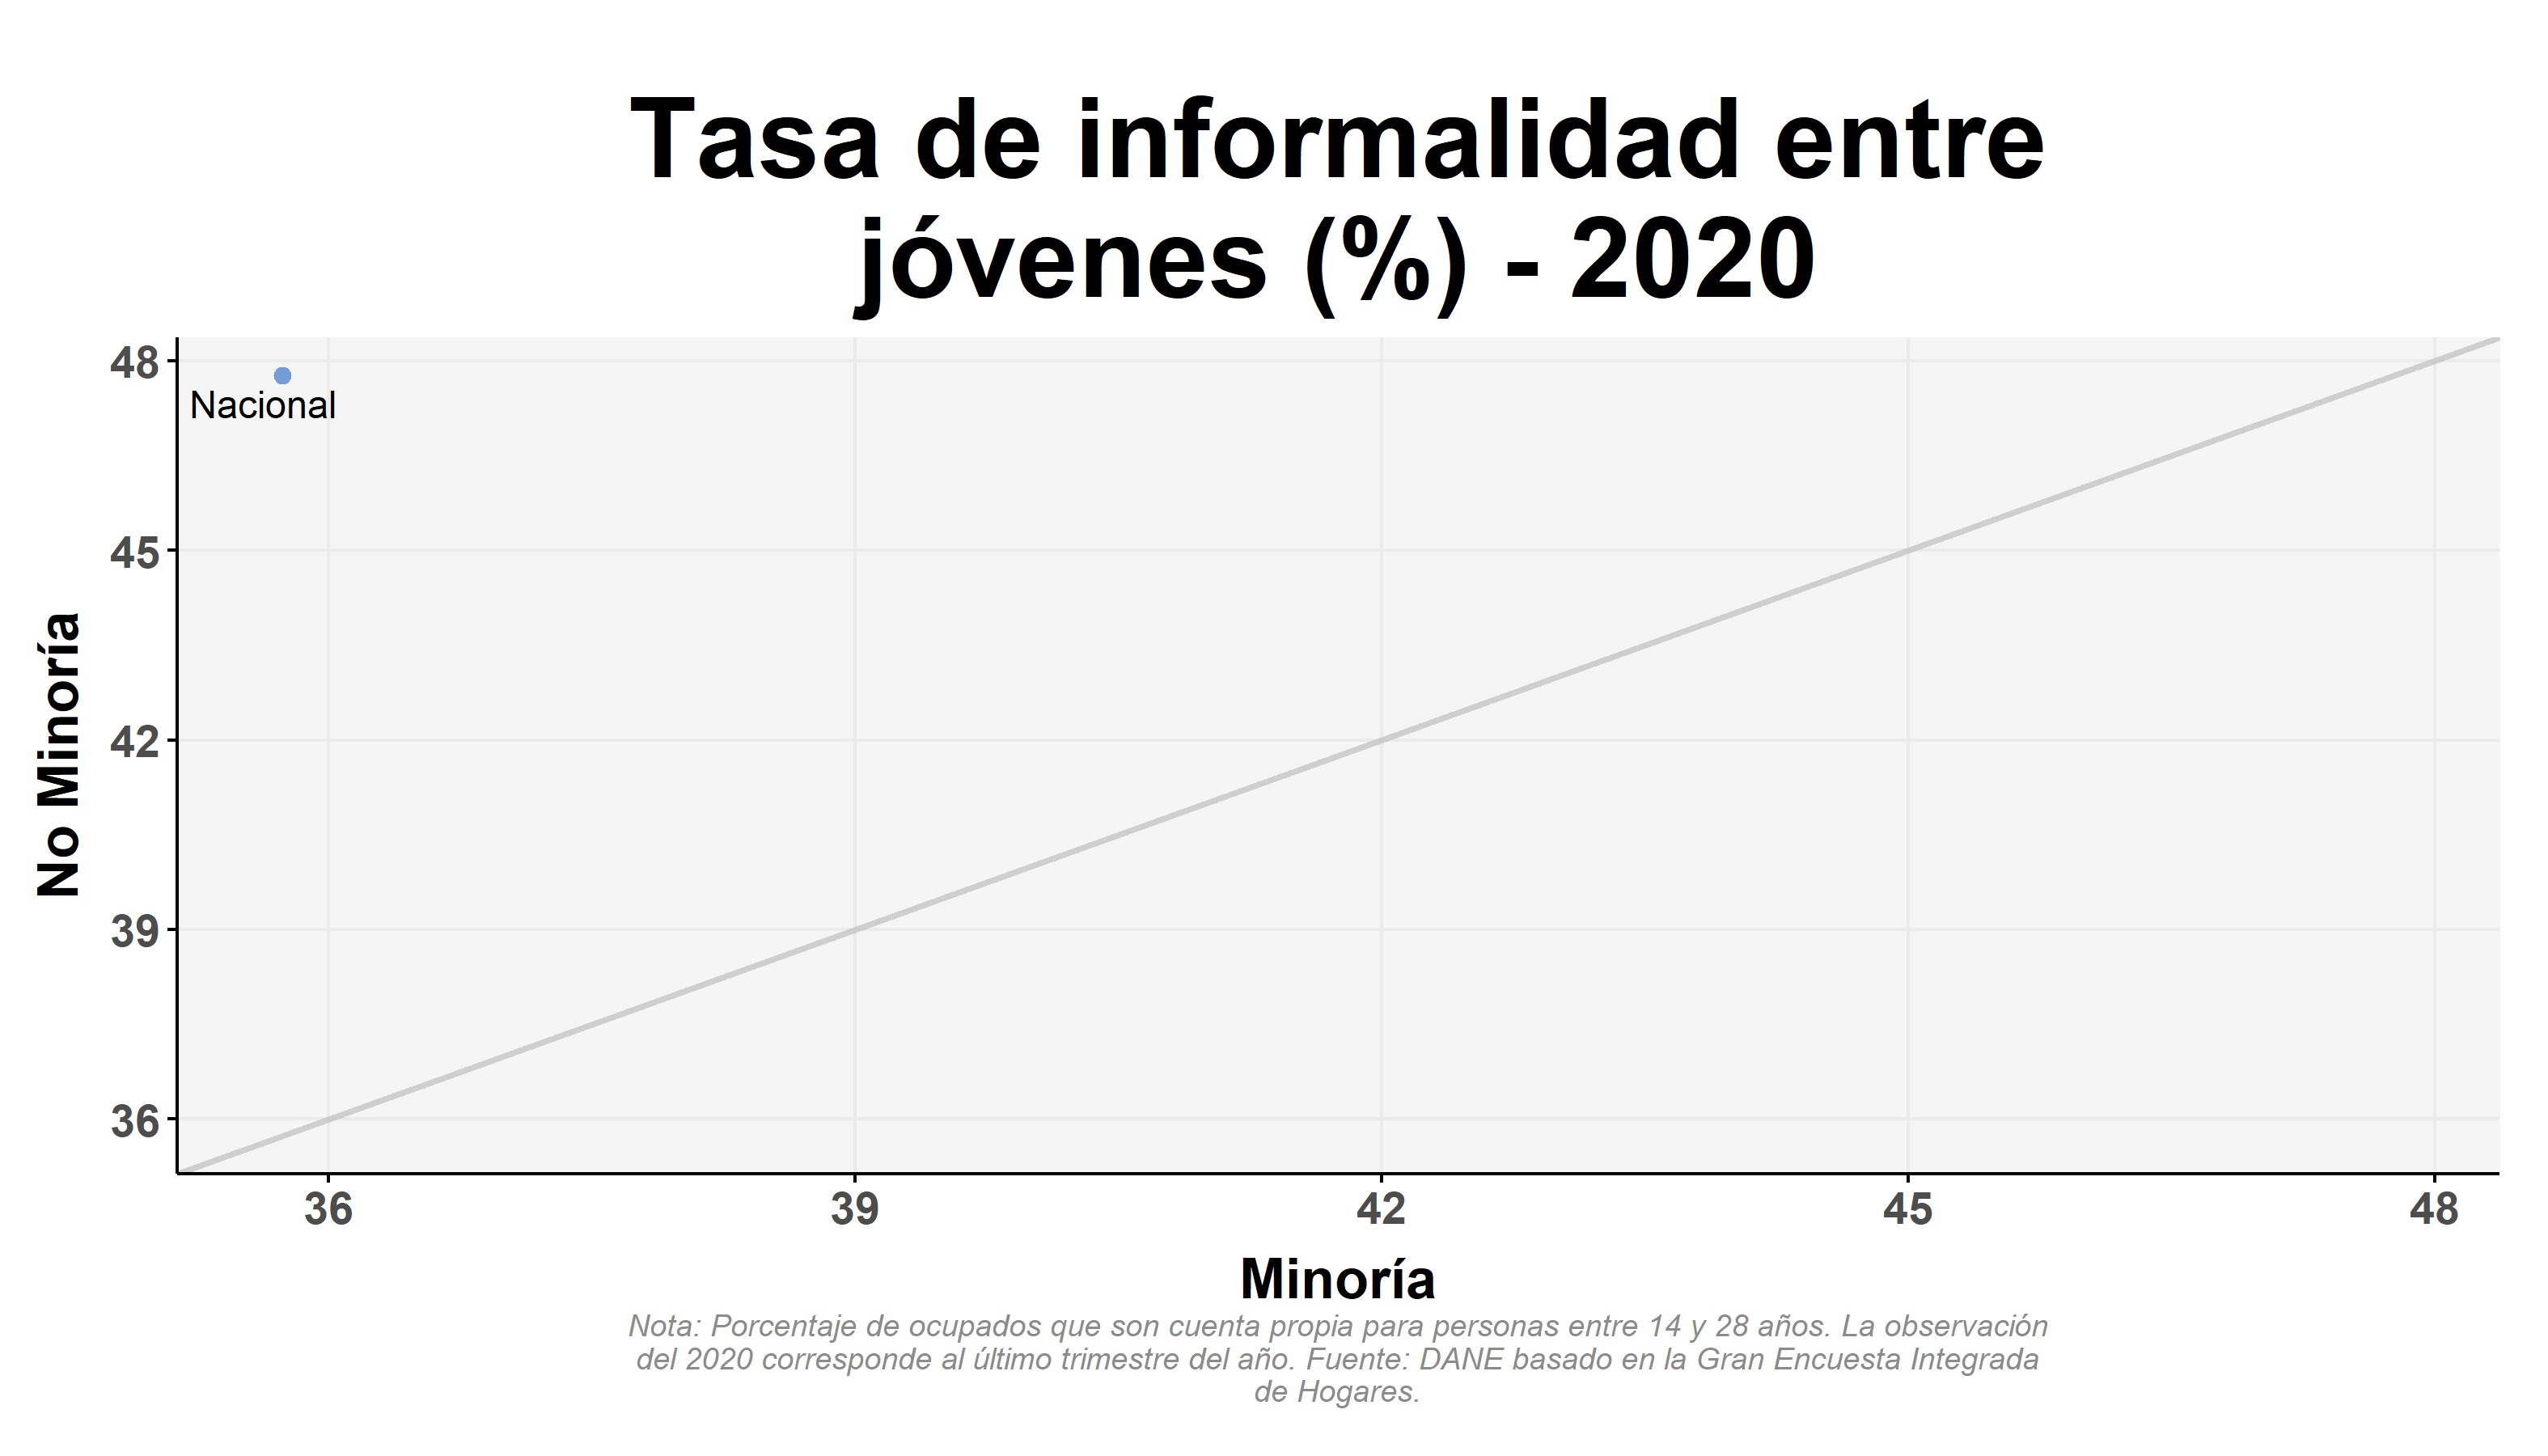
\includegraphics[width=\textwidth,keepaspectratio]{img/var_74_scatter.png}
        \end{center}
    \end{figure}
            \begin{itemize}
                \item La tasa de informalidad es mayor para las no minorías que las minorías con una diferencia aproximada del 12\%.
                \end{itemize}

    \subsection{Ingreso laboral}

%%%% Include figures
    \begin{figure}[H]
        \caption{Percentil 25 del ingreso laboral de los jóvenes a nivel nacional \label{map_result_2} }
        \begin{center}
        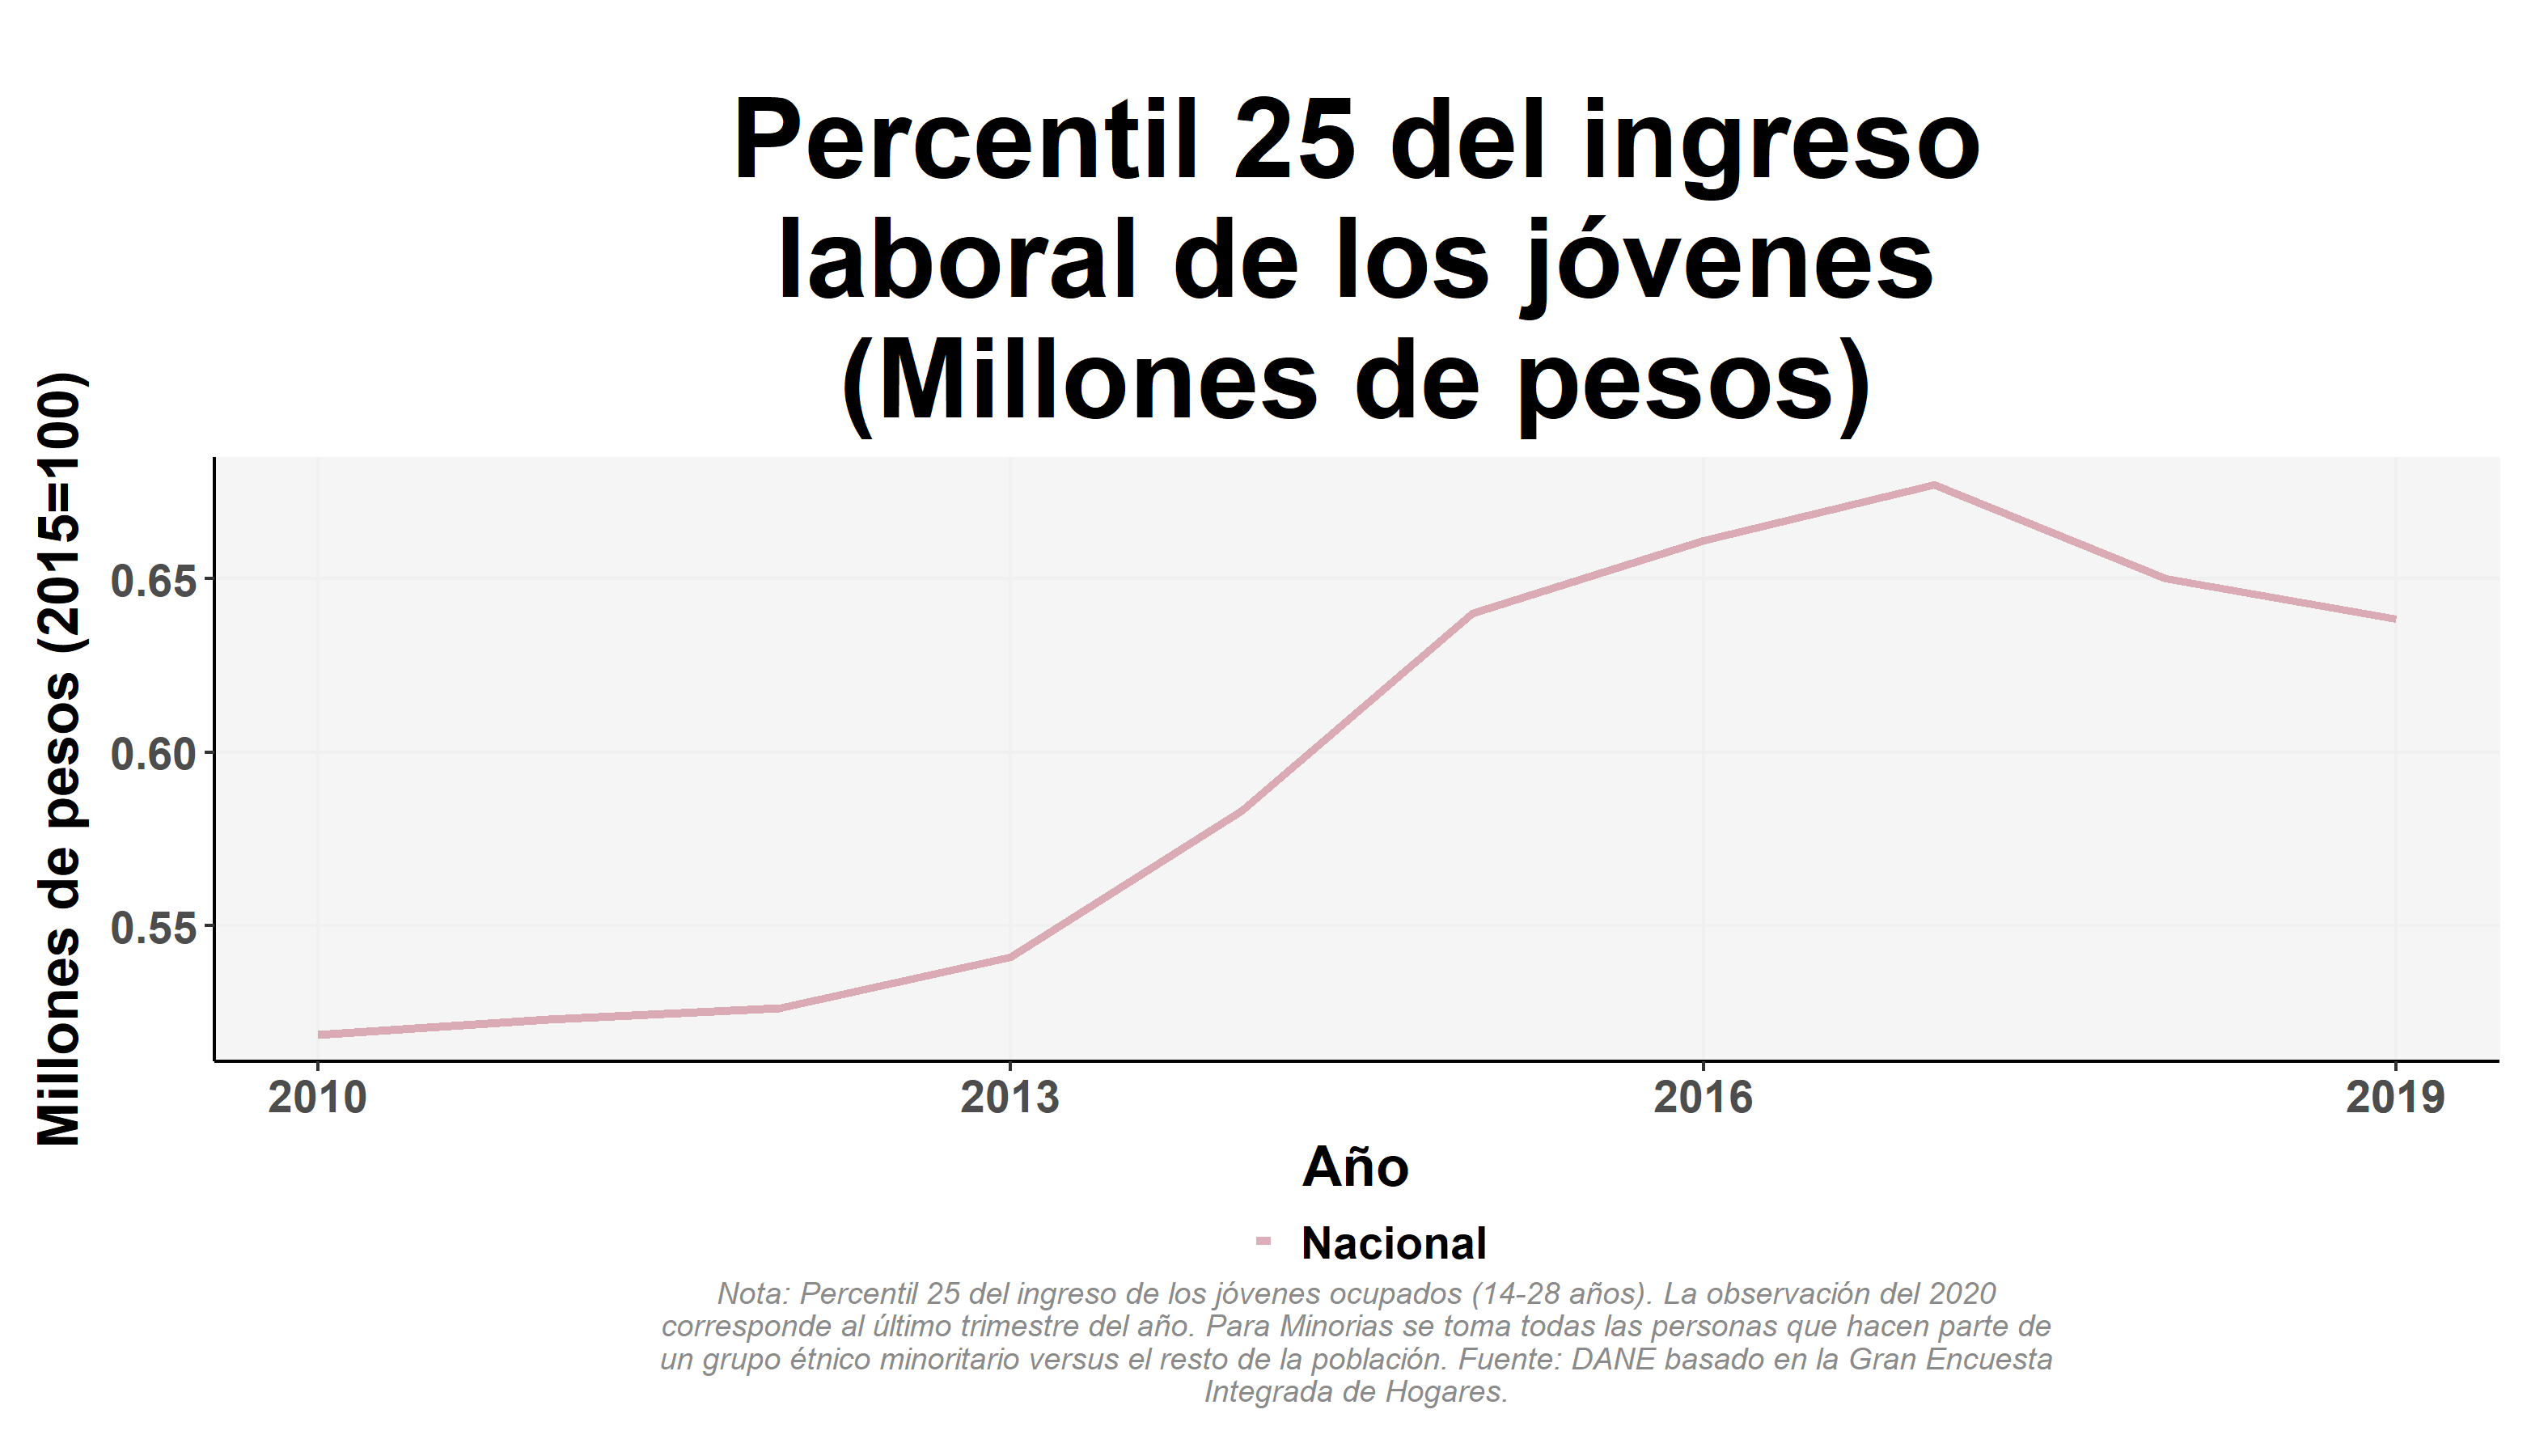
\includegraphics[width=\textwidth,keepaspectratio]{img/var_13_trend.png}
        \end{center}
    \end{figure}
            \begin{itemize}
                \item Hasta 2017 estuvo aumentando el ingreso laboral para el percentil 25, después de eso ha estado disminuyendo.
                \end{itemize}

%%%% Include figures
    \begin{figure}[H]
        \caption{Percentil 25 del ingreso laboral de los jóvenes por género \label{map_result_2} }
        \begin{center}
        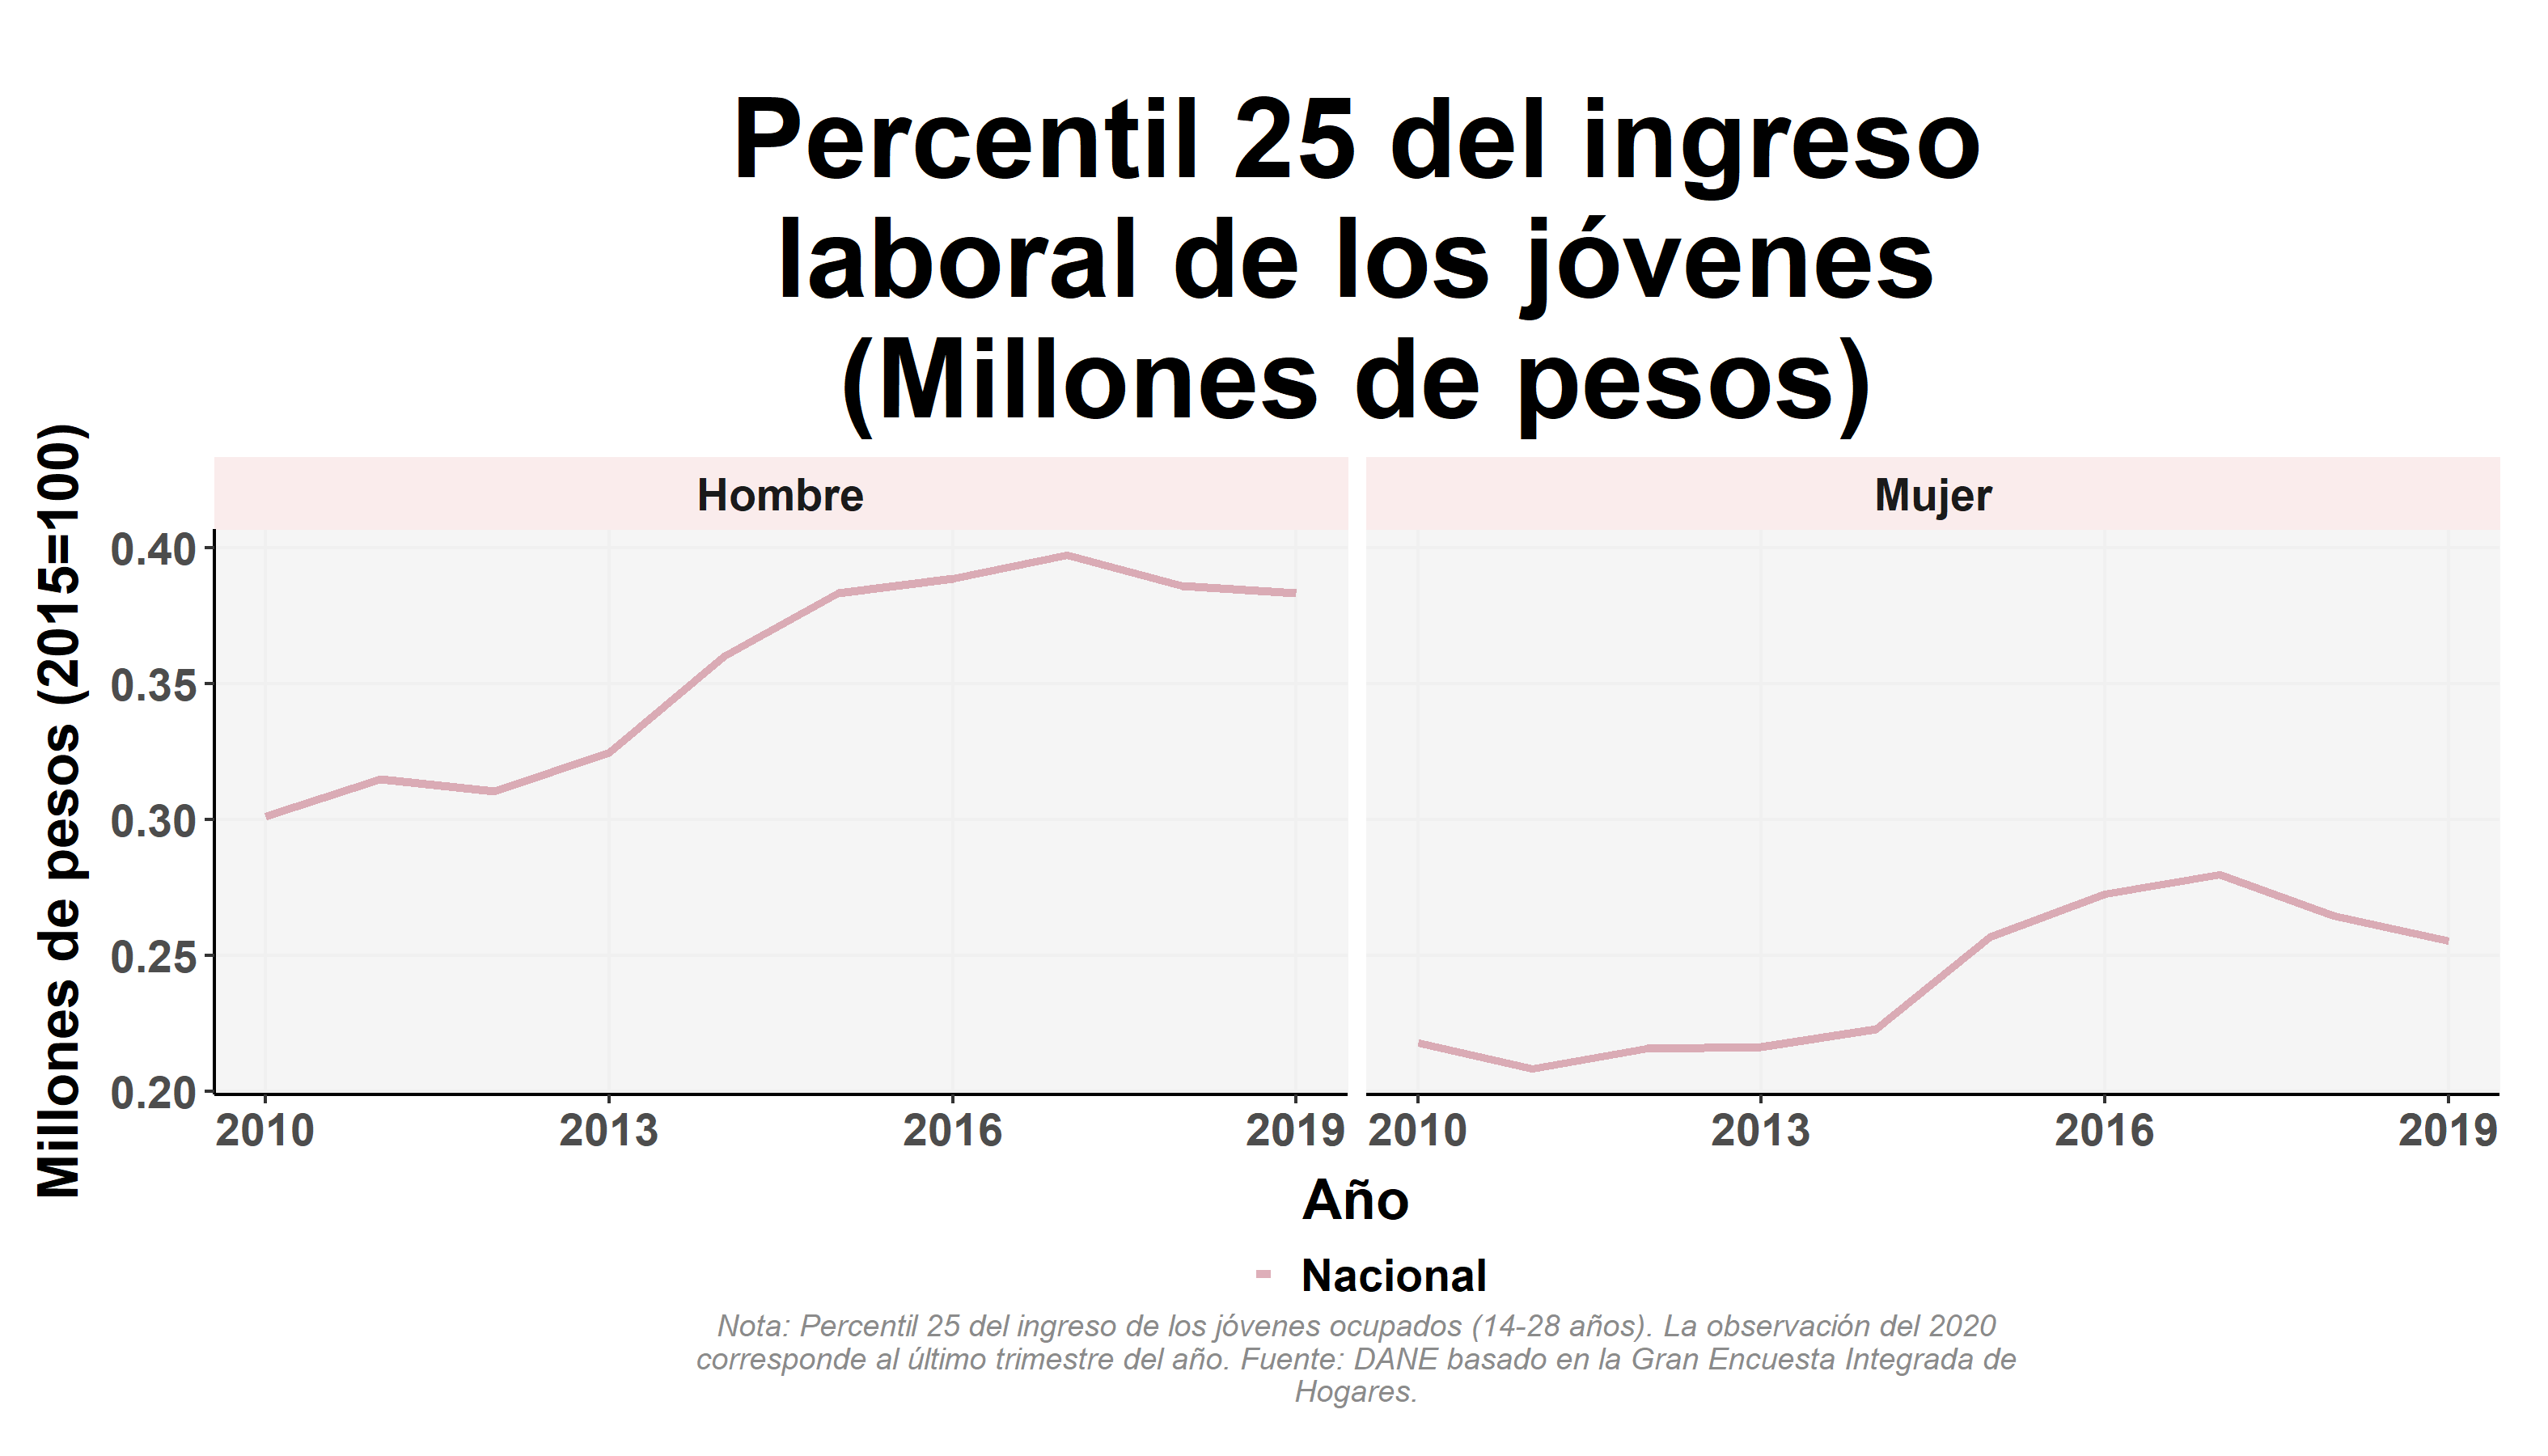
\includegraphics[width=\textwidth,keepaspectratio]{img/var_12_trend.png}
        \end{center}
    \end{figure}
            \begin{itemize}
                \item La brecha de ingresos de género entre jóvenes para el percentil 25 se ha mantenido en los años, siendo el ingreso de las mujeres menor.
                \item Hasta el 2017 los ingresos laborales estaban aumentando, después inició a disminuir retrocediendo a los valores de 2015 para ambos.
                \end{itemize}

%%%% Include figures
    \begin{figure}[H]
        \caption{Percentil 25 del ingreso laboral de los jóvenes por minorías y no minorías para 2020 \label{map_result_2} }
        \begin{center}
        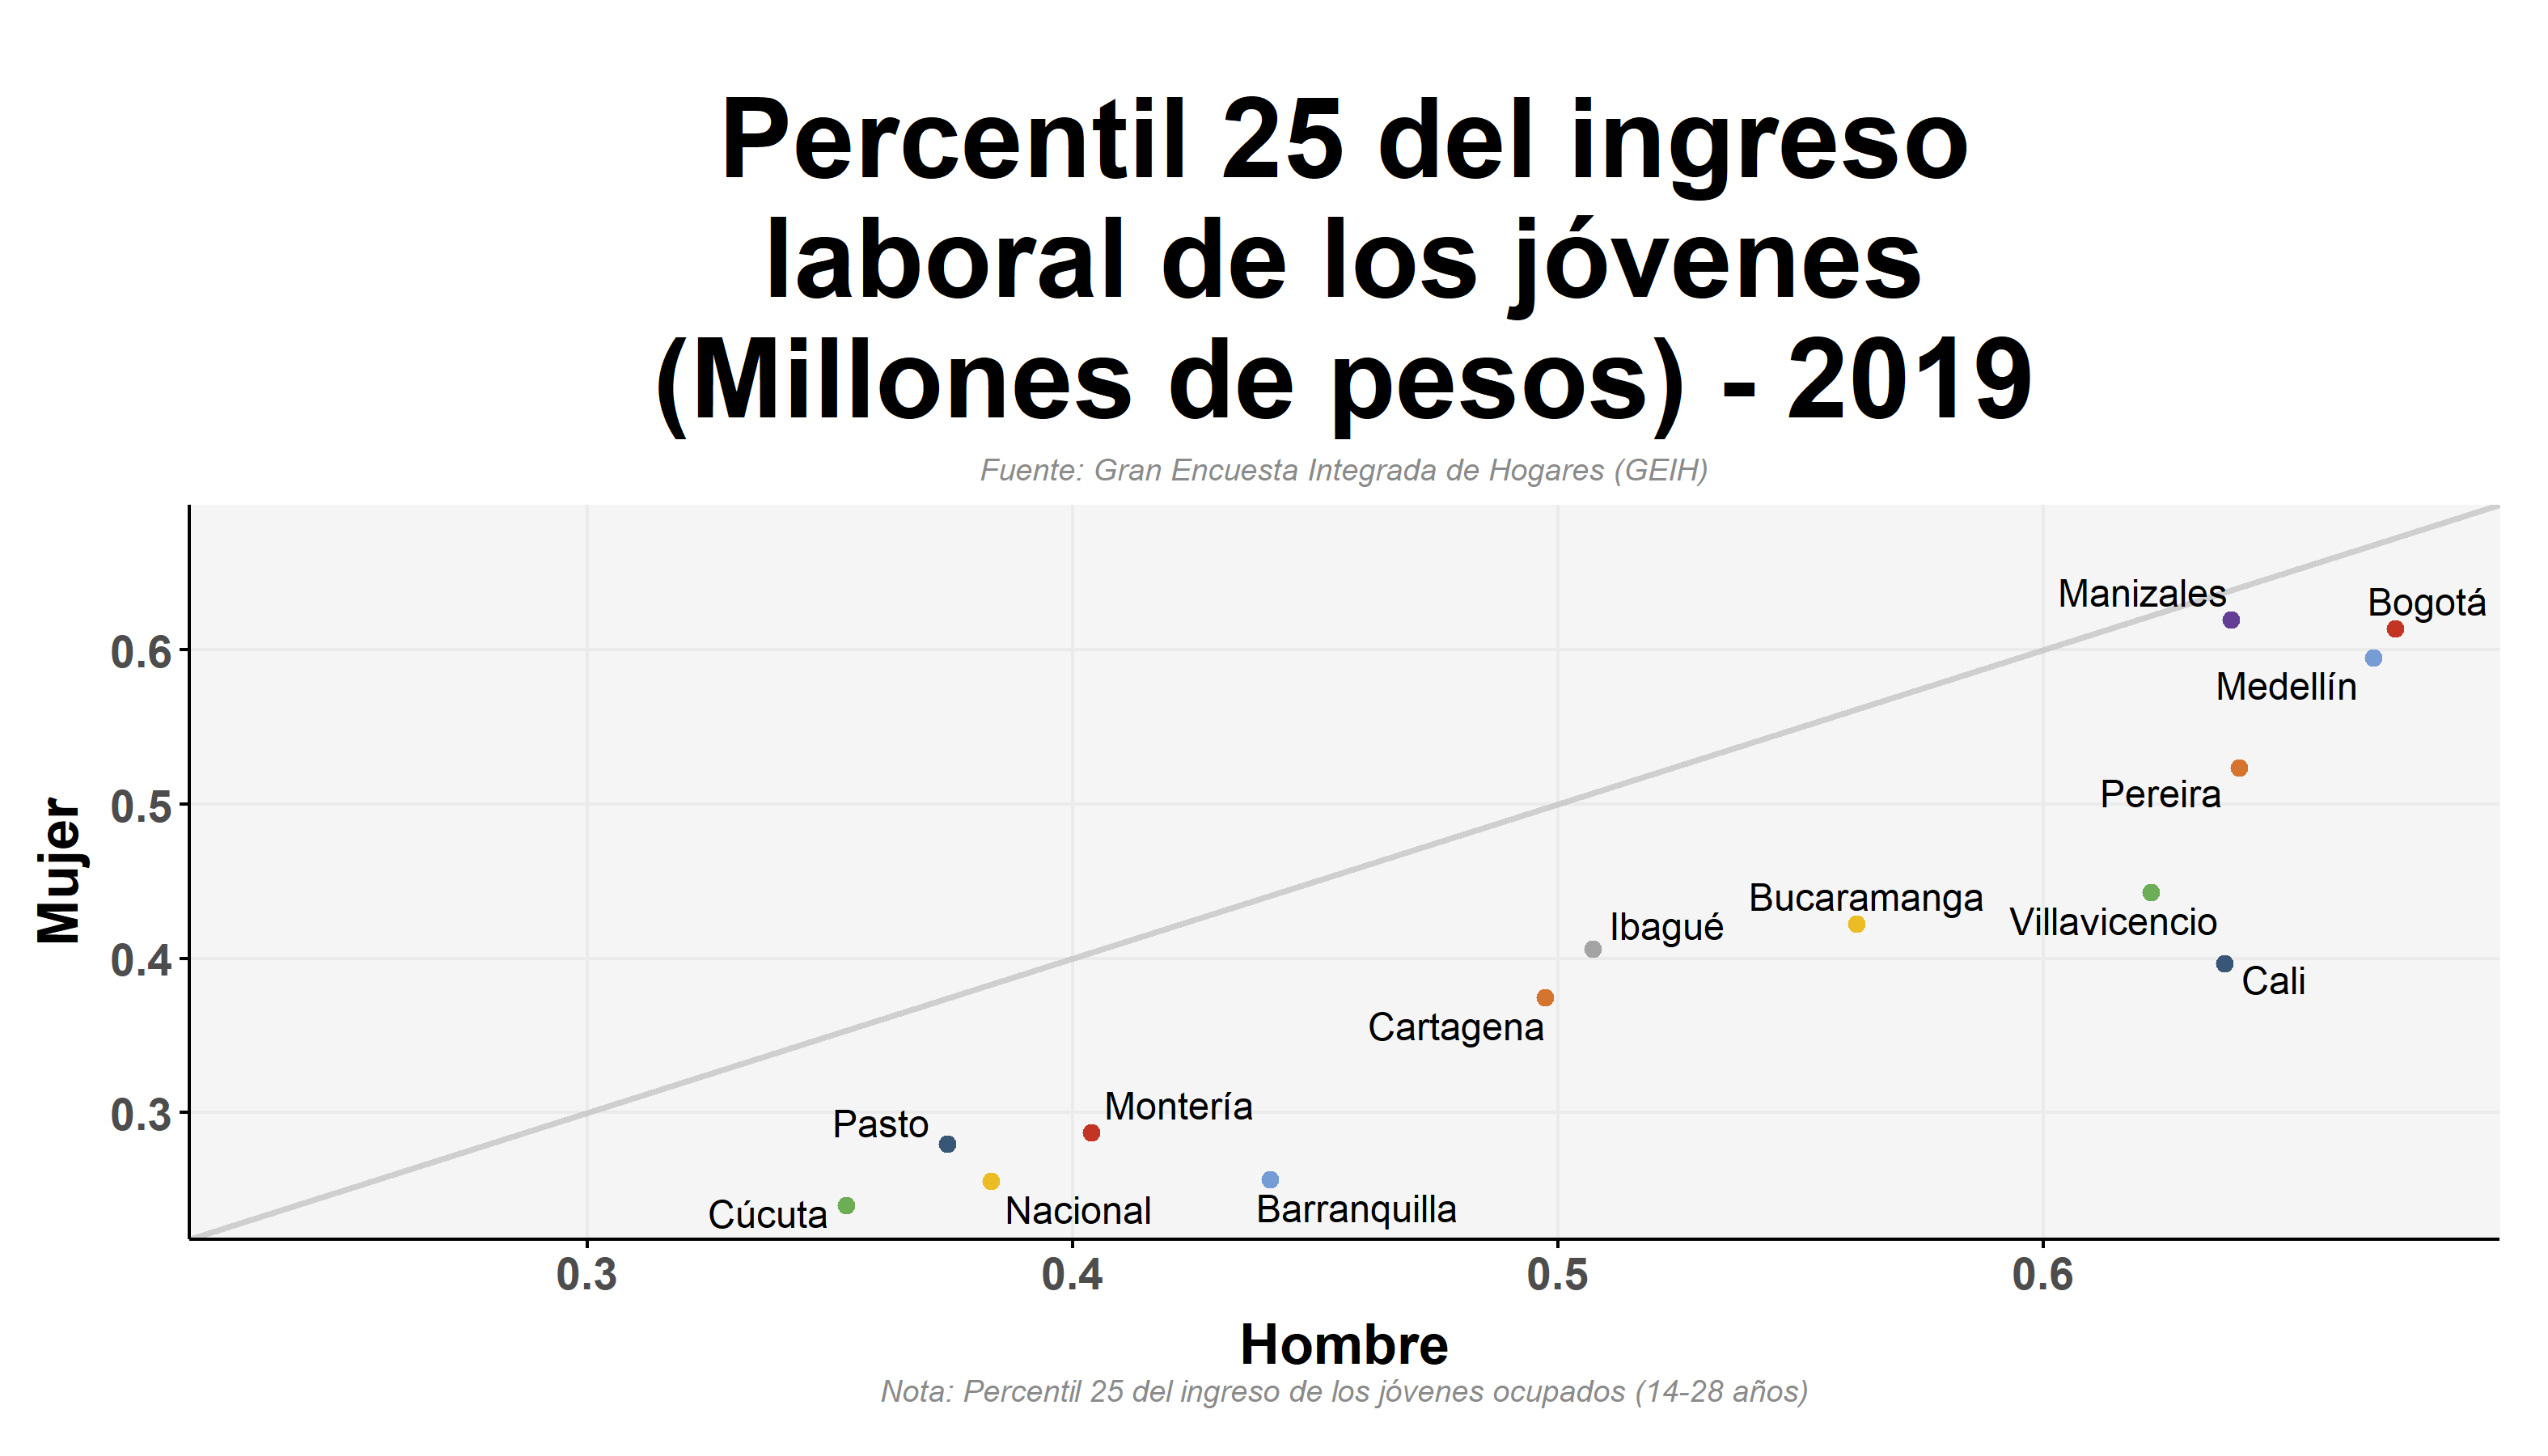
\includegraphics[width=\textwidth,keepaspectratio]{img/var_11_scatter.png}
        \end{center}
    \end{figure}
            \begin{itemize}
                \item Las minorías reciben mayor ingreso, aproximadamente 550 mil pesos, mientras que en las no minorías es de poco menos de 350 mil.
                \end{itemize}

%%%% Include figures
    \begin{figure}[H]
        \caption{Percentil 50 del ingreso laboral de los jóvenes a nivel nacional \label{map_result_2} }
        \begin{center}
        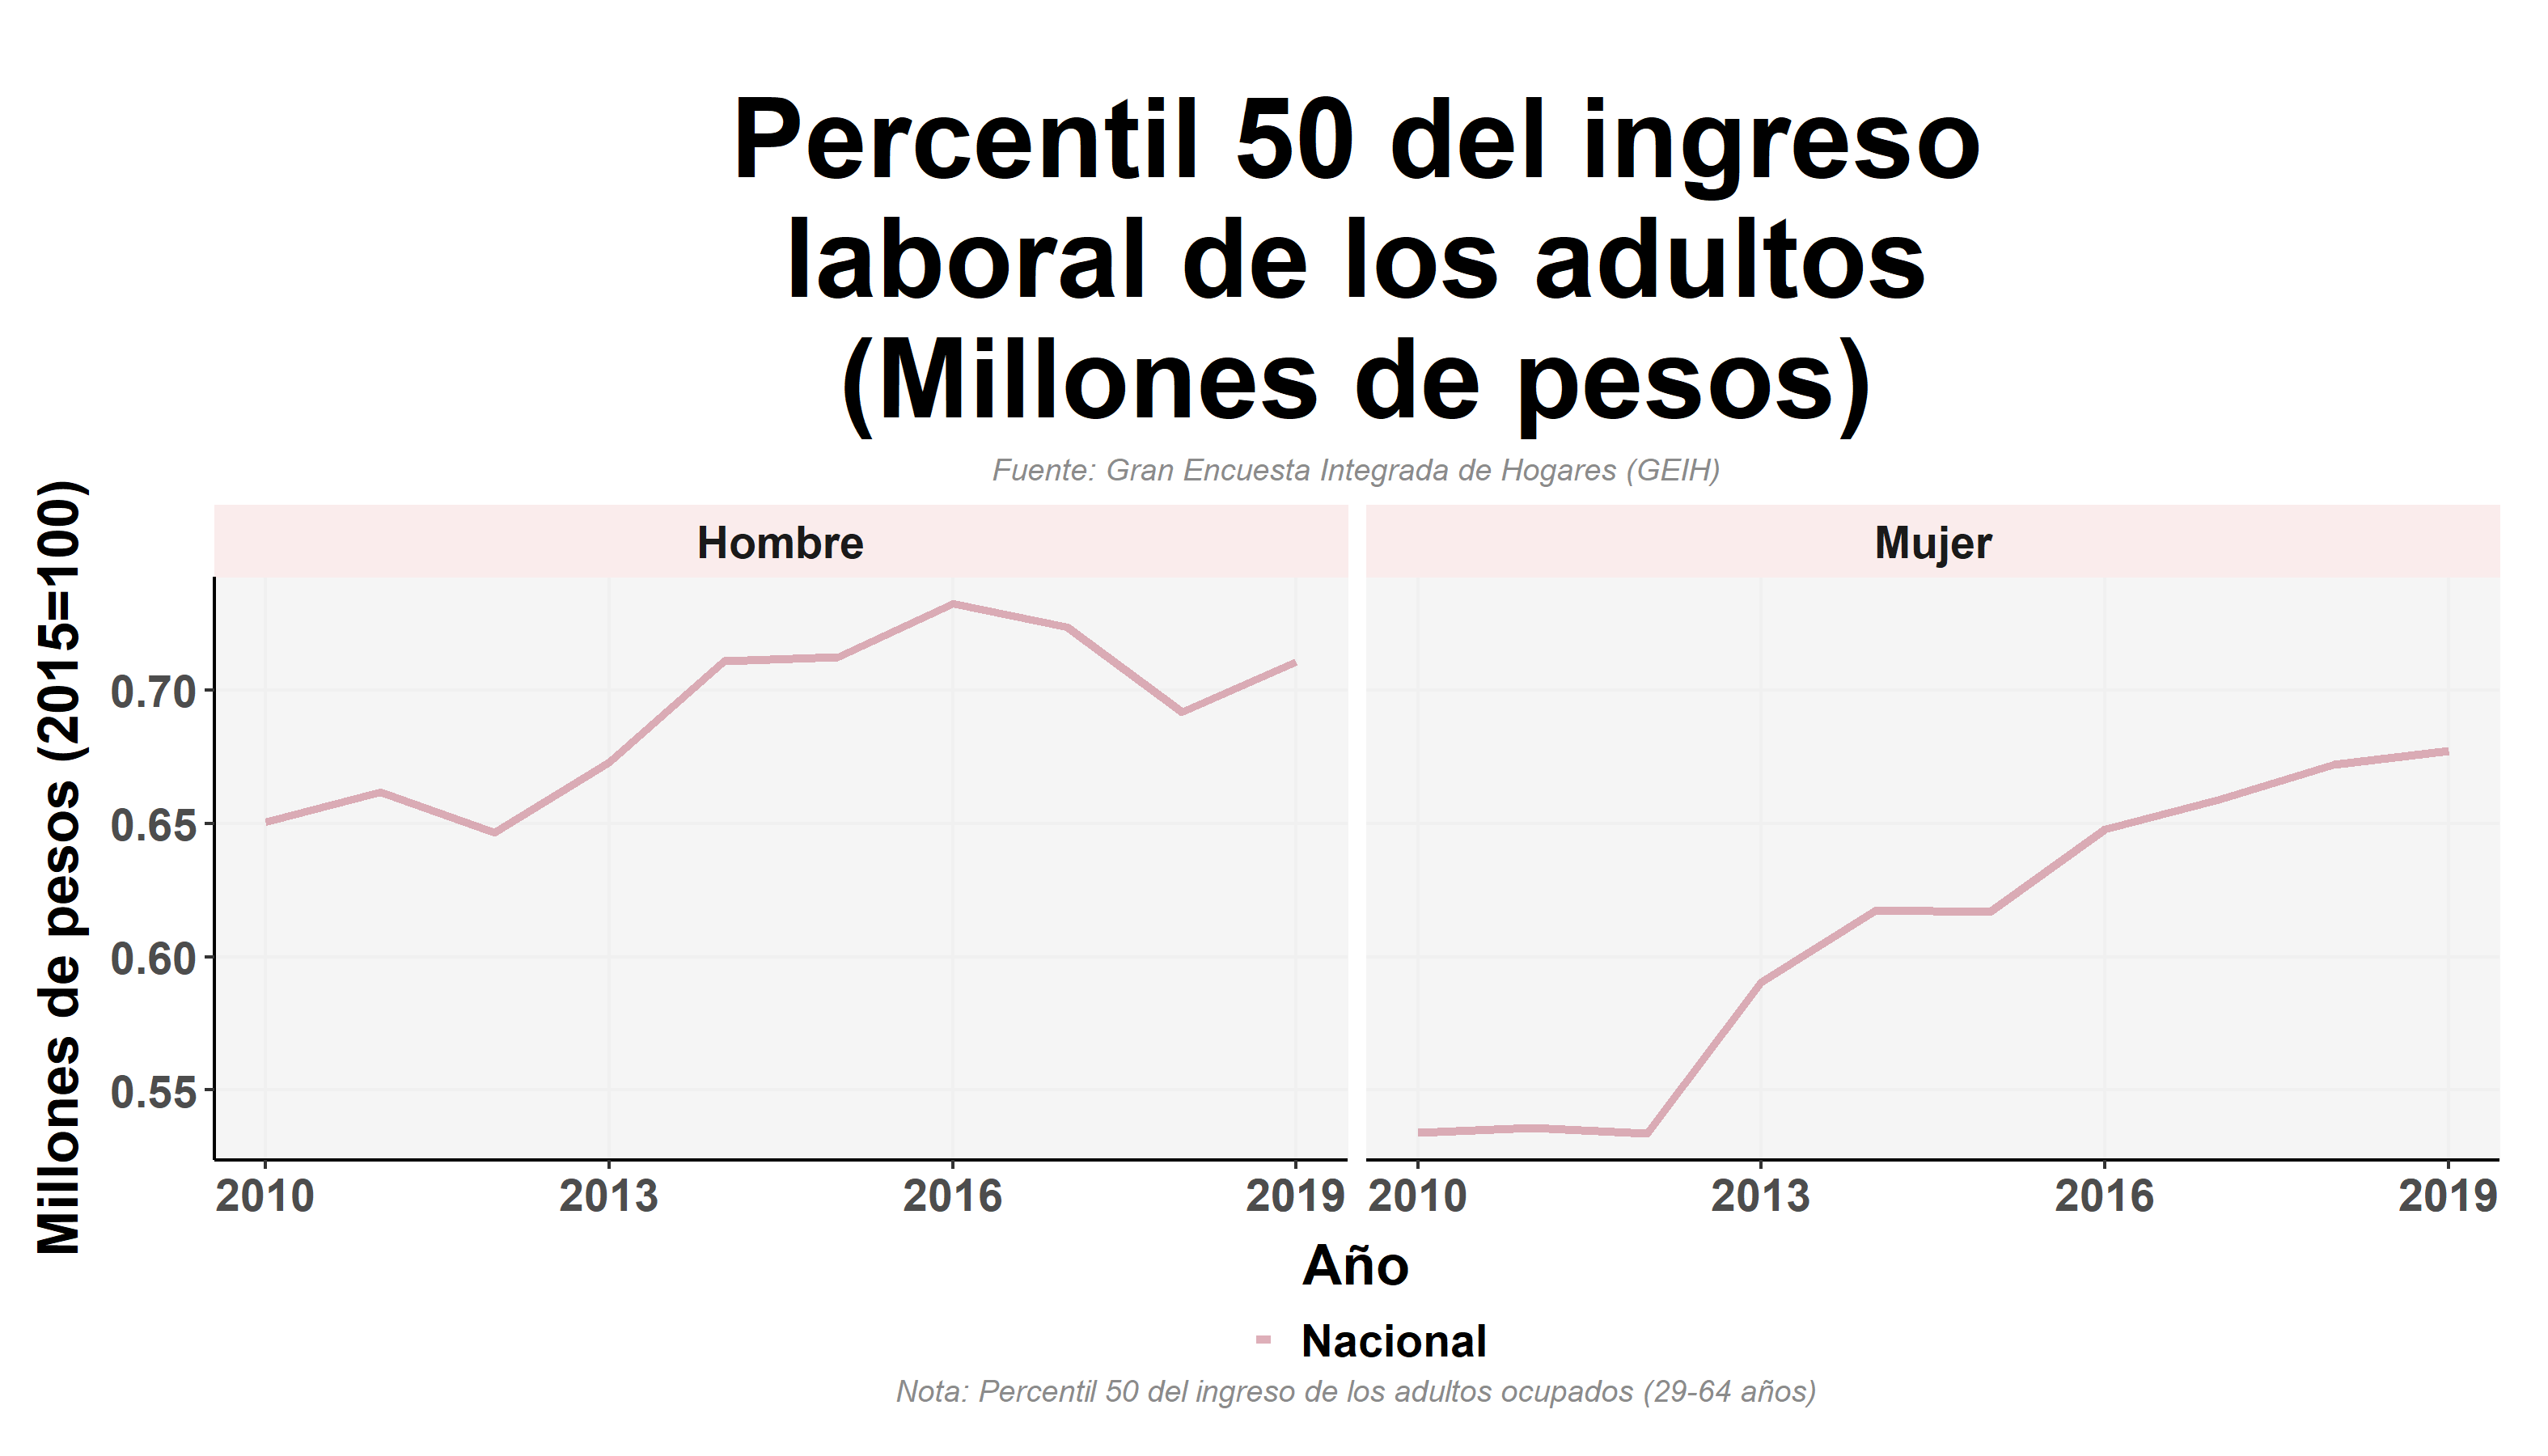
\includegraphics[width=\textwidth,keepaspectratio]{img/var_23_trend.png}
        \end{center}
    \end{figure}
            \begin{itemize}
                \item El ingreso en el percentil 50 de los jóvenes es aproximadamente el doble al ingreso en el percentil 25.
                \item Para el percentil 50 el ingreso ha venido aumentando constantemente desde el 2011.
                \end{itemize}

%%%% Include figures
    \begin{figure}[H]
        \caption{Percentil 50 del ingreso laboral de los jóvenes por género \label{map_result_2} }
        \begin{center}
        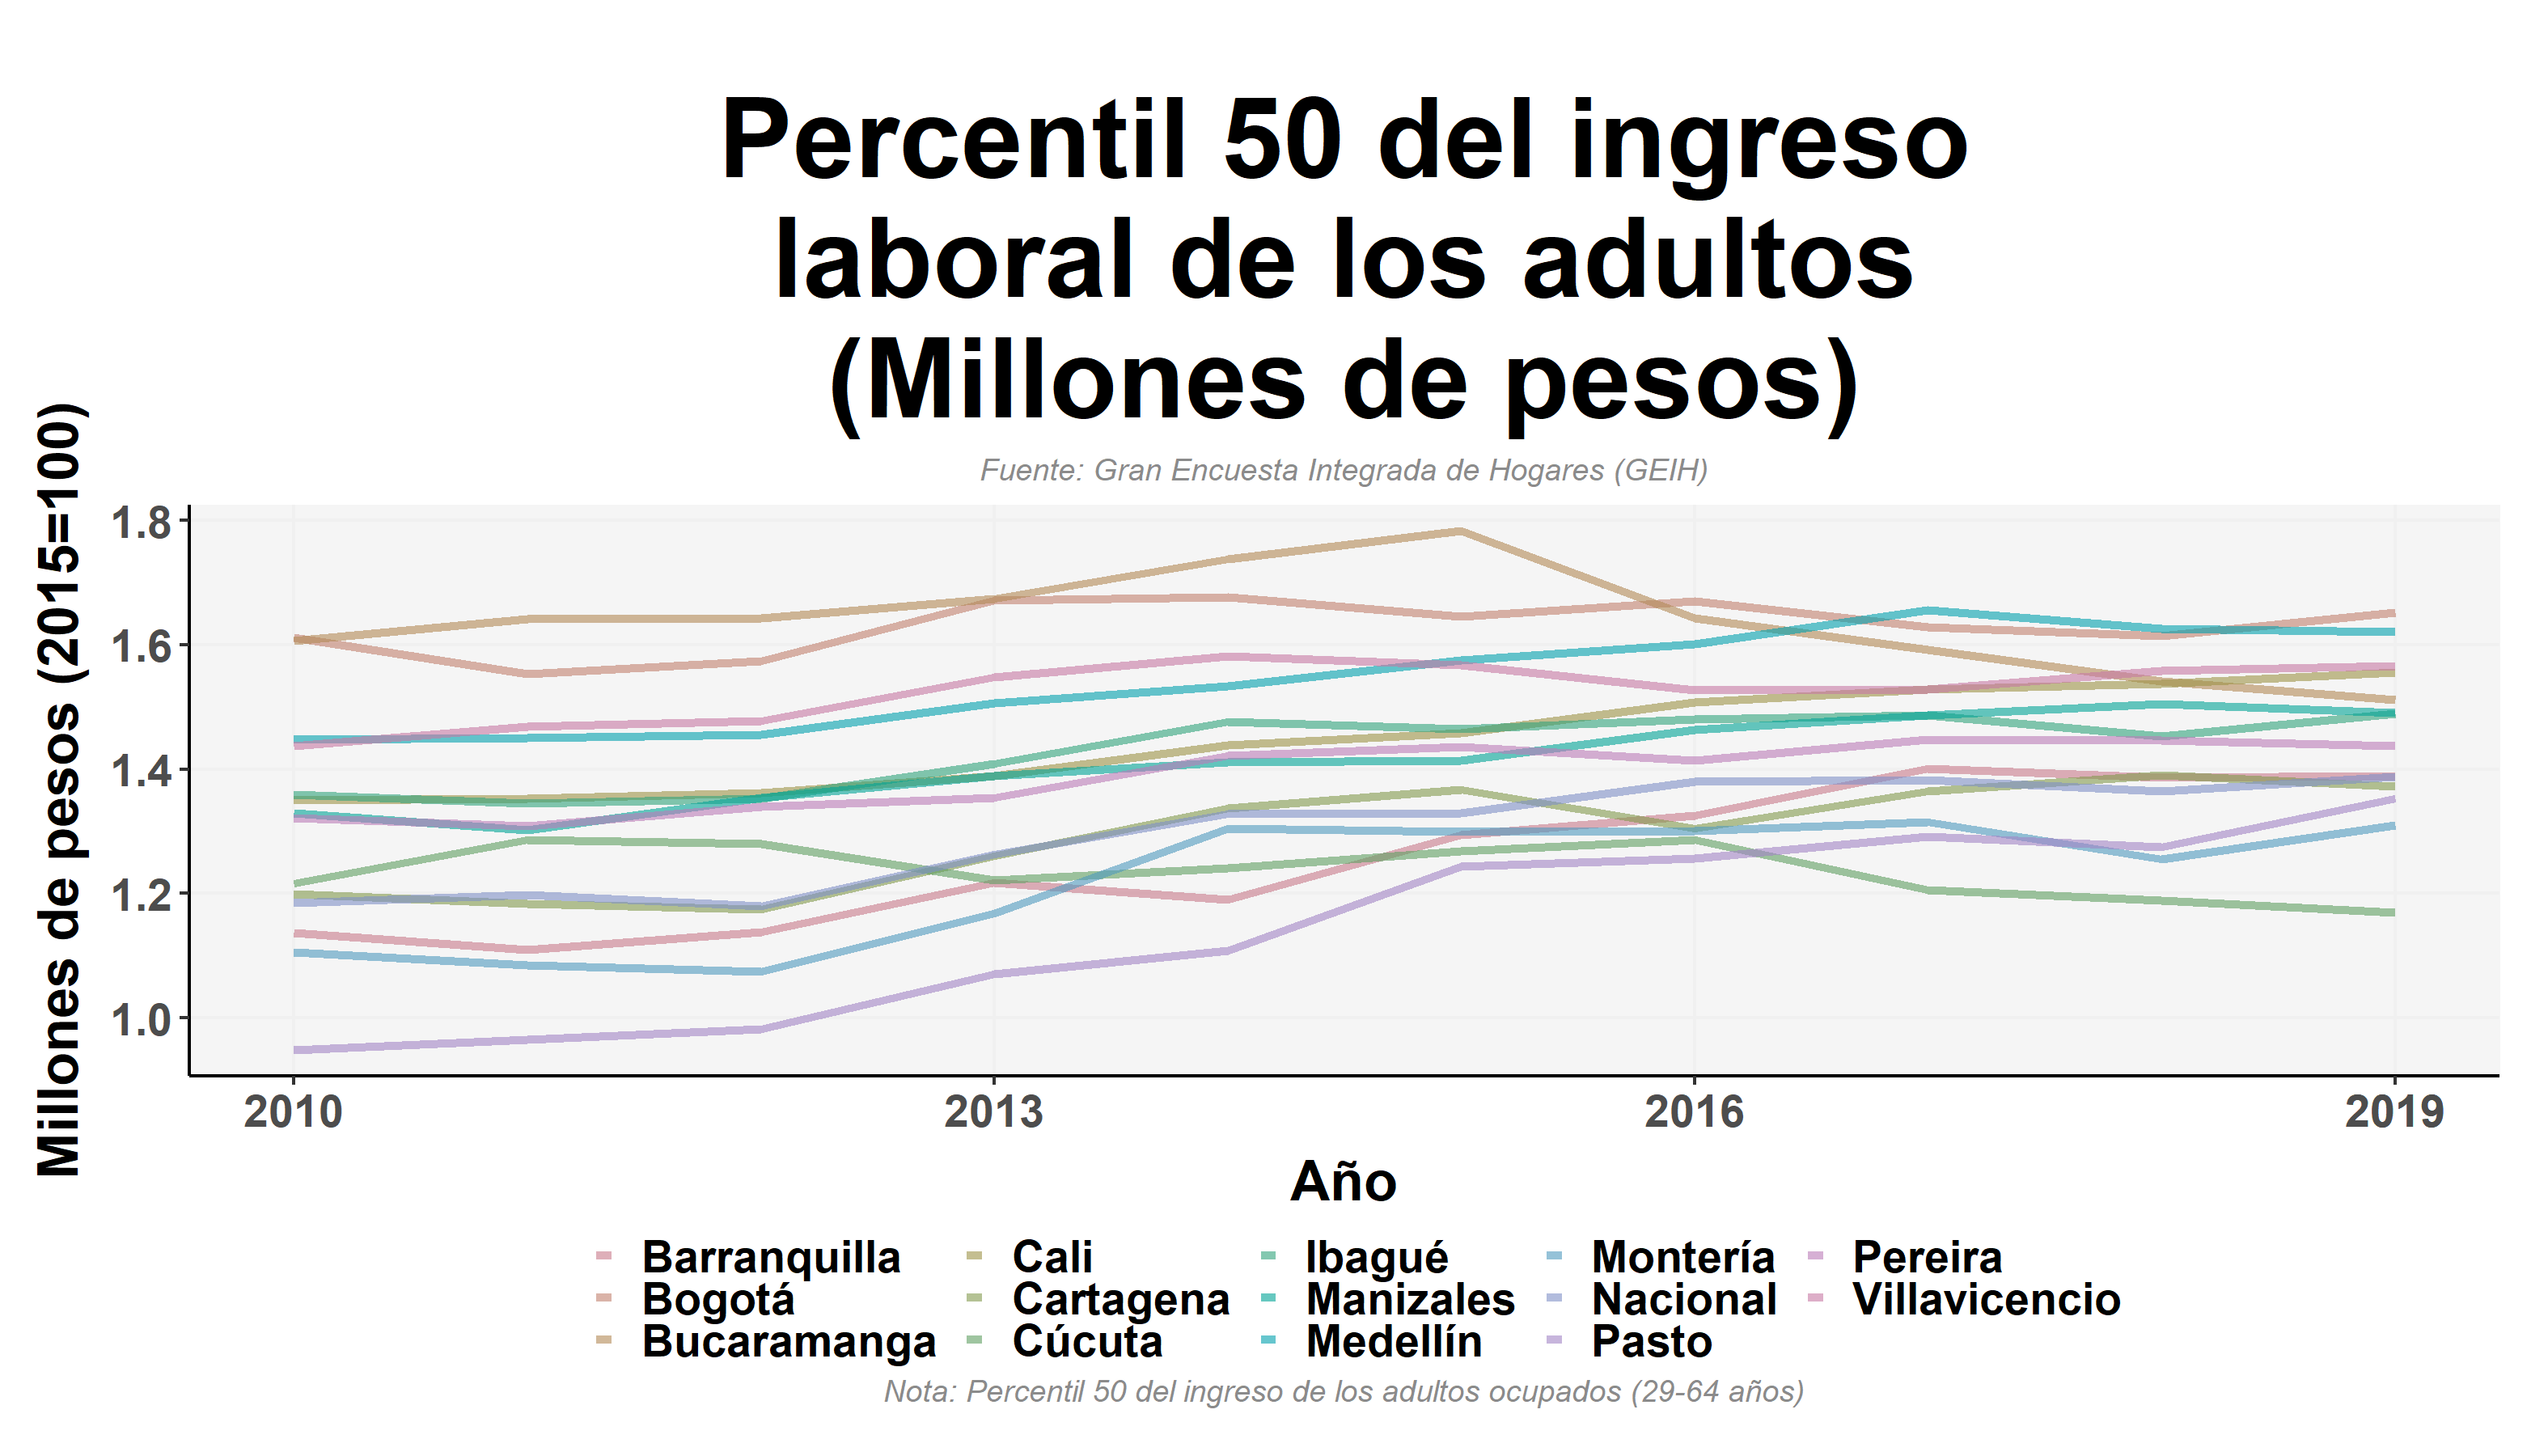
\includegraphics[width=\textwidth,keepaspectratio]{img/var_22_trend.png}
        \end{center}
    \end{figure}
            \begin{itemize}
                \item En el percentil 50 el ingreso de los jóvenes por género presenta niveles similares a partir del 2014 tanto para hombre como para mujer.
                \item Para ambos géneros se evidencia un aumento constante desde el 2011.
                \end{itemize}

%%%% Include figures
    \begin{figure}[H]
        \caption{Percentil 50 del ingreso laboral de los jóvenes por minorías y no minorías para 2020 \label{map_result_2} }
        \begin{center}
        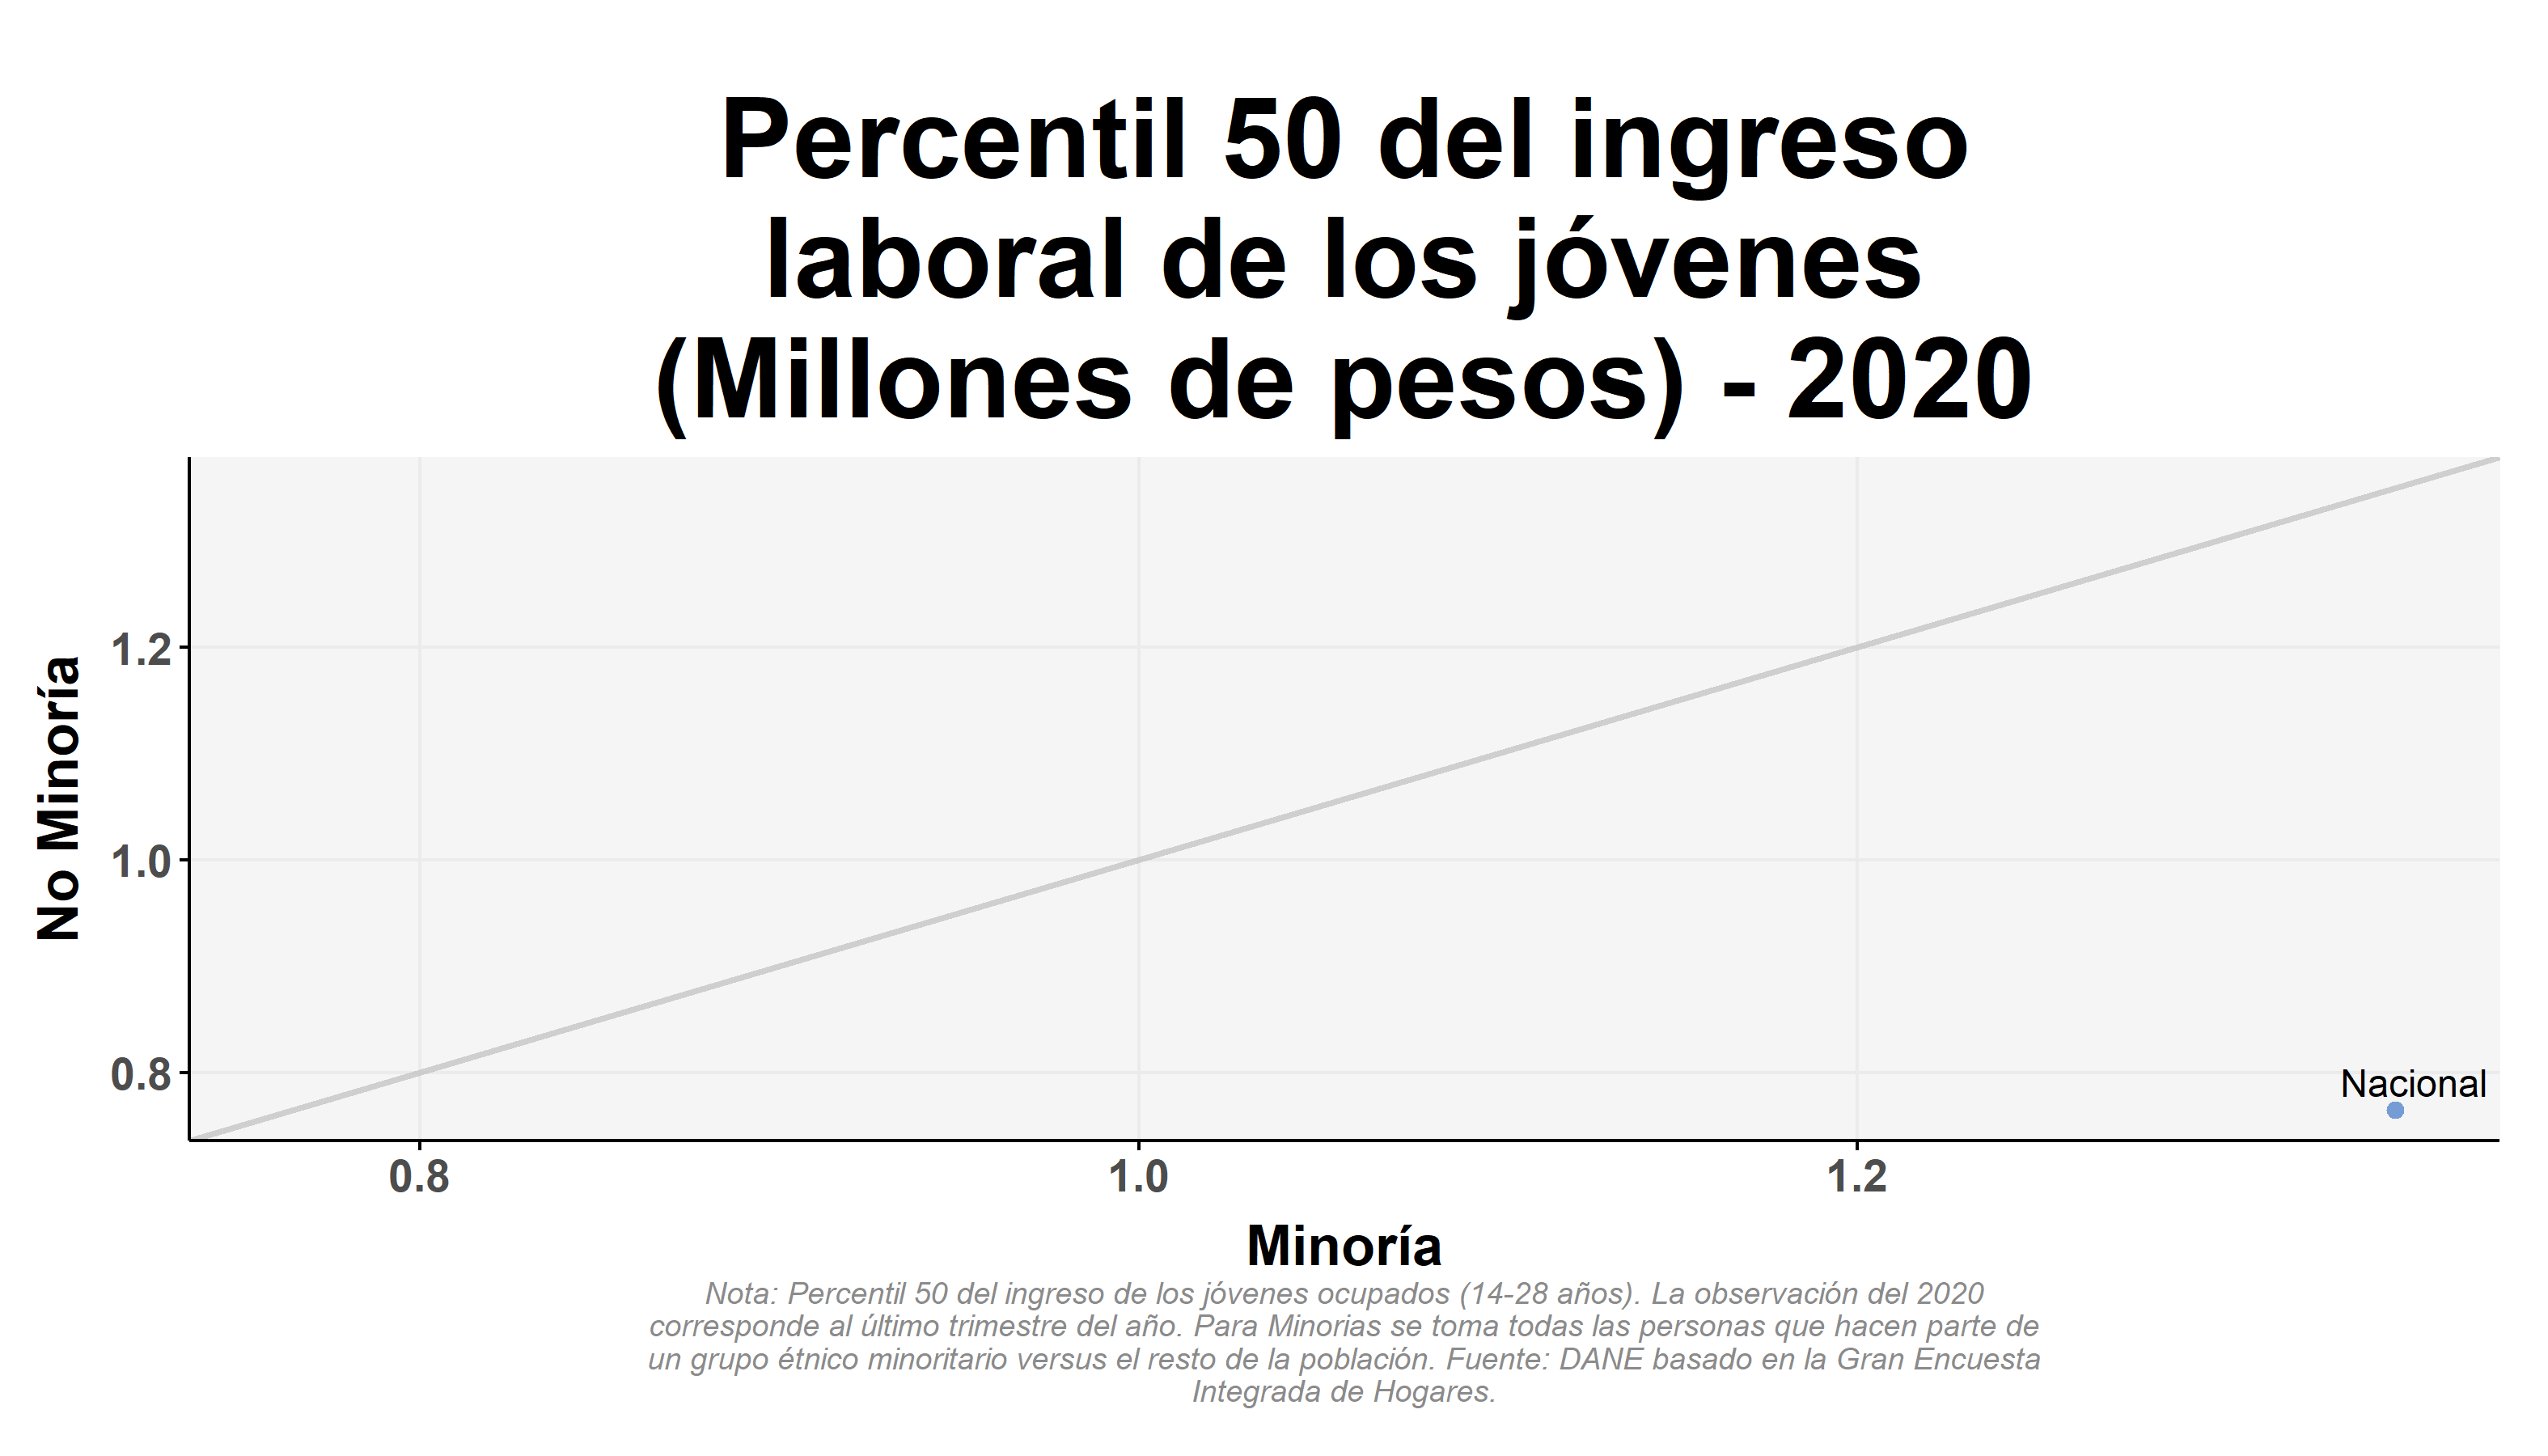
\includegraphics[width=\textwidth,keepaspectratio]{img/var_21_scatter.png}
        \end{center}
    \end{figure}
            \begin{itemize}
                \item El ingreso laboral en el percentil 50 es mayor para las minorías que las no minorías, siendo una diferencia de alrededor de 500 mil pesos.
                \end{itemize}

%%%% Include figures
    \begin{figure}[H]
        \caption{Percentil 75 del ingreso laboral de los jóvenes a nivel nacional \label{map_result_2} }
        \begin{center}
        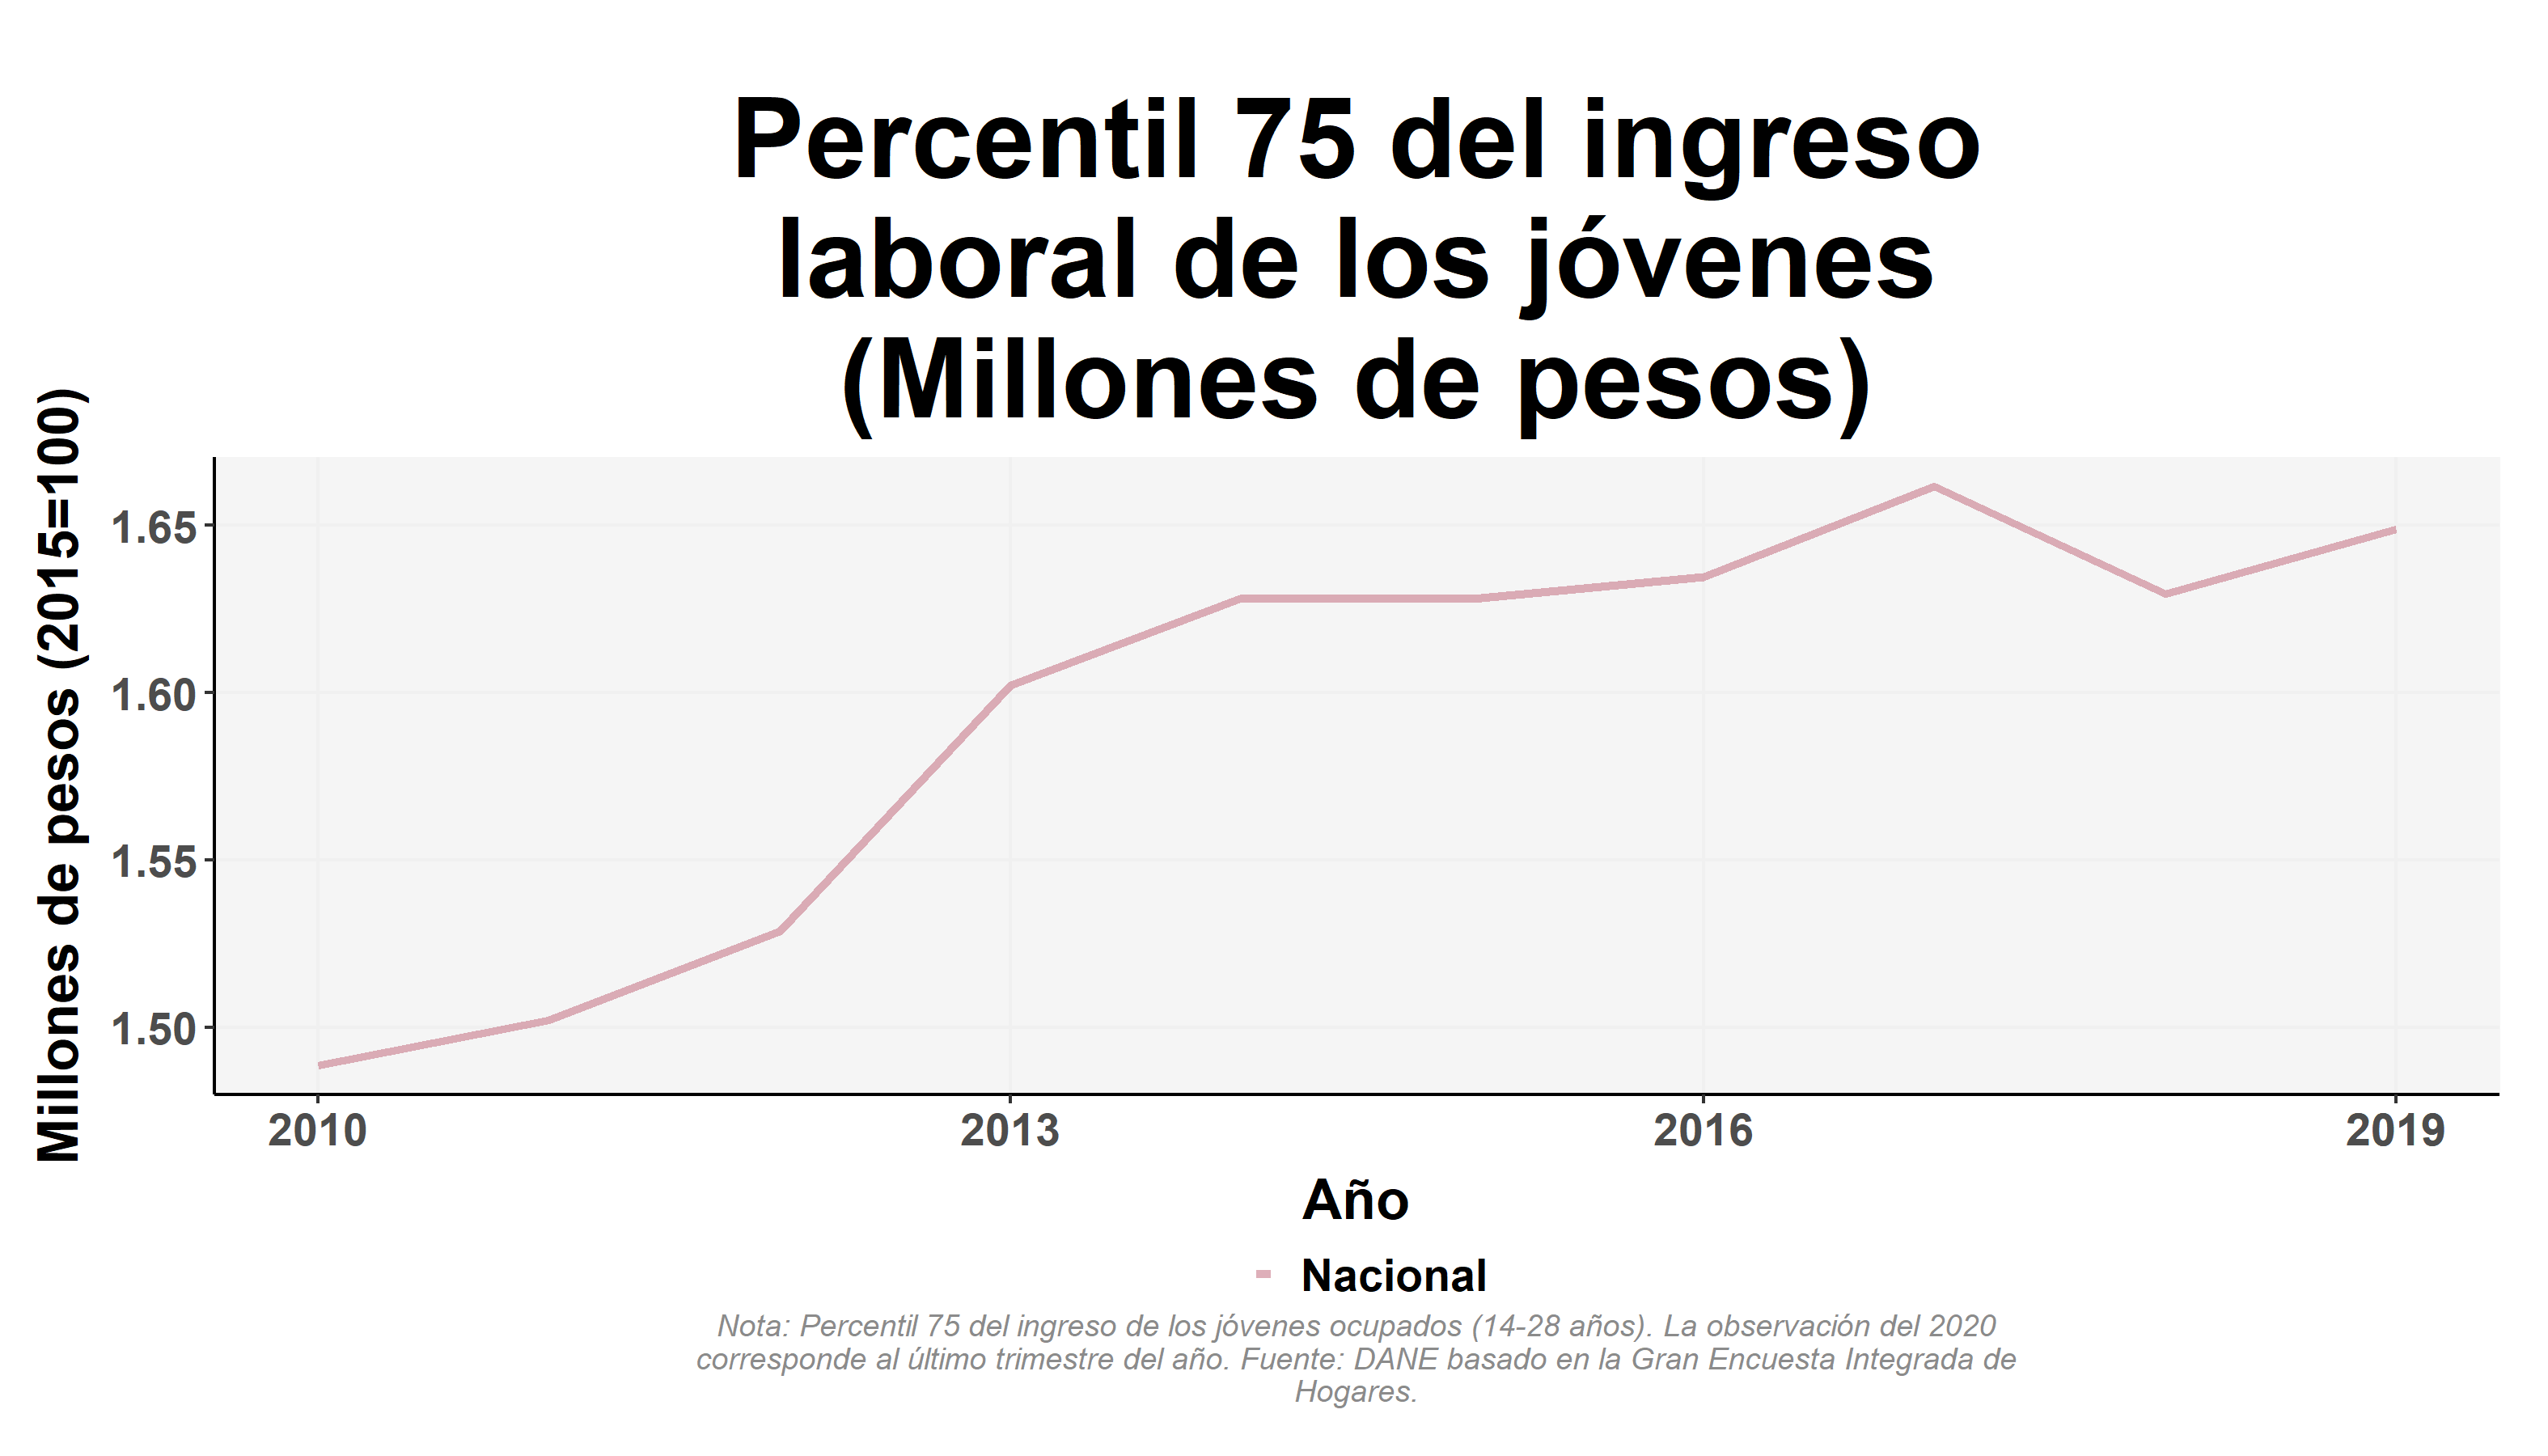
\includegraphics[width=\textwidth,keepaspectratio]{img/var_33_trend.png}
        \end{center}
    \end{figure}
            \begin{itemize}
                \item El ingreso de los jóvenes en el percentil 75 estuvo en aumento desde el 2010 hasta el 2017, para 2019 tiene un retroceso a los valores del 2016.
                \item Para 2019 aumentó el ingreso pero aún no se recuperó los niveles de 2017.
                \end{itemize}

%%%% Include figures
    \begin{figure}[H]
        \caption{Percentil 75 del ingreso laboral de los jóvenes por género \label{map_result_2} }
        \begin{center}
        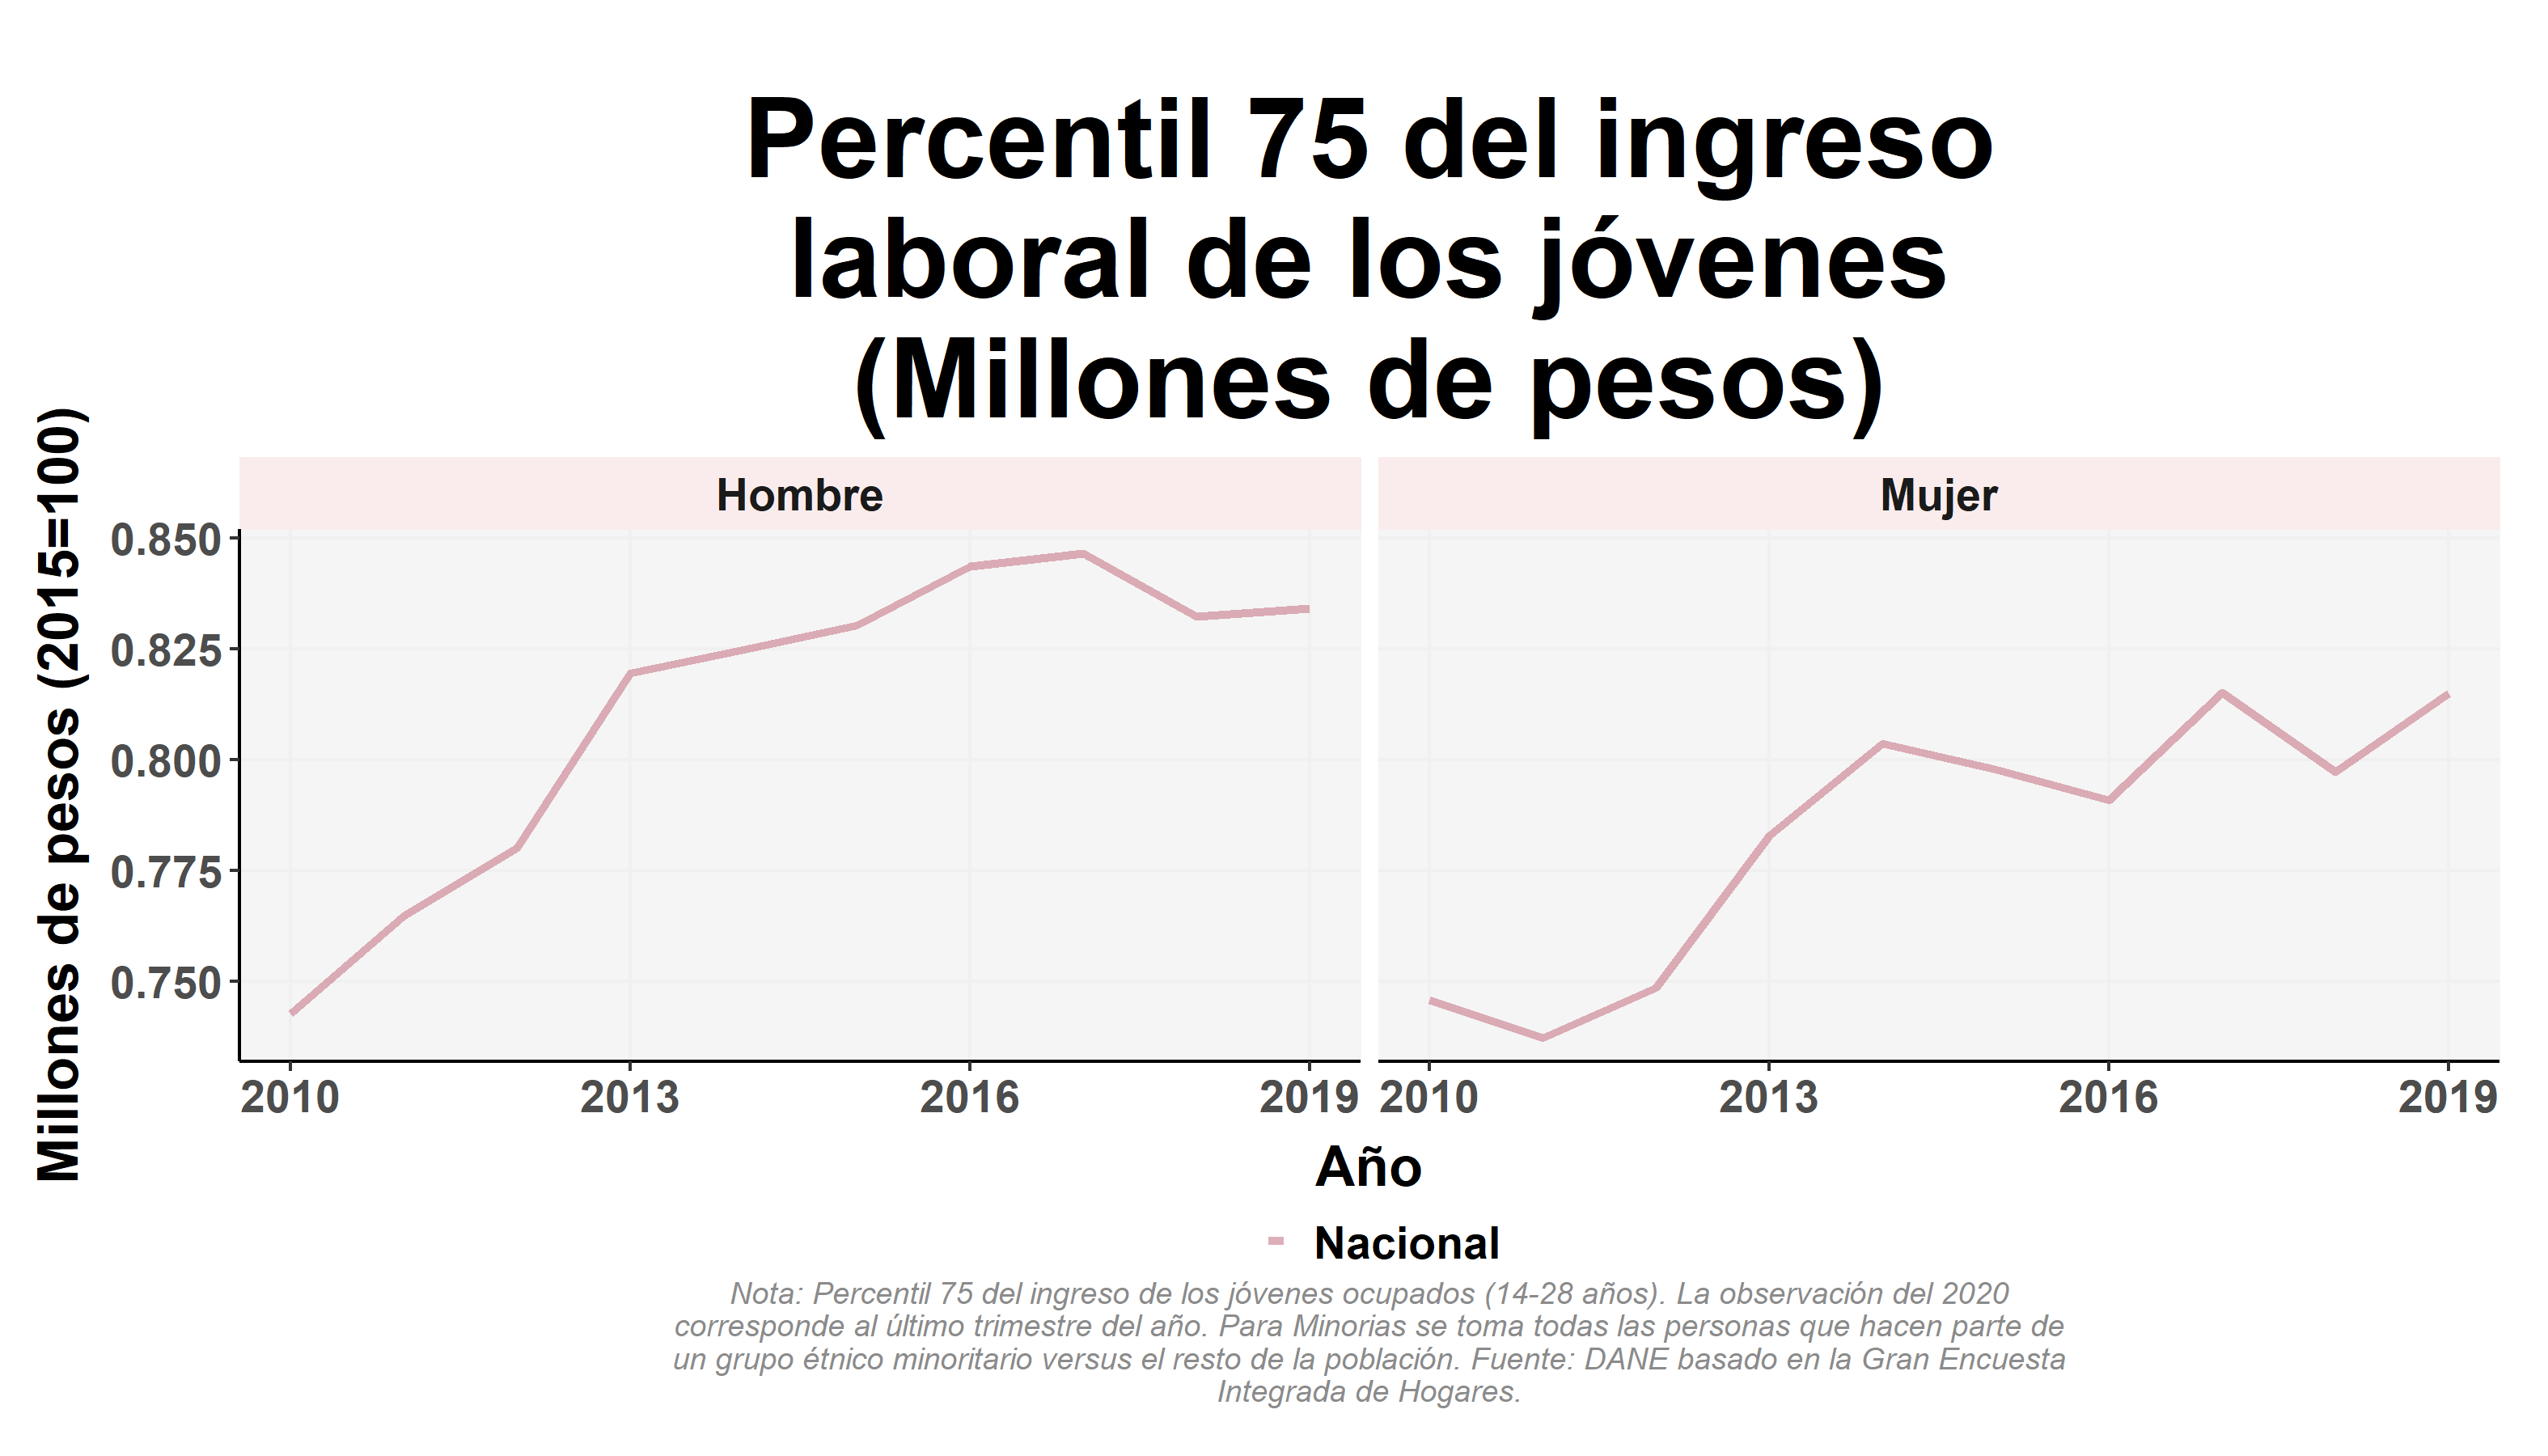
\includegraphics[width=\textwidth,keepaspectratio]{img/var_32_trend.png}
        \end{center}
    \end{figure}
            \begin{itemize}
                \item La brecha de ingreso por género en el percentil 75 es mayor a la del 50, pero menor a la del 25.
                \item El ingreso ha aumentado de manera constante para el hombre hasta 2017, en el caso de la mujer aumentó hasta 2014 y a partir de ahí inició a fluctuar aún más.
                \end{itemize}

%%%% Include figures
    \begin{figure}[H]
        \caption{Percentil 75 del ingreso laboral de los jóvenes por minorías y no minorías para 2020 \label{map_result_2} }
        \begin{center}
        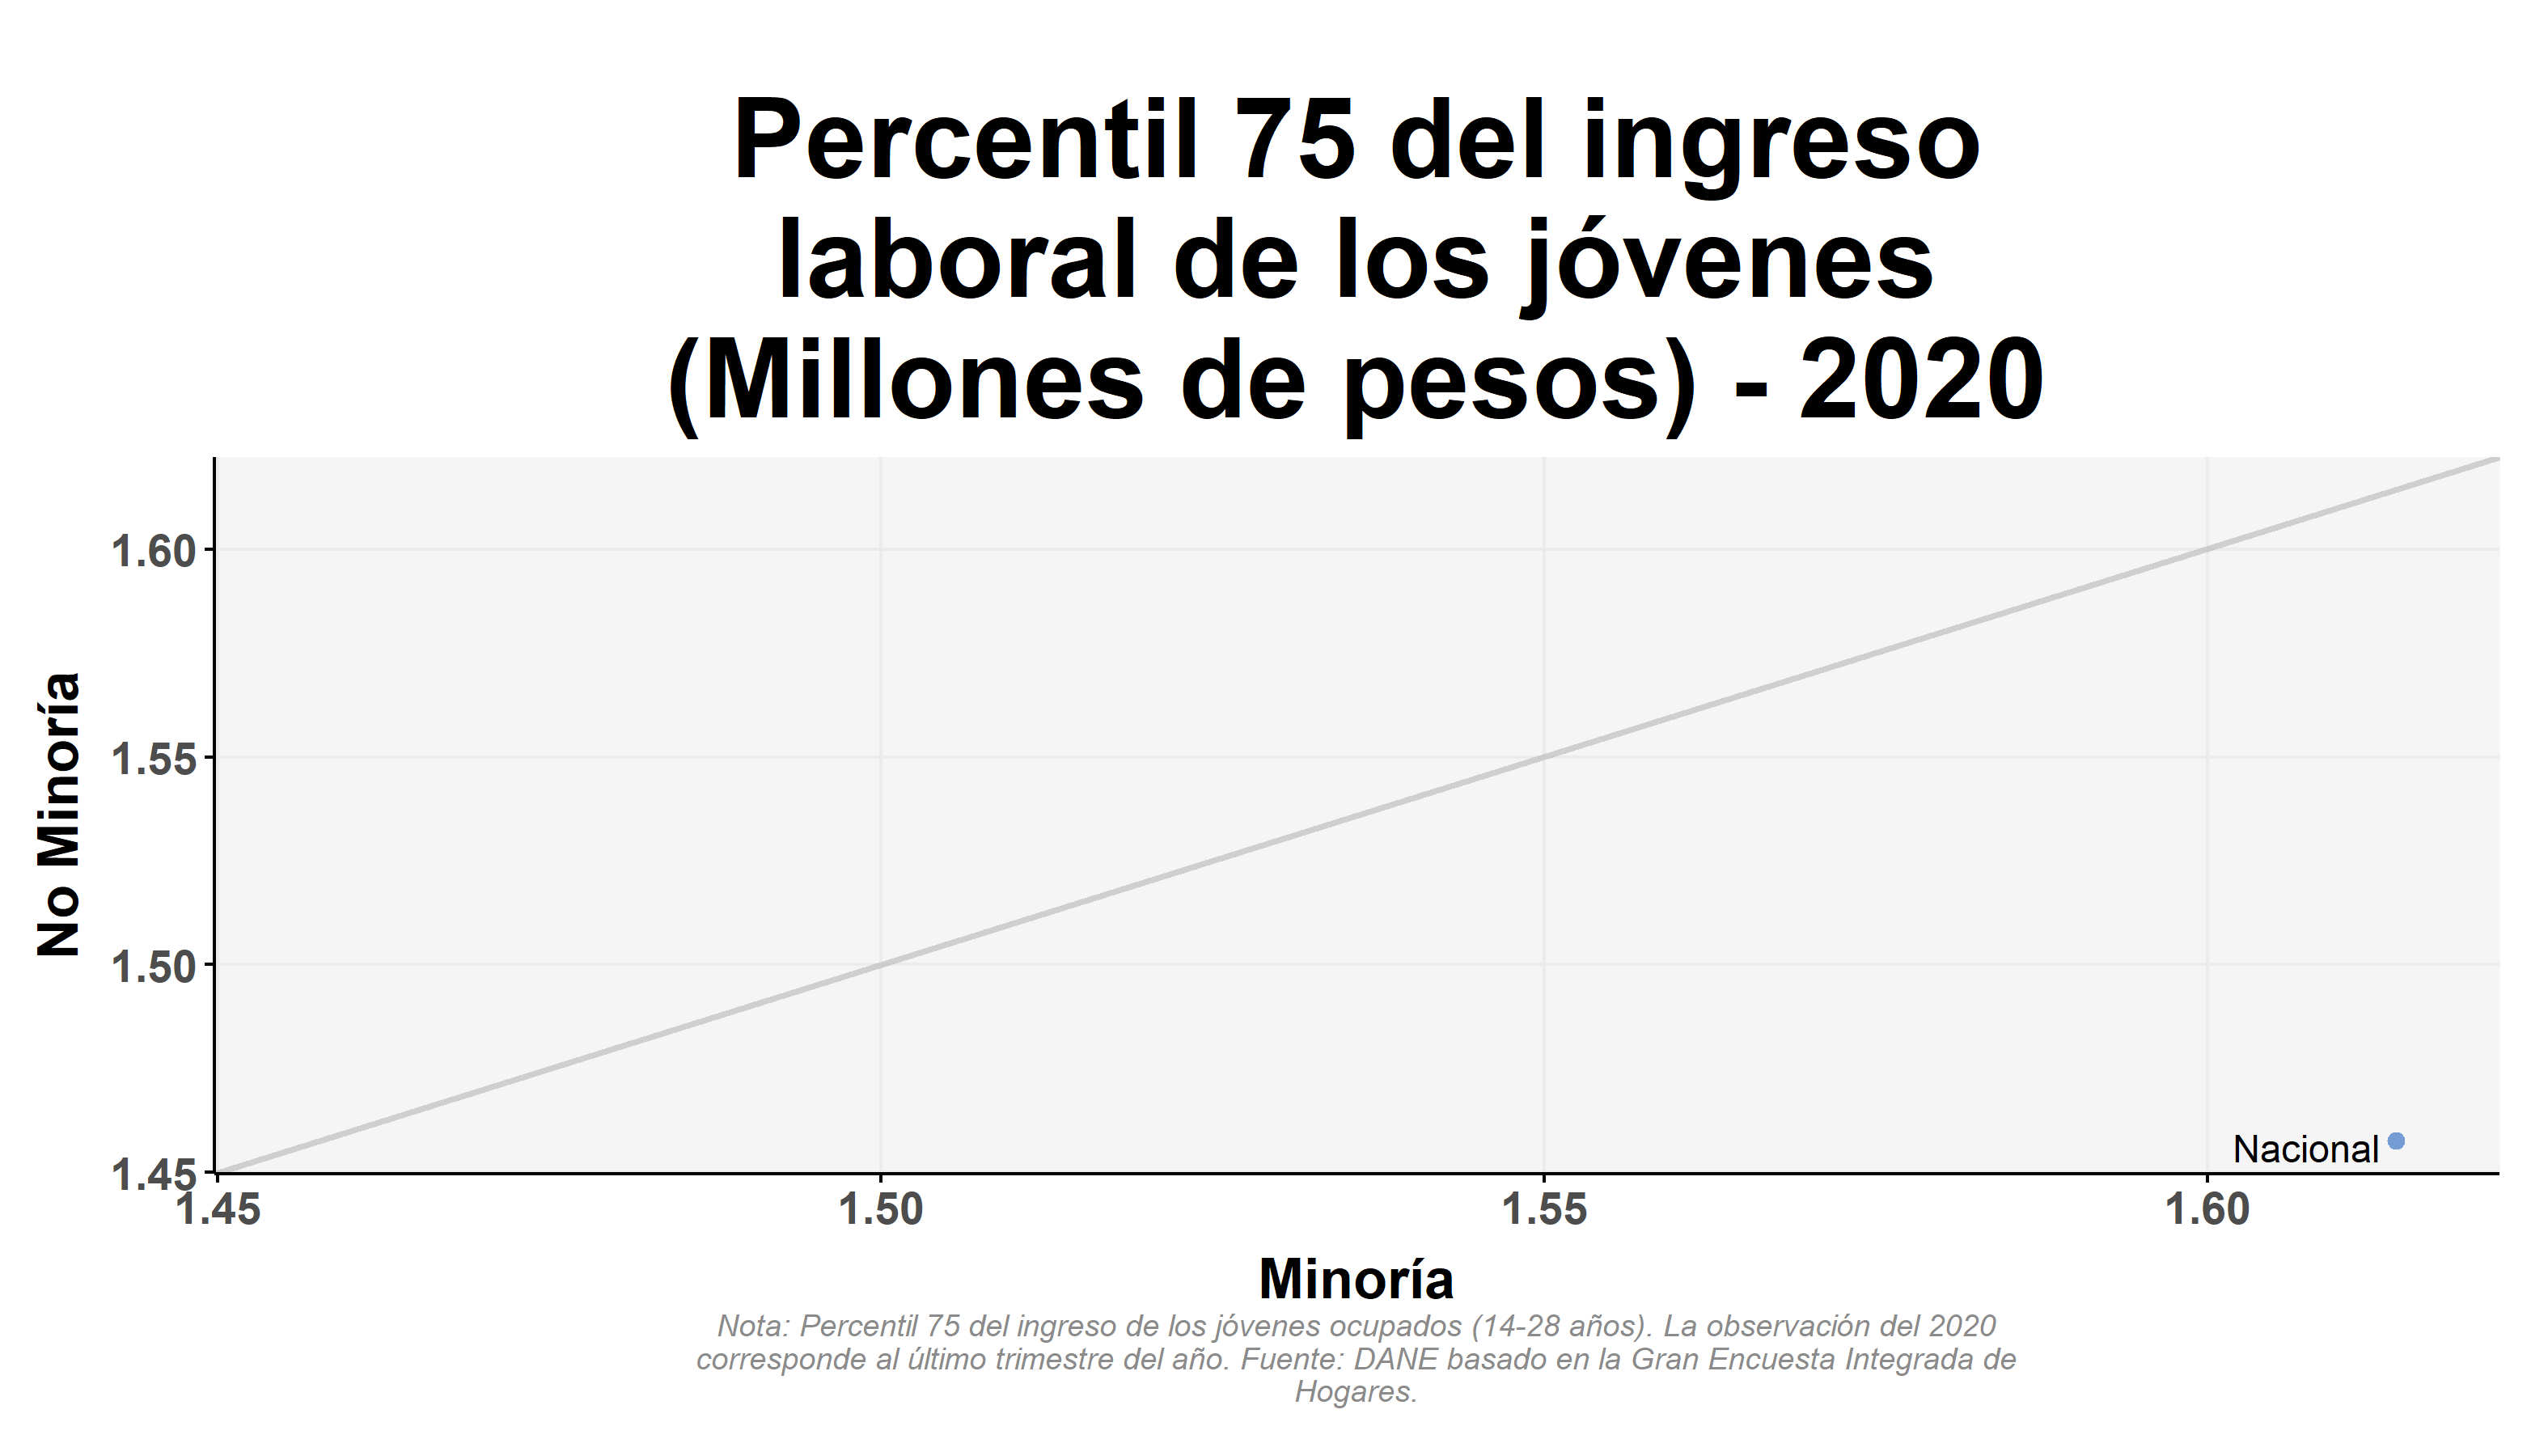
\includegraphics[width=\textwidth,keepaspectratio]{img/var_31_scatter.png}
        \end{center}
    \end{figure}
            \begin{itemize}
                \item El ingreso en el percentil 75 es mayor para las minorías que para las no minorías, con una diferencia aproximadamente de 100 mil pesos.
                \end{itemize}

\section{Adultez}
    \subsection{Desempleo}
        \subsubsection{Personas que no estudian ni trabajan}

%%%% Include figures
    \begin{figure}[H]
        \caption{Personas que no estudian ni trabajan a nivel nacional \label{map_result_2} }
        \begin{center}
        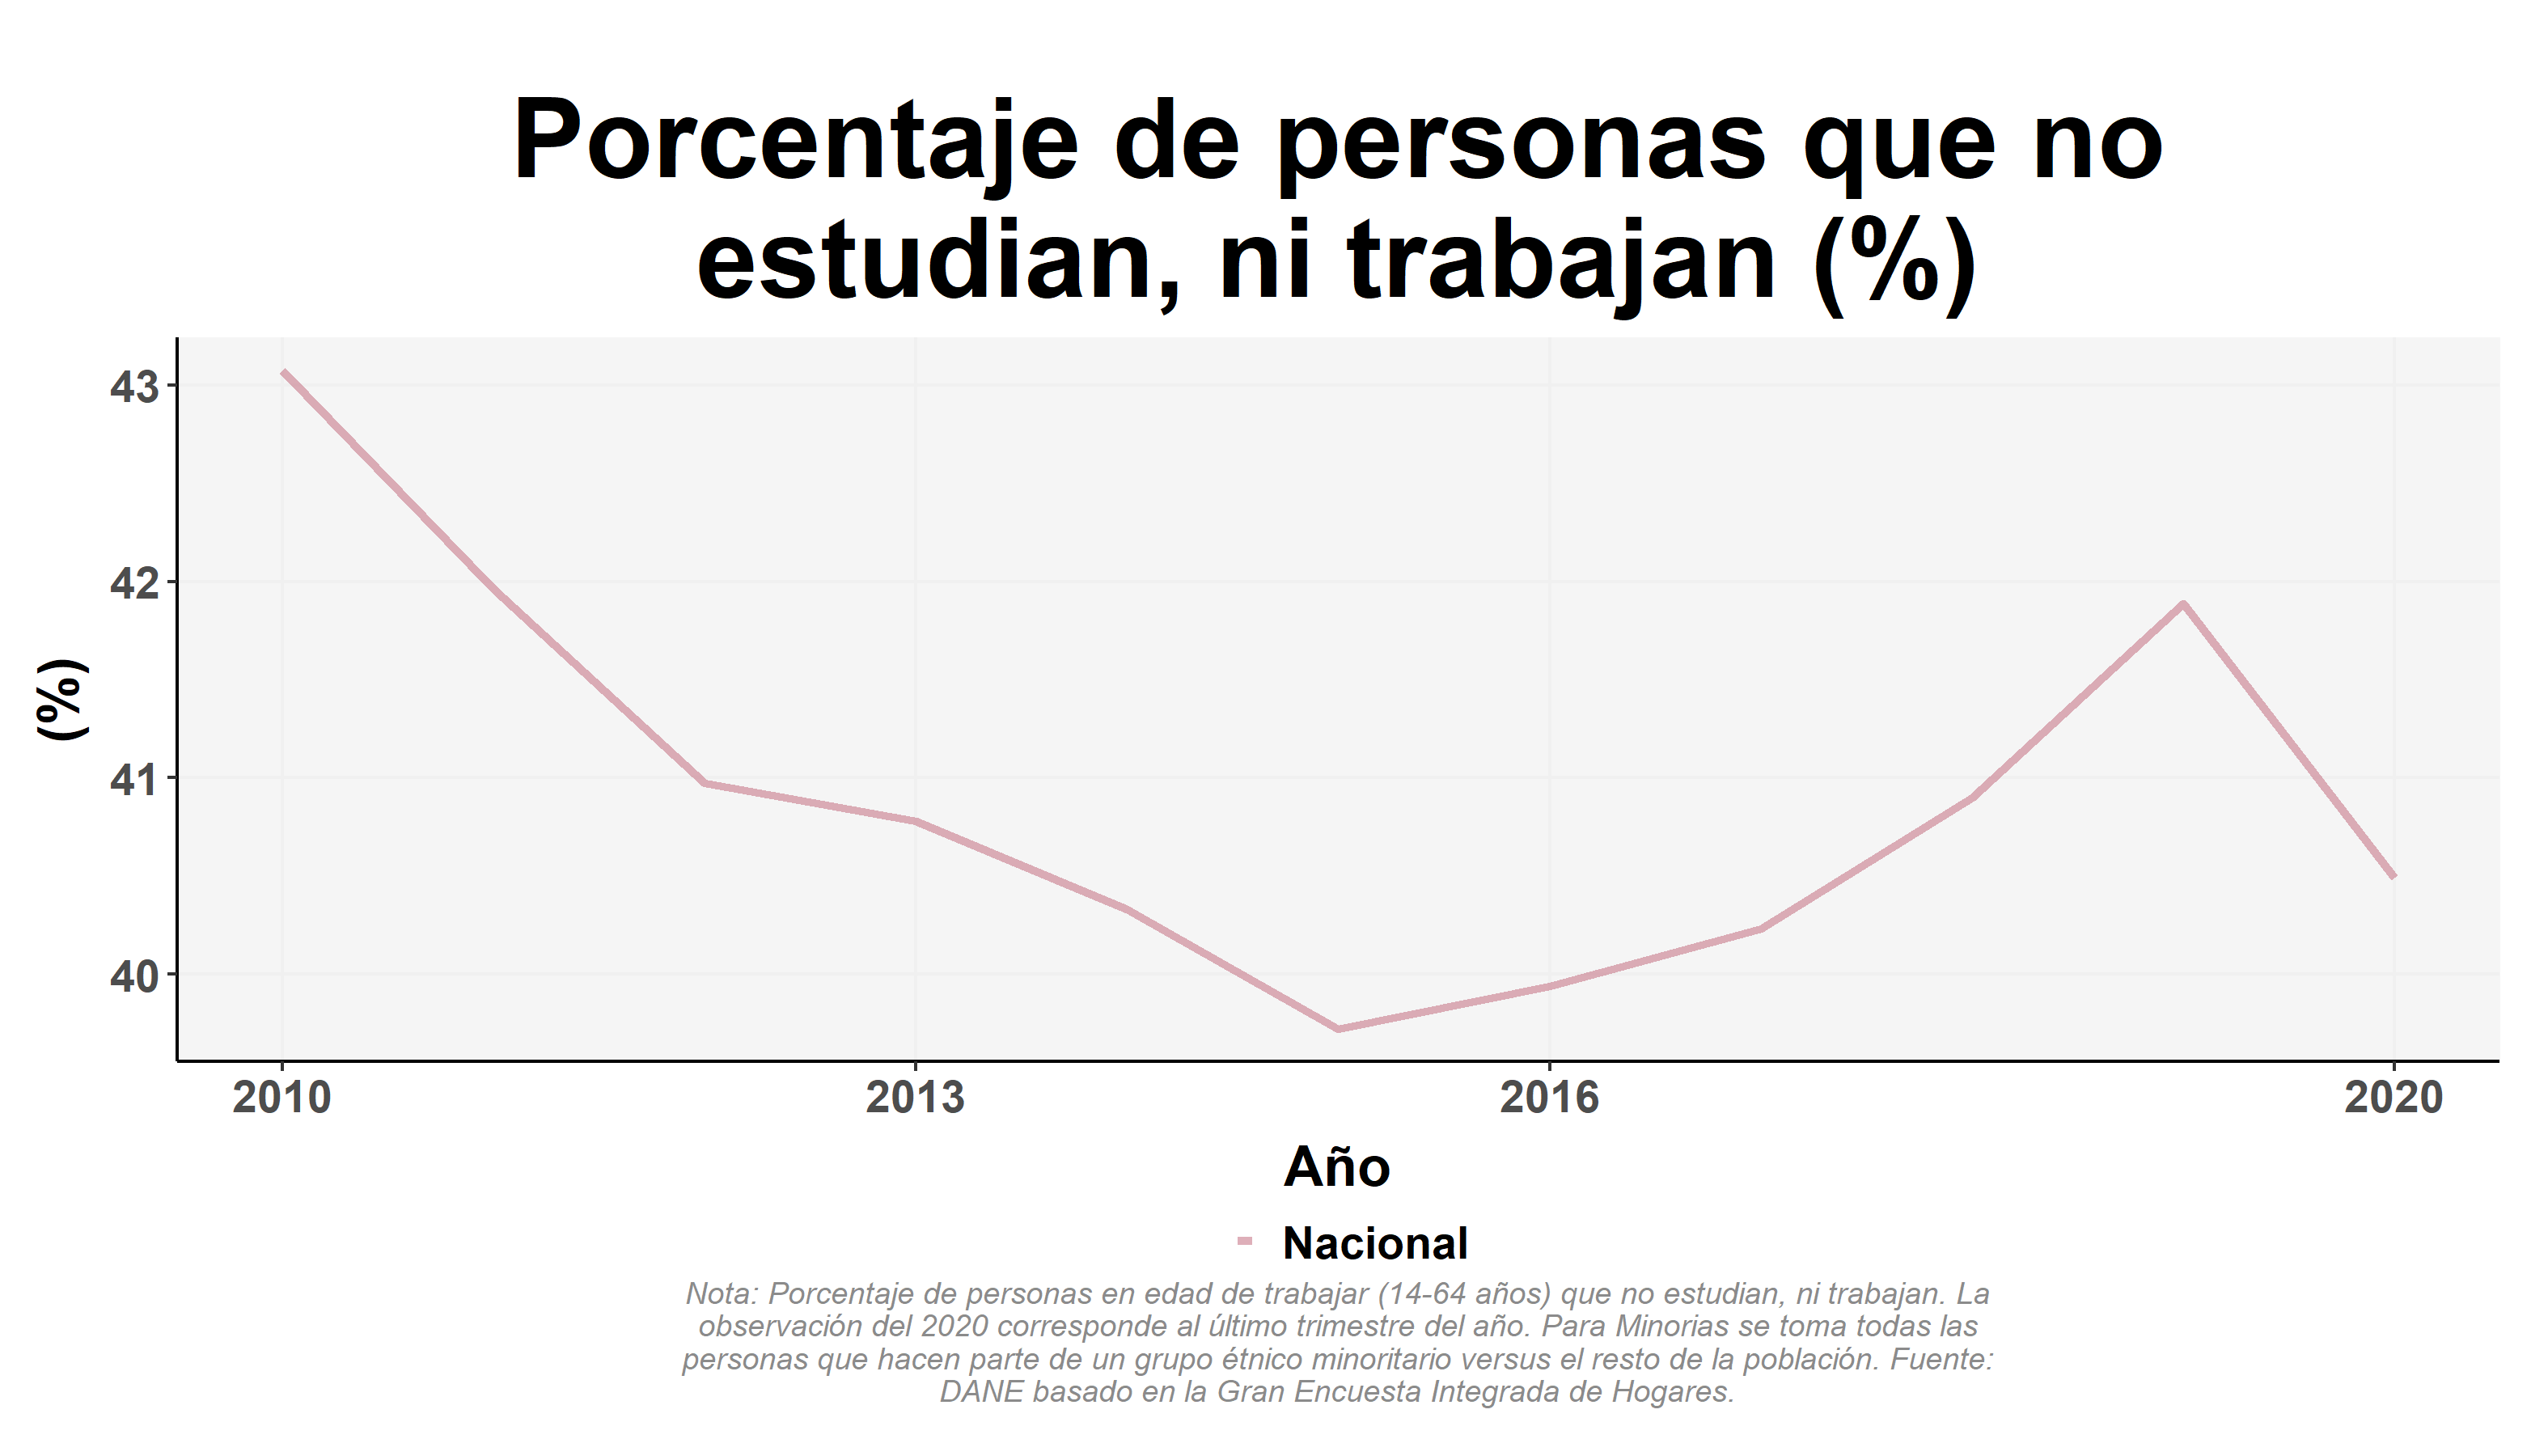
\includegraphics[width=\textwidth,keepaspectratio]{img/var_36_trend.png}
        \end{center}
    \end{figure}
            \begin{itemize}
                \item De 2010 hasta el 2015 el porcentaje de ninis estaba disminuyendo pero a partir del 2016 tuvo un incremento hasta 2019 que llegó cerca a los niveles registrados en 2011.
                \item Para 2020 a pesar de la pandemia el porcentaje de ninis disminuyó significativamente.
                \end{itemize}

%%%% Include figures
    \begin{figure}[H]
        \caption{Personas que no estudian ni trabajan por minorías y no minorías para 2020 \label{map_result_2} }
        \begin{center}
        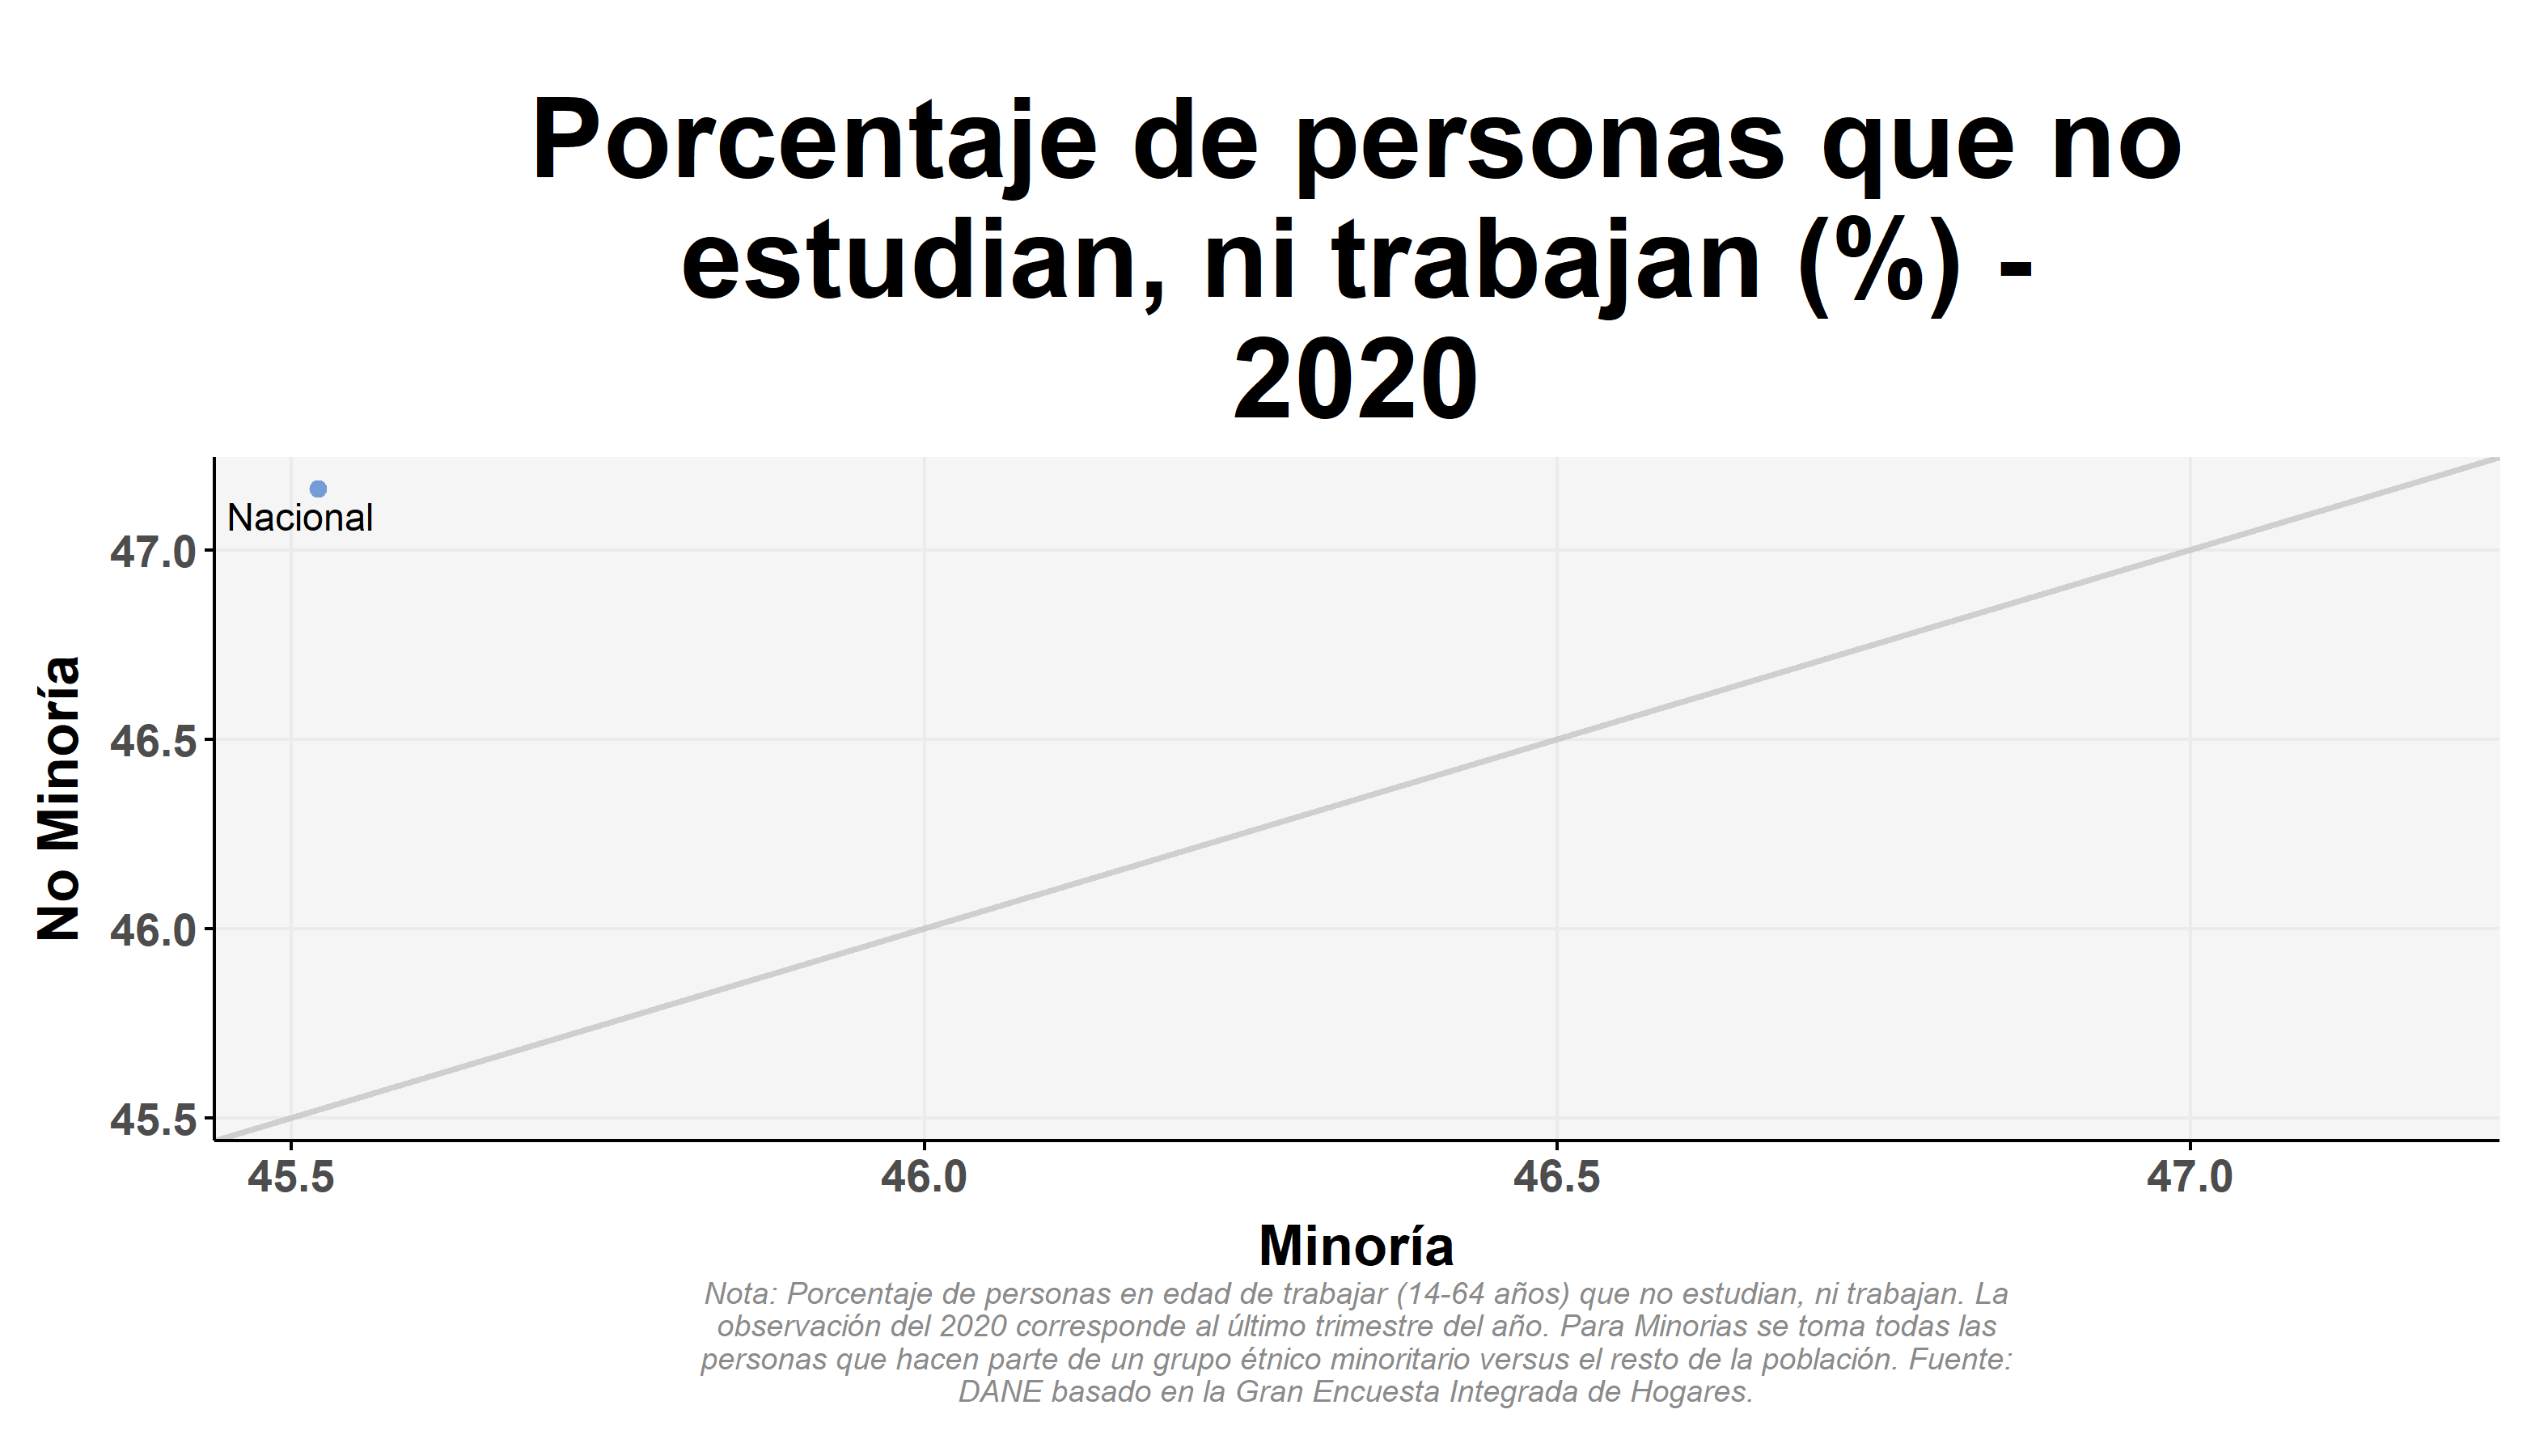
\includegraphics[width=\textwidth,keepaspectratio]{img/var_34_scatter.png}
        \end{center}
    \end{figure}
            \begin{itemize}
                \item Las minorías presentan menos porcentaje de ninis que las no minorías, aunque la diferencia entre estos es de un 2\% aproximadamente.
                \end{itemize}

        \subsubsection{Tasa de desempleo}

%%%% Include figures
    \begin{figure}[H]
        \caption{Tasa de desempleo por ciudades - 2010 VS 2020 \label{map_result_2} }
        \begin{center}
        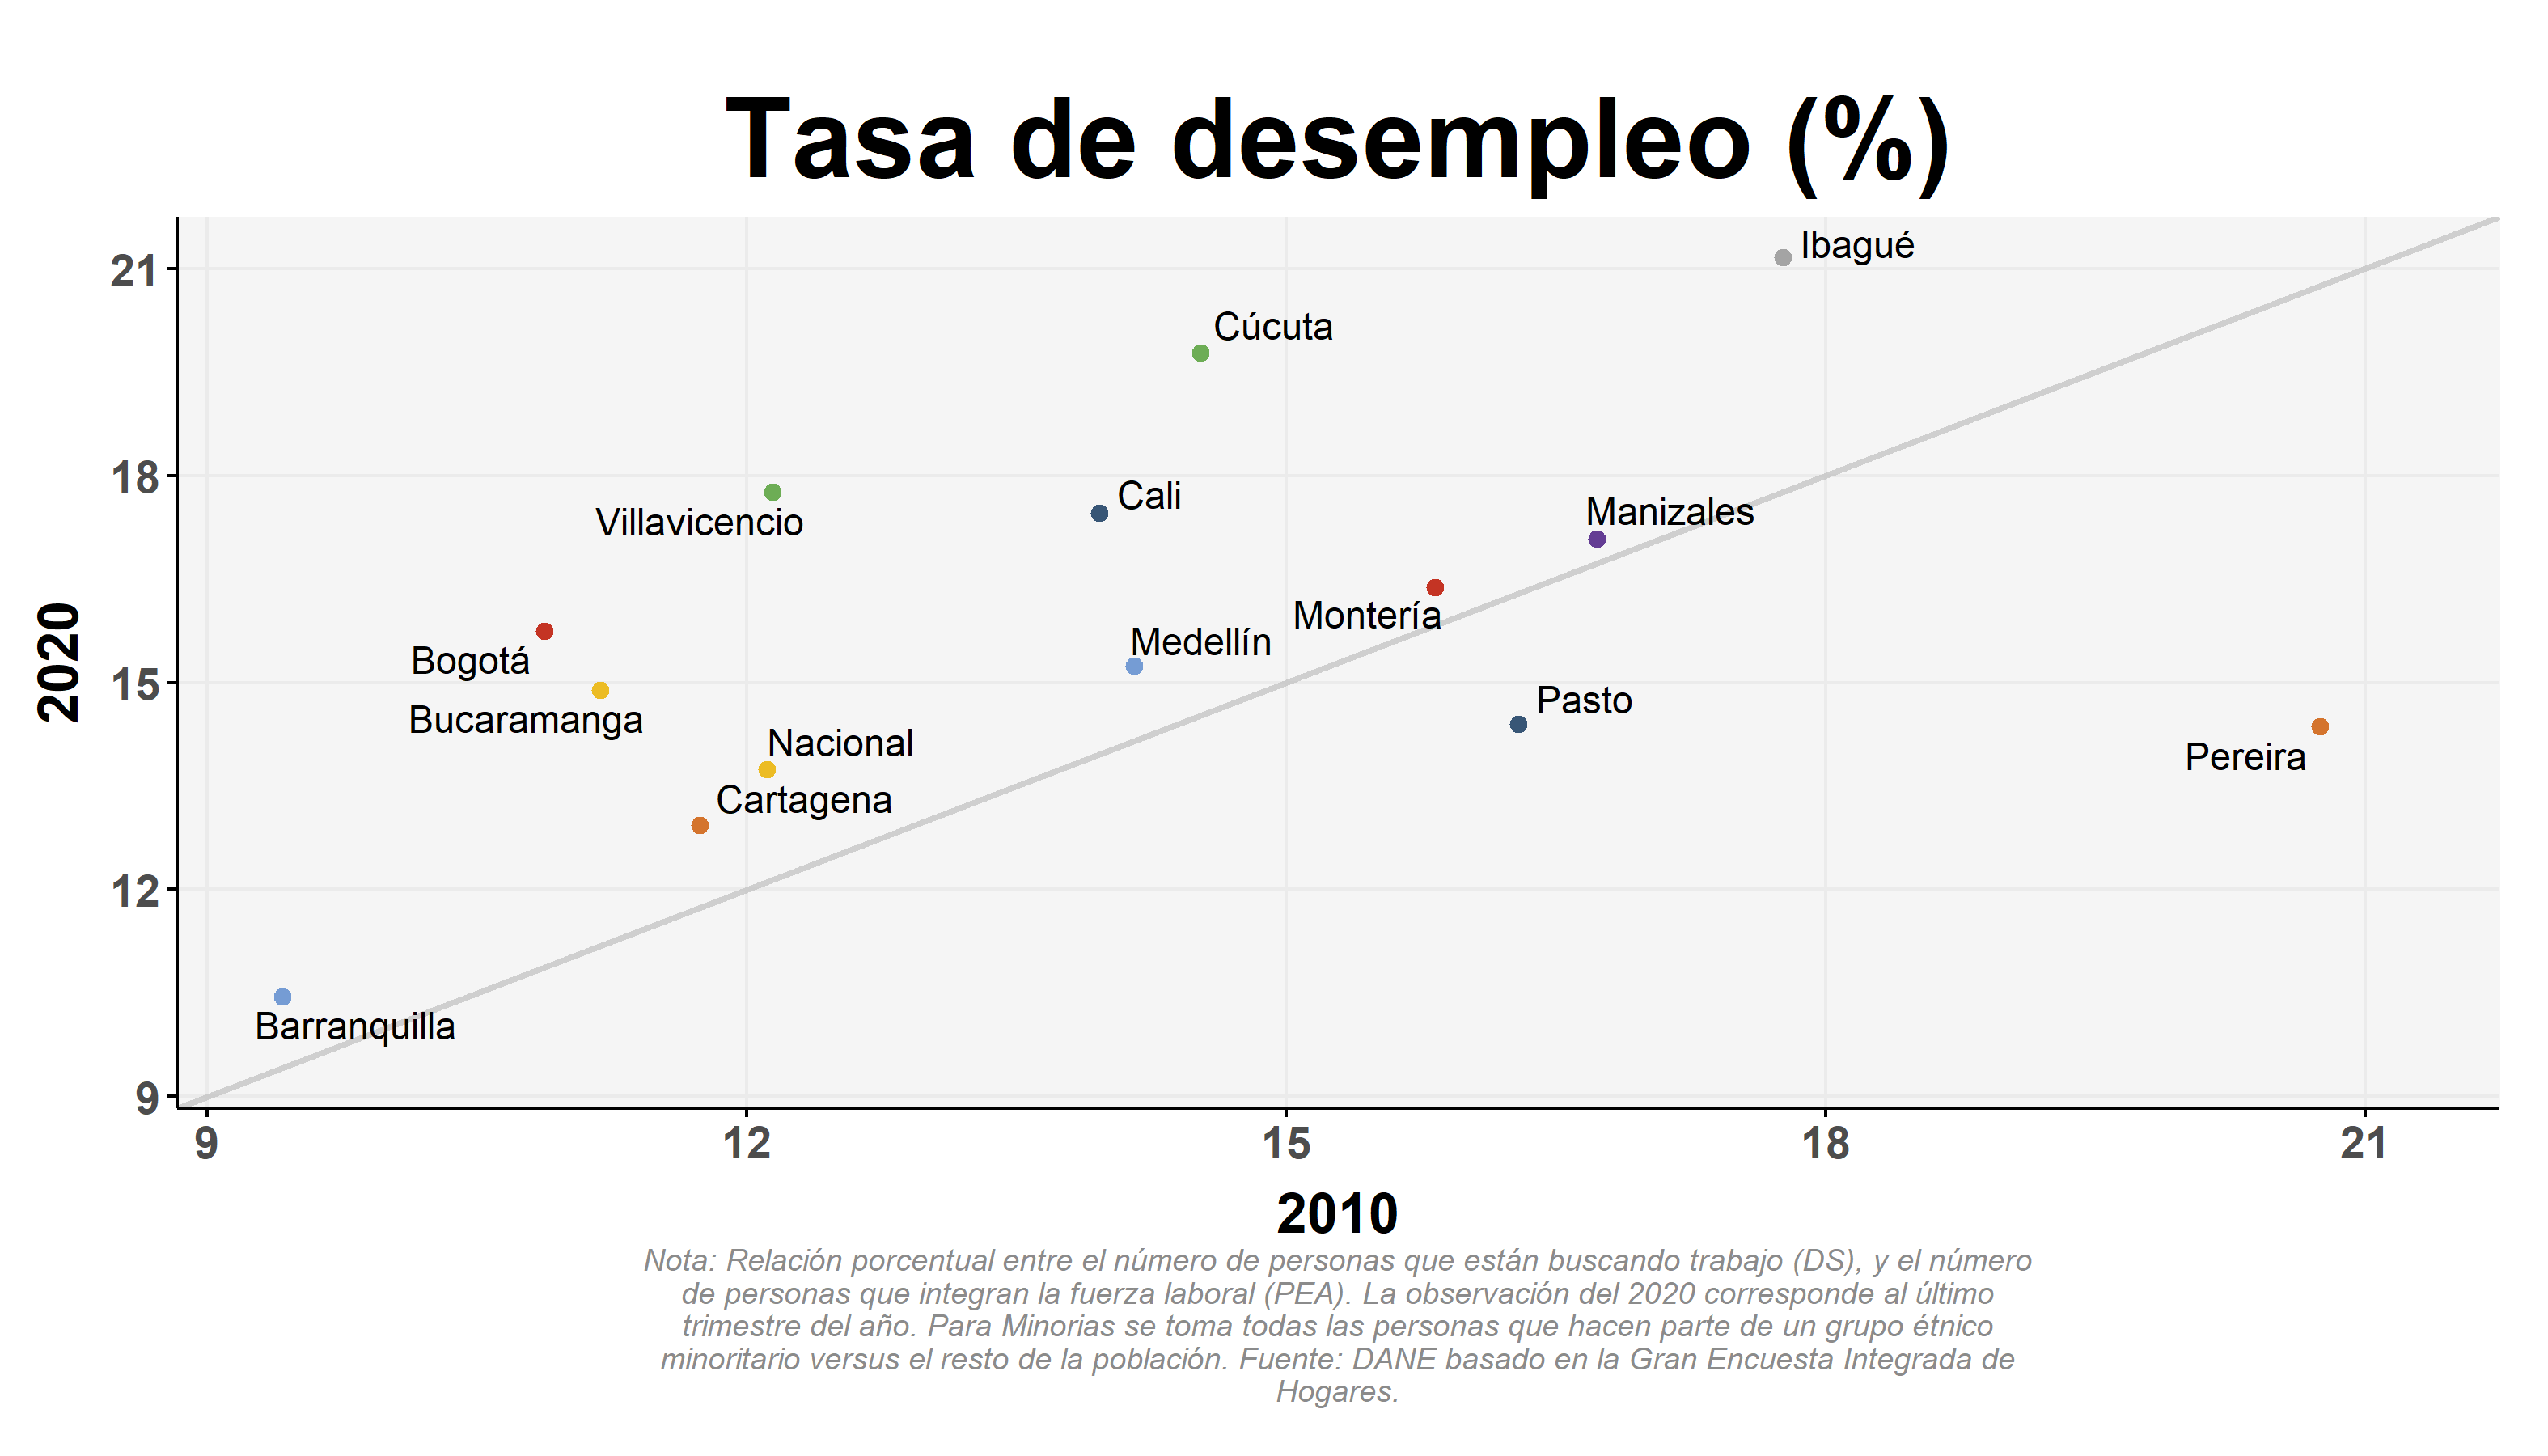
\includegraphics[width=\textwidth,keepaspectratio]{img/var_45_scatter_time.png}
        \end{center}
    \end{figure}
            \begin{itemize}
                \item Pasto y Pereira son las únicas ciudades que mostraron una mejora para 2020 con respecto a lo registrado en 2010.
                \item Se incrementó en las demás ciudades el desempleo para 2020 debido a la pandemia, especialmente en ciudades como Villavicencio, Cúcuta y Bogotá.
                \item Manizales y Montería a pesar de haber aumentado, este fue leve permitiéndoles estar cerca a los valores del 2010.
                \item No se muestra mucha variación entre las ciudades, la diferencia entre la de mayor y menor tasa es de poco más del 10\% (Ibagué - Barranquilla)
                \end{itemize}

%%%% Include figures
    \begin{figure}[H]
        \caption{Tasa de desempleo por ciudades por género para 2020 \label{map_result_2} }
        \begin{center}
        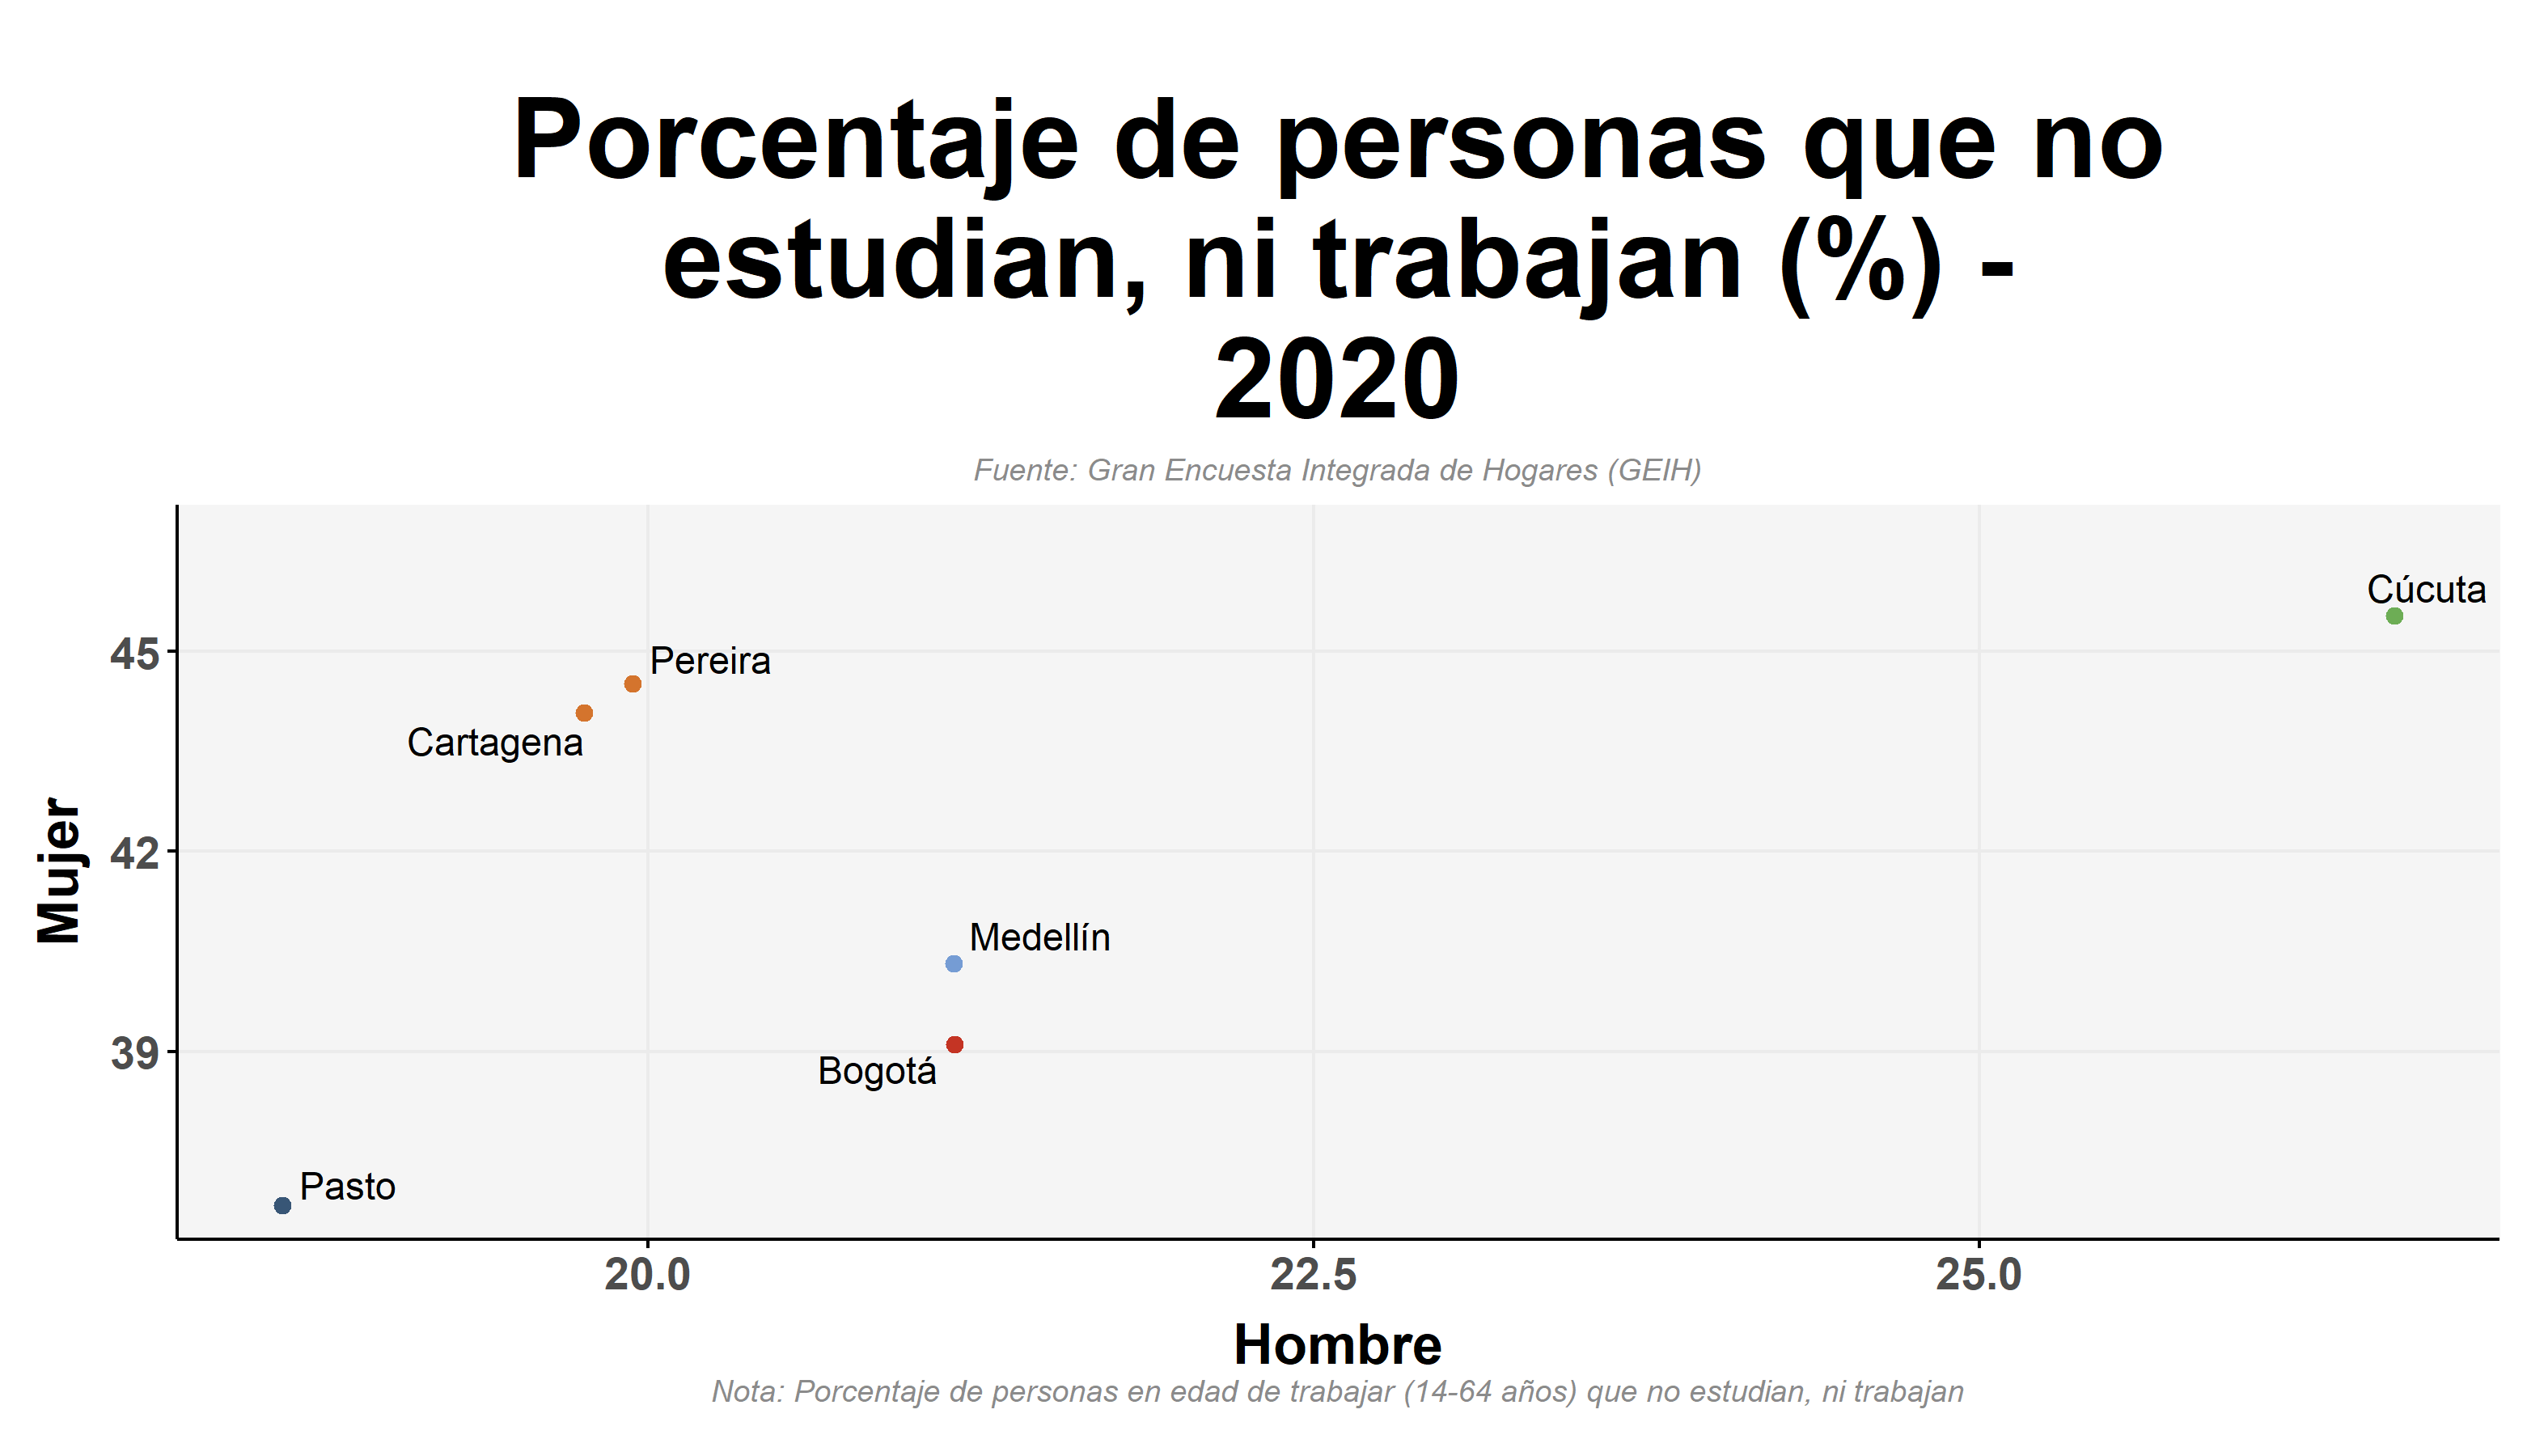
\includegraphics[width=\textwidth,keepaspectratio]{img/var_44_scatter.png}
        \end{center}
    \end{figure}
            \begin{itemize}
                \item En general en las ciudades las mujeres tienen tasas de desempleo más altas en comparación con los hombres.
                \item Bucaramanga es la ciudad en la que la brecha entre género es menor.
                \end{itemize}

%%%% Include figures
    \begin{figure}[H]
        \caption{Tasa de desempleo por ciudades por minorías y no minorías para 2020 \label{map_result_2} }
        \begin{center}
        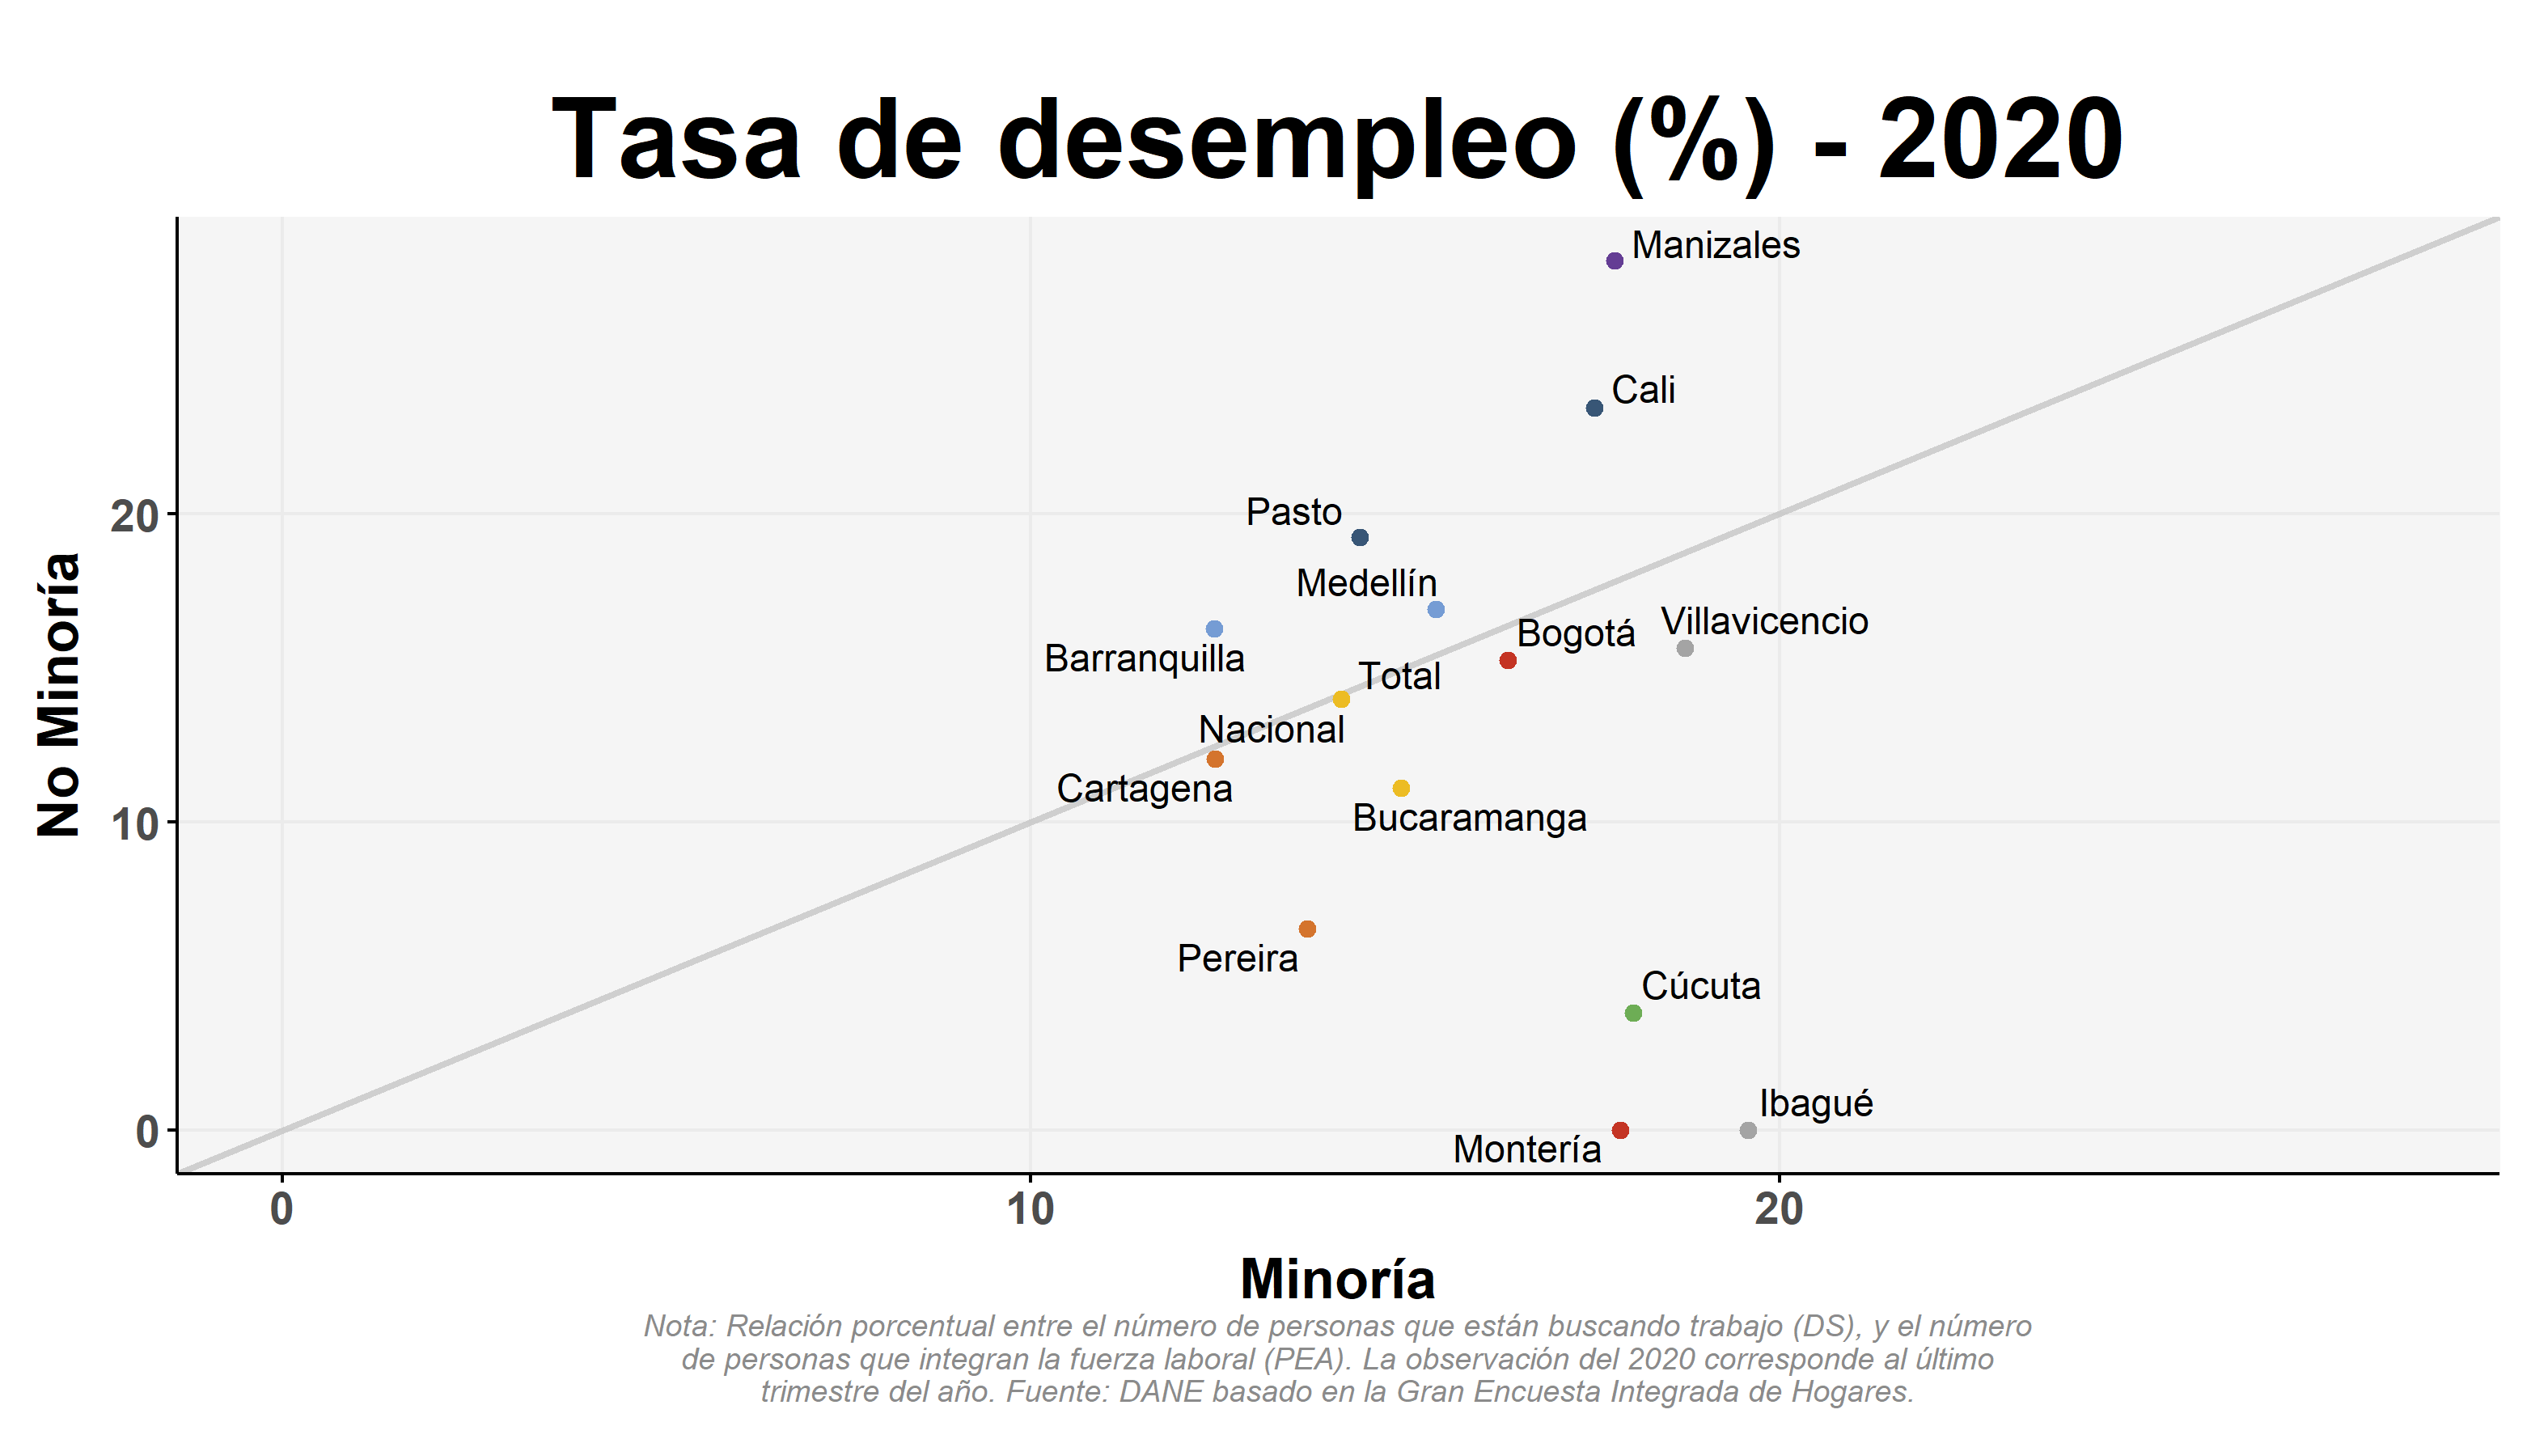
\includegraphics[width=\textwidth,keepaspectratio]{img/var_43_scatter.png}
        \end{center}
    \end{figure}
            \begin{itemize}
                \item Las oportunidades de empleo para las minorías varía según la región.
                \item Ibagué, Montería y Cúcuta son las ciudades en las que la tasa de desempleo de las minorías es más alta que el resto, mientras que en Montería y Cali son menores a las de no minorías.
                \end{itemize}

%%%% Include figures
    \begin{figure}[H]
        \caption{Tasa de desempleo por departamentos - 2010 VS 2020 \label{map_result_2} }
        \begin{center}
        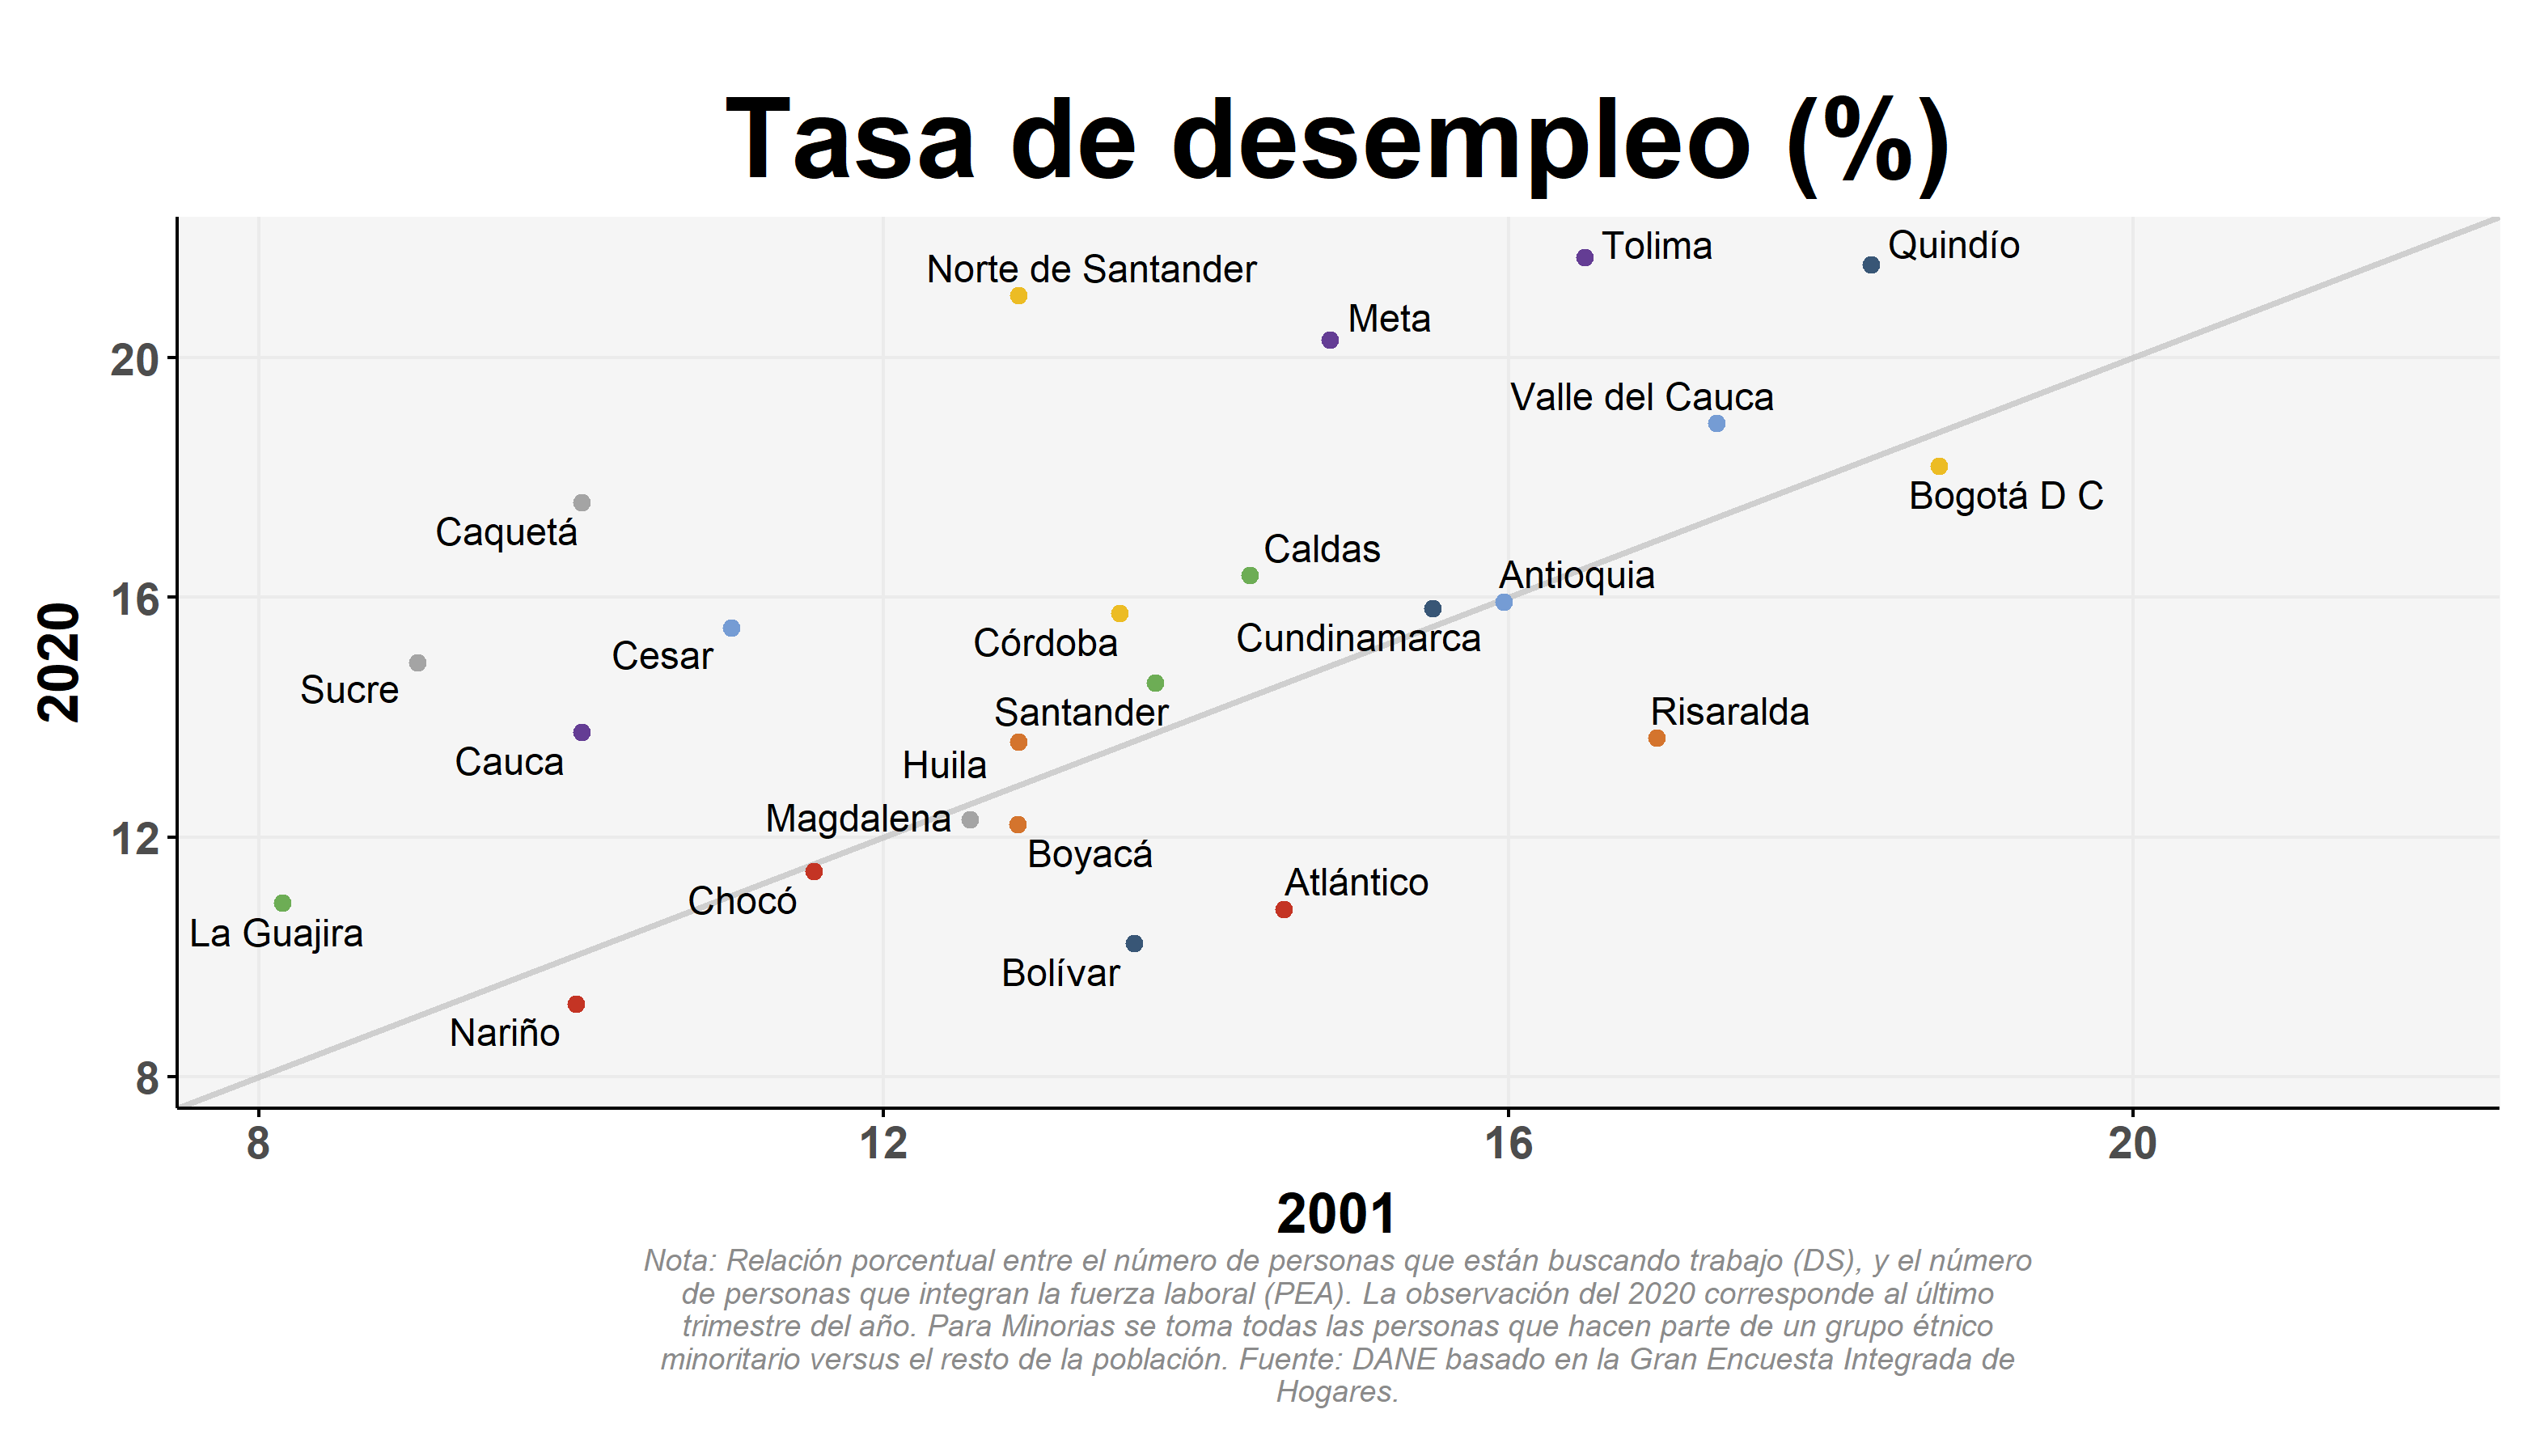
\includegraphics[width=\textwidth,keepaspectratio]{img/var_47_scatter_time.png}
        \end{center}
    \end{figure}
            \begin{itemize}
                \item En general se evidencia un aumento en la tasa de desempleo por dptos para 2020, con algunos territorios presentando mejoras.
                \item Risaralda, Atlántico y Bolívar son los dptos que presentan las mayores mejoras en el 2020 con respecto al 2010.
                \item Norte pasó de estar en el promedio a ser el tercer dpto con la tasa de desempleo más alta, mientras que Bolívar pasó a ser el segundo con la tasa más baja.
                \end{itemize}

%%%% Include figures
    \begin{figure}[H]
        \caption{Tasa de desempleo por departamentos para 2020 \label{map_result_2} }
        \begin{center}
        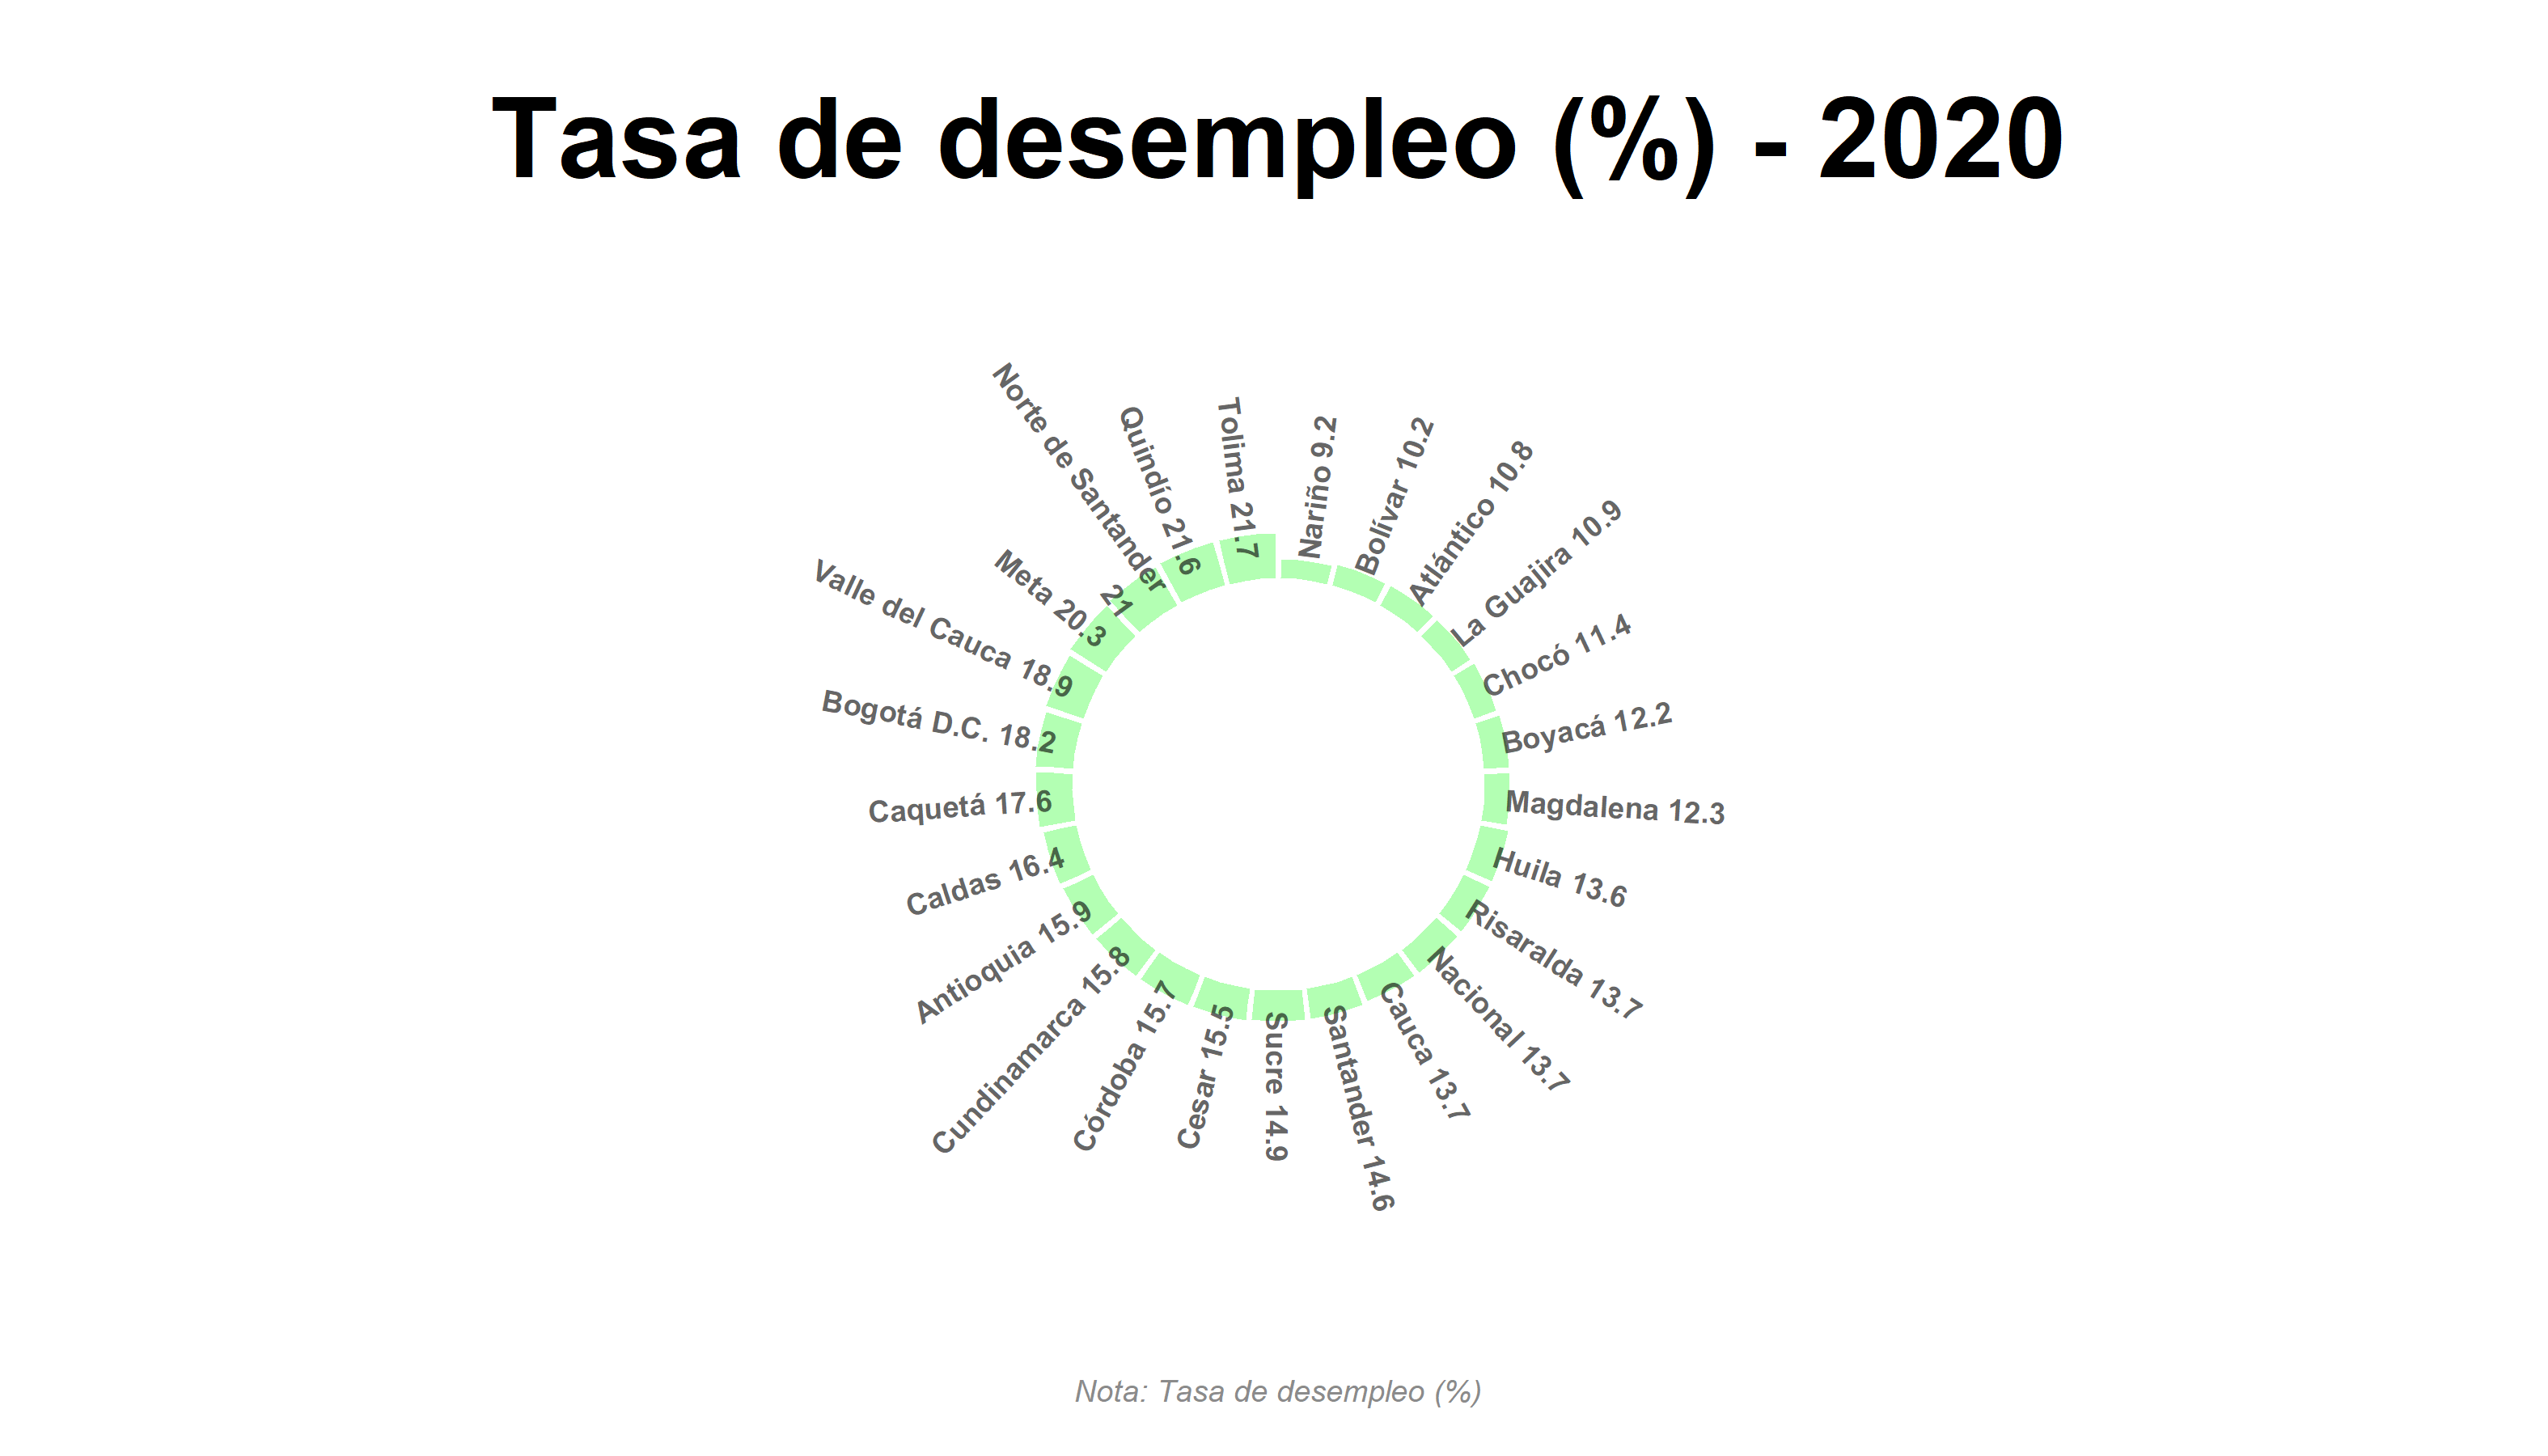
\includegraphics[width=\textwidth,keepaspectratio]{img/var_47_static.png}
        \end{center}
    \end{figure}
            \begin{itemize}
                \item Entre el dpto con mayor y menor tasa de desempleo hay una diferencia aproximadamente del 12\% (Tolima - Nariño).
                \item Las zonas con mayor tasa de desempleo se concentran en el centro del país.
                \end{itemize}

%%%% Include figures
    \begin{figure}[H]
        \caption{Tasa de desempleo a nivel nacional \label{map_result_2} }
        \begin{center}
        \includegraphics[width=\textwidth,keepaspectratio]{img/var_50_trend.png}
        \end{center}
    \end{figure}
            \begin{itemize}
                \item En la primera mitad de la década la tasa de desempleo estaba disminuyendo, pero a partir del 2016 esta inició su aumento.
                \item Aunque desde 2016 la tasa de desempleo estaba en aumento, en 2020 esta se intensificó dada la emergencia sanitaria, sobrepasando los niveles registrados en 2010.
                \end{itemize}

%%%% Include figures
    \begin{figure}[H]
        \caption{Tasa de desempleo por género \label{map_result_2} }
        \begin{center}
        \includegraphics[width=\textwidth,keepaspectratio]{img/var_49_trend.png}
        \end{center}
    \end{figure}
            \begin{itemize}
                \item La brecha de género se ha mantenido en los últimos diez años, incentivándose con la pandemia de 2020.
                \item Aunque ambas tasas aumentaron en 2020, se ve que este fue mayor en la mujer que en el hombre, pero ambos superaron los registrados en los últimos 10 años.
                \item Para 2020 el incremento en la tasa de desempleo del hombre hizo que se acercara a los niveles registrados para la mujer en el 2014, su punto más bajo.
                \end{itemize}

    \subsection{Empleo formal}

%%%% Include figures
    \begin{figure}[H]
        \caption{Tasa de formalidad por ciudades por minorías y no minorías para 2020 \label{map_result_2} }
        \begin{center}
        \includegraphics[width=\textwidth,keepaspectratio]{img/var_57_scatter.png}
        \end{center}
    \end{figure}
            \begin{itemize}
                \item En general en las principales ciudades la tasa de formalidad es mayor para las minorías.
                \item Bucaramanga, Ibagué y Cúcuta son las únicas en las que la tasa es mayor para las no minorías.
                \item Cali, Pasto y Cartagena son las ciudades en donde las tasas de ambas partes es similar.
                \end{itemize}

%%%% Include figures
    \begin{figure}[H]
        \caption{Tasa de formalidad por ciudades a nivel nacional \label{map_result_2} }
        \begin{center}
        \includegraphics[width=\textwidth,keepaspectratio]{img/var_60_trend.png}
        \end{center}
    \end{figure}
            \begin{itemize}
                \item La tasa de formalidad ha estado aumentando de manera constante con un pico para 2019.
                \item Para 2020 hay una disminución, retrocediendo aproximadamente 5 años.
                \end{itemize}

%%%% Include figures
    \begin{figure}[H]
        \caption{Tasa de formalidad por género \label{map_result_2} }
        \begin{center}
        \includegraphics[width=\textwidth,keepaspectratio]{img/var_59_trend.png}
        \end{center}
    \end{figure}
            \begin{itemize}
                \item La brecha entre ambos géneros ha ido disminuyendo al final de la década.
                \item La tasa de formalidad del hombre ha variado más en los últimos años, especialmente en el 2020, mientras que la de la mujer es menos susceptible.
                \end{itemize}

    \subsection{Empleo informal}

%%%% Include figures
    \begin{figure}[H]
        \caption{Tasa de informalidad por ciudades por minorías y no minorías para 2020 \label{map_result_2} }
        \begin{center}
        \includegraphics[width=\textwidth,keepaspectratio]{img/var_67_scatter.png}
        \end{center}
    \end{figure}
            \begin{itemize}
                \item En Bucaramanga, Ibagué y Manizales son de las ciudades donde las minorías presentan una tasa de informalidad mayor a la de las no minorías.
                \item Montería, Barranquilla, Pasto y Bogotá son las ciudades donde las minorías tienen una menor tasa de informalidad.
                \item Medellín tiene tasas de informalidad similares tanto para las no minorías y las minorías.
                \end{itemize}

%%%% Include figures
    \begin{figure}[H]
        \caption{Tasa de informalidad a nivel nacional \label{map_result_2} }
        \begin{center}
        \includegraphics[width=\textwidth,keepaspectratio]{img/var_70_trend.png}
        \end{center}
    \end{figure}
            \begin{itemize}
                \item Aunque al inicio de la década estaba disminuyendo a partir del 2015 estuvo variando significativamente.
                \item En 2020 se presenta un aumento pasando de estar en su punto más bajo en 2019 al más alto registrado en la década.
                \end{itemize}

%%%% Include figures
    \begin{figure}[H]
        \caption{Tasa de informalidad a nivel nacional \label{map_result_2} }
        \begin{center}
        \includegraphics[width=\textwidth,keepaspectratio]{img/var_69_trend.png}
        \end{center}
    \end{figure}
            \begin{itemize}
                \item Las mujeres tienden a tener tasas de informalidad más bajos que los hombres.
                \item La tasa de informalidad en los hombres ha ido aumentando, mientras que en la mujer disminuyó significativamente entre 2011 y 2015.
                \item En los últimos años la tasa de informalidad en la mujer estaba a niveles similares hasta 2020 dónde aumentó significativamente a niveles similares en el 2013, por el lado de la de los hombres en los últimos años estuvo variando y para 2020 estuvo por encima de la registrada en 2010, este suceso también pasó entre 2016 y 2018.
                \end{itemize}

    \subsection{Ingreso laboral}

%%%% Include figures
    \begin{figure}[H]
        \caption{Percentil 25 del ingreso laboral de los adultos a nivel nacional \label{map_result_2} }
        \begin{center}
        \includegraphics[width=\textwidth,keepaspectratio]{img/var_10_trend.png}
        \end{center}
    \end{figure}
            \begin{itemize}
                \item El ingreso laboral de los adultos en el percentil 25 ha estado aumentando hasta 2017 donde inicia a disminuir.
                \item Entre 2010 y 2019 el ingreso laboral para adultos ha aumentado 100 mil pesos aproximadamente con un total por debajo de los 800 mil en 2019.
                \end{itemize}

%%%% Include figures
    \begin{figure}[H]
        \caption{Percentil 25 del ingreso laboral de los adultos por género \label{map_result_2} }
        \begin{center}
        \includegraphics[width=\textwidth,keepaspectratio]{img/var_9_trend.png}
        \end{center}
    \end{figure}
            \begin{itemize}
                \item El ingreso laboral para adultos en el percentil 25 muestra una brecha de género que se ha mantenido a lo largo del tiempo de aproximadamente 200 mil pesos, siendo los hombres quienes reciben más.
                \item El ingreso laboral ha presentado mayor cambio en los hombres que en las mujeres.
                \end{itemize}

%%%% Include figures
    \begin{figure}[H]
        \caption{Percentil 25 del ingreso laboral de los adultos por ciudades - 2010 VS 2019 \label{map_result_2} }
        \begin{center}
        \includegraphics[width=\textwidth,keepaspectratio]{img/var_7_scatter_time.png}
        \end{center}
    \end{figure}
            \begin{itemize}
                \item A excepción de Bucaramanga y Cúcuta las demás ciudades principales han mejorado el ingreso laboral en el percentil 25.
                \item Cúcuta y Bucaramanga mantienen los mismos niveles de ingreso laboral que hace 10 años.
                \item Mientras Cúcuta tiene aproximadamente 700 mil como ingreso laboral Bogotá tiene 1.3 millones, es decir 600 mil pesos más aproximadamente.
                \end{itemize}

%%%% Include figures
    \begin{figure}[H]
        \caption{Percentil 25 del ingreso laboral de los adultos por ciudades por género para 2019 \label{map_result_2} }
        \begin{center}
        \includegraphics[width=\textwidth,keepaspectratio]{img/var_6_static.png}
        \end{center}
    \end{figure}
            \begin{itemize}
                \item La brecha entre ambos géneros persiste, mientras que en los hombres vemos una menor heterogeneidad en los datos, en las mujeres vemos como pueden variar mucho entre las ciudades.
                \item La diferencia entre la ciudad con más ingreso y la de menos es de 100 mil aproximadamente para los hombres y de 400 mil para las mujeres.
                \end{itemize}

%%%% Include figures
    \begin{figure}[H]
        \caption{Percentil 50 del ingreso laboral de los adultos a nivel nacional \label{map_result_2} }
        \begin{center}
        \includegraphics[width=\textwidth,keepaspectratio]{img/var_20_trend.png}
        \end{center}
    \end{figure}
            \begin{itemize}
                \item El ingreso laboral en el percentil 50 ha aumentado significativamente desde el 2012, pasando de cerca de 1.2 millones a cerca de 1.4 millones.
                \item El ingreso laboral en el percentil 50 es aproximadamente el doble del registrado en el percentil 25.
                \end{itemize}

%%%% Include figures
    \begin{figure}[H]
        \caption{Percentil 50 del ingreso laboral de los adultos por género \label{map_result_2} }
        \begin{center}
        \includegraphics[width=\textwidth,keepaspectratio]{img/var_19_trend.png}
        \end{center}
    \end{figure}
            \begin{itemize}
                \item El ingreso laboral en el percentil 50 por género muestra como en esta década se disminuyó la brecha, pasando de 100 mil aproximadamente en 2010 a menos de 50 mil en 2019.
                \item Aunque en ambos géneros el ingreso aumentó, vemos que en el de la mujer lo hizo de manera constante, mientras que en el del hombre los aumentos eran menores y en los últimos años tuvo un retroceso.
                \end{itemize}

%%%% Include figures
    \begin{figure}[H]
        \caption{Percentil 75 del ingreso laboral de los adultos a nivel nacional \label{map_result_2} }
        \begin{center}
        \includegraphics[width=\textwidth,keepaspectratio]{img/var_30_trend.png}
        \end{center}
    \end{figure}
            \begin{itemize}
                \item Aunque el ingreso estuvo aumentando hasta 2016, después de eso tuvo una fuerte caída que llevó a que en 2018 tuviera valores cercanos a los del 2013, y aunque se recuperó un poco en 2019, estos aún son similares a los de 5 años atrás.'
                \end{itemize}

%%%% Include figures
    \begin{figure}[H]
        \caption{Percentil 75 del ingreso laboral de los adultos por género \label{map_result_2} }
        \begin{center}
        \includegraphics[width=\textwidth,keepaspectratio]{img/var_29_trend.png}
        \end{center}
    \end{figure}
            \begin{itemize}
                \item En el percentil 75 la brecha de género en el ingreso laboral ha disminuido gracias al aumento del ingreso de la mujer y la disminución en el del hombre.
                \item Mientras el ingreso de la mujer ha estado aumentando en la última década el del hombre solo lo hizo hasta 2016, donde inició a disminuir llegando a que en 2019 tuviera el mismo ingreso que en 2010.
                \end{itemize}

    \subsection{Participación laboral}

%%%% Include figures
    \begin{figure}[H]
        \caption{Tasa global de participación de los adultos a nivel nacional \label{map_result_2} }
        \begin{center}
        \includegraphics[width=\textwidth,keepaspectratio]{img/var_83_trend.png}
        \end{center}
    \end{figure}
            \begin{itemize}
                \item La tasa global de participación de los adultos aumentó hasta el 2012, después estuvo estable hasta 2017 donde inició a disminuir.
                \item En 2020 la tasa global de participación cayó significativamente teniendo los niveles más bajos de la década.
                \end{itemize}

%%%% Include figures
    \begin{figure}[H]
        \caption{Tasa global de participación de los adultos por género \label{map_result_2} }
        \begin{center}
        \includegraphics[width=\textwidth,keepaspectratio]{img/var_82_trend.png}
        \end{center}
    \end{figure}
            \begin{itemize}
                \item La tasa global de participación se mantuvo constante, para la tasa del hombre solo se ve un descenso en 2020 mientras que en la mujer el descenso viene desde 2017 que se intensificó en 2020 a causa de la pandemia.
                \item La brecha entre los géneros es de aproximadamente un 20\% siendo siempre la del hombre mayor a la mujer.
                \end{itemize}

%%%% Include figures
    \begin{figure}[H]
        \caption{Tasa global de participación a nivel nacional \label{map_result_2} }
        \begin{center}
        \includegraphics[width=\textwidth,keepaspectratio]{img/var_80_trend.png}
        \end{center}
    \end{figure}
            \begin{itemize}
                \item La tasa global de participación total a nivel nacional se mantuvo en niveles similares a lo largo de la década y para 2020 se disparó significativamente.
                \end{itemize}

%%%% Include figures
    \begin{figure}[H]
        \caption{Tasa global de participación por género/ \label{map_result_2} }
        \begin{center}
        \includegraphics[width=\textwidth,keepaspectratio]{img/var_79_trend.png}
        \end{center}
    \end{figure}
            \begin{itemize}
                \item Al igual que la tasa global de participación de los adultos la tasa total se comporta de manera similar, manteniendo niveles constante hasta el 2020 donde tiene una caída que supera los niveles en 2010.
                \end{itemize}

%%%% Include figures
    \begin{figure}[H]
        \caption{Tasa global de participación por ciudades por minorías y no minorías \label{map_result_2} }
        \begin{center}
        \includegraphics[width=\textwidth,keepaspectratio]{img/var_80_trend.png}
        \end{center}
    \end{figure}
            \begin{itemize}
                \item Para todas las ciudades principales la tasa global de participación es mayor para las no minorías que las minorías.
                \item Manizales, Pereira y Cali son las únicas ciudades donde la tasa de participación para las minorías y no minorías son similares.
                \item A nivel nacional la tasa de participación es mayor para las minorías que las no minorías.
                \end{itemize}

    \subsection{Escolaridad}

%%%% Include figures
    \begin{figure}[H]
        \caption{Diferencia en los años de educación promedio entre indígenas y no indígenas para 2020 \label{map_result_2} }
        \begin{center}
        \includegraphics[width=\textwidth,keepaspectratio]{img/var_123_static.png}
        \end{center}
    \end{figure}
            \begin{itemize}
                \item Tres cuartos de los dptos las personas no indígenas en promedio tienen más años que los indígenas.
                \item Amazonas, Córdoba y Nariño en promedio tienen un año o más de educación los indígenas con respecto a los no indígenas.
                \item Guaviare es el dpto donde las personas no indígenas tienen caso 2.6 años más de educación con respecto a los indígenas.
                \end{itemize}

%%%% Include figures
    \begin{figure}[H]
        \caption{Diferencia en los años de educación promedio entre indígenas y no indígenas por zonas \label{map_result_2} }
        \begin{center}
        \includegraphics[width=\textwidth,keepaspectratio]{img/var_124_trend.png}
        \end{center}
    \end{figure}
            \begin{itemize}
                \item Las zonas rurales han disminuido la diferencia de años entre indígenas y no indígenas manteniendo un aumento constante.
                \item En las cabeceras los años aumentaron para los indígenas al inicio de la década con una caída en 2016 y a partir del 2018 inició a disminuir y para 2020 llegó a niveles similares para las cabeceras y rurales.
                \end{itemize}

    \subsection{Muerte violenta}

%%%% Include figures
    \begin{figure}[H]
        \caption{Agresiones (homicidios) por departamentos - 2010 VS 2020 \label{map_result_2} }
        \begin{center}
        \includegraphics[width=\textwidth,keepaspectratio]{img/var_286_scatter_time.png}
        \end{center}
    \end{figure}
            \begin{itemize}
                \item Guainía, Chocó, Bolívar y San Andrés son los dptos en donde los homicidios aumentaron para 2020 con respecto a los registrados en 2010.
                \item Sucre, Atlántico y Cauca para 2020 tienen los mismos niveles de homicidios  que se registraron en 2010.
                \item Los demás dptos han disminuido los casos para 2020, en especial Guaviare, Arauca y Antioquia bajaron considerablemente, pasando de liderar la lista a estar en el promedio, en especial Guaviare. 
                \end{itemize}

%%%% Include figures
    \begin{figure}[H]
        \caption{Agresiones (homicidios) por departamentos (mapa) - 2010 VS 2020 \label{map_result_2} }
        \begin{center}
        \includegraphics[width=\textwidth,keepaspectratio]{img/var_286_map.png}
        \end{center}
    \end{figure}
            \begin{itemize}
                \item Los dptos con mayor concentración de homicidios se encuentran en la zonas sur-occidental del país.
                \item En el centro y oriente del país se encuentran los dptos con el menor nivel de homicidios para 2020.
                \end{itemize}

%%%% Include figures
    \begin{figure}[H]
        \caption{Agresiones (homicidios) por departamentos para 2020 \label{map_result_2} }
        \begin{center}
        \includegraphics[width=\textwidth,keepaspectratio]{img/var_286_static.png}
        \end{center}
    \end{figure}
            \begin{itemize}
                \item Para 2020 se denota la heterogeneidad entre dptos, mientras Vaupés es el del menor número de homicidios con 4.5 muertes por cada 100 mil habitantes, San Andrés tiene la mayor tasa de homicidios con 59.7 muertes por cada 100 mil habitantes.
                \end{itemize}

%%%% Include figures
    \begin{figure}[H]
        \caption{Agresiones (homicidios) a nivel nacional \label{map_result_2} }
        \begin{center}
        \includegraphics[width=\textwidth,keepaspectratio]{img/var_289_trend.png}
        \end{center}
    \end{figure}
            \begin{itemize}
                \item Los homicidios disminuyeron constantemente hasta 2016, donde empezó a mantener valores constantes.
                \item En 2020 hubo una caída significante, probablemente a causa de la pandemia.
                \end{itemize}

%%%% Include figures
    \begin{figure}[H]
        \caption{Agresiones (homicidios) por rango de edad \label{map_result_2} }
        \begin{center}
        \includegraphics[width=\textwidth,keepaspectratio]{img/var_287_trend.png}
        \end{center}
    \end{figure}
            \begin{itemize}
                \item Las tasas de homicidios han ido disminuyendo en la última década.
                \item La mayor concentración de homicidios se encuentra en personas entre 15 a 44 años con 20 muertes por cada 100 mil habitantes, seguido por las personas de 45 a 64 años.
                \item El rango más alto y el más bajo de edades son los de la menor tasas de homicidios.
                \end{itemize}

%%%% Include figures
    \begin{figure}[H]
        \caption{Agresiones (homicidios) por género \label{map_result_2} }
        \begin{center}
        \includegraphics[width=\textwidth,keepaspectratio]{img/var_286_map.png}
        \end{center}
    \end{figure}
            \begin{itemize}
                \item Los hombres son más propensos a homicidios que las mujeres, aunque ha venido disminuyendo con el tiempo.
                \item Para 2020 la tasa del hombre era 20 muertes más por cada 100 mil habitantes que la tasa de la mujer.
                \end{itemize}

    \subsection{Salud mental}

%%%% Include figures
    \begin{figure}[H]
        \caption{Lesiones autoinfligidas intencionalmente (suicidios) por departamentos - 2010 VS 2020 \label{map_result_2} }
        \begin{center}
        \includegraphics[width=\textwidth,keepaspectratio]{img/var_294_scatter_time.png}
        \end{center}
    \end{figure}
            \begin{itemize}
                \item En general gran parte de los dptos han mantenido los mismos niveles para 2020 comparado con los de 2010.
                \item Amazonas y Vaupés aumentaron significativamente las tasas de suicidios estando por encima de 20 muertes por cada 100 mil habitantes mientras que los demás no pasan de las 10 muertes.
                \item Amazonas pasó de ser uno de los dptos con menor tasa de suicidios a tener la segunda tasa más alta.
                \end{itemize}

%%%% Include figures
    \begin{figure}[H]
        \caption{Lesiones autoinfligidas intencionalmente (suicidios) por departamentos (mapa) - 2010 VS 2020 \label{map_result_2} }
        \begin{center}
        \includegraphics[width=\textwidth,keepaspectratio]{img/var_294_map.png}
        \end{center}
    \end{figure}
            \begin{itemize}
                \item En la zona sur y centro del país aumentaron los suicidios entre los dos años.
                \item El Amazonas es el dpto que presenta el mayor cambio en cuanto al aumento de suicidios mientras que Cundinamarca y Boyacá disminuyeron significativamente.
                \end{itemize}

%%%% Include figures
    \begin{figure}[H]
        \caption{Lesiones autoinfligidas intencionalmente (suicidios) por departamentos por género \label{map_result_2} }
        \begin{center}
        \includegraphics[width=\textwidth,keepaspectratio]{img/var_293_scatter_time.png}
        \end{center}
    \end{figure}
            \begin{itemize}
                \item Vaupés es el único dpto que la tasa de suicidios es mayor para las mujeres que para los hombres.
                \item Amazonas es el de la mayor tasa de suicidios en hombres, teniendo una diferencia de 10 muertes entre él y el segundo dpto para la tasa de hombres.
                \end{itemize}

%%%% Include figures
    \begin{figure}[H]
        \caption{Lesiones autoinfligidas intencionalmente (suicidios) a nivel nacional \label{map_result_2} }
        \begin{center}
        \includegraphics[width=\textwidth,keepaspectratio]{img/var_297_trend.png}
        \end{center}
    \end{figure}
            \begin{itemize}
                \item Aunque al inicio de la década se mantuvo a niveles constantes la tasa de suicidio, desde 2014 han ido aumentando de manera constante.
                \item En 2020 la tasa de suicidios disminuyó significativamente a causa de la pandemia.
                \end{itemize}

%%%% Include figures
    \begin{figure}[H]
        \caption{Lesiones autoinfligidas intencionalmente (suicidios) por género \label{map_result_2} }
        \begin{center}
        \includegraphics[width=\textwidth,keepaspectratio]{img/var_296_trend.png}
        \end{center}
    \end{figure}
            \begin{itemize}
                \item Los suicidios estaban aumentando hasta 2018 para los hombres y 2019 para la mujer, después de eso inició a descender.
                \item Es más común el suicidio en los hombres siendo poco más de 4 muertes por cada 100 mil habitantes mientras que en la mujer es de 1 muerte.
                \item 
                \end{itemize}

%%%% Include figures
    \begin{figure}[H]
        \caption{Lesiones autoinfligidas intencionalmente (suicidios) por grupos de edad \label{map_result_2} }
        \begin{center}
        \includegraphics[width=\textwidth,keepaspectratio]{img/var_295_trend.png}
        \end{center}
    \end{figure}
            \begin{itemize}
                \item Los suicidios son más común en personas entre 15 y 44 años, seguido por los de 45 a 64 años.
                \item En los rangos de edad más bajo y más alto las tasa de suicidio ha ido aumentando en una pequeña medida.
                \end{itemize}

\section{Vejez}
    \subsection{Enfermedades no transmisibles y obesidad}
        \subsubsection{REVISAR SECCIÓN Defunciones prematuras}

%%%% Include figures
    \begin{figure}[H]
        \caption{Defunciones prematuras a nivel nacional \label{map_result_2} }
        \begin{center}
        \includegraphics[width=\textwidth,keepaspectratio]{img/var_281_trend.png}
        \end{center}
    \end{figure}
            \begin{itemize}
                \item El numero de menores de 1 año fallecidos ha disminuido a lo largo de la década, en especial en 2020 donde tuvo una caída significativa.
                \end{itemize}

%%%% Include figures
    \begin{figure}[H]
        \caption{Defunciones prematuras por departamento - Cambio porcentual entre 2010 y 2020 \label{map_result_2} }
        \begin{center}
        \includegraphics[width=\textwidth,keepaspectratio]{img/var_280_map_change.png}
        \end{center}
    \end{figure}
            \begin{itemize}
                \item En la parte central y sur del país se encuentran los dptos donde más disminuyó las muertes prematuras.
                \item En la zona oriental se encuentran los dptos con el mayor aumento en las defunciones prematuras.
                \end{itemize}
